% Options for packages loaded elsewhere
\PassOptionsToPackage{unicode}{hyperref}
\PassOptionsToPackage{hyphens}{url}
\PassOptionsToPackage{dvipsnames,svgnames,x11names}{xcolor}
%
\documentclass[
  ignorenonframetext,
]{beamer}
\usepackage{pgfpages}
\setbeamertemplate{caption}[numbered]
\setbeamertemplate{caption label separator}{: }
\setbeamercolor{caption name}{fg=normal text.fg}
\beamertemplatenavigationsymbolsempty
% Prevent slide breaks in the middle of a paragraph
\widowpenalties 1 10000
\raggedbottom
\setbeamertemplate{part page}{
  \centering
  \begin{beamercolorbox}[sep=16pt,center]{part title}
    \usebeamerfont{part title}\insertpart\par
  \end{beamercolorbox}
}
\setbeamertemplate{section page}{
  \centering
  \begin{beamercolorbox}[sep=12pt,center]{part title}
    \usebeamerfont{section title}\insertsection\par
  \end{beamercolorbox}
}
\setbeamertemplate{subsection page}{
  \centering
  \begin{beamercolorbox}[sep=8pt,center]{part title}
    \usebeamerfont{subsection title}\insertsubsection\par
  \end{beamercolorbox}
}
\AtBeginPart{
  \frame{\partpage}
}
\AtBeginSection{
  \ifbibliography
  \else
    \frame{\sectionpage}
  \fi
}
\AtBeginSubsection{
  \frame{\subsectionpage}
}
\usepackage{amsmath,amssymb}
\usepackage{iftex}
\ifPDFTeX
  \usepackage[T1]{fontenc}
  \usepackage[utf8]{inputenc}
  \usepackage{textcomp} % provide euro and other symbols
\else % if luatex or xetex
  \usepackage{unicode-math} % this also loads fontspec
  \defaultfontfeatures{Scale=MatchLowercase}
  \defaultfontfeatures[\rmfamily]{Ligatures=TeX,Scale=1}
\fi
\usepackage{lmodern}
\usetheme[]{CambridgeUS}
\ifPDFTeX\else
  % xetex/luatex font selection
\fi
% Use upquote if available, for straight quotes in verbatim environments
\IfFileExists{upquote.sty}{\usepackage{upquote}}{}
\IfFileExists{microtype.sty}{% use microtype if available
  \usepackage[]{microtype}
  \UseMicrotypeSet[protrusion]{basicmath} % disable protrusion for tt fonts
}{}
\makeatletter
\@ifundefined{KOMAClassName}{% if non-KOMA class
  \IfFileExists{parskip.sty}{%
    \usepackage{parskip}
  }{% else
    \setlength{\parindent}{0pt}
    \setlength{\parskip}{6pt plus 2pt minus 1pt}}
}{% if KOMA class
  \KOMAoptions{parskip=half}}
\makeatother
\usepackage{xcolor}
\newif\ifbibliography
\usepackage{color}
\usepackage{fancyvrb}
\newcommand{\VerbBar}{|}
\newcommand{\VERB}{\Verb[commandchars=\\\{\}]}
\DefineVerbatimEnvironment{Highlighting}{Verbatim}{commandchars=\\\{\}}
% Add ',fontsize=\small' for more characters per line
\usepackage{framed}
\definecolor{shadecolor}{RGB}{248,248,248}
\newenvironment{Shaded}{\begin{snugshade}}{\end{snugshade}}
\newcommand{\AlertTok}[1]{\textcolor[rgb]{0.94,0.16,0.16}{#1}}
\newcommand{\AnnotationTok}[1]{\textcolor[rgb]{0.56,0.35,0.01}{\textbf{\textit{#1}}}}
\newcommand{\AttributeTok}[1]{\textcolor[rgb]{0.13,0.29,0.53}{#1}}
\newcommand{\BaseNTok}[1]{\textcolor[rgb]{0.00,0.00,0.81}{#1}}
\newcommand{\BuiltInTok}[1]{#1}
\newcommand{\CharTok}[1]{\textcolor[rgb]{0.31,0.60,0.02}{#1}}
\newcommand{\CommentTok}[1]{\textcolor[rgb]{0.56,0.35,0.01}{\textit{#1}}}
\newcommand{\CommentVarTok}[1]{\textcolor[rgb]{0.56,0.35,0.01}{\textbf{\textit{#1}}}}
\newcommand{\ConstantTok}[1]{\textcolor[rgb]{0.56,0.35,0.01}{#1}}
\newcommand{\ControlFlowTok}[1]{\textcolor[rgb]{0.13,0.29,0.53}{\textbf{#1}}}
\newcommand{\DataTypeTok}[1]{\textcolor[rgb]{0.13,0.29,0.53}{#1}}
\newcommand{\DecValTok}[1]{\textcolor[rgb]{0.00,0.00,0.81}{#1}}
\newcommand{\DocumentationTok}[1]{\textcolor[rgb]{0.56,0.35,0.01}{\textbf{\textit{#1}}}}
\newcommand{\ErrorTok}[1]{\textcolor[rgb]{0.64,0.00,0.00}{\textbf{#1}}}
\newcommand{\ExtensionTok}[1]{#1}
\newcommand{\FloatTok}[1]{\textcolor[rgb]{0.00,0.00,0.81}{#1}}
\newcommand{\FunctionTok}[1]{\textcolor[rgb]{0.13,0.29,0.53}{\textbf{#1}}}
\newcommand{\ImportTok}[1]{#1}
\newcommand{\InformationTok}[1]{\textcolor[rgb]{0.56,0.35,0.01}{\textbf{\textit{#1}}}}
\newcommand{\KeywordTok}[1]{\textcolor[rgb]{0.13,0.29,0.53}{\textbf{#1}}}
\newcommand{\NormalTok}[1]{#1}
\newcommand{\OperatorTok}[1]{\textcolor[rgb]{0.81,0.36,0.00}{\textbf{#1}}}
\newcommand{\OtherTok}[1]{\textcolor[rgb]{0.56,0.35,0.01}{#1}}
\newcommand{\PreprocessorTok}[1]{\textcolor[rgb]{0.56,0.35,0.01}{\textit{#1}}}
\newcommand{\RegionMarkerTok}[1]{#1}
\newcommand{\SpecialCharTok}[1]{\textcolor[rgb]{0.81,0.36,0.00}{\textbf{#1}}}
\newcommand{\SpecialStringTok}[1]{\textcolor[rgb]{0.31,0.60,0.02}{#1}}
\newcommand{\StringTok}[1]{\textcolor[rgb]{0.31,0.60,0.02}{#1}}
\newcommand{\VariableTok}[1]{\textcolor[rgb]{0.00,0.00,0.00}{#1}}
\newcommand{\VerbatimStringTok}[1]{\textcolor[rgb]{0.31,0.60,0.02}{#1}}
\newcommand{\WarningTok}[1]{\textcolor[rgb]{0.56,0.35,0.01}{\textbf{\textit{#1}}}}
\usepackage{longtable,booktabs,array}
\usepackage{calc} % for calculating minipage widths
\usepackage{caption}
% Make caption package work with longtable
\makeatletter
\def\fnum@table{\tablename~\thetable}
\makeatother
\usepackage{graphicx}
\makeatletter
\def\maxwidth{\ifdim\Gin@nat@width>\linewidth\linewidth\else\Gin@nat@width\fi}
\def\maxheight{\ifdim\Gin@nat@height>\textheight\textheight\else\Gin@nat@height\fi}
\makeatother
% Scale images if necessary, so that they will not overflow the page
% margins by default, and it is still possible to overwrite the defaults
% using explicit options in \includegraphics[width, height, ...]{}
\setkeys{Gin}{width=\maxwidth,height=\maxheight,keepaspectratio}
% Set default figure placement to htbp
\makeatletter
\def\fps@figure{htbp}
\makeatother
\setlength{\emergencystretch}{3em} % prevent overfull lines
\providecommand{\tightlist}{%
  \setlength{\itemsep}{0pt}\setlength{\parskip}{0pt}}
\setcounter{secnumdepth}{-\maxdimen} % remove section numbering
\ifLuaTeX
\usepackage[bidi=basic]{babel}
\else
\usepackage[bidi=default]{babel}
\fi
\babelprovide[main,import]{spanish}
% get rid of language-specific shorthands (see #6817):
\let\LanguageShortHands\languageshorthands
\def\languageshorthands#1{}
\usepackage{colortbl}
\usepackage{amsmath,color,array,booktabs,algorithm2e}
 \usepackage{mathdots}
 %\usepackage{yhmath}
 %\usepackage{MnSymbol}

\newcommand{\theHtable}{\thetable}

 \definecolor{LightBlue}{RGB}{173,216,230}
 \newcommand\blue[1]{\textcolor{blue}{#1}}
 \newcommand\red[1]{\textcolor{red}{#1}}
 \newcommand\green[1]{\textcolor{green}{#1}}

\renewcommand{\contentsname}{Índice}
\renewcommand{\chaptername}{Parte}
\renewcommand{\sectionname}{Lección}
\ifLuaTeX
  \usepackage{selnolig}  % disable illegal ligatures
\fi
\usepackage{bookmark}
\IfFileExists{xurl.sty}{\usepackage{xurl}}{} % add URL line breaks if available
\urlstyle{same}
\hypersetup{
  pdftitle={R básico},
  pdflang={es-ES},
  colorlinks=true,
  linkcolor={Maroon},
  filecolor={Maroon},
  citecolor={Blue},
  urlcolor={Blue},
  pdfcreator={LaTeX via pandoc}}

\title{R básico}
\author{}
\date{\vspace{-2.5em}10-2022}

\begin{document}
\frame{\titlepage}

\begin{frame}[allowframebreaks]
  \tableofcontents[hideallsubsections]
\end{frame}
\section{Conociendo R}\label{conociendo-r}

\begin{frame}{¿Qué es R?}
\phantomsection\label{quuxe9-es-r}
\begin{figure}

\includegraphics[width=450px]{Imgs/Rlogo} \end{figure}

\begin{itemize}
\tightlist
\item
  Entorno de programación para el análisis estadístico y gráfico de
  datos
\item
  Software libre
\item
  Sintaxis sencilla e intuitiva
\item
  Enorme comunidad de usuarios (Comprehensive R Archive Network, CRAN)
\item
  ¿Aún tenéis dudas de por qué usarlo?
  \href{https://www.google.com/search?q=Why+use+R&rlz=1C1CHBF_esES891ES891&sxsrf=ALiCzsY4-woeo8PpPd0yw3j3b8guwp9zZQ\%3A1664188143209&ei=734xY5C1DOaIur4PjI2XoAU&ved=0ahUKEwjQ6PX4n7L6AhVmhM4BHYzGBVQQ4dUDCA4&uact=5&oq=Why+use+R&gs_lcp=Cgdnd3Mtd2l6EAMyCggAEEcQ1gQQsAMyCggAEEcQ1gQQsAMyCggAEEcQ1gQQsAMyCggAEEcQ1gQQsAMyCggAEEcQ1gQQsAMyCggAEEcQ1gQQsAMyCggAEEcQ1gQQsAMyCggAEEcQ1gQQsAMyBwgAELADEENKBAhBGABKBAhGGABQAFgAYIMMaAFwAHgAgAEAiAEAkgEAmAEAyAEJwAEB&sclient=gws-wiz}{Hay
  muchas opiniones en la web}
\end{itemize}
\end{frame}

\begin{frame}{¿Qué es RStudio?}
\phantomsection\label{quuxe9-es-rstudio}
En este curso usaremos RStudio-desktop como interfaz gráfica de usuario
de R para todos los sistemas operativos

Es un entorno integrado para utilizar y programar con R

\begin{center}
\includegraphics[width=450px]{Imgs/RSLogo} \end{center}
\end{frame}

\begin{frame}[fragile]{Cómo instalar R}
\phantomsection\label{cuxf3mo-instalar-r}
\textbf{Si sois de Windows o Mac}

\begin{enumerate}
\tightlist
\item
  Id a \href{http://cran.r-project.org/}{CRAN}
\item
  Pulsad sobre el enlace correspondiente a vuestro sistema operativo
\item
  Seguid las instrucciones de instalación correspondientes
\end{enumerate}

\textbf{Si trabajáis con Ubuntu o Debian}

\begin{enumerate}
\tightlist
\item
  Abrid la terminal, estando conectados a internet
\item
  Introducid lo siguiente: \texttt{sudo\ aptitude\ install\ r-base}
\end{enumerate}
\end{frame}

\begin{frame}{Rstudio}
\phantomsection\label{rstudio}
Un editor de R y muchas más cosas

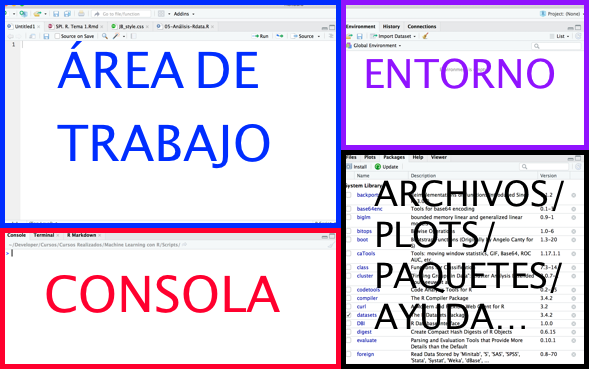
\includegraphics[width=0.9\linewidth]{Imgs/InterfazRStudio}
\end{frame}

\begin{frame}[fragile]{Cómo instalar RStudio}
\phantomsection\label{cuxf3mo-instalar-rstudio}
\begin{enumerate}
\tightlist
\item
  \href{http://www.rstudio.com/products/rstudio/download/}{Obtener
  RStudio}
\item
  \textbf{Solo si utilizáis Linux}, ejecutad en una terminal la
  siguiente instrucción para completar la instalación:
  \texttt{sudo\ dpkg\ -i\ rstudio-\textless{}version\textgreater{}-i386.deb},
  donde \texttt{version} refiere a la versión concreta que se haya
  descargado
\end{enumerate}

\begin{center}
\includegraphics[width=0.7\linewidth]{Imgs/RSLogo} \end{center}
\end{frame}

\begin{frame}{Trabajando con RStudio}
\phantomsection\label{trabajando-con-rstudio}
\begin{center}
\includegraphics[width=0.7\linewidth]{Imgs/easy_plus_tools} \end{center}
\end{frame}

\begin{frame}[fragile]{Cómo pedir ayuda}
\phantomsection\label{cuxf3mo-pedir-ayuda}
\begin{itemize}
\tightlist
\item
  \texttt{help()}: obtener ayuda por consola
\item
  \texttt{??...}: obtener ayuda por consola
\item
  Pestaña \texttt{Help} de Rstudio
\item
  \href{https://www.rstudio.com/wp-content/uploads/2015/02/rmarkdown-cheatsheet.pdf}{Cheat
  Sheet de RStudio} y
  \href{https://www.google.com/search?q=Cheat+Sheet++RStudio&rlz=1C1CHBF_esES891ES891&sxsrf=ALiCzsYTamg5AX36RN8EhpV8lSO55ijfRw\%3A1664221782651&ei=VgIyY5GzJ5nCa6rfovAP&ved=0ahUKEwiRtrqhnbP6AhUZ4RoKHaqvCP4Q4dUDCA4&uact=5&oq=Cheat+Sheet++RStudio&gs_lcp=Cgdnd3Mtd2l6EAMyCAgAEB4QBxATMggIABAeEAUQEzIICAAQHhAFEBMyCAgAEB4QBRATMggIABAeEAUQEzIICAAQHhAFEBMyCAgAEB4QBRATMggIABAeEAgQEzIICAAQHhAIEBMyCAgAEB4QCBATOgoIABBHENYEELADOggIABAeEAgQB0oECEEYAEoECEYYAFCmCljnC2DOEWgBcAF4AIABaogBzQGSAQMxLjGYAQCgAQHIAQjAAQE&sclient=gws-wiz}{más}
\item
  Buscad por la red (stackoverflow, R project\ldots)
\end{itemize}
\end{frame}

\begin{frame}[fragile]{Paquetes: cómo instalarlos y cargarlos}
\phantomsection\label{paquetes-cuxf3mo-instalarlos-y-cargarlos}
\blue{Paquete/librería}. Un \textbf{package} es una librería de
funciones y datos que que pueden venir o no instaladas en la carga de R
básico.

\begin{itemize}
\tightlist
\item
  \texttt{install.packages("nombre\_paquete",\ dep\ =\ TRUE)}: instala o
  actualiza un paquete de R
\item
  \texttt{library(nombre\_del\_paquete)}: carga un paquete ya instalado
\end{itemize}
\end{frame}

\section{Operaciones básicas}\label{operaciones-buxe1sicas}

\begin{frame}[fragile]{Operaciones}
\phantomsection\label{operaciones}
\begin{longtable}[]{@{}ll@{}}
\toprule\noalign{}
Código & Operación \\
\midrule\noalign{}
\endhead
\texttt{+} & Suma \\
\texttt{-} & Resta \\
\texttt{*} & Multiplicación \\
\texttt{/} & División \\
\texttt{\^{}} & Potencia \\
\texttt{\%/\%} & Cociente entero \\
\texttt{\%\%} & Resto de división entera \\
\bottomrule\noalign{}
\end{longtable}
\end{frame}

\begin{frame}[fragile]{Calculadora básica - Operaciones}
\phantomsection\label{calculadora-buxe1sica---operaciones}
\begin{longtable}[]{@{}ll@{}}
\toprule\noalign{}
Código & Significado \\
\midrule\noalign{}
\endhead
\texttt{pi} & {[}\(\pi\){]} \\
\texttt{Inf} &
\href{https://es.wikipedia.org/wiki/Infinito}{\(\infty\)} \\
\texttt{NaN} & Indeterminación (Not a Number) \\
\texttt{NA} & Valor desconocido (Not Available) \\
\bottomrule\noalign{}
\end{longtable}
\end{frame}

\begin{frame}[fragile]{Calculadora básica - Operaciones}
\phantomsection\label{calculadora-buxe1sica---operaciones-1}
\begin{Shaded}
\begin{Highlighting}[]
\DecValTok{2}\SpecialCharTok{+}\DecValTok{2}
\end{Highlighting}
\end{Shaded}

\begin{verbatim}
[1] 4
\end{verbatim}

\begin{Shaded}
\begin{Highlighting}[]
\DecValTok{77}\SpecialCharTok{\%/\%}\DecValTok{5}
\end{Highlighting}
\end{Shaded}

\begin{verbatim}
[1] 15
\end{verbatim}

\begin{Shaded}
\begin{Highlighting}[]
\DecValTok{77}\SpecialCharTok{\%\%}\DecValTok{5}
\end{Highlighting}
\end{Shaded}

\begin{verbatim}
[1] 2
\end{verbatim}
\end{frame}

\begin{frame}[fragile]{Funciones básicas}
\phantomsection\label{funciones-buxe1sicas}
\begin{longtable}[]{@{}ll@{}}
\toprule\noalign{}
Código & Función \\
\midrule\noalign{}
\endhead
\texttt{sqrt(x)} & \(\sqrt{x}\) \\
\texttt{exp(x)} & \(e^x\) \\
\texttt{log(x)} & \(\ln(x)\) \\
\texttt{log10(x)} & \(\log_{10}(x)\) \\
\texttt{log(x,a)} & \(\log_a(x)\) \\
\texttt{abs(x)} & \(\begin{vmatrix}x\end{vmatrix}\) \\
\bottomrule\noalign{}
\end{longtable}
\end{frame}

\begin{frame}[fragile]{Funciones básicas}
\phantomsection\label{funciones-buxe1sicas-1}
\begin{Shaded}
\begin{Highlighting}[]
\FunctionTok{sqrt}\NormalTok{(}\DecValTok{9}\NormalTok{)}
\end{Highlighting}
\end{Shaded}

\begin{verbatim}
[1] 3
\end{verbatim}

\begin{Shaded}
\begin{Highlighting}[]
\FunctionTok{log}\NormalTok{(}\FunctionTok{exp}\NormalTok{(}\DecValTok{1}\NormalTok{))}
\end{Highlighting}
\end{Shaded}

\begin{verbatim}
[1] 1
\end{verbatim}

\begin{Shaded}
\begin{Highlighting}[]
\FunctionTok{log}\NormalTok{(}\DecValTok{1000}\NormalTok{,}\DecValTok{10}\NormalTok{)}
\end{Highlighting}
\end{Shaded}

\begin{verbatim}
[1] 3
\end{verbatim}

\begin{Shaded}
\begin{Highlighting}[]
\FunctionTok{log10}\NormalTok{(}\DecValTok{1000}\NormalTok{)}
\end{Highlighting}
\end{Shaded}

\begin{verbatim}
[1] 3
\end{verbatim}
\end{frame}

\begin{frame}[fragile]{Combinatoria básica}
\phantomsection\label{combinatoria-buxe1sica}
\begin{longtable}[]{@{}ll@{}}
\toprule\noalign{}
Código & Operación \\
\midrule\noalign{}
\endhead
\texttt{factorial(x)} &
\href{https://es.wikipedia.org/wiki/Factorial}{x!} \\
\texttt{choose(n,m)} & \(\begin{pmatrix}n\\ m\end{pmatrix}\) \\
\bottomrule\noalign{}
\end{longtable}

\vspace{0.2cm}

\begin{itemize}
\item
  \blue{Número factorial.}

  Se define como número factorial de un número entero positivo \(n\)
  como \(n!=n\cdot(n-1)\cdots 2\cdot 1\)
\item
  \href{https://es.wikipedia.org/wiki/Coeficiente_binomial}{Coeficiente
  binomial}. Se define el coeficiente binomial de \(n\) sobre \(m\) como
  \[\begin{pmatrix}n\\ m\end{pmatrix}=\frac{n!}{m!(n-m)!}\]
\end{itemize}
\end{frame}

\begin{frame}[fragile]{Calculadora básica - Combinatoria}
\phantomsection\label{calculadora-buxe1sica---combinatoria}
\begin{Shaded}
\begin{Highlighting}[]
\FunctionTok{factorial}\NormalTok{(}\DecValTok{5}\NormalTok{)}
\end{Highlighting}
\end{Shaded}

\begin{verbatim}
[1] 120
\end{verbatim}

\begin{Shaded}
\begin{Highlighting}[]
\FunctionTok{choose}\NormalTok{(}\DecValTok{4}\NormalTok{,}\DecValTok{2}\NormalTok{)}
\end{Highlighting}
\end{Shaded}

\begin{verbatim}
[1] 6
\end{verbatim}

\begin{Shaded}
\begin{Highlighting}[]
\FunctionTok{factorial}\NormalTok{(}\DecValTok{6}\NormalTok{)}
\end{Highlighting}
\end{Shaded}

\begin{verbatim}
[1] 720
\end{verbatim}

\begin{Shaded}
\begin{Highlighting}[]
\FunctionTok{factorial}\NormalTok{(}\DecValTok{5}\NormalTok{)}\SpecialCharTok{*}\DecValTok{6}
\end{Highlighting}
\end{Shaded}

\begin{verbatim}
[1] 720
\end{verbatim}
\end{frame}

\begin{frame}[fragile]{Trigonometría en radianes}
\phantomsection\label{trigonometruxeda-en-radianes}
\begin{longtable}[]{@{}ll@{}}
\toprule\noalign{}
Código & Función \\
\midrule\noalign{}
\endhead
\texttt{sin(x)} & \(\sin(x)\) \\
\texttt{cos(x)} & \(\cos(x)\) \\
\texttt{tan(x)} & \(\tan(x)\) \\
\texttt{asin(x)} & \(\arcsin(x)\) \\
\texttt{acos(x)} & \(\arccos(x)\) \\
\texttt{atan(x)} & \(\arctan(x)\) \\
\bottomrule\noalign{}
\end{longtable}
\end{frame}

\begin{frame}[fragile]{Trigonometría en radianes}
\phantomsection\label{trigonometruxeda-en-radianes-1}
\begin{Shaded}
\begin{Highlighting}[]
\FunctionTok{sin}\NormalTok{(pi}\SpecialCharTok{/}\DecValTok{2}\NormalTok{)}
\end{Highlighting}
\end{Shaded}

\begin{verbatim}
[1] 1
\end{verbatim}

\begin{Shaded}
\begin{Highlighting}[]
\FunctionTok{cos}\NormalTok{(pi)}
\end{Highlighting}
\end{Shaded}

\begin{verbatim}
[1] -1
\end{verbatim}

\begin{Shaded}
\begin{Highlighting}[]
\FunctionTok{tan}\NormalTok{(}\DecValTok{0}\NormalTok{)}
\end{Highlighting}
\end{Shaded}

\begin{verbatim}
[1] 0
\end{verbatim}
\end{frame}

\begin{frame}[fragile]{Un ejemplo de gráficos}
\phantomsection\label{un-ejemplo-de-gruxe1ficos}
\begin{Shaded}
\begin{Highlighting}[]
\NormalTok{x }\OtherTok{=} \FunctionTok{seq}\NormalTok{(}\DecValTok{0}\NormalTok{,}\DecValTok{2}\SpecialCharTok{*}\NormalTok{pi,}\FloatTok{0.1}\NormalTok{)}
\FunctionTok{plot}\NormalTok{(x,}\FunctionTok{sin}\NormalTok{(x),}\AttributeTok{type=}\StringTok{"l"}\NormalTok{,}\AttributeTok{col=}\StringTok{"blue"}\NormalTok{,}\AttributeTok{lwd=}\DecValTok{3}\NormalTok{, }
     \AttributeTok{xlab=}\FunctionTok{expression}\NormalTok{(x), }\AttributeTok{ylab=}\StringTok{""}\NormalTok{,}
     \AttributeTok{xlim=}\FunctionTok{c}\NormalTok{(}\DecValTok{0}\NormalTok{,}\DecValTok{4}\NormalTok{),}\AttributeTok{cex=}\FloatTok{0.5}\NormalTok{)}
\FunctionTok{curve}\NormalTok{(}\FunctionTok{cos}\NormalTok{(x),}\AttributeTok{col=}\StringTok{"red"}\NormalTok{,}\AttributeTok{add=}\ConstantTok{TRUE}\NormalTok{)}
\FunctionTok{lines}\NormalTok{(x, }\FunctionTok{tan}\NormalTok{(x}\SpecialCharTok{/}\DecValTok{2}\NormalTok{), }\AttributeTok{col=}\StringTok{"purple"}\NormalTok{,}\AttributeTok{lwd=}\DecValTok{3}\NormalTok{)}
\FunctionTok{legend}\NormalTok{(}\StringTok{"bottomleft"}\NormalTok{,}
       \AttributeTok{col=}\FunctionTok{c}\NormalTok{(}\StringTok{"blue"}\NormalTok{,}\StringTok{"green"}\NormalTok{,}\StringTok{"purple"}\NormalTok{),}
       \AttributeTok{legend=}\FunctionTok{c}\NormalTok{(}\StringTok{"Seno"}\NormalTok{,}\StringTok{"Coseno"}\NormalTok{, }\StringTok{"Tangente"}\NormalTok{),}
       \AttributeTok{lwd=}\DecValTok{3}\NormalTok{, }\AttributeTok{bty=}\StringTok{"l"}\NormalTok{,}\AttributeTok{cex=}\FloatTok{0.8}\NormalTok{)}
\end{Highlighting}
\end{Shaded}
\end{frame}

\begin{frame}{Un ejemplo de gráficos}
\phantomsection\label{un-ejemplo-de-gruxe1ficos-1}
\ldots{} en tamaño normal

\begin{center}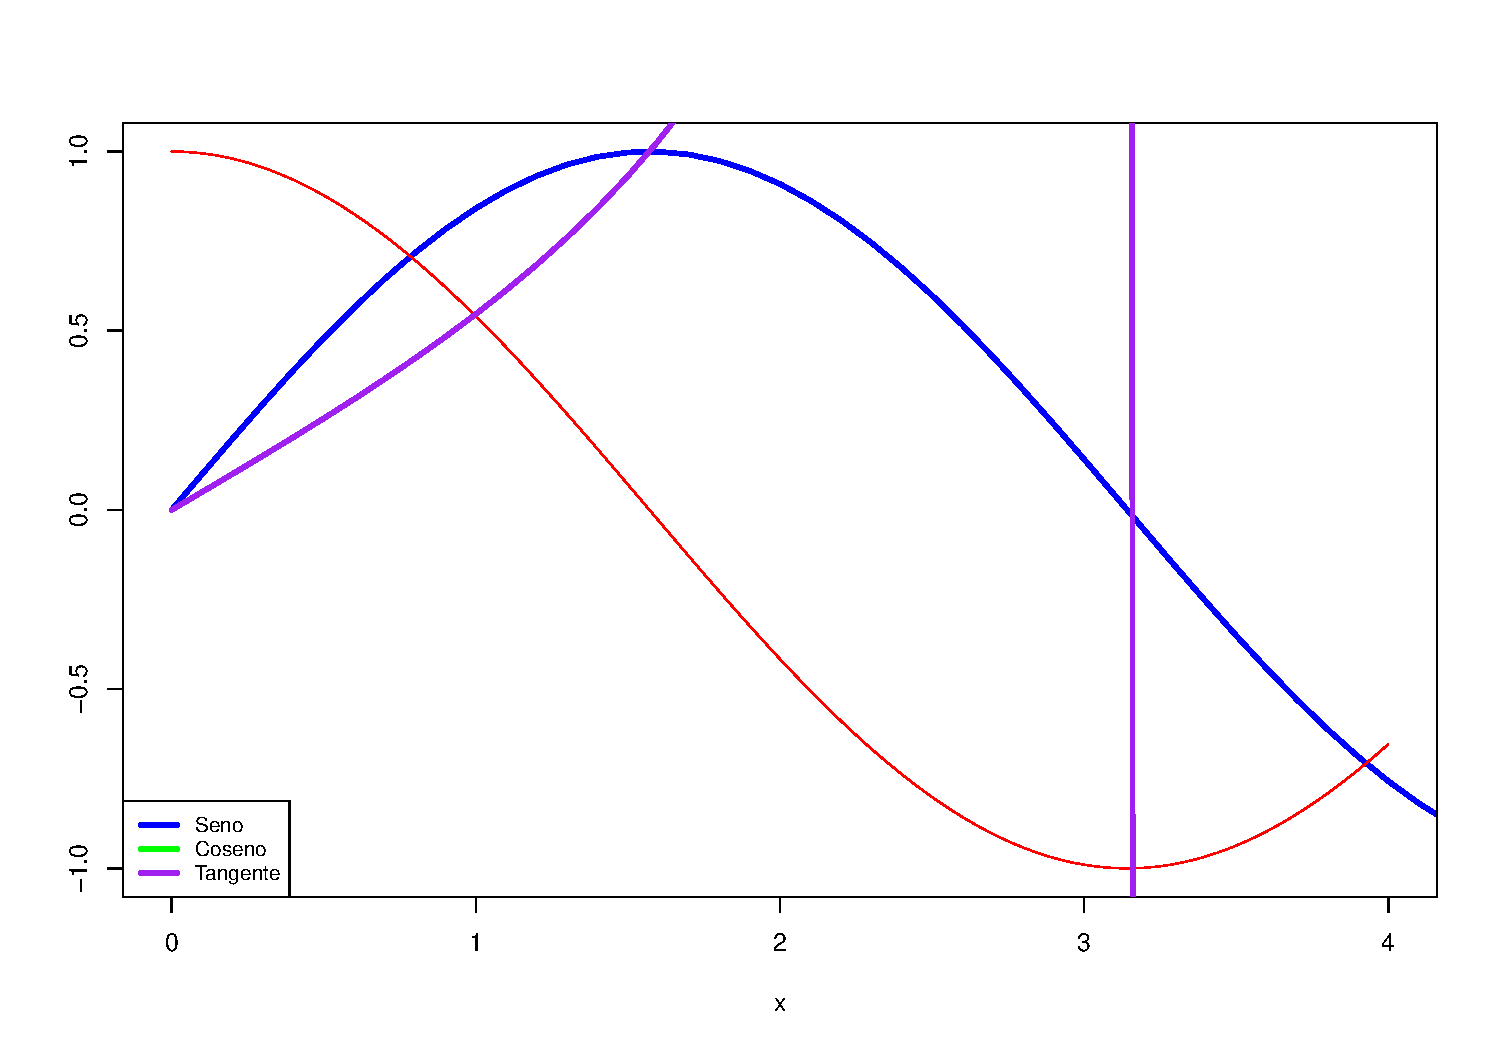
\includegraphics[width=0.8\linewidth]{R_base_files/figure-beamer/plot2_tema1-1} \end{center}
\end{frame}

\begin{frame}[fragile]{Números en coma flotante}
\phantomsection\label{nuxfameros-en-coma-flotante}
\begin{longtable}[]{@{}
  >{\raggedright\arraybackslash}p{(\columnwidth - 2\tabcolsep) * \real{0.2593}}
  >{\raggedright\arraybackslash}p{(\columnwidth - 2\tabcolsep) * \real{0.7407}}@{}}
\toprule\noalign{}
\begin{minipage}[b]{\linewidth}\raggedright
Código
\end{minipage} & \begin{minipage}[b]{\linewidth}\raggedright
Función
\end{minipage} \\
\midrule\noalign{}
\endhead
\texttt{print(x,n)} & Muestra las \(n\) cifras significativa del número
\(x\) \\
\texttt{round(x,n)} & Redondea a \(n\) cifras significativas un
resultado o vector numérico \(x\) \\
\texttt{floor(x)} & \(\lfloor x\rfloor\), parte entera por defecto de
\(x\) \\
\texttt{ceiling(x)} & \(\lceil x\rceil\), parte entera por exceso de
\(x\) \\
\texttt{trunc(x)} & Parte entera de \(x\), eliminando la parte
decimal \\
\bottomrule\noalign{}
\end{longtable}
\end{frame}

\begin{frame}[fragile]{Números en coma flotante}
\phantomsection\label{nuxfameros-en-coma-flotante-1}
\begin{Shaded}
\begin{Highlighting}[]
\FunctionTok{print}\NormalTok{(pi,}\DecValTok{5}\NormalTok{)}
\end{Highlighting}
\end{Shaded}

\begin{verbatim}
[1] 3.1416
\end{verbatim}

\begin{Shaded}
\begin{Highlighting}[]
\FunctionTok{round}\NormalTok{(pi,}\DecValTok{5}\NormalTok{)}
\end{Highlighting}
\end{Shaded}

\begin{verbatim}
[1] 3.14159
\end{verbatim}

\begin{Shaded}
\begin{Highlighting}[]
\FunctionTok{floor}\NormalTok{(pi)}
\end{Highlighting}
\end{Shaded}

\begin{verbatim}
[1] 3
\end{verbatim}

\begin{Shaded}
\begin{Highlighting}[]
\FunctionTok{ceiling}\NormalTok{(pi)}
\end{Highlighting}
\end{Shaded}

\begin{verbatim}
[1] 4
\end{verbatim}
\end{frame}

\begin{frame}[fragile]{Variables y funciones}
\phantomsection\label{variables-y-funciones}
\begin{itemize}
\tightlist
\item
  \texttt{nombre\_variable\ =\ valor}: define una variable con dicho
  valor
\item
  \texttt{nombre\_función\ =\ function(variable)\{función\}}: define una
  función
\end{itemize}

\begin{Shaded}
\begin{Highlighting}[]
\NormalTok{a}\OtherTok{=} \DecValTok{8}
\NormalTok{cubo }\OtherTok{=} \ControlFlowTok{function}\NormalTok{(x)\{x}\SpecialCharTok{\^{}}\DecValTok{3}\NormalTok{\}}
\FunctionTok{cubo}\NormalTok{(}\AttributeTok{x=}\NormalTok{a)}
\end{Highlighting}
\end{Shaded}

\begin{verbatim}
[1] 512
\end{verbatim}

\begin{Shaded}
\begin{Highlighting}[]
\NormalTok{raiz\_cúbica }\OtherTok{=} \ControlFlowTok{function}\NormalTok{(x)\{x}\SpecialCharTok{\^{}}\NormalTok{(}\DecValTok{1}\SpecialCharTok{/}\DecValTok{3}\NormalTok{)\}}
\NormalTok{raiz\_cúbica(a)}
\end{Highlighting}
\end{Shaded}

\begin{verbatim}
[1] 2
\end{verbatim}

\begin{Shaded}
\begin{Highlighting}[]
\NormalTok{raiz\_cúbica(}\FunctionTok{cubo}\NormalTok{(}\AttributeTok{x=}\NormalTok{a))}
\end{Highlighting}
\end{Shaded}

\begin{verbatim}
[1] 8
\end{verbatim}
\end{frame}

\section{Introducción}\label{introducciuxf3n}

\begin{frame}{Markdown}
\phantomsection\label{markdown}
\blue{R Markdown.} Es un tipo de fichero-programa en el cual podemos
intercalar sin problema alguno texto, código y fórmulas matemáticas.

Para la mayor parte de las necesidades de este curso, en lo referente a
la creación y composición de este tipo de ficheros, el documento
\emph{\href{https://en.support.wordpress.com/markdown-quick-reference/}{Markdown
Quick Reference} } y la
\href{http://shiny.rstudio.com/images/rm-cheatsheet.pdf.zip.}{chuleta}
de R Markdown deberían ser suficientes.

Sin embargo, a lo largo de este curso iremos ampliando estos contenidos
en algunos temas cuando lo creamos necesario.

Nosotros, en este tema, veremos cómo controlar el comportamiento de los
bloques de código (\blue{chunks}) al compilar el fichero R Markdown y
cómo escribir fórmulas matemáticas bien formateadas.
\end{frame}

\section{Fórmulas matemáticas}\label{fuxf3rmulas-matemuxe1ticas}

\begin{frame}{Cómo escribir}
\phantomsection\label{cuxf3mo-escribir}
Para escribir fórmulas matemáticas bien formateadas utilizaremos la
sintaxis \LaTeX

\begin{itemize}
\tightlist
\item
  Para tener ecuaciones o fórmulas en el mismo párrafo, escribimos
  nuestro código entre dos símbolos de dólar: código
\item
  Si queremos tener ecuaciones o fórmulas centradas en un párrafo
  aparte, escribimos nuestro código entre dos dobles símbolos de dólar:
  código
\end{itemize}

\red{¡Cuidado!} Al escribir una fórmula de la forma indicada
anteriormente o simplemente texto en R Markdown, los espacios en blanco
son completamente ignorados. RStudio solamente añade los espacios en
blanco a partir del significado lógico de sus elementos.
\end{frame}

\begin{frame}{Símbolos}
\phantomsection\label{suxedmbolos}
Hay muchísimos símbolos matemáticos que puedes escribirse con la
sintaxis \LaTeX. En el ejemplo anterior ya os hemos mostrado unos pocos.
En este tema, nosotros solo veremos los más utilizados.

Para quien quiera ir más allá, aquí os dejamos un
\href{http://www.ptep-online.com/ctan/symbols.pdf}{documento muy útil}
con gran cantidad de símbolos de \LaTeX.
\end{frame}

\begin{frame}[fragile]{Símbolos matemáticos - Básico}
\phantomsection\label{suxedmbolos-matemuxe1ticos---buxe1sico}
\begin{longtable}[]{@{}lll@{}}
\toprule\noalign{}
Significado & Código & Resultado \\
\midrule\noalign{}
\endhead
Suma & \texttt{+} & \(+\) \\
Resta & \texttt{-} & \(-\) \\
Producto & \texttt{\textbackslash{}cdot} & \(\cdot\) \\
Producto & \texttt{\textbackslash{}times} & \(\times\) \\
División & \texttt{\textbackslash{}div} & \(\div\) \\
Potencia & \texttt{a\^{}\{x\}} & \(a^{x}\) \\
Subíndice & \texttt{a\_\{i\}} & \(a_{i}\) \\
\bottomrule\noalign{}
\end{longtable}
\end{frame}

\begin{frame}[fragile]{Símbolos matemáticos - Básico}
\phantomsection\label{suxedmbolos-matemuxe1ticos---buxe1sico-1}
\begin{longtable}[]{@{}lll@{}}
\toprule\noalign{}
Significado & Código & Resultado \\
\midrule\noalign{}
\endhead
Fracción & \texttt{\textbackslash{}frac\{a\}\{b\}} & \(\frac{a}{b}\) \\
Más menos & \texttt{\textbackslash{}pm} & \(\pm\) \\
Raíz n-ésima & \texttt{\textbackslash{}sqrt{[}n{]}\{x\}} &
\(\sqrt[n]{x}\) \\
Unión & \texttt{cup} & \(\cup\) \\
Intersección & \texttt{\textbackslash{}cap} & \(\cap\) \\
OR lógico & \texttt{\textbackslash{}vee} & \(\vee\) \\
AND lógico & \texttt{\textbackslash{}wedge} & \(\wedge\) \\
\bottomrule\noalign{}
\end{longtable}
\end{frame}

\begin{frame}[fragile]{Símbolos matemáticos - Relaciones}
\phantomsection\label{suxedmbolos-matemuxe1ticos---relaciones}
\begin{longtable}[]{@{}lll@{}}
\toprule\noalign{}
Significado & Código & Resultado \\
\midrule\noalign{}
\endhead
Igual & \texttt{=} & \(=\) \\
Aproximado & \texttt{\textbackslash{}approx} & \(\approx\) \\
No igual & \texttt{\textbackslash{}ne} & \(\ne\) \\
Mayor que & \texttt{\textgreater{}} & \(>\) \\
Menor que & \texttt{\textless{}} & \(<\) \\
Mayor o igual que & \texttt{\textbackslash{}geq} & \(\geq\) \\
Menor o igual que & \texttt{\textbackslash{}leq} & \(\leq\) \\
\bottomrule\noalign{}
\end{longtable}
\end{frame}

\begin{frame}[fragile]{Símbolos matemáticos - Operadores}
\phantomsection\label{suxedmbolos-matemuxe1ticos---operadores}
\begin{longtable}[]{@{}lll@{}}
\toprule\noalign{}
Significado & Código & Resultado \\
\midrule\noalign{}
\endhead
Sumatorio & \texttt{\textbackslash{}sum\_\{i=0\}\^{}\{n\}} &
\(\sum_{i=0}^{n}\) \\
Productorio & \texttt{\textbackslash{}prod\_\{i=0\}\^{}\{n\}} &
\(\prod_{i=0}^{n}\) \\
Integral & \texttt{\textbackslash{}int\_\{a\}\^{}\{b\}} &
\(\int_{a}^{b}\) \\
Unión (grande) & \texttt{\textbackslash{}bigcup} & \(\bigcup\) \\
Intersección (grande) & \texttt{\textbackslash{}bigcap} & \(\bigcap\) \\
OR lógico (grande) & \texttt{\textbackslash{}bigvee} & \(\bigvee\) \\
AND lógico (grande) & \texttt{\textbackslash{}bigwedge} &
\(\bigwedge\) \\
\bottomrule\noalign{}
\end{longtable}
\end{frame}

\begin{frame}[fragile]{Símbolos matemáticos - Delimitadores}
\phantomsection\label{suxedmbolos-matemuxe1ticos---delimitadores}
\begin{longtable}[]{@{}lll@{}}
\toprule\noalign{}
Significado & Código & Resultado \\
\midrule\noalign{}
\endhead
Paréntesis & \texttt{()} & \((\ )\) \\
Corchetes & \texttt{{[}{]}} & \([\ ]\) \\
Llaves & \texttt{\textbackslash{}\{\ \textbackslash{}\}} & \(\{\ \}\) \\
Diamante & \texttt{\textbackslash{}langle\ \textbackslash{}rangle} &
\(\langle\ \rangle\) \\
Parte entera por defecto &
\texttt{\textbackslash{}lfloor\ \textbackslash{}rfloor} &
\(\lfloor\  \rfloor\) \\
Parte entera por exceso &
\texttt{\textbackslash{}lceil\ \textbackslash{}rceil} &
\(\lceil\ \rceil\) \\
Espacio en blanco & \texttt{hola\textbackslash{}\ caracola} &
\(hola\ caracola\) \\
\bottomrule\noalign{}
\end{longtable}
\end{frame}

\begin{frame}[fragile]{Símbolos matemáticos - Letras griegas}
\phantomsection\label{suxedmbolos-matemuxe1ticos---letras-griegas}
\begin{longtable}[]{@{}lll@{}}
\toprule\noalign{}
Significado & Código & Resultado \\
\midrule\noalign{}
\endhead
Alpha & \texttt{\textbackslash{}alpha} & \(\alpha\) \\
Beta & \texttt{\textbackslash{}beta} & \(\beta\) \\
Gamma & \texttt{\textbackslash{}gamma\ \textbackslash{}Gamma} &
\(\gamma\  \Gamma\) \\
Delta & \texttt{\textbackslash{}delta\ \textbackslash{}Delta} &
\(\delta\  \Delta\) \\
Epsilon & \texttt{\textbackslash{}epsilon} & \(\epsilon\) \\
Epsilon & \texttt{\textbackslash{}varepsilon} & \(\varepsilon\) \\
Zeta & \texttt{\textbackslash{}zeta} & \(\zeta\) \\
\bottomrule\noalign{}
\end{longtable}
\end{frame}

\begin{frame}[fragile]{Símbolos matemáticos - Letras griegas}
\phantomsection\label{suxedmbolos-matemuxe1ticos---letras-griegas-1}
\begin{longtable}[]{@{}lll@{}}
\toprule\noalign{}
Significado & Código & Resultado \\
\midrule\noalign{}
\endhead
Eta & \texttt{\textbackslash{}eta} & \(\eta\) \\
Theta & \texttt{\textbackslash{}theta\ \textbackslash{}Theta} &
\(\theta\ \Theta\) \\
Kappa & \texttt{\textbackslash{}kappa} & \(\kappa\) \\
Lambda & \texttt{\textbackslash{}lambda\ \textbackslash{}Lambda} &
\(\lambda\  \Lambda\) \\
Mu & \texttt{\textbackslash{}mu} & \(\mu\) \\
Nu & \texttt{\textbackslash{}nu} & \(\nu\) \\
Xi & \texttt{\textbackslash{}xi\ \textbackslash{}Xi} & \(\xi\ \Xi\) \\
\bottomrule\noalign{}
\end{longtable}
\end{frame}

\begin{frame}[fragile]{Símbolos matemáticos - Letras griegas}
\phantomsection\label{suxedmbolos-matemuxe1ticos---letras-griegas-2}
\begin{longtable}[]{@{}lll@{}}
\toprule\noalign{}
Significado & Código & Resultado \\
\midrule\noalign{}
\endhead
Pi & \texttt{\textbackslash{}pi\ \textbackslash{}Pi} & \(\pi\ \Pi\) \\
Rho & \texttt{\textbackslash{}rho} & \(\rho\) \\
Sigma & \texttt{\textbackslash{}sigma\ \textbackslash{}Sigma} &
\(\sigma\ \Sigma\) \\
Tau & \texttt{\textbackslash{}tau} & \(\tau\) \\
Upsilon & \texttt{\textbackslash{}upsilon\ \textbackslash{}Upsilon} &
\(\upsilon\ \Upsilon\) \\
Phi & \texttt{\textbackslash{}phi\ \textbackslash{}Phi} &
\(\phi\ \Phi\) \\
Phi & \texttt{\textbackslash{}varphi} & \(\varphi\) \\
\bottomrule\noalign{}
\end{longtable}
\end{frame}

\begin{frame}[fragile]{Símbolos matemáticos - Letras griegas}
\phantomsection\label{suxedmbolos-matemuxe1ticos---letras-griegas-3}
\begin{longtable}[]{@{}lll@{}}
\toprule\noalign{}
Significado & Código & Resultado \\
\midrule\noalign{}
\endhead
Chi & \texttt{\textbackslash{}chi} & \(\chi\) \\
Psi & \texttt{\textbackslash{}psi\ \textbackslash{}Psi} &
\(\psi\ \Psi\) \\
Omega & \texttt{\textbackslash{}omega\ \textbackslash{}Omega} &
\(\omega\ \Omega\) \\
\bottomrule\noalign{}
\end{longtable}
\end{frame}

\begin{frame}[fragile]{Símbolos matemáticos - Acentos matemáticos}
\phantomsection\label{suxedmbolos-matemuxe1ticos---acentos-matemuxe1ticos}
\begin{longtable}[]{@{}lll@{}}
\toprule\noalign{}
Significado & Código & Resultado \\
\midrule\noalign{}
\endhead
Gorrito & \texttt{\textbackslash{}hat\{x\}} & \(\hat{x}\) \\
Barra & \texttt{\textbackslash{}bar\{x\}} & \(\bar{x}\) \\
Punto 1 & \texttt{\textbackslash{}dot\{x\}} & \(\dot{x}\) \\
Punto 2 & \texttt{\textbackslash{}ddot\{x\}} & \(\ddot{x}\) \\
Punto 3 & \texttt{\textbackslash{}dddot\{x\}} & \(\dddot{x}\) \\
Tilde & \texttt{\textbackslash{}tilde\{x\}} & \(\tilde{x}\) \\
Vector & \texttt{\textbackslash{}vec\{x\}} & \(\vec{x}\) \\
\bottomrule\noalign{}
\end{longtable}
\end{frame}

\begin{frame}[fragile]{Símbolos matemáticos - Acentos expansibles}
\phantomsection\label{suxedmbolos-matemuxe1ticos---acentos-expansibles}
\begin{longtable}[]{@{}lll@{}}
\toprule\noalign{}
Significado & Código & Resultado \\
\midrule\noalign{}
\endhead
Gorrito & \texttt{\textbackslash{}widehat\{xyz\}} & \(\widehat{xyz}\) \\
Barra & \texttt{\textbackslash{}overline\{xyz\}} & \(\overline{xyz}\) \\
Subrallado & \texttt{\textbackslash{}underline\{xyz\}} &
\(\underline{xyz}\) \\
Llave superior & \texttt{\textbackslash{}overbrace\{xyz\}} &
\(\overbrace{xyz}\) \\
Llave inferior & \texttt{\textbackslash{}underbrace\{xyz\}} &
\(\underbrace{xyz}\) \\
Tilde & \texttt{\textbackslash{}widetilde\{xyz\}} &
\(\widetilde{xyz}\) \\
Vector & \texttt{\textbackslash{}overrightarrow\{xyz\}} &
\(\overrightarrow{xyz}\) \\
\bottomrule\noalign{}
\end{longtable}
\end{frame}

\begin{frame}[fragile]{Símbolos matemáticos - Flechas}
\phantomsection\label{suxedmbolos-matemuxe1ticos---flechas}
\begin{longtable}[]{@{}
  >{\raggedright\arraybackslash}p{(\columnwidth - 4\tabcolsep) * \real{0.3333}}
  >{\raggedright\arraybackslash}p{(\columnwidth - 4\tabcolsep) * \real{0.3333}}
  >{\raggedright\arraybackslash}p{(\columnwidth - 4\tabcolsep) * \real{0.3333}}@{}}
\toprule\noalign{}
\begin{minipage}[b]{\linewidth}\raggedright
Significado
\end{minipage} & \begin{minipage}[b]{\linewidth}\raggedright
Código
\end{minipage} & \begin{minipage}[b]{\linewidth}\raggedright
Resultado
\end{minipage} \\
\midrule\noalign{}
\endhead
Simple & \texttt{\textbackslash{}leftarrow\ \textbackslash{}rightarrow}
& \(\leftarrow\ \rightarrow\) \\
Doble & \texttt{\textbackslash{}Leftarrow\ \textbackslash{}Rightarrow} &
\(\Leftarrow\ \Rightarrow\) \\
Simple larga &
\texttt{\textbackslash{}longleftarrow\ \textbackslash{}longrightarrow} &
\(\longleftarrow\  \longrightarrow\) \\
Doble larga &
\texttt{\textbackslash{}Longleftarrow\ \textbackslash{}Longrightarrow} &
\(\Longleftarrow\ \Longrightarrow\) \\
Doble sentido simple & \texttt{\textbackslash{}leftrightarrow} &
\(\leftrightarrow\) \\
Doble sentido doble & \texttt{\textbackslash{}Leftrightarrow} &
\(\Leftrightarrow\) \\
\bottomrule\noalign{}
\end{longtable}
\end{frame}

\begin{frame}[fragile]{Símbolos matemáticos - Flechas}
\phantomsection\label{suxedmbolos-matemuxe1ticos---flechas-1}
\begin{longtable}[]{@{}
  >{\raggedright\arraybackslash}p{(\columnwidth - 4\tabcolsep) * \real{0.3333}}
  >{\raggedright\arraybackslash}p{(\columnwidth - 4\tabcolsep) * \real{0.3333}}
  >{\raggedright\arraybackslash}p{(\columnwidth - 4\tabcolsep) * \real{0.3333}}@{}}
\toprule\noalign{}
\begin{minipage}[b]{\linewidth}\raggedright
Significado
\end{minipage} & \begin{minipage}[b]{\linewidth}\raggedright
Código
\end{minipage} & \begin{minipage}[b]{\linewidth}\raggedright
Resultado
\end{minipage} \\
\midrule\noalign{}
\endhead
Doble sentido larga simple & \texttt{\textbackslash{}longleftrightarrow}
& \(\longleftrightarrow\) \\
Doble sentido larga doble & \texttt{\textbackslash{}Longleftrightarrow}
& \(\Longleftrightarrow\) \\
Mapea & \texttt{\textbackslash{}mapsto} & \(\mapsto\) \\
Arriba & \texttt{\textbackslash{}uparrow} & \(\uparrow\) \\
Abajo & \texttt{\textbackslash{}downarrow} & \(\downarrow\) \\
\bottomrule\noalign{}
\end{longtable}
\end{frame}

\begin{frame}[fragile]{Símbolos matemáticos - Funciones}
\phantomsection\label{suxedmbolos-matemuxe1ticos---funciones}
\begin{longtable}[]{@{}lll@{}}
\toprule\noalign{}
Significado & Código & Resultado \\
\midrule\noalign{}
\endhead
Seno & \texttt{\textbackslash{}sin} & \(\sin\) \\
Coseno & \texttt{\textbackslash{}cos} & \(\cos\) \\
Tangente & \texttt{\textbackslash{}tan} & \(\tan\) \\
Arcoseno & \texttt{\textbackslash{}arcsin} & \(\arcsin\) \\
Arcocoseno & \texttt{\textbackslash{}arccos} & \(\arccos\) \\
Arcotangente & \texttt{\textbackslash{}arctan} & \(\arctan\) \\
\bottomrule\noalign{}
\end{longtable}
\end{frame}

\begin{frame}[fragile]{Símbolos matemáticos - Funciones}
\phantomsection\label{suxedmbolos-matemuxe1ticos---funciones-1}
\begin{longtable}[]{@{}lll@{}}
\toprule\noalign{}
Significado & Código & Resultado \\
\midrule\noalign{}
\endhead
Exponencial & \texttt{\textbackslash{}exp} & \(\exp\) \\
Logaritmo & \texttt{\textbackslash{}log} & \(\log\) \\
Logaritmo neperiano & \texttt{\textbackslash{}ln} & \(\ln\) \\
Máximo & \texttt{\textbackslash{}max} & \(\max\) \\
Mínimo & \texttt{\textbackslash{}min} & \(\min\) \\
Límite & \texttt{\textbackslash{}lim} & \(\lim\) \\
\bottomrule\noalign{}
\end{longtable}
\end{frame}

\begin{frame}[fragile]{Símbolos matemáticos - Funciones}
\phantomsection\label{suxedmbolos-matemuxe1ticos---funciones-2}
\begin{longtable}[]{@{}lll@{}}
\toprule\noalign{}
Significado & Código & Resultado \\
\midrule\noalign{}
\endhead
Supremo & \texttt{\textbackslash{}sup} & \(\sup\) \\
Ínfimo & \texttt{\textbackslash{}inf} & \(\inf\) \\
Determinante & \texttt{\textbackslash{}det} & \(\det\) \\
Argumento & \texttt{\textbackslash{}arg} & \(\arg\) \\
\bottomrule\noalign{}
\end{longtable}
\end{frame}

\begin{frame}[fragile]{Símbolos matemáticos - Otros}
\phantomsection\label{suxedmbolos-matemuxe1ticos---otros}
\begin{longtable}[]{@{}lll@{}}
\toprule\noalign{}
Significado & Código & Resultado \\
\midrule\noalign{}
\endhead
Puntos suspensivos bajos & \texttt{\textbackslash{}ldots} &
\(\ldots\) \\
Puntos suspensivos centrados & \texttt{\textbackslash{}cdots} &
\(\cdots\) \\
Puntos suspensivos verticales & \texttt{\textbackslash{}vdots} &
\(\vdots\) \\
Puntos suspensivos diagonales & \texttt{\textbackslash{}ddots} &
\(\ddots\) \\
Cuantificador existencial & \texttt{\textbackslash{}exists} &
\(\exists\) \\
Cuantificador universal & \texttt{\textbackslash{}forall} &
\(\forall\) \\
Infinito & \texttt{\textbackslash{}infty} & \(\infty\) \\
\bottomrule\noalign{}
\end{longtable}
\end{frame}

\begin{frame}[fragile]{Símbolos matemáticos - Otros}
\phantomsection\label{suxedmbolos-matemuxe1ticos---otros-1}
\begin{longtable}[]{@{}lll@{}}
\toprule\noalign{}
Significado & Código & Resultado \\
\midrule\noalign{}
\endhead
Aleph & \texttt{\textbackslash{}aleph} & \(\aleph\) \\
Conjunto vacío & \texttt{\textbackslash{}emptyset} & \(\emptyset\) \\
Negación & \texttt{\textbackslash{}neg} & \(\neg\) \\
Barra invertida & \texttt{\textbackslash{}backslash} & \(\backslash\) \\
Dollar & \texttt{\textbackslash{}\$} & \(\$\) \\
Porcentaje & \texttt{\textbackslash{}\%} & \(\%\) \\
Parcial & \texttt{\textbackslash{}partial} & \(\partial\) \\
\bottomrule\noalign{}
\end{longtable}
\end{frame}

\begin{frame}[fragile]{Símbolos matemáticos - Tipos de letra}
\phantomsection\label{suxedmbolos-matemuxe1ticos---tipos-de-letra}
\begin{longtable}[]{@{}lll@{}}
\toprule\noalign{}
Significado & Código & Resultado \\
\midrule\noalign{}
\endhead
Negrita & \texttt{\textbackslash{}mathbf\{palabra\}} &
\(\mathbf{palabra}\) \\
Negrita & \texttt{\textbackslash{}boldsymbol\{palabra\}} &
\(\boldsymbol{palabra}\) \\
Negrita de pizarra & \texttt{\textbackslash{}mathbb\{NZQRC\}} &
\(\mathbb{NZQRC}\) \\
Caligráfica & \texttt{\textbackslash{}mathcal\{NZQRC\}} &
\(\mathcal{NZQRC}\) \\
Gótica & \texttt{\textbackslash{}mathfrak\{NZQRC\}} &
\(\mathfrak{NZQRC}\) \\
\bottomrule\noalign{}
\end{longtable}
\end{frame}

\begin{frame}[fragile]{Observaciones}
\phantomsection\label{observaciones}
\begin{itemize}
\item
  A la hora de componer en el interior de un párrafo una fracción,
  existen dos formas: adaptada al tamaño del
  texto,\texttt{\$\textbackslash{}frac\{a\}\{b\}\$}, que resulta en
  \(\frac{a}{b}\); o a tamaño real,
  \texttt{\$\textbackslash{}dfrac\{a\}\{b\}\$}, que da lugar a
  \(\dfrac{a}{b}\).
\item
  Podemos especificar que los delimitadores se adapten a la altura de la
  expresión que envuelven utilizando \texttt{\textbackslash{}left} y
  \texttt{\textbackslash{}right}. Observad el cambio en el siguiente
  ejemplo: \texttt{\$(\textbackslash{}dfrac\{a\}\{b\})\$} y
  \texttt{\$\textbackslash{}left(\textbackslash{}dfrac\{a\}\{b\}\textbackslash{}right)\$}
  producen, respectivamente \((\dfrac{a}{b})\) y
  \(\left(\dfrac{a}{b}\right)\).
\end{itemize}
\end{frame}

\begin{frame}[fragile]{Matrices}
\phantomsection\label{matrices}
\texttt{\$\$\textbackslash{}begin\{matrix\}\ a\_\{11\}\ \&\ a\_\{12\}\ \&\ a\_\{13\}\textbackslash{}\textbackslash{}\ a\_\{21\}\ \&\ a\_\{22\}\ \&\ a\_\{23\}\ \textbackslash{}end\{matrix\}\$\$}

\[\begin{matrix}
a_{11} & a_{12} & a_{13}\\
a_{21} & a_{22} & a_{23}
\end{matrix}\]

\texttt{\$\$\textbackslash{}begin\{pmatrix\}\ a\_\{11\}\ \&\ a\_\{12\}\ \&\ a\_\{13\}\textbackslash{}\textbackslash{}\ a\_\{21\}\ \&\ a\_\{22\}\ \&\ a\_\{23\}\ \textbackslash{}end\{pmatrix\}\$\$}

\[\begin{pmatrix}
a_{11} & a_{12} & a_{13}\\
a_{21} & a_{22} & a_{23}
\end{pmatrix}\]
\end{frame}

\begin{frame}[fragile]{Matrices}
\phantomsection\label{matrices-1}
\texttt{\$\$\textbackslash{}begin\{vmatrix\}\ a\_\{11\}\ \&\ a\_\{12\}\ \&\ a\_\{13\}\textbackslash{}\textbackslash{}\ a\_\{21\}\ \&\ a\_\{22\}\ \&\ a\_\{23\}\ \textbackslash{}end\{vmatrix\}\$\$}

\[\begin{vmatrix}
a_{11} & a_{12} & a_{13}\\
a_{21} & a_{22} & a_{23}
\end{vmatrix}\]

\texttt{\$\$\textbackslash{}begin\{bmatrix\}\ a\_\{11\}\ \&\ a\_\{12\}\ \&\ a\_\{13\}\textbackslash{}\textbackslash{}\ a\_\{21\}\ \&\ a\_\{22\}\ \&\ a\_\{23\}\ \textbackslash{}end\{bmatrix\}\$\$}

\[\begin{bmatrix}
a_{11} & a_{12} & a_{13}\\
a_{21} & a_{22} & a_{23}
\end{bmatrix}\]
\end{frame}

\begin{frame}[fragile]{Matrices}
\phantomsection\label{matrices-2}
\texttt{\$\$\textbackslash{}begin\{Bmatrix\}\ a\_\{11\}\ \&\ a\_\{12\}\ \&\ a\_\{13\}\textbackslash{}\textbackslash{}\ a\_\{21\}\ \&\ a\_\{22\}\ \&\ a\_\{23\}\ \textbackslash{}end\{Bmatrix\}\$\$}

\[\begin{Bmatrix}
a_{11} & a_{12} & a_{13}\\
a_{21} & a_{22} & a_{23}
\end{Bmatrix}\]

\texttt{\$\$\textbackslash{}begin\{Vmatrix\}\ a\_\{11\}\ \&\ a\_\{12\}\ \&\ a\_\{13\}\textbackslash{}\textbackslash{}\ a\_\{21\}\ \&\ a\_\{22\}\ \&\ a\_\{23\}\ \textbackslash{}end\{Vmatrix\}\$\$}

\[\begin{Vmatrix}
a_{11} & a_{12} & a_{13}\\
a_{21} & a_{22} & a_{23}
\end{Vmatrix}\]
\end{frame}

\begin{frame}[fragile]{Sistema de ecuaciones}
\phantomsection\label{sistema-de-ecuaciones}
\texttt{\textbackslash{}begin\{array\}\{ll\}\textbackslash{}end\{array\}}
nos produce una tabla alineada a la izquierda. El hecho de introducir el
código \texttt{\textbackslash{}left.\ \textbackslash{}right.} hace que
el delimitador respectivo no aparezca.

\begin{verbatim}
$$\left.\begin{array}{ll}
ax+by=& c\\
ex-fy=& g
\end{array}\right\}$$
\end{verbatim}

\[\left.\begin{array}{ll}
ax+by=& c\\
ex-fy=& g
\end{array}\right\}\]

\begin{verbatim}
$$|x|=\left\{\begin{array}{ll}
-x & \text{si }x\leq 0\\
x & \text{si }x\geq 0
\end{array}\right.
$$
\end{verbatim}

\[|x|=\left\{\begin{array}{ll}
-x & \text{si }x\leq 0\\
x & \text{si }x\geq 0
\end{array}\right.\]

La función de \LaTeX \texttt{\textbackslash{}text\{\}} nos permite
introducir texto en fórmulas matemáticas.
\end{frame}

\section{Parámetros de los chuncks de
R}\label{paruxe1metros-de-los-chuncks-de-r}

\begin{frame}[fragile]{Chunks de R}
\phantomsection\label{chunks-de-r}
\blue{Chunk.} Bloque de código.

Los bloques de código de R dentro de un documento R Markdown se indican
de la manera siguiente

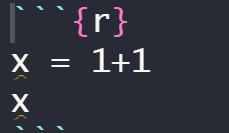
\includegraphics[width=0.15\linewidth]{Imgs/chunk_00}

que resulta en

\begin{Shaded}
\begin{Highlighting}[]
\NormalTok{x }\OtherTok{=} \DecValTok{1}\SpecialCharTok{+}\DecValTok{1}
\NormalTok{x}
\end{Highlighting}
\end{Shaded}
\end{frame}

\begin{frame}{Chunks de R}
\phantomsection\label{chunks-de-r-1}
Hay diversas opciones de crear un bloque de código de R:

\begin{itemize}
\tightlist
\item
  Ir al menú desplegable de ``Chunks'' y seleccionar el de R
\item
  Introducir manualmente
\item
  Alt + Command + I (para Mac) o Alt + Control + I (para Windows)
\end{itemize}
\end{frame}

\begin{frame}{Chunks de R}
\phantomsection\label{chunks-de-r-2}
A los chunks se les puede poner etiqueta, para así localizarlos de
manera más fácil. Por ejemplo

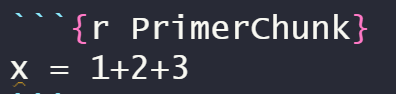
\includegraphics[width=0.6\linewidth]{Imgs/primer_chunk}

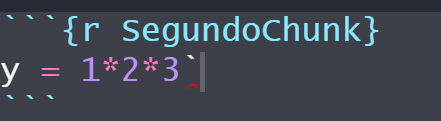
\includegraphics[width=0.6\linewidth]{Imgs/segundo_chunk}
\end{frame}

\begin{frame}[fragile]{Parámetros de los chunks}
\phantomsection\label{paruxe1metros-de-los-chunks}
La parte entre llaves también puede contener diversos parámetros,
separados por comas entre ellos y separados de la etiqueta (o de r, si
hemos decidido no poner ninguna).

Estos parámetros determinan el comportamiento del bloque al compilar el
documento pulsando el botón \texttt{Knit} situado en la barra superior
del área de trabajo.
\end{frame}

\begin{frame}[fragile]{Parámetros de los chunks}
\phantomsection\label{paruxe1metros-de-los-chunks-1}
\begin{longtable}[]{@{}
  >{\raggedright\arraybackslash}p{(\columnwidth - 2\tabcolsep) * \real{0.5000}}
  >{\raggedright\arraybackslash}p{(\columnwidth - 2\tabcolsep) * \real{0.5000}}@{}}
\toprule\noalign{}
\begin{minipage}[b]{\linewidth}\raggedright
Código
\end{minipage} & \begin{minipage}[b]{\linewidth}\raggedright
Significado
\end{minipage} \\
\midrule\noalign{}
\endhead
\texttt{echo} & Si lo igualamos a \texttt{TRUE}, que es el valor por
defecto, estaremos diciendo que queremos que se muestre el código fuente
del chunk. En cambio, igualado a \texttt{FALSE}, no se mostrará \\
\texttt{eval} & Si lo igualamos a \texttt{TRUE}, que es el valor por
defecto, estaremos diciendo que queremos que se evalúe el código. En
cambio, igualado a \texttt{FALSE}, no se evaluará \\
\bottomrule\noalign{}
\end{longtable}
\end{frame}

\begin{frame}[fragile]{Parámetros de los chunks}
\phantomsection\label{paruxe1metros-de-los-chunks-2}
\begin{longtable}[]{@{}
  >{\raggedright\arraybackslash}p{(\columnwidth - 2\tabcolsep) * \real{0.5000}}
  >{\raggedright\arraybackslash}p{(\columnwidth - 2\tabcolsep) * \real{0.5000}}@{}}
\toprule\noalign{}
\begin{minipage}[b]{\linewidth}\raggedright
Código
\end{minipage} & \begin{minipage}[b]{\linewidth}\raggedright
Significado
\end{minipage} \\
\midrule\noalign{}
\endhead
\texttt{message} & Nos permite indicar si queremos que se muestren los
mensajes que R produce al ejecutar código. Igualado a \texttt{TRUE} se
muestran, igualado a \texttt{FALSE} no \\
\texttt{warning} & Nos permite indicar si queremos que se muestren los
mensajes de advertencia que producen algunas funciones al ejecutarse.
Igualado a \texttt{TRUE} se muestran, igualado a \texttt{FALSE} no \\
\bottomrule\noalign{}
\end{longtable}
\end{frame}

\begin{frame}[fragile]{Parámetros de los chunks}
\phantomsection\label{paruxe1metros-de-los-chunks-3}
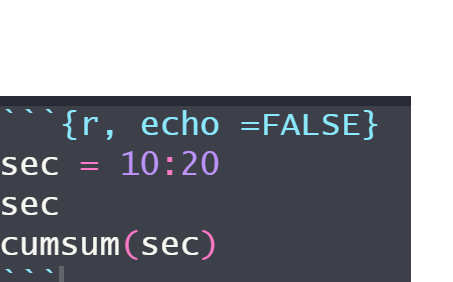
\includegraphics[width=0.5\linewidth]{Imgs/no_aparece}

No aparece el código solo la salida

\begin{verbatim}
 [1] 10 11 12 13 14 15 16 17 18 19 20
\end{verbatim}

\begin{verbatim}
 [1]  10  21  33  46  60  75  91 108 126 145 165
\end{verbatim}
\end{frame}

\begin{frame}[fragile]{Parámetros de los chunks}
\phantomsection\label{paruxe1metros-de-los-chunks-4}
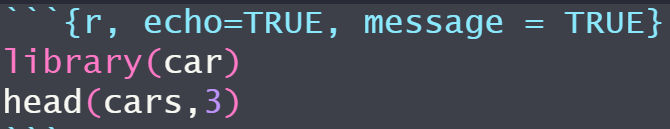
\includegraphics[width=0.6\linewidth]{Imgs/parametros_chunk_2}

\begin{Shaded}
\begin{Highlighting}[]
\FunctionTok{library}\NormalTok{(car)}
\end{Highlighting}
\end{Shaded}

\begin{verbatim}
Cargando paquete requerido: carData
\end{verbatim}

\begin{Shaded}
\begin{Highlighting}[]
\FunctionTok{head}\NormalTok{(cars,}\DecValTok{3}\NormalTok{)}
\end{Highlighting}
\end{Shaded}

\begin{verbatim}
  speed dist
1     4    2
2     4   10
3     7    4
\end{verbatim}
\end{frame}

\begin{frame}[fragile]{Parámetros de los chunks}
\phantomsection\label{paruxe1metros-de-los-chunks-5}
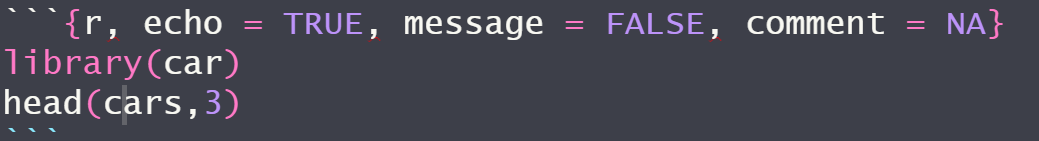
\includegraphics[width=0.6\linewidth]{Imgs/para_chunks_3}

\begin{Shaded}
\begin{Highlighting}[]
\FunctionTok{library}\NormalTok{(car)}
\FunctionTok{head}\NormalTok{(cars,}\DecValTok{3}\NormalTok{)}
\end{Highlighting}
\end{Shaded}

\begin{verbatim}
  speed dist
1     4    2
2     4   10
3     7    4
\end{verbatim}

Fijaos que \texttt{comment=NA} evita que aparezcan los \texttt{\#\#}
\end{frame}

\begin{frame}[fragile]{Parámetros de los chunks}
\phantomsection\label{paruxe1metros-de-los-chunks-6}
\begin{longtable}[]{@{}
  >{\raggedright\arraybackslash}p{(\columnwidth - 4\tabcolsep) * \real{0.3333}}
  >{\raggedright\arraybackslash}p{(\columnwidth - 4\tabcolsep) * \real{0.3333}}
  >{\raggedright\arraybackslash}p{(\columnwidth - 4\tabcolsep) * \real{0.3333}}@{}}
\toprule\noalign{}
\begin{minipage}[b]{\linewidth}\raggedright
Significado
\end{minipage} & \begin{minipage}[b]{\linewidth}\raggedright
Código
\end{minipage} & \begin{minipage}[b]{\linewidth}\raggedright
Resultado
\end{minipage} \\
\midrule\noalign{}
\endhead
\texttt{results} & \texttt{markup} & Valor por defecto. Nos muestra los
resultados en el documento final línea a línea, encabezados por
\texttt{\#\#} \\
\texttt{results} & \texttt{hide} & No se nos muestra el resultado en el
documento final \\
\texttt{results} & \texttt{asis} & Nos devuelve los resultados línea a
línea de manera literal en el documento final y el programa con el que
se abre el documento final los interpreta como texto y formatea
adecuadamente \\
\texttt{results} & \texttt{hold} & Miestra todos los resultados al final
del bloque de código \\
\bottomrule\noalign{}
\end{longtable}
\end{frame}

\begin{frame}[fragile]{Parámetros de los chunks}
\phantomsection\label{paruxe1metros-de-los-chunks-7}
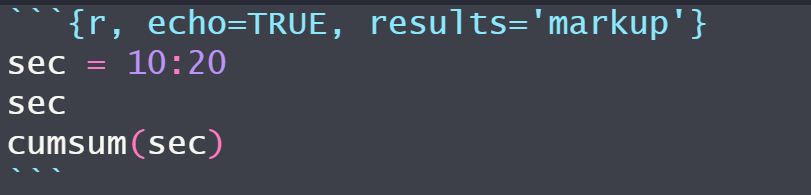
\includegraphics[width=0.6\linewidth]{Imgs/para_chunks_03}

\begin{Shaded}
\begin{Highlighting}[]
\NormalTok{sec }\OtherTok{=} \DecValTok{10}\SpecialCharTok{:}\DecValTok{20}
\NormalTok{sec}
\end{Highlighting}
\end{Shaded}

\begin{verbatim}
 [1] 10 11 12 13 14 15 16 17 18 19 20
\end{verbatim}

\begin{Shaded}
\begin{Highlighting}[]
\FunctionTok{cumsum}\NormalTok{(sec)}
\end{Highlighting}
\end{Shaded}

\begin{verbatim}
 [1]  10  21  33  46  60  75  91 108 126 145 165
\end{verbatim}
\end{frame}

\begin{frame}[fragile]{Parámetros de los chunks}
\phantomsection\label{paruxe1metros-de-los-chunks-8}
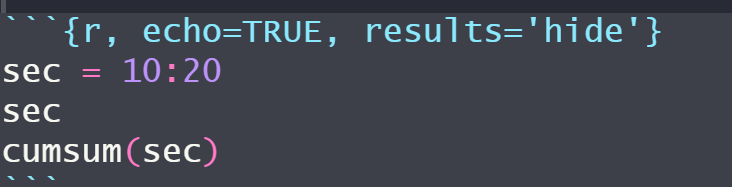
\includegraphics[width=0.6\linewidth]{Imgs/parametros_chunk_4}

\begin{Shaded}
\begin{Highlighting}[]
\NormalTok{sec }\OtherTok{=} \DecValTok{10}\SpecialCharTok{:}\DecValTok{20}
\NormalTok{sec}
\FunctionTok{cumsum}\NormalTok{(sec)}
\end{Highlighting}
\end{Shaded}
\end{frame}

\begin{frame}[fragile]{Parámetros de los chunks}
\phantomsection\label{paruxe1metros-de-los-chunks-9}
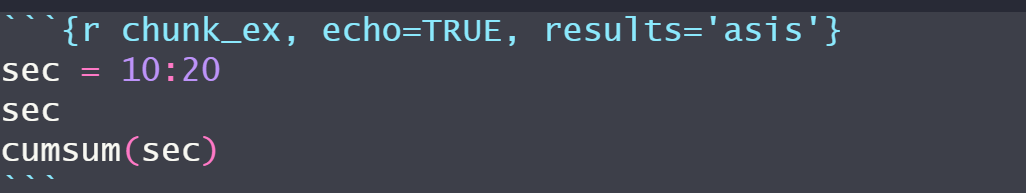
\includegraphics[width=0.6\linewidth]{Imgs/parametros_chunk_5}

\begin{Shaded}
\begin{Highlighting}[]
\NormalTok{sec }\OtherTok{=} \DecValTok{10}\SpecialCharTok{:}\DecValTok{20}
\NormalTok{sec}
\end{Highlighting}
\end{Shaded}

{[}1{]} 10 11 12 13 14 15 16 17 18 19 20

\begin{Shaded}
\begin{Highlighting}[]
\FunctionTok{cumsum}\NormalTok{(sec)}
\end{Highlighting}
\end{Shaded}

{[}1{]} 10 21 33 46 60 75 91 108 126 145 165
\end{frame}

\begin{frame}[fragile]{Parámetros de los chunks}
\phantomsection\label{paruxe1metros-de-los-chunks-10}
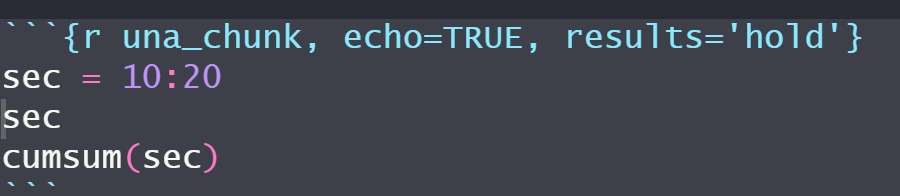
\includegraphics[width=0.6\linewidth]{Imgs/parametros_chunk_6}

\begin{Shaded}
\begin{Highlighting}[]
\NormalTok{sec }\OtherTok{=} \DecValTok{10}\SpecialCharTok{:}\DecValTok{20}
\NormalTok{sec}
\FunctionTok{cumsum}\NormalTok{(sec)}
\end{Highlighting}
\end{Shaded}

\begin{verbatim}
 [1] 10 11 12 13 14 15 16 17 18 19 20
 [1]  10  21  33  46  60  75  91 108 126 145 165
\end{verbatim}
\end{frame}

\section{Estructuras de datos}\label{estructuras-de-datos}

\begin{frame}[fragile]{Tipos de datos en R, vectores}
\phantomsection\label{tipos-de-datos-en-r-vectores}
Un \textbf{vector} es una secuencia ordenada de datos. \texttt{R}
dispone de muchos tipos de datos, por ejemplo:

\begin{itemize}
\tightlist
\item
  \texttt{logical}: lógicos (\texttt{TRUE} o \texttt{FALSE})
\item
  \texttt{integer}: números enteros, \(\mathbb Z\)
\item
  \texttt{numeric}: números reales, \(\mathbb R\)
\item
  \texttt{complex}: números complejos, \(\mathbb C\)
\item
  \texttt{character}: palabras
\end{itemize}

En los vectores de \texttt{R}, todos sus objetos han de ser del mismo
tipo: todos números, todos palabras, etc. Cuando queramos usar vectores
formados por objetos de diferentes tipos, tendremos que usar
\textbf{listas generalizadas}, \texttt{lists} que veremos al final del
tema.
\end{frame}

\begin{frame}[fragile]{Básico}
\phantomsection\label{buxe1sico}
\begin{itemize}
\tightlist
\item
  \texttt{c()}: para definir un vector
\item
  \texttt{scan()}: para definir un vector
\item
  \texttt{fix(x)}: para modificar visualmente el vector \(x\)
\item
  \texttt{rep(a,n)}: para definir un vector constante que contiene el
  dato \(a\) repetido \(n\) veces
\end{itemize}

\begin{Shaded}
\begin{Highlighting}[]
\FunctionTok{c}\NormalTok{(}\DecValTok{1}\NormalTok{,}\DecValTok{2}\NormalTok{,}\DecValTok{3}\NormalTok{)}
\end{Highlighting}
\end{Shaded}

\begin{verbatim}
[1] 1 2 3
\end{verbatim}

\begin{Shaded}
\begin{Highlighting}[]
\FunctionTok{rep}\NormalTok{(}\StringTok{"Mates"}\NormalTok{,}\DecValTok{7}\NormalTok{)}
\end{Highlighting}
\end{Shaded}

\begin{verbatim}
[1] "Mates" "Mates" "Mates" "Mates" "Mates" "Mates" "Mates"
\end{verbatim}
\end{frame}

\begin{frame}{Función scan()}
\phantomsection\label{funciuxf3n-scan}
\textbf{Ejemplo}

Vamos a crear un vector que contenga 3 copias de 1 9 9 8 0 7 2 6 con la
función scan:

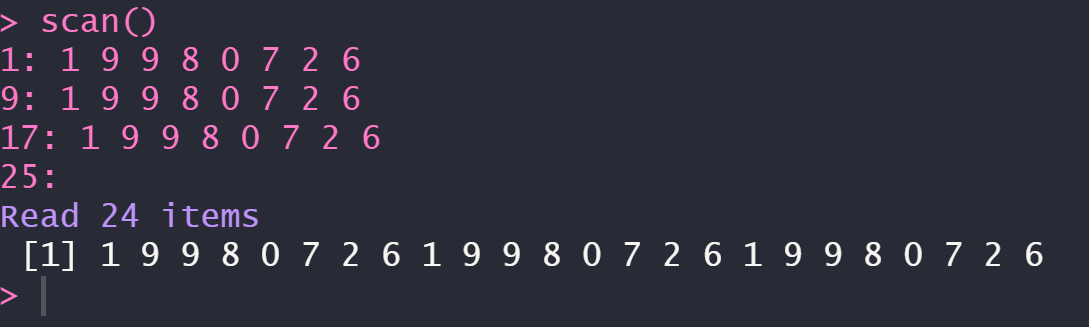
\includegraphics[width=0.6\linewidth]{Imgs/scan}
\end{frame}

\begin{frame}{Básico}
\phantomsection\label{buxe1sico-1}
\textbf{Ejercicio}

\begin{enumerate}
\item
  Repite tu año de nacimiento 10 veces
\item
  Crea el vector que tenga como entradas
  \(16, 0, 1, 20, 1, 7, 88, 5, 1, 9\), llámalo vec y modifica la cuarta
  entrada con la función fix()
\end{enumerate}
\end{frame}

\begin{frame}[fragile]{Progresiones y Secuencias}
\phantomsection\label{progresiones-y-secuencias}
Una progresión aritmética es una sucesión de números tales que la
\textbf{diferencia}, \(d\), de cualquier par de términos sucesivos de la
secuencia es constante. \[a_n = a_1 + (n-1)\cdot d\]

\begin{itemize}
\tightlist
\item
  \texttt{seq(a,b,by=d)}: para generar una
  \href{https://es.wikipedia.org/wiki/Progresión_aritmética}{progresión
  aritmética} de diferencia \(d\) que empieza en \(a\) hasta llegar a
  \(b\)
\item
  \texttt{seq(a,b,\ length.out=n)}: define progresión aritmética de
  longitud \(n\) que va de \(a\) a \(b\) con diferencia \(d\). Por tanto
  \(d=(b-a)/(n-1)\)
\item
  \texttt{seq(a,by=d,\ length.out=n)}: define la progresión aritmética
  de longitud \(n\) y diferencia \(d\) que empieza en \(a\)
\item
  \texttt{a:b}: define la secuencia de números \textbf{enteros}
  (\(\mathbb{Z}\)) consecutivos entre dos números \(a\) y \(b\)
\end{itemize}
\end{frame}

\begin{frame}{Secuencias}
\phantomsection\label{secuencias}
\textbf{Ejercicio}

\begin{itemize}
\item
  Imprimid los números del 1 al 20
\item
  Imprimid los 20 primeros números pares
\item
  Imprimid 30 números equidistantes entre el 17 y el 98, mostrando solo
  4 cifras significativas
\end{itemize}
\end{frame}

\begin{frame}[fragile]{Funciones}
\phantomsection\label{funciones}
Cuando queremos aplicar una función a cada uno de los elementos de un
vector de datos, la función \texttt{sapply} nos ahorra tener que
programar con bucles en \texttt{R}:

\begin{itemize}
\tightlist
\item
  \texttt{sapply(nombre\_de\_vector,FUN=nombre\_de\_función)}: para
  aplicar dicha función a todos los elementos del vector
\item
  \texttt{sqrt(x)}: calcula un nuevo vector con las raíces cuadradas de
  cada uno de los elementos del vector \(x\)
\end{itemize}
\end{frame}

\begin{frame}[fragile]{Funciones}
\phantomsection\label{funciones-1}
Dado un vector de datos \(x\) podemos calcular muchas medidas
estadísticas acerca del mismo:

\begin{itemize}
\tightlist
\item
  \texttt{length(x)}: calcula la longitud del vector \(x\)
\item
  \texttt{max(x)}: calcula el máximo del vector \(x\)
\item
  \texttt{min(x)}: calcula el mínimo del vector \(x\)
\item
  \texttt{sum(x)}: calcula la suma de las entradas del vector \(x\)
\item
  \texttt{prod(x)}: calcula el producto de las entradas del vector \(x\)
\end{itemize}
\end{frame}

\begin{frame}[fragile]{Funciones}
\phantomsection\label{funciones-2}
\begin{itemize}
\tightlist
\item
  \texttt{mean(x)}: calcula la media aritmética de las entradas del
  vector \(x\)
\item
  \texttt{diff(x)}: calcula el vector formado por las diferencias
  sucesivas entre entradas del vector original \(x\)
\item
  \texttt{cumsum(x)}: calcula el vector formado por las sumas acumuladas
  de las entradas del vector original \(x\)

  \begin{itemize}
  \tightlist
  \item
    Permite definir sucesiones descritas mediante sumatorios
  \item
    Cada entrada de \texttt{cumsum(x)} es la suma de las entradas de
    \(x\) hasta su posición
  \end{itemize}
\end{itemize}
\end{frame}

\begin{frame}[fragile]{Funciones}
\phantomsection\label{funciones-3}
\begin{Shaded}
\begin{Highlighting}[]
\NormalTok{cuadrado }\OtherTok{=} \ControlFlowTok{function}\NormalTok{(x)\{x}\SpecialCharTok{\^{}}\DecValTok{2}\NormalTok{\}}
\NormalTok{v }\OtherTok{=} \FunctionTok{c}\NormalTok{(}\DecValTok{1}\NormalTok{,}\DecValTok{2}\NormalTok{,}\DecValTok{3}\NormalTok{,}\DecValTok{4}\NormalTok{,}\DecValTok{5}\NormalTok{,}\DecValTok{6}\NormalTok{)}
\FunctionTok{sapply}\NormalTok{(v, }\AttributeTok{FUN =}\NormalTok{ cuadrado)}
\end{Highlighting}
\end{Shaded}

\begin{verbatim}
[1]  1  4  9 16 25 36
\end{verbatim}

\begin{Shaded}
\begin{Highlighting}[]
\FunctionTok{mean}\NormalTok{(v)}
\end{Highlighting}
\end{Shaded}

\begin{verbatim}
[1] 3.5
\end{verbatim}

\begin{Shaded}
\begin{Highlighting}[]
\FunctionTok{cumsum}\NormalTok{(v)}
\end{Highlighting}
\end{Shaded}

\begin{verbatim}
[1]  1  3  6 10 15 21
\end{verbatim}
\end{frame}

\begin{frame}[fragile]{Orden}
\phantomsection\label{orden}
\begin{itemize}
\tightlist
\item
  \texttt{sort(x)}: ordena el vector en orden natural de los objetos que
  lo forman: el orden numérico creciente, orden alfabético\ldots{}
\item
  \texttt{rev(x)}: invierte el orden de los elementos del vector \(x\)
\end{itemize}

\begin{Shaded}
\begin{Highlighting}[]
\NormalTok{v }\OtherTok{=} \FunctionTok{c}\NormalTok{(}\DecValTok{1}\NormalTok{,}\DecValTok{7}\NormalTok{,}\DecValTok{5}\NormalTok{,}\DecValTok{2}\NormalTok{,}\DecValTok{4}\NormalTok{,}\DecValTok{6}\NormalTok{,}\DecValTok{3}\NormalTok{)}
\FunctionTok{sort}\NormalTok{(v)}
\end{Highlighting}
\end{Shaded}

\begin{verbatim}
[1] 1 2 3 4 5 6 7
\end{verbatim}

\begin{Shaded}
\begin{Highlighting}[]
\FunctionTok{rev}\NormalTok{(v)}
\end{Highlighting}
\end{Shaded}

\begin{verbatim}
[1] 3 6 4 2 5 7 1
\end{verbatim}
\end{frame}

\begin{frame}[fragile]{Orden}
\phantomsection\label{orden-1}
\textbf{Ejercicio}

\begin{itemize}
\item
  Combinad las dos funciones anteriores, \texttt{sort} y \texttt{rev}
  para crear una función que dado un vector \(x\) os lo devuelva
  ordenado en orden decreciente.
\item
  Razonad si aplicar primero \texttt{sort} y luego \texttt{rev} a un
  vector \(x\) daría en general el mismo resultado que aplicar primero
  \texttt{rev} y luego \texttt{sort}.
\item
  Investigad la documentación de la función \texttt{sort} (recordad que
  podéis usar la sintaxis \texttt{?sort} en la consola) para leer si
  cambiando algún argumento de la misma podéis obtener el mismo
  resultado que habéis programado en el primer ejercicio.
\end{itemize}
\end{frame}

\begin{frame}[fragile]{Subvectores}
\phantomsection\label{subvectores}
\begin{itemize}
\item
  \texttt{vector{[}i{]}}: da la \(i\)-ésima entrada del vector

  \begin{itemize}
  \tightlist
  \item
    Los índices en R empiezan en 1
  \item
    \texttt{vector{[}length(vector){]}}: nos da la última entrada del
    vector
  \item
    \texttt{vector{[}a:b{]}}: si \(a\) y \(b\) son dos números
    naturales, nos da el subvector con las entradas del vector original
    que van de la posición \(a\)-ésima hasta la \(b\)-ésima.
  \item
    \texttt{vector{[}-i{]}}: si \(i\) es un número, este subvector está
    formado por todas las entradas del vector original menos la entrada
    \(i\)-ésima. Si \(i\) resulta ser un vector, entonces es un vector
    de índices y crea un nuevo vector con las entradas del vector
    original,cuyos índices pertenecen a \(i\)
  \item
    \texttt{vector{[}-x{]}}: si \(x\) es un vector (de índices),
    entonces este es el complementario de vector{[}\(x\){]}
  \end{itemize}
\end{itemize}
\end{frame}

\begin{frame}[fragile]{Subvectores}
\phantomsection\label{subvectores-1}
\begin{itemize}
\item
  También podemos utilizar operadores lógicos:

  \begin{itemize}
  \tightlist
  \item
    \texttt{==}: =
  \item
    \texttt{!=}: \(\neq\)
  \item
    \texttt{\textgreater{}=}: \(\ge\)\\
  \item
    \texttt{\textless{}=}: \(\le\)
  \item
    \texttt{\textless{}}: \(<\)
  \item
    \texttt{\textgreater{}}: \(>\)
  \item
    \texttt{!}: NO lógico
  \item
    \texttt{\&}: Y lógico
  \item
    \texttt{\textbar{}}: O lógico
  \end{itemize}
\end{itemize}
\end{frame}

\begin{frame}[fragile]{Subvectores}
\phantomsection\label{subvectores-2}
\begin{Shaded}
\begin{Highlighting}[]
\NormalTok{v }\OtherTok{=} \FunctionTok{c}\NormalTok{(}\DecValTok{14}\NormalTok{,}\DecValTok{5}\NormalTok{,}\DecValTok{6}\NormalTok{,}\DecValTok{19}\NormalTok{,}\DecValTok{32}\NormalTok{,}\DecValTok{0}\NormalTok{,}\DecValTok{8}\NormalTok{)}
\NormalTok{v[}\DecValTok{2}\NormalTok{]}
\end{Highlighting}
\end{Shaded}

\begin{verbatim}
[1] 5
\end{verbatim}

\begin{Shaded}
\begin{Highlighting}[]
\NormalTok{v[}\SpecialCharTok{{-}}\FunctionTok{c}\NormalTok{(}\DecValTok{3}\NormalTok{,}\DecValTok{5}\NormalTok{)]}
\end{Highlighting}
\end{Shaded}

\begin{verbatim}
[1] 14  5 19  0  8
\end{verbatim}

\begin{Shaded}
\begin{Highlighting}[]
\NormalTok{v[v }\SpecialCharTok{!=} \DecValTok{19} \SpecialCharTok{\&}\NormalTok{ v}\SpecialCharTok{\textgreater{}}\DecValTok{15}\NormalTok{]}
\end{Highlighting}
\end{Shaded}

\begin{verbatim}
[1] 32
\end{verbatim}
\end{frame}

\begin{frame}[fragile]{Condicionales}
\phantomsection\label{condicionales}
\begin{itemize}
\tightlist
\item
  \texttt{which(x\ cumple\ condición)}: para obtener los índices de las
  entradas del vector \(x\) que satisfacen la condición dada
\item
  \texttt{which.min(x)}: nos da la primera posición en la que el vector
  \(x\) toma su valor mínimo
\item
  \texttt{which(x==min(x))}: da todas las posiciones en las que el
  vector \(x\) toma sus valores mínimos
\item
  \texttt{which.max(x)}: nos da la primera posición en la que el vector
  \(x\) toma su valor máximo
\item
  \texttt{which(x==max(x))}: da todas las posiciones en las que el
  vector \(x\) toma sus valores máximos
\end{itemize}
\end{frame}

\section{Factores}\label{factores}

\begin{frame}[fragile]{Factor}
\phantomsection\label{factor}
\blue{Factor}: es como un vector, pero con una estructura interna más
rica que permite usarlo para clasificar observaciones

\begin{itemize}
\tightlist
\item
  \texttt{levels}: atributo del factor. Cada elemento del factor es
  igual a un nivel. Los niveles clasifican las entradas del factor. Se
  ordenan por orden alfabético
\item
  Para definir un factor, primero hemos de definir un vector y
  trasformarlo por medio de una de las funciones \texttt{factor()} o
  \texttt{as.factor()}.
\end{itemize}
\end{frame}

\begin{frame}[fragile]{La función factor()}
\phantomsection\label{la-funciuxf3n-factor}
\begin{itemize}
\item
  \texttt{factor(vector,levels=...)}: define un factor a partir del
  vector y dispone de algunos parámetros que permiten modificar el
  factor que se crea:

  \begin{itemize}
  \tightlist
  \item
    \texttt{levels}: permite especificar los niveles e incluso añadir
    niveles que no aparecen en el vector
  \item
    \texttt{labels}: permite cambiar los nombres de los niveles
  \end{itemize}
\item
  \texttt{levels(factor)}: para obtener los niveles del factor
\end{itemize}
\end{frame}

\begin{frame}[fragile]{Factor ordenado}
\phantomsection\label{factor-ordenado}
\blue{Factor ordenado.} Es un factor donde los niveles siguen un orden

\begin{itemize}
\tightlist
\item
  \texttt{ordered(vector,levels=...)}: función que define un factor
  ordenado y tiene los mismos parámetros que factor
\end{itemize}
\end{frame}

\begin{frame}[fragile]{Factores y factores ordenados}
\phantomsection\label{factores-y-factores-ordenados}
\begin{Shaded}
\begin{Highlighting}[]
\NormalTok{fac }\OtherTok{=} \FunctionTok{factor}\NormalTok{(}\FunctionTok{c}\NormalTok{(}\DecValTok{1}\NormalTok{,}\DecValTok{1}\NormalTok{,}\DecValTok{1}\NormalTok{,}\DecValTok{2}\NormalTok{,}\DecValTok{2}\NormalTok{,}\DecValTok{3}\NormalTok{,}\DecValTok{2}\NormalTok{,}\DecValTok{4}\NormalTok{,}\DecValTok{1}\NormalTok{,}\DecValTok{3}\NormalTok{,}\DecValTok{3}\NormalTok{,}\DecValTok{4}\NormalTok{,}\DecValTok{2}\NormalTok{,}\DecValTok{3}\NormalTok{,}\DecValTok{4}\NormalTok{,}\DecValTok{4}\NormalTok{), }
       \AttributeTok{levels =} \FunctionTok{c}\NormalTok{(}\DecValTok{1}\NormalTok{,}\DecValTok{2}\NormalTok{,}\DecValTok{3}\NormalTok{,}\DecValTok{4}\NormalTok{), }\AttributeTok{labels =} \FunctionTok{c}\NormalTok{(}\StringTok{"Sus"}\NormalTok{,}\StringTok{"Apr"}\NormalTok{,}\StringTok{"Not"}\NormalTok{,}\StringTok{"Exc"}\NormalTok{))}
\NormalTok{fac}
\end{Highlighting}
\end{Shaded}

\begin{verbatim}
 [1] Sus Sus Sus Apr Apr Not Apr Exc Sus Not Not Exc Apr Not Exc Exc
Levels: Sus Apr Not Exc
\end{verbatim}

\begin{Shaded}
\begin{Highlighting}[]
\NormalTok{facOrd }\OtherTok{=} \FunctionTok{ordered}\NormalTok{(}\FunctionTok{c}\NormalTok{(}\DecValTok{1}\NormalTok{,}\DecValTok{1}\NormalTok{,}\DecValTok{1}\NormalTok{,}\DecValTok{2}\NormalTok{,}\DecValTok{2}\NormalTok{,}\DecValTok{3}\NormalTok{,}\DecValTok{2}\NormalTok{,}\DecValTok{4}\NormalTok{,}\DecValTok{1}\NormalTok{,}\DecValTok{3}\NormalTok{,}\DecValTok{3}\NormalTok{,}\DecValTok{4}\NormalTok{,}\DecValTok{2}\NormalTok{,}\DecValTok{3}\NormalTok{,}\DecValTok{4}\NormalTok{,}\DecValTok{4}\NormalTok{), }
       \AttributeTok{levels =} \FunctionTok{c}\NormalTok{(}\DecValTok{1}\NormalTok{,}\DecValTok{2}\NormalTok{,}\DecValTok{3}\NormalTok{,}\DecValTok{4}\NormalTok{), }\AttributeTok{labels =} \FunctionTok{c}\NormalTok{(}\StringTok{"Sus"}\NormalTok{,}\StringTok{"Apr"}\NormalTok{,}\StringTok{"Not"}\NormalTok{,}\StringTok{"Exc"}\NormalTok{))}
\NormalTok{facOrd}
\end{Highlighting}
\end{Shaded}

\begin{verbatim}
 [1] Sus Sus Sus Apr Apr Not Apr Exc Sus Not Not Exc Apr Not Exc Exc
Levels: Sus < Apr < Not < Exc
\end{verbatim}
\end{frame}

\section{Lists}\label{lists}

\begin{frame}[fragile]{List}
\phantomsection\label{list}
\blue{List.} Lista formada por diferentes objetos, no necesariamente del
mismo tipo, cada cual con un nombre interno

\begin{itemize}
\tightlist
\item
  \texttt{list(...)}: función que crea una list

  \begin{itemize}
  \tightlist
  \item
    Para obtener una componente concreta usamos la instrucción
    \texttt{list\$componente}
  \item
    También podemos indicar el objeto por su posición usando dobles
    corchetes: \texttt{list{[}{[}i{]}{]}}. Lo que obtendremos es una
    list formada por esa única componente, no el objeto que forma la
    componente
  \end{itemize}
\end{itemize}
\end{frame}

\begin{frame}[fragile]{Obtener información de una list}
\phantomsection\label{obtener-informaciuxf3n-de-una-list}
\begin{itemize}
\tightlist
\item
  \texttt{str(list)}: para conocer la estructura interna de una list
\item
  \texttt{names(list)}: para saber los nombres de la list
\end{itemize}
\end{frame}

\begin{frame}[fragile]{Obtener información de una list}
\phantomsection\label{obtener-informaciuxf3n-de-una-list-1}
\begin{Shaded}
\begin{Highlighting}[]
\NormalTok{x }\OtherTok{=} \FunctionTok{c}\NormalTok{(}\DecValTok{1}\NormalTok{,}\SpecialCharTok{{-}}\DecValTok{2}\NormalTok{,}\DecValTok{3}\NormalTok{,}\DecValTok{4}\NormalTok{,}\SpecialCharTok{{-}}\DecValTok{5}\NormalTok{,}\DecValTok{6}\NormalTok{,}\DecValTok{7}\NormalTok{,}\SpecialCharTok{{-}}\DecValTok{8}\NormalTok{,}\SpecialCharTok{{-}}\DecValTok{9}\NormalTok{,}\DecValTok{0}\NormalTok{)}
\NormalTok{miLista }\OtherTok{=} \FunctionTok{list}\NormalTok{(}\AttributeTok{nombre =} \StringTok{"X"}\NormalTok{, }\AttributeTok{vector =}\NormalTok{ x, }\AttributeTok{media =} \FunctionTok{mean}\NormalTok{(x), }\AttributeTok{sumas =} \FunctionTok{cumsum}\NormalTok{(x))}
\NormalTok{miLista}
\end{Highlighting}
\end{Shaded}

\begin{verbatim}
$nombre
[1] "X"

$vector
 [1]  1 -2  3  4 -5  6  7 -8 -9  0

$media
[1] -0.3

$sumas
 [1]  1 -1  2  6  1  7 14  6 -3 -3
\end{verbatim}
\end{frame}

\begin{frame}[fragile]{Obtener información de una list}
\phantomsection\label{obtener-informaciuxf3n-de-una-list-2}
\begin{Shaded}
\begin{Highlighting}[]
\FunctionTok{str}\NormalTok{(miLista)}
\end{Highlighting}
\end{Shaded}

\begin{verbatim}
List of 4
 $ nombre: chr "X"
 $ vector: num [1:10] 1 -2 3 4 -5 6 7 -8 -9 0
 $ media : num -0.3
 $ sumas : num [1:10] 1 -1 2 6 1 7 14 6 -3 -3
\end{verbatim}

\begin{Shaded}
\begin{Highlighting}[]
\FunctionTok{names}\NormalTok{(miLista)}
\end{Highlighting}
\end{Shaded}

\begin{verbatim}
[1] "nombre" "vector" "media"  "sumas" 
\end{verbatim}
\end{frame}

\section{Matrices}\label{matrices-3}

\begin{frame}[fragile]{Cómo definirlas}
\phantomsection\label{cuxf3mo-definirlas}
\begin{itemize}
\tightlist
\item
  \texttt{matrix(vector,\ nrow=n,\ byrow=valor\_lógico)}: para definir
  una matriz de \(n\) filas formada por las entradas del vector

  \begin{itemize}
  \tightlist
  \item
    \texttt{nrow}: número de filas
  \item
    \texttt{byrow}: si se iguala a TRUE, la matriz se construye por
    filas; si se iguala a FALSE (valor por defecto), se construye por
    columnas. -\texttt{ncol}: número de columnas (puede usarse en lugar
    de nrow)
  \item
    R muestra las matrices indicando como {[}\(i,\){]} la fila
    \(i\)-ésima y {[}\(,j\){]} la columna \(j\)-ésima
  \item
    Todas las entradas de una matriz han de ser del mismo tipo de datos
  \end{itemize}
\end{itemize}
\end{frame}

\begin{frame}[fragile]{Cómo definirlas}
\phantomsection\label{cuxf3mo-definirlas-1}
\textbf{Ejercicio}

\begin{itemize}
\tightlist
\item
  ¿Cómo definirías una matriz constante? Es decir, ¿cómo definirías una
  matriz \(A\) tal que \(\forall\  i=1,...,n; j = 1,...,m\),
  \(a_{i,j}=k\) siendo \(k\in\mathbb{R}\)? Como R no admite incógnitas,
  prueba para el caso específico \(n = 3, m = 5, k = 0\)
\end{itemize}

\begin{verbatim}
matrix(0, nrow = 3, ncol = 5)
\end{verbatim}

\begin{itemize}
\tightlist
\item
  Con el vector vec = (1,2,3,4,5,6,7,8,9,10,11,12) crea la matriz
  \[\begin{pmatrix}
  1 & 4 & 7 & 10\\
  2 & 5 & 8 & 11\\
  3 & 6 & 9 & 12
  \end{pmatrix}\]
\end{itemize}

\begin{verbatim}
matrix(vec, ncol = 4)
\end{verbatim}
\end{frame}

\begin{frame}[fragile]{Cómo construirlas}
\phantomsection\label{cuxf3mo-construirlas}
\begin{itemize}
\tightlist
\item
  \texttt{rbind(vector1,\ vector2,\ ...)}: construye la matriz de filas
  vector1, vector2,\ldots{}
\item
  \texttt{cbind(vector1,\ vector2,\ ...)}: construye la matriz de
  columnas vector1, vector2,\ldots{}

  \begin{itemize}
  \tightlist
  \item
    Los vectores han de tener la misma longitud
  \item
    También sirve para añadir columnas (filas) a una matriz o concatenar
    por columnas (filas) matrices con el mismo número de filas
    (columnas)
  \end{itemize}
\item
  \texttt{diag(vector)}: para construir una matriz diagonal con un
  vector dado

  \begin{itemize}
  \tightlist
  \item
    Si aplicamos diag a un número \(n\), produce una matriz identidad de
    orden \(n\)
  \end{itemize}
\end{itemize}
\end{frame}

\begin{frame}[fragile]{Submatrices}
\phantomsection\label{submatrices}
\begin{itemize}
\tightlist
\item
  \texttt{matriz{[}i,j{]}}: indica la entrada (\(i,j\)) de la matriz,
  siendo \(i,j\in\mathbb{N}\). Si \(i\) y \(j\) son vectores de índices,
  estaremos definiendo la submatriz con las filas pertenecientes al
  vector \(i\) y columnas pertenecientes al vector \(j\)
\item
  \texttt{matriz{[}i,{]}}: indica la fila \(i\)-ésima de la matriz,
  siendo \(i\in\mathbb{N}\)
\item
  \texttt{matriz{[},j{]}}: indica la columna \(j\)-ésima de la siendo
  \(j\in\mathbb{N}\)

  \begin{itemize}
  \tightlist
  \item
    Si \(i\) (\(j\)) es un vector de índices, estaremos definiendo la
    submatriz con las filas (columnas) pertenecientes al vector \(i\)
    (\(j\))
  \end{itemize}
\end{itemize}
\end{frame}

\begin{frame}[fragile]{Funciones}
\phantomsection\label{funciones-4}
\begin{itemize}
\tightlist
\item
  \texttt{diag(matriz)}: para obtener la diagonal de la matriz
\item
  \texttt{nrow(matriz)}: nos devuelve el número de filas de la matriz
\item
  \texttt{ncol(matriz)}: nos devuelve el número de columnas de la matriz
\item
  \texttt{dim(matriz)}: nos devuelve las dimensiones de la matriz
\item
  \texttt{sum(matriz)}: obtenemos la suma de todas las entradas de la
  matriz
\item
  \texttt{prod(matriz)}: obtenemos el producto de todas las entradas de
  la matriz
\item
  \texttt{mean(matriz)}: obtenemos la media aritmética de todas las
  entradas de la matriz
\end{itemize}
\end{frame}

\begin{frame}[fragile]{Funciones}
\phantomsection\label{funciones-5}
\begin{itemize}
\tightlist
\item
  \texttt{colSums(matriz)}: obtenemos las sumas por columnas de la
  matriz
\item
  \texttt{rowSums(matriz)}: obtenemos las sumas por filas de la matriz
\item
  \texttt{colMeans(matriz)}: obtenemos las medias aritméticas por
  columnas de la matriz
\item
  \texttt{rowMeans(matriz)}: obtenemos las medias aritméticas por filas
  de la matriz
\end{itemize}
\end{frame}

\begin{frame}[fragile]{Funciones}
\phantomsection\label{funciones-6}
\textbf{Ejemplo}

Dada la matriz \[A = \begin{pmatrix}
1 & 4 & 7\\
2 & 5 & 8\\
3 & 6 & 9
\end{pmatrix}\]

\begin{Shaded}
\begin{Highlighting}[]
\NormalTok{A }\OtherTok{=} \FunctionTok{matrix}\NormalTok{(}\FunctionTok{c}\NormalTok{(}\DecValTok{1}\NormalTok{,}\DecValTok{2}\NormalTok{,}\DecValTok{3}\NormalTok{,}\DecValTok{4}\NormalTok{,}\DecValTok{5}\NormalTok{,}\DecValTok{6}\NormalTok{,}\DecValTok{7}\NormalTok{,}\DecValTok{8}\NormalTok{,}\DecValTok{9}\NormalTok{), }\AttributeTok{ncol =} \DecValTok{3}\NormalTok{)}
\FunctionTok{dim}\NormalTok{(A)}
\end{Highlighting}
\end{Shaded}

\begin{verbatim}
[1] 3 3
\end{verbatim}

\begin{Shaded}
\begin{Highlighting}[]
\FunctionTok{diag}\NormalTok{(A)}
\end{Highlighting}
\end{Shaded}

\begin{verbatim}
[1] 1 5 9
\end{verbatim}
\end{frame}

\begin{frame}[fragile]{Función apply()}
\phantomsection\label{funciuxf3n-apply}
\begin{itemize}
\tightlist
\item
  \texttt{apply(matriz,\ MARGIN=...,\ FUN=función)}: para aplicar otras
  funciones a las filas o las columnas de una matriz

  \begin{itemize}
  \tightlist
  \item
    \texttt{MARGIN}: ha de ser 1 si queremos aplicar la función por
    filas; 2 si queremos aplicarla por columnas; o c(1,2) si la queremos
    aplicar a cada entrada
  \end{itemize}
\end{itemize}
\end{frame}

\begin{frame}[fragile]{Función apply()}
\phantomsection\label{funciuxf3n-apply-1}
\begin{Shaded}
\begin{Highlighting}[]
\FunctionTok{apply}\NormalTok{(A, }\AttributeTok{MARGIN =} \FunctionTok{c}\NormalTok{(}\DecValTok{1}\NormalTok{,}\DecValTok{2}\NormalTok{), }\AttributeTok{FUN =}\NormalTok{ cuadrado)}
\end{Highlighting}
\end{Shaded}

\begin{verbatim}
     [,1] [,2] [,3]
[1,]    1   16   49
[2,]    4   25   64
[3,]    9   36   81
\end{verbatim}

\begin{Shaded}
\begin{Highlighting}[]
\FunctionTok{apply}\NormalTok{(A, }\AttributeTok{MARGIN =} \DecValTok{1}\NormalTok{, }\AttributeTok{FUN =}\NormalTok{ sum)}
\end{Highlighting}
\end{Shaded}

\begin{verbatim}
[1] 12 15 18
\end{verbatim}

\begin{Shaded}
\begin{Highlighting}[]
\FunctionTok{apply}\NormalTok{(A, }\AttributeTok{MARGIN =} \DecValTok{2}\NormalTok{, }\AttributeTok{FUN =}\NormalTok{ sum)}
\end{Highlighting}
\end{Shaded}

\begin{verbatim}
[1]  6 15 24
\end{verbatim}
\end{frame}

\begin{frame}[fragile]{Operaciones}
\phantomsection\label{operaciones-1}
\begin{itemize}
\tightlist
\item
  \texttt{t(matriz)}: para obtener la transpuesta de la matriz
\item
  \texttt{+}: para sumar matrices
\item
  \texttt{*}: para el producto de un escalar por una matriz
\item
  \texttt{\%*\%}: para multiplicar matrices
\item
  \texttt{mtx.exp(matriz,n)}: para elevar la matriz a \(n\)

  \begin{itemize}
  \tightlist
  \item
    Del paquete \texttt{Biodem}

    \begin{itemize}
    \tightlist
    \item
      No calcula las potencias exactas, las aproxima
    \end{itemize}
  \end{itemize}
\item
  \texttt{\%\^{}\%}: para elevar matrices

  \begin{itemize}
  \tightlist
  \item
    Del paquete \texttt{expm}

    \begin{itemize}
    \tightlist
    \item
      No calcula las potencias exactas, las aproxima
    \end{itemize}
  \end{itemize}
\end{itemize}
\end{frame}

\begin{frame}{Operaciones}
\phantomsection\label{operaciones-2}
\textbf{Ejercicio}

Observad qué ocurre si, siendo \(A = \begin{pmatrix}
2 & 0 & 2\\
1 & 2 & 3\\
0 & 1 & 3
\end{pmatrix}\) y \(B = \begin{pmatrix}
3 & 2 & 1\\
1 & 0 & 0\\
1 & 1 & 1
\end{pmatrix}\), realizamos las operaciones \(A*B\), \(A^2\) y \(B^3\)
\end{frame}

\begin{frame}[fragile]{Operaciones}
\phantomsection\label{operaciones-3}
\begin{itemize}
\tightlist
\item
  \texttt{det(matriz)}: para calcular el determinante de la matriz
\item
  \texttt{qr(matriz)\$rank}: para calcular el rango de la matriz
\item
  \texttt{solve(matriz)}: para calcular la inversa de una matriz
  invertible

  \begin{itemize}
  \tightlist
  \item
    También sirve para resolver sistemas de ecuaciones lineales. Para
    ello introducimos \texttt{solve(matriz,b)}, donde \(b\) es el vector
    de términos independientes
  \end{itemize}
\end{itemize}
\end{frame}

\begin{frame}[fragile]{Valores y vectores propios}
\phantomsection\label{valores-y-vectores-propios}
\href{https://es.wikipedia.org/wiki/Vector_propio_y_valor_propio}{Vector
propio y valor propio}

\begin{itemize}
\tightlist
\item
  \texttt{eigen(matriz)}: para calcular los valores (vaps) y vectores
  propios (veps)

  \begin{itemize}
  \tightlist
  \item
    \texttt{eigen(matriz)\$values}: nos da el vector con los vaps de la
    matriz en orden decreciente de su valor absoluto y repetidos tantas
    veces como su multiplicidad algebraica.
  \item
    \texttt{eigen(matriz)\$vectors}: nos da una matriz cuyas columnas
    son los veps de la matriz.
  \end{itemize}
\end{itemize}
\end{frame}

\begin{frame}[fragile]{Valores y vectores propios}
\phantomsection\label{valores-y-vectores-propios-1}
\begin{Shaded}
\begin{Highlighting}[]
\NormalTok{M }\OtherTok{=} \FunctionTok{rbind}\NormalTok{(}\FunctionTok{c}\NormalTok{(}\DecValTok{2}\NormalTok{,}\DecValTok{6}\NormalTok{,}\SpecialCharTok{{-}}\DecValTok{8}\NormalTok{), }\FunctionTok{c}\NormalTok{(}\DecValTok{0}\NormalTok{,}\DecValTok{6}\NormalTok{,}\SpecialCharTok{{-}}\DecValTok{3}\NormalTok{), }\FunctionTok{c}\NormalTok{(}\DecValTok{0}\NormalTok{,}\DecValTok{2}\NormalTok{,}\DecValTok{1}\NormalTok{))}
\FunctionTok{eigen}\NormalTok{(M)}
\end{Highlighting}
\end{Shaded}

\begin{verbatim}
eigen() decomposition
$values
[1] 4 3 2

$vectors
          [,1]       [,2] [,3]
[1,] 0.2672612 -0.8164966    1
[2,] 0.8017837  0.4082483    0
[3,] 0.5345225  0.4082483    0
\end{verbatim}
\end{frame}

\begin{frame}{Valores y vectores propios}
\phantomsection\label{valores-y-vectores-propios-2}
\textbf{Ejercicio}

Comprobad, con los datos del ejemplo anterior, que si \(P\) es la matriz
de vectores propios de \(M\) en columna y \(D\) la matriz diagonal cuyas
entradas son los valores propios de \(M\), entoces se cumple la
siguiente igualdad llamada \textbf{descomposición canónica}:
\[M = P\cdot D\cdot P^{-1}\]
\end{frame}

\begin{frame}[fragile]{Valores y vectores propios}
\phantomsection\label{valores-y-vectores-propios-3}
Si hay algún vap con multiplicidad algebraica mayor que 1 (es decir, que
aparece más de una vez), la función \texttt{eigen()} da tantos valores
de este vap como su multiplicidad algebraica indica. Además, en este
caso, R intenta que los veps asociados a cada uno de estos vaps sean
\href{https://es.wikipedia.org/wiki/Dependencia_e_independencia_lineal}{linealmente
independientes}. Por tanto, cuando como resultado obtenemos veps
repetidos asociados a un vap de multiplicidad algebraica mayor que 1, es
porque para este vap no existen tantos veps linealmente independientes
como su multiplicidad algebraica y, por consiguiente, la matriz no es
\href{https://es.wikipedia.org/wiki/Matriz_diagonalizable}{diagonalizable}.
\end{frame}

\begin{frame}[fragile]{Valores y vectores propios}
\phantomsection\label{valores-y-vectores-propios-4}
\begin{Shaded}
\begin{Highlighting}[]
\NormalTok{M }\OtherTok{=} \FunctionTok{matrix}\NormalTok{(}\FunctionTok{c}\NormalTok{(}\DecValTok{0}\NormalTok{,}\DecValTok{1}\NormalTok{,}\DecValTok{0}\NormalTok{,}\SpecialCharTok{{-}}\DecValTok{7}\NormalTok{,}\DecValTok{3}\NormalTok{,}\SpecialCharTok{{-}}\DecValTok{1}\NormalTok{,}\DecValTok{16}\NormalTok{,}\SpecialCharTok{{-}}\DecValTok{3}\NormalTok{,}\DecValTok{4}\NormalTok{), }\AttributeTok{nrow=}\DecValTok{3}\NormalTok{, }\AttributeTok{byrow=}\ConstantTok{TRUE}\NormalTok{)}
\FunctionTok{eigen}\NormalTok{(M)}
\end{Highlighting}
\end{Shaded}

\begin{verbatim}
eigen() decomposition
$values
[1] 3 2 2

$vectors
           [,1]       [,2]       [,3]
[1,] -0.1301889 -0.1825742 -0.1825742
[2,] -0.3905667 -0.3651484 -0.3651484
[3,]  0.9113224  0.9128709  0.9128709
\end{verbatim}
\end{frame}

\section{Gráficos R base}\label{gruxe1ficos-r-base}

\begin{frame}[fragile]{Gráfico básico de puntos}
\phantomsection\label{gruxe1fico-buxe1sico-de-puntos}
\begin{itemize}
\tightlist
\item
  \texttt{plot(x,y)}: para dibujar un gráfico básico de puntos siendo
  \(x,y\) vectores numéricos

  \begin{itemize}
  \tightlist
  \item
    \texttt{plot(x)} = \texttt{plot(1:length(x),x)}
  \end{itemize}
\item
  \texttt{plot(x,función)}: para dibujar el gráfico de una función
\end{itemize}
\end{frame}

\begin{frame}[fragile]{Gráfico básico de puntos}
\phantomsection\label{gruxe1fico-buxe1sico-de-puntos-1}
\begin{Shaded}
\begin{Highlighting}[]
\NormalTok{alumnos }\OtherTok{=} \FunctionTok{c}\NormalTok{(}\DecValTok{1}\SpecialCharTok{:}\DecValTok{10}\NormalTok{)}
\NormalTok{notas }\OtherTok{=} \FunctionTok{c}\NormalTok{(}\DecValTok{2}\NormalTok{,}\DecValTok{5}\NormalTok{,}\DecValTok{7}\NormalTok{,}\DecValTok{9}\NormalTok{,}\DecValTok{8}\NormalTok{,}\DecValTok{3}\NormalTok{,}\DecValTok{5}\NormalTok{,}\DecValTok{6}\NormalTok{,}\DecValTok{10}\NormalTok{,}\DecValTok{7}\NormalTok{)}
\FunctionTok{plot}\NormalTok{(alumnos,notas)}
\end{Highlighting}
\end{Shaded}

\begin{center}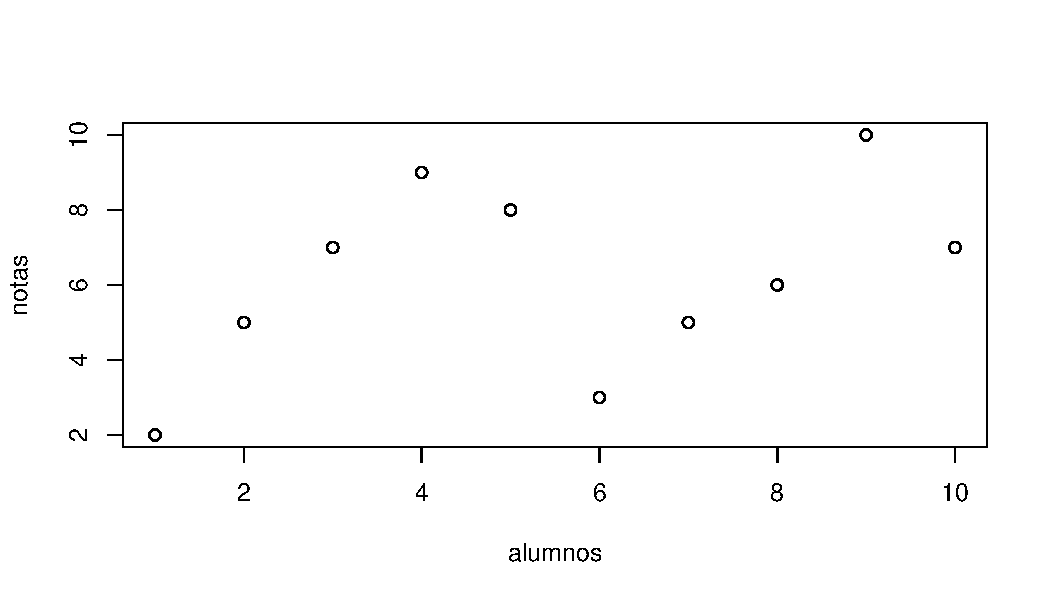
\includegraphics[width=0.8\linewidth]{R_base_files/figure-beamer/unnamed-chunk-35-1} \end{center}
\end{frame}

\begin{frame}[fragile]{Parámetros de la función plot()}
\phantomsection\label{paruxe1metros-de-la-funciuxf3n-plot}
\begin{itemize}
\tightlist
\item
  \texttt{log}: para indicar que queremos el gráfico en escala
  logarítmica
\item
  \texttt{main("título")}: para poner título al gráfico. Si en vez de un
  texto queráis poner una expresión matemática, tenéis que utilizar la
  función \texttt{expression()}
\item
  \texttt{xlab("etiqueta")}: para poner etiqueta al eje \(X\)
\item
  \texttt{ylab("etiqueta")}: para poner etiqueta al eje \(Y\)
\item
  \texttt{pch=n}: para elegir el símbolo de los puntos.
  \(n=0,1,...,25\). El valor por defecto es \texttt{pch\ =\ 1}
\item
  \texttt{cex}: para elegir el tamaño de los símbolos
\item
  \texttt{col="color\ en\ inglés"}: para elegir el color de los
  símbolos.
  \href{http://www.stat.columbia.edu/~tzheng/files/Rcolor.pdf}{Gama de
  colores}.
\end{itemize}
\end{frame}

\begin{frame}{Parámetro pch - Tipos de símbolos}
\phantomsection\label{paruxe1metro-pch---tipos-de-suxedmbolos}
\begin{center}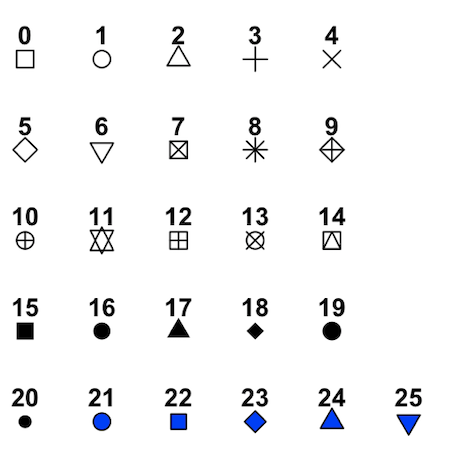
\includegraphics[width=0.6\linewidth]{Imgs/pch} \end{center}
\end{frame}

\begin{frame}[fragile]{Escala logarítmica}
\phantomsection\label{escala-logaruxedtmica}
\begin{Shaded}
\begin{Highlighting}[]
\FunctionTok{par}\NormalTok{(}\AttributeTok{mfrow =} \FunctionTok{c}\NormalTok{(}\DecValTok{1}\NormalTok{,}\DecValTok{2}\NormalTok{))}
\NormalTok{plot }\OtherTok{=} \FunctionTok{plot}\NormalTok{(}\FunctionTok{exp}\NormalTok{(}\DecValTok{1}\SpecialCharTok{:}\DecValTok{20}\NormalTok{), }\AttributeTok{xlab =} \StringTok{"Indice"}\NormalTok{,}
            \AttributeTok{ylab =} \FunctionTok{expression}\NormalTok{(e}\SpecialCharTok{\^{}}\NormalTok{\{}\DecValTok{1}\SpecialCharTok{:}\DecValTok{20}\NormalTok{\}), }
            \AttributeTok{main =} \StringTok{"Escala lineal"}\NormalTok{)}
\NormalTok{plotLog }\OtherTok{=} \FunctionTok{plot}\NormalTok{(}\FunctionTok{exp}\NormalTok{(}\DecValTok{1}\SpecialCharTok{:}\DecValTok{20}\NormalTok{), }\AttributeTok{log =} \StringTok{"y"}\NormalTok{, }\AttributeTok{xlab =} \StringTok{"Indice"}\NormalTok{, }
               \AttributeTok{ylab =} \FunctionTok{expression}\NormalTok{(e}\SpecialCharTok{\^{}}\NormalTok{\{}\DecValTok{1}\SpecialCharTok{:}\DecValTok{20}\NormalTok{\}), }
               \AttributeTok{main =} \StringTok{"Escala logaritmica en el eje y"}\NormalTok{)}
\end{Highlighting}
\end{Shaded}

\begin{center}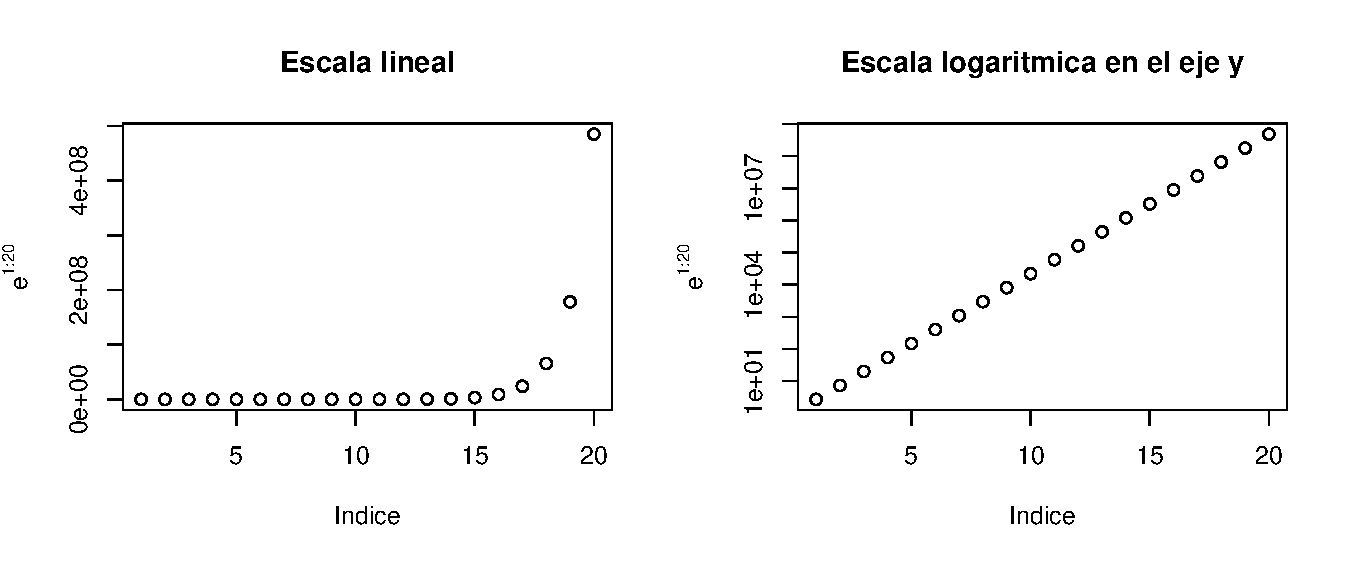
\includegraphics[width=0.7\linewidth]{R_base_files/figure-beamer/unnamed-chunk-36-1} \end{center}

\begin{Shaded}
\begin{Highlighting}[]
\FunctionTok{par}\NormalTok{(}\AttributeTok{mfrow =} \FunctionTok{c}\NormalTok{(}\DecValTok{1}\NormalTok{,}\DecValTok{1}\NormalTok{))}
\end{Highlighting}
\end{Shaded}
\end{frame}

\begin{frame}[fragile]{Parámetros de la función plot()}
\phantomsection\label{paruxe1metros-de-la-funciuxf3n-plot-1}
\begin{itemize}
\tightlist
\item
  \texttt{type}: para elegir el tipo de gráfico que queremos:

  \begin{itemize}
  \tightlist
  \item
    \texttt{p}: puntos (valor por defecto)
  \item
    \texttt{l}: líneas rectas que unen los puntos (dichos puntos no
    tienen símbolo)
  \item
    \texttt{b}: líneas rectas que unen los puntos (dichos puntos tienen
    símbolo). Las líneas no traspasan los puntos
  \item
    \texttt{o}: como el anterior pero en este caso las líneas sí que
    traspasan los puntos
  \item
    \texttt{h}: histograma de líneas
  \item
    \texttt{s}: histograma de escalones
  \item
    \texttt{n}: para no dibujar los puntos
  \end{itemize}
\end{itemize}
\end{frame}

\begin{frame}[fragile]{Tipos de gráfico}
\phantomsection\label{tipos-de-gruxe1fico}
\begin{Shaded}
\begin{Highlighting}[]
\FunctionTok{par}\NormalTok{(}\AttributeTok{mfrow =} \FunctionTok{c}\NormalTok{(}\DecValTok{3}\NormalTok{,}\DecValTok{2}\NormalTok{))}
\NormalTok{x }\OtherTok{=} \FunctionTok{c}\NormalTok{(}\DecValTok{50}\SpecialCharTok{:}\DecValTok{59}\NormalTok{)}
\NormalTok{y }\OtherTok{=} \FunctionTok{c}\NormalTok{(}\DecValTok{2}\NormalTok{,}\DecValTok{9}\NormalTok{,}\DecValTok{25}\NormalTok{,}\DecValTok{3}\NormalTok{,}\DecValTok{100}\NormalTok{,}\DecValTok{77}\NormalTok{,}\DecValTok{62}\NormalTok{,}\DecValTok{54}\NormalTok{,}\DecValTok{19}\NormalTok{,}\DecValTok{40}\NormalTok{)}
\FunctionTok{plot}\NormalTok{(x,y, }\AttributeTok{pch =} \DecValTok{23}\NormalTok{, }\AttributeTok{cex =} \DecValTok{2}\NormalTok{, }\AttributeTok{col =} \StringTok{"blue"}\NormalTok{, }\AttributeTok{type =} \StringTok{"p"}\NormalTok{)}
\FunctionTok{plot}\NormalTok{(x,y, }\AttributeTok{pch =} \DecValTok{23}\NormalTok{, }\AttributeTok{cex =} \DecValTok{2}\NormalTok{, }\AttributeTok{col =} \StringTok{"blueviolet"}\NormalTok{, }\AttributeTok{type =} \StringTok{"l"}\NormalTok{)}
\FunctionTok{plot}\NormalTok{(x,y, }\AttributeTok{pch =} \DecValTok{23}\NormalTok{, }\AttributeTok{cex =} \DecValTok{2}\NormalTok{, }\AttributeTok{col =} \StringTok{"gold"}\NormalTok{, }\AttributeTok{type =} \StringTok{"b"}\NormalTok{)}
\FunctionTok{plot}\NormalTok{(x,y, }\AttributeTok{pch =} \DecValTok{23}\NormalTok{, }\AttributeTok{cex =} \DecValTok{2}\NormalTok{, }\AttributeTok{col =} \StringTok{"deeppink"}\NormalTok{, }\AttributeTok{type =} \StringTok{"o"}\NormalTok{)}
\FunctionTok{plot}\NormalTok{(x,y, }\AttributeTok{pch =} \DecValTok{23}\NormalTok{, }\AttributeTok{cex =} \DecValTok{2}\NormalTok{, }\AttributeTok{col =} \StringTok{"springgreen"}\NormalTok{,}
     \AttributeTok{type =} \StringTok{"h"}\NormalTok{)}
\FunctionTok{plot}\NormalTok{(x,y, }\AttributeTok{pch =} \DecValTok{23}\NormalTok{, }\AttributeTok{cex =} \DecValTok{2}\NormalTok{, }\AttributeTok{col =} \StringTok{"firebrick1"}\NormalTok{,}
     \AttributeTok{type =} \StringTok{"s"}\NormalTok{)}
\FunctionTok{par}\NormalTok{(}\AttributeTok{mfrow =} \FunctionTok{c}\NormalTok{(}\DecValTok{1}\NormalTok{,}\DecValTok{1}\NormalTok{))}
\end{Highlighting}
\end{Shaded}
\end{frame}

\begin{frame}{Tipos de gráfico}
\phantomsection\label{tipos-de-gruxe1fico-1}
\begin{center}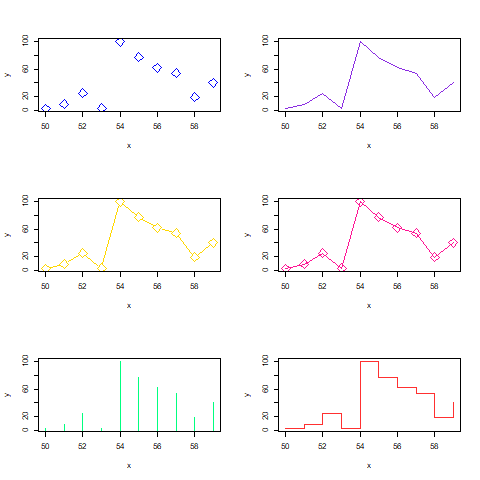
\includegraphics[width=0.7\linewidth]{Imgs/tipo_grafico_1} \end{center}
\end{frame}

\begin{frame}[fragile]{Parámetros de la función plot()}
\phantomsection\label{paruxe1metros-de-la-funciuxf3n-plot-2}
\begin{itemize}
\tightlist
\item
  \texttt{lty}: para especificar el tipo de línea

  \begin{itemize}
  \tightlist
  \item
    ``solid'' : \(1\): línea continua (valor por defecto)
  \item
    ``dashed'' : \(2\): línea discontinua
  \item
    ``dotted'' : \(3\): línea de puntos
  \item
    ``dotdashed'' : \(4\): línea que alterna puntos y rayas
  \end{itemize}
\item
  \texttt{lwd}: para especificar el grosor de las líneas
\item
  \texttt{xlim}: para modificar el rango del eje \(X\)
\item
  \texttt{ylim}: para modificar el rango del eje \(Y\)
\item
  \texttt{xaxp}: para modificar posiciones de las marcas en el eje \(X\)
\item
  \texttt{yaxp}: para modificar posiciones de las marcas en el eje \(Y\)
\end{itemize}
\end{frame}

\begin{frame}[fragile]{Parámetros de la función plot()}
\phantomsection\label{paruxe1metros-de-la-funciuxf3n-plot-3}
\begin{Shaded}
\begin{Highlighting}[]
\NormalTok{x }\OtherTok{=}\NormalTok{ (}\DecValTok{2}\SpecialCharTok{*}\NormalTok{(}\DecValTok{1}\SpecialCharTok{:}\DecValTok{20}\NormalTok{))}
\NormalTok{y }\OtherTok{=}\NormalTok{ (}\SpecialCharTok{{-}}\DecValTok{1}\NormalTok{)}\SpecialCharTok{\^{}}\NormalTok{(}\DecValTok{1}\SpecialCharTok{:}\DecValTok{20}\NormalTok{)}\SpecialCharTok{*}\DecValTok{5}\SpecialCharTok{*}\NormalTok{(}\DecValTok{1}\SpecialCharTok{:}\DecValTok{20}\NormalTok{)}
\FunctionTok{plot}\NormalTok{(x,y, }\AttributeTok{main =} \StringTok{"Ejemplo de grafico"}\NormalTok{, }\AttributeTok{pch =} \DecValTok{8}\NormalTok{, }\AttributeTok{cex =} \DecValTok{1}\NormalTok{,}
     \AttributeTok{type =} \StringTok{"b"}\NormalTok{, }\AttributeTok{lty =} \DecValTok{4}\NormalTok{, }\AttributeTok{lwd =} \DecValTok{4}\NormalTok{, }
     \AttributeTok{xaxp =} \FunctionTok{c}\NormalTok{(}\DecValTok{0}\NormalTok{,}\DecValTok{40}\NormalTok{,}\DecValTok{2}\NormalTok{), }\AttributeTok{yaxp =} \FunctionTok{c}\NormalTok{(}\SpecialCharTok{{-}}\DecValTok{100}\NormalTok{,}\DecValTok{100}\NormalTok{,}\DecValTok{8}\NormalTok{))}
\end{Highlighting}
\end{Shaded}

\begin{center}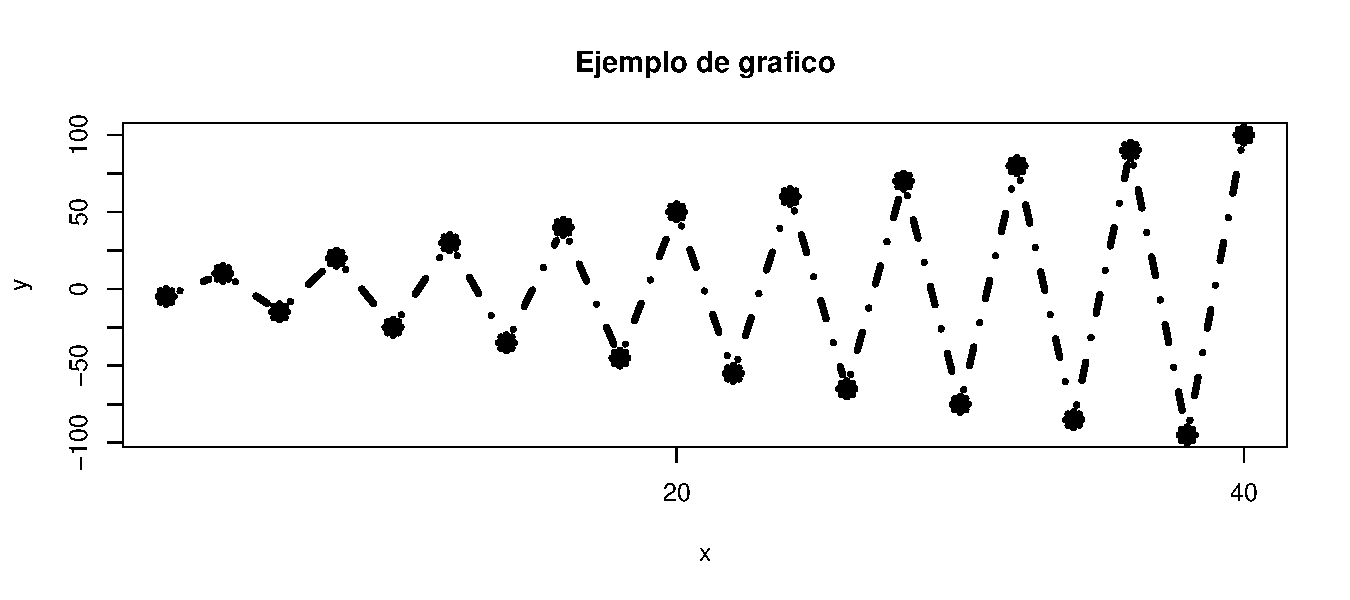
\includegraphics[width=0.8\linewidth]{R_base_files/figure-beamer/unnamed-chunk-38-1} \end{center}
\end{frame}

\begin{frame}[fragile]{Añadir elementos al gráfico}
\phantomsection\label{auxf1adir-elementos-al-gruxe1fico}
\begin{itemize}
\tightlist
\item
  \texttt{points(x,y)}: añade un punto de coordenadas \((x, y)\) a un
  gráfico ya existente
\item
  \texttt{abline}: para añadir una recta a un gráfico ya existente

  \begin{itemize}
  \tightlist
  \item
    \texttt{abline(a,b)}: añade la recta \(y=ax+b\)
  \item
    \texttt{abline(v\ =\ x0)}: añade la recta vertical \(x=x_0\). \(v\)
    puede estar asignado a un vector
  \item
    \texttt{abline(h\ =\ y0)}: añade la recta horizontal \(y=y_0\).
    \(h\) puede estar asignado a un vector
  \end{itemize}
\end{itemize}
\end{frame}

\begin{frame}[fragile]{Añadiendo punto y recta}
\phantomsection\label{auxf1adiendo-punto-y-recta}
\begin{Shaded}
\begin{Highlighting}[]
\NormalTok{x }\OtherTok{=}\NormalTok{ (}\DecValTok{2}\SpecialCharTok{*}\NormalTok{(}\DecValTok{1}\SpecialCharTok{:}\DecValTok{20}\NormalTok{))}
\NormalTok{y }\OtherTok{=}\NormalTok{ (}\SpecialCharTok{{-}}\DecValTok{1}\NormalTok{)}\SpecialCharTok{\^{}}\NormalTok{(}\DecValTok{1}\SpecialCharTok{:}\DecValTok{20}\NormalTok{)}\SpecialCharTok{*}\DecValTok{5}\SpecialCharTok{*}\NormalTok{(}\DecValTok{1}\SpecialCharTok{:}\DecValTok{20}\NormalTok{)}
\FunctionTok{plot}\NormalTok{(x,y, }\AttributeTok{main =} \StringTok{"Poniendo un punto y una recta"}\NormalTok{, }\AttributeTok{pch =} \DecValTok{8}\NormalTok{,}
     \AttributeTok{cex =} \DecValTok{1}\NormalTok{, }\AttributeTok{type =} \StringTok{"b"}\NormalTok{, }\AttributeTok{lty =} \DecValTok{4}\NormalTok{, }
     \AttributeTok{lwd =} \DecValTok{4}\NormalTok{, }\AttributeTok{xaxp =} \FunctionTok{c}\NormalTok{(}\DecValTok{0}\NormalTok{,}\DecValTok{40}\NormalTok{,}\DecValTok{2}\NormalTok{), }\AttributeTok{yaxp =} \FunctionTok{c}\NormalTok{(}\SpecialCharTok{{-}}\DecValTok{100}\NormalTok{,}\DecValTok{100}\NormalTok{,}\DecValTok{8}\NormalTok{))}
\FunctionTok{points}\NormalTok{(}\DecValTok{20}\NormalTok{,}\DecValTok{0}\NormalTok{, }\AttributeTok{col =} \StringTok{"red"}\NormalTok{, }\AttributeTok{cex =} \DecValTok{4}\NormalTok{, }\AttributeTok{pch =} \DecValTok{16}\NormalTok{)}
\FunctionTok{abline}\NormalTok{ (}\AttributeTok{h =} \DecValTok{0}\NormalTok{, }\AttributeTok{lty =} \DecValTok{2}\NormalTok{, }\AttributeTok{col =} \StringTok{"dodgerblue"}\NormalTok{)}
\end{Highlighting}
\end{Shaded}
\end{frame}

\begin{frame}{Añadiendo punto y recta}
\phantomsection\label{auxf1adiendo-punto-y-recta-1}
\begin{center}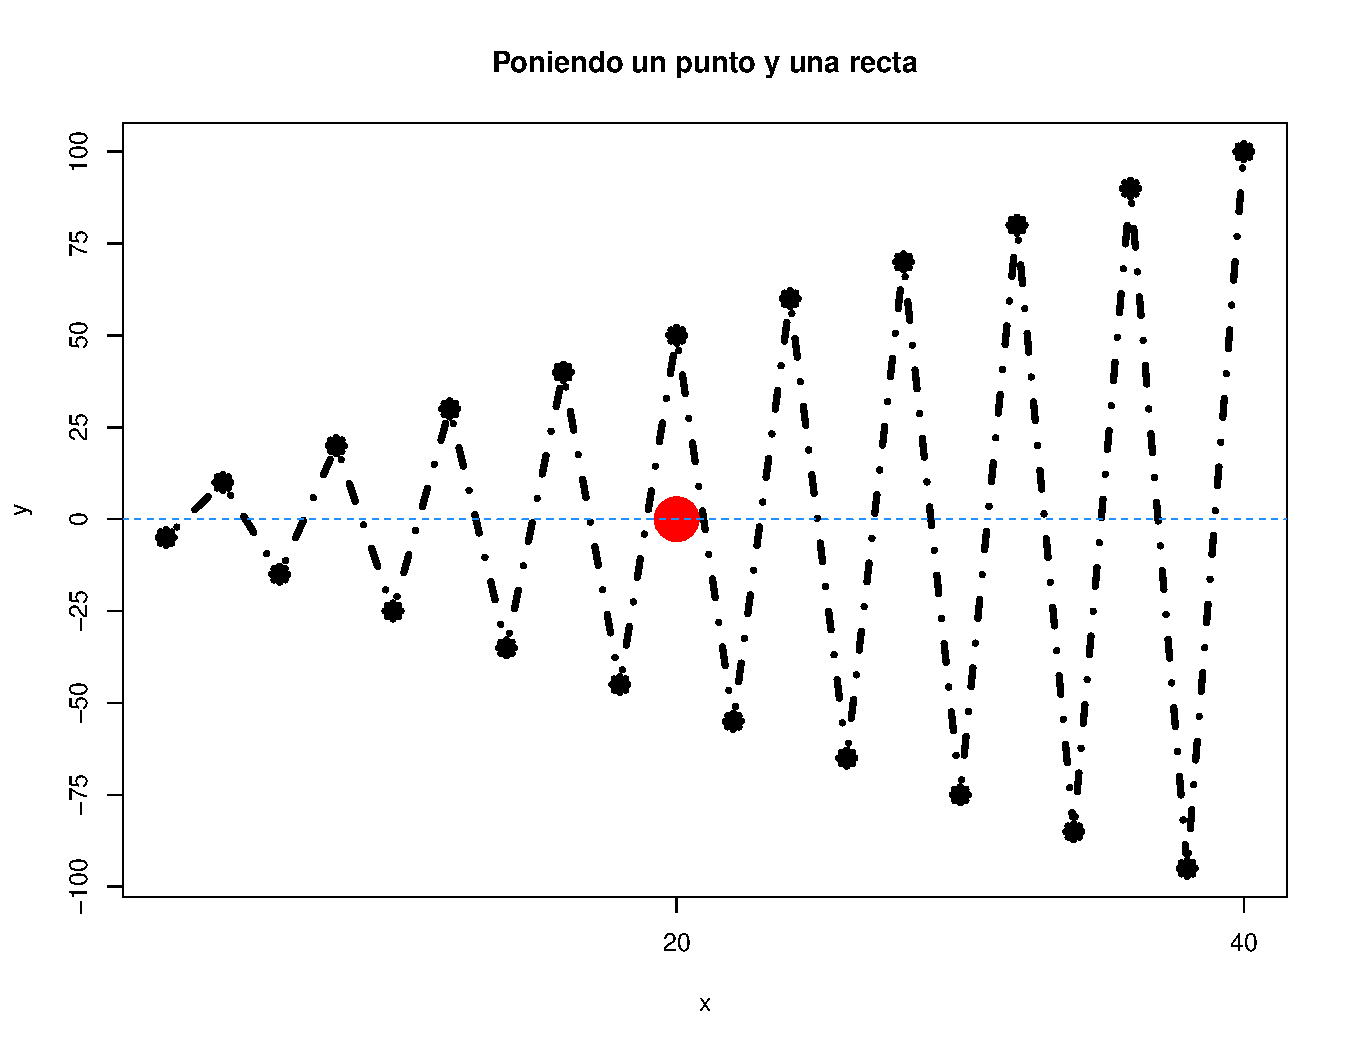
\includegraphics[width=0.8\linewidth]{R_base_files/figure-beamer/unnamed-chunk-40-1} \end{center}
\end{frame}

\begin{frame}[fragile]{Añadir elementos al gráfico}
\phantomsection\label{auxf1adir-elementos-al-gruxe1fico-1}
\begin{itemize}
\tightlist
\item
  \texttt{text(x,y,labels\ =\ "....")}: añade en el punto de coordenadas
  \((x,y)\) el texto especificado como argumento de labels

  \begin{itemize}
  \tightlist
  \item
    \texttt{pos}: permite indicar la posición del texto alrededor de las
    coordenadas \((x,y)\). Admite los siguientes valores:

    \begin{itemize}
    \tightlist
    \item
      1: abajo
    \item
      2: izquierda
    \item
      3: arriba
    \item
      4: derecha
    \item
      5: sin especificar: el texto se sitúa centrado en el punto
      \((x,y)\)
    \end{itemize}
  \end{itemize}
\end{itemize}
\end{frame}

\begin{frame}[fragile]{Añadiendo etiquetas}
\phantomsection\label{auxf1adiendo-etiquetas}
\begin{Shaded}
\begin{Highlighting}[]
\NormalTok{alumnos }\OtherTok{=} \FunctionTok{c}\NormalTok{(}\DecValTok{1}\SpecialCharTok{:}\DecValTok{10}\NormalTok{)}
\NormalTok{notas }\OtherTok{=} \FunctionTok{c}\NormalTok{(}\DecValTok{2}\NormalTok{,}\DecValTok{5}\NormalTok{,}\DecValTok{7}\NormalTok{,}\DecValTok{9}\NormalTok{,}\DecValTok{8}\NormalTok{,}\DecValTok{3}\NormalTok{,}\DecValTok{5}\NormalTok{,}\DecValTok{6}\NormalTok{,}\DecValTok{10}\NormalTok{,}\DecValTok{7}\NormalTok{)}
\FunctionTok{plot}\NormalTok{(alumnos,notas, }\AttributeTok{main =} \StringTok{"Grafico con texto"}\NormalTok{)}
\FunctionTok{text}\NormalTok{(alumnos,notas, }
     \AttributeTok{labels =} \FunctionTok{c}\NormalTok{(}\StringTok{"S"}\NormalTok{,}\StringTok{"A"}\NormalTok{,}\StringTok{"N"}\NormalTok{,}\StringTok{"E"}\NormalTok{,}\StringTok{"N"}\NormalTok{,}\StringTok{"S"}\NormalTok{,}\StringTok{"A"}\NormalTok{,}\StringTok{"A"}\NormalTok{,}\StringTok{"E"}\NormalTok{,}\StringTok{"N"}\NormalTok{), }
     \AttributeTok{pos =} \FunctionTok{c}\NormalTok{(}\FunctionTok{rep}\NormalTok{(}\DecValTok{3}\NormalTok{,}\AttributeTok{times =} \DecValTok{8}\NormalTok{),}\DecValTok{1}\NormalTok{,}\DecValTok{3}\NormalTok{))}
\end{Highlighting}
\end{Shaded}

\begin{center}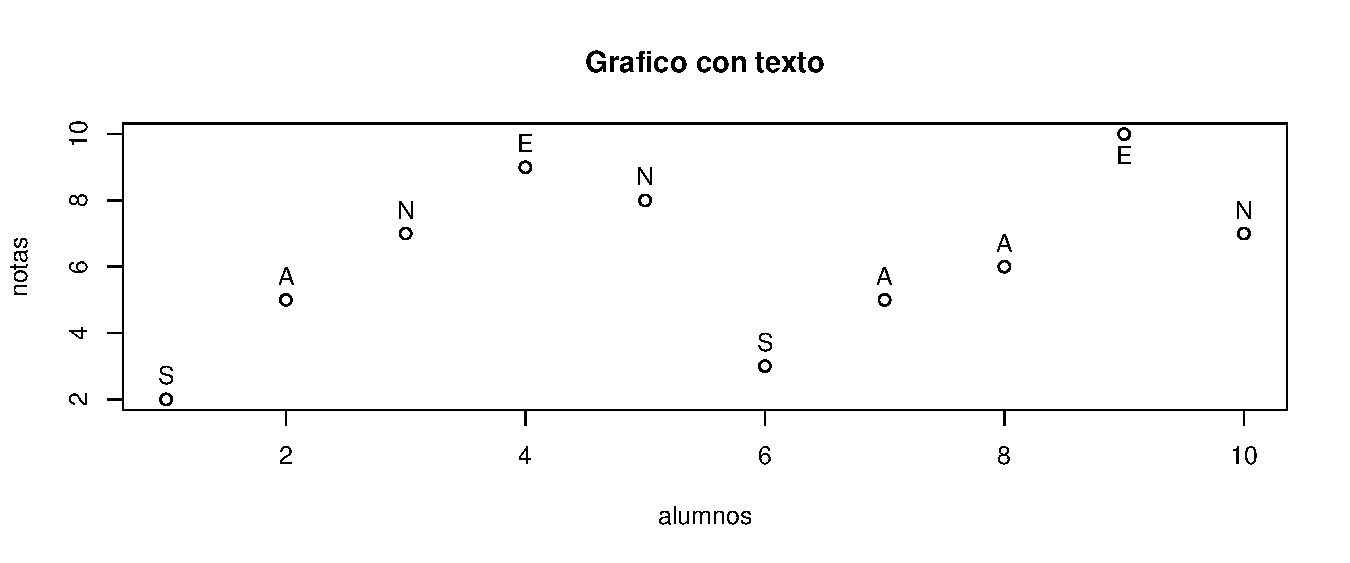
\includegraphics[width=0.8\linewidth]{R_base_files/figure-beamer/unnamed-chunk-41-1} \end{center}
\end{frame}

\begin{frame}[fragile]{Añadir elementos al gráfico}
\phantomsection\label{auxf1adir-elementos-al-gruxe1fico-2}
\begin{itemize}
\tightlist
\item
  \texttt{lines(x,\ y)}:añade a un gráfico existente una línea poligonal
  que une los puntos \((x_i, y_i)\) sucesivos. \(x,y\) son vectores
  numéricos
\item
  \texttt{curve(curva)}: permite añadir la gráfica de una curva a un
  gráfico existente

  \begin{itemize}
  \tightlist
  \item
    \texttt{add=TRUE}: si no, la curva no se añade
  \item
    La curva se puede especificar mediante una expresión algebraica con
    variable \(x\), o mediante su nombre si la hemos definido antes
  \end{itemize}
\end{itemize}
\end{frame}

\begin{frame}[fragile]{Añadiendo líneas y curvas}
\phantomsection\label{auxf1adiendo-luxedneas-y-curvas}
\begin{Shaded}
\begin{Highlighting}[]
\NormalTok{x }\OtherTok{=} \FunctionTok{c}\NormalTok{(}\DecValTok{5}\SpecialCharTok{*}\NormalTok{(}\DecValTok{1}\SpecialCharTok{:}\DecValTok{20}\NormalTok{))}
\FunctionTok{plot}\NormalTok{(x,}\FunctionTok{c}\NormalTok{(}\FunctionTok{exp}\NormalTok{(}\SpecialCharTok{{-}}\NormalTok{x)}\SpecialCharTok{+}\NormalTok{(}\SpecialCharTok{{-}}\DecValTok{1}\NormalTok{)}\SpecialCharTok{\^{}}\NormalTok{x}\SpecialCharTok{*}\NormalTok{x}\SpecialCharTok{/}\DecValTok{2}\SpecialCharTok{*}\FunctionTok{sin}\NormalTok{(x)}\SpecialCharTok{\^{}}\DecValTok{2}\NormalTok{))}
\FunctionTok{lines}\NormalTok{(}\FunctionTok{c}\NormalTok{(}\DecValTok{20}\NormalTok{,}\DecValTok{10}\NormalTok{,}\DecValTok{40}\NormalTok{,}\DecValTok{80}\NormalTok{,}\DecValTok{60}\NormalTok{,}\DecValTok{60}\NormalTok{,}\DecValTok{20}\NormalTok{),}\FunctionTok{c}\NormalTok{(}\DecValTok{20}\NormalTok{,}\DecValTok{0}\NormalTok{,}\SpecialCharTok{{-}}\DecValTok{20}\NormalTok{,}\SpecialCharTok{{-}}\DecValTok{20}\NormalTok{,}\DecValTok{40}\NormalTok{,}\DecValTok{0}\NormalTok{,}\DecValTok{20}\NormalTok{), }
      \AttributeTok{lwd =} \DecValTok{2}\NormalTok{, }\AttributeTok{col =} \StringTok{"darkslategray1"}\NormalTok{)}
\FunctionTok{curve}\NormalTok{(}\DecValTok{20}\SpecialCharTok{*}\FunctionTok{sin}\NormalTok{(x), }\AttributeTok{add =} \ConstantTok{TRUE}\NormalTok{, }\AttributeTok{col =} \StringTok{"green"}\NormalTok{)}
\end{Highlighting}
\end{Shaded}

\begin{center}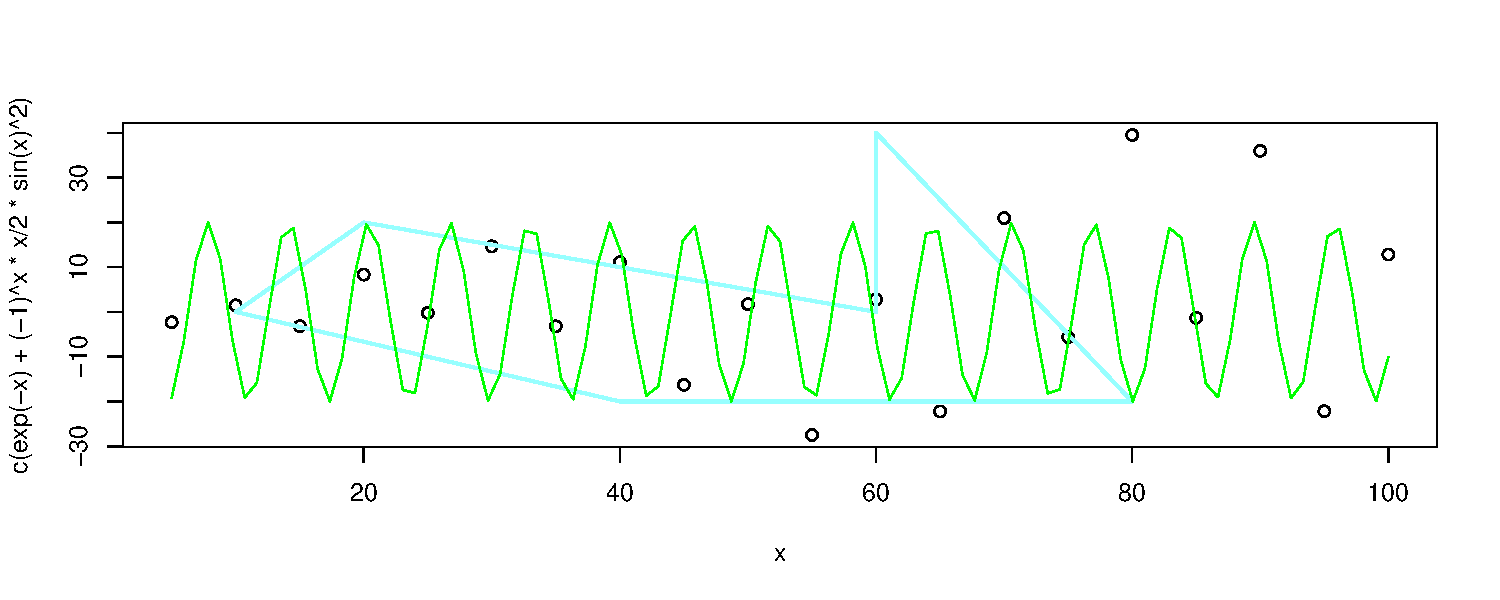
\includegraphics[width=0.8\linewidth]{R_base_files/figure-beamer/unnamed-chunk-42-1} \end{center}
\end{frame}

\begin{frame}[fragile]{Añadir elementos al gráfico}
\phantomsection\label{auxf1adir-elementos-al-gruxe1fico-3}
\begin{itemize}
\tightlist
\item
  \texttt{legend(posición,\ legend\ =\ ...)}: para añadir una leyenda

  \begin{itemize}
  \tightlist
  \item
    La posición indica donde queremos situar la leyenda. Puede ser o
    bien las coordenadas de la esquina superior izquierda de nuestra
    leyenda, o bien una de las palabras siguientes:

    \begin{itemize}
    \tightlist
    \item
      ``bottom'' / ``bottomright'' / ``bottomleft''
    \item
      ``top'' / ``topright'' / ``topleft''
    \item
      ``center'' / ``right'' / ``left''
    \end{itemize}
  \item
    \texttt{legend}: contiene el vector de nombres entre comillas con
    los que queremos identificar a las curvas en la leyenda
  \end{itemize}
\end{itemize}
\end{frame}

\begin{frame}[fragile]{Añadiendo leyenda}
\phantomsection\label{auxf1adiendo-leyenda}
\begin{Shaded}
\begin{Highlighting}[]
\NormalTok{x }\OtherTok{=} \FunctionTok{seq}\NormalTok{(}\DecValTok{0}\NormalTok{,}\DecValTok{2}\SpecialCharTok{*}\NormalTok{pi,}\FloatTok{0.1}\NormalTok{)}
\FunctionTok{plot}\NormalTok{(x,}\FunctionTok{sin}\NormalTok{(x),}\AttributeTok{type=}\StringTok{"l"}\NormalTok{,}\AttributeTok{col=}\StringTok{"blue"}\NormalTok{,}\AttributeTok{lwd=}\DecValTok{3}\NormalTok{, }\AttributeTok{xlab=}\StringTok{""}\NormalTok{, }\AttributeTok{ylab=}\StringTok{""}\NormalTok{)}
\FunctionTok{lines}\NormalTok{(x,}\FunctionTok{cos}\NormalTok{(x),}\AttributeTok{col=}\StringTok{"green"}\NormalTok{,}\AttributeTok{lwd=}\DecValTok{3}\NormalTok{)}
\FunctionTok{lines}\NormalTok{(x, }\FunctionTok{tan}\NormalTok{(x), }\AttributeTok{col=}\StringTok{"purple"}\NormalTok{,}\AttributeTok{lwd=}\DecValTok{3}\NormalTok{)}
\FunctionTok{legend}\NormalTok{(}\StringTok{"bottomleft"}\NormalTok{,}\AttributeTok{col=}\FunctionTok{c}\NormalTok{(}\StringTok{"blue"}\NormalTok{,}\StringTok{"green"}\NormalTok{,}\StringTok{"purple"}\NormalTok{), }
       \AttributeTok{legend=}\FunctionTok{c}\NormalTok{(}\StringTok{"Seno"}\NormalTok{,}\StringTok{"Coseno"}\NormalTok{, }\StringTok{"Tangente"}\NormalTok{), }
       \AttributeTok{lwd=}\DecValTok{3}\NormalTok{, }\AttributeTok{bty=}\StringTok{"l"}\NormalTok{)}
\end{Highlighting}
\end{Shaded}
\end{frame}

\begin{frame}{Añadiendo leyenda}
\phantomsection\label{auxf1adiendo-leyenda-1}
\begin{center}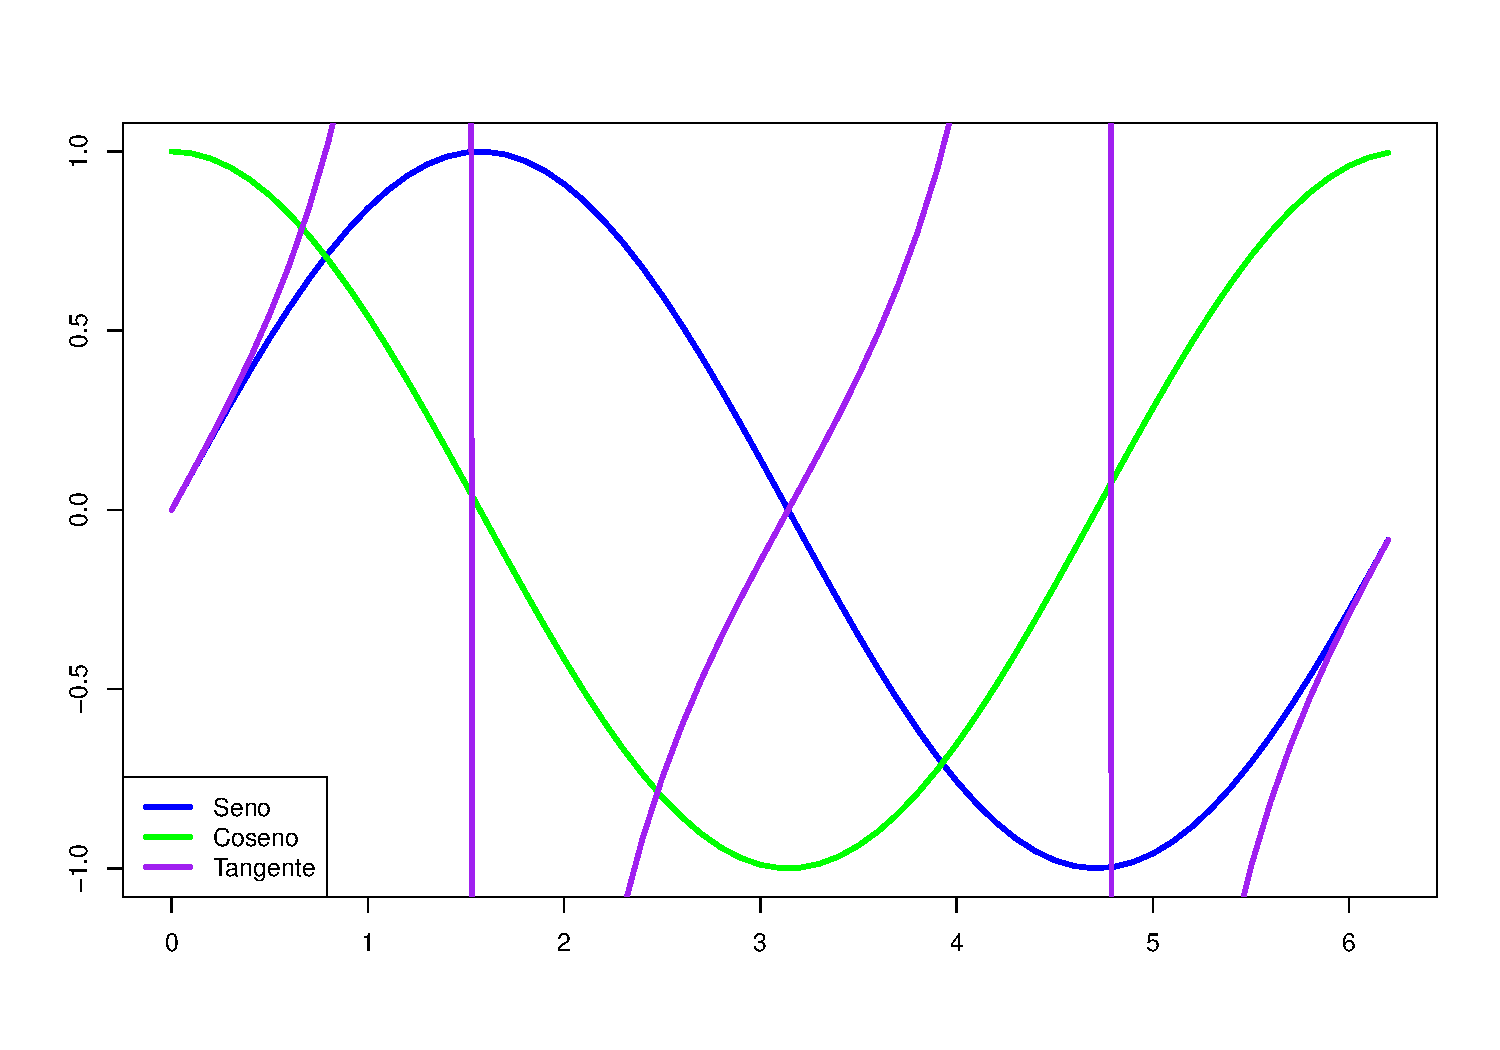
\includegraphics[width=0.8\linewidth]{R_base_files/figure-beamer/unnamed-chunk-44-1} \end{center}
\end{frame}

\begin{frame}[fragile]{Añadir elementos al gráfico}
\phantomsection\label{auxf1adir-elementos-al-gruxe1fico-4}
\begin{itemize}
\tightlist
\item
  \texttt{segments}: para añadir segmentos a un gráfico existente
\item
  \texttt{arrows}: para añadir flechas a un gráfico existente
\item
  \texttt{symbols}: para añadir símbolos a un gráfico existente
\item
  \texttt{polygon}: para añadir polígonos cerrados especificando sus
  vértices a un gráfico existente
\end{itemize}
\end{frame}

\begin{frame}[fragile]{Añadiendo elementos}
\phantomsection\label{auxf1adiendo-elementos}
\begin{Shaded}
\begin{Highlighting}[]
\NormalTok{x }\OtherTok{=} \FunctionTok{c}\NormalTok{(}\DecValTok{5}\SpecialCharTok{*}\NormalTok{(}\DecValTok{1}\SpecialCharTok{:}\DecValTok{10}\NormalTok{))}
\FunctionTok{plot}\NormalTok{(x,}\FunctionTok{c}\NormalTok{(}\FunctionTok{exp}\NormalTok{(}\SpecialCharTok{{-}}\NormalTok{x)}\SpecialCharTok{+}\NormalTok{(}\SpecialCharTok{{-}}\DecValTok{1}\NormalTok{)}\SpecialCharTok{\^{}}\NormalTok{x}\SpecialCharTok{*}\NormalTok{x}\SpecialCharTok{/}\DecValTok{2}\SpecialCharTok{*}\FunctionTok{sin}\NormalTok{(x)}\SpecialCharTok{\^{}}\DecValTok{2}\NormalTok{), }\AttributeTok{xlab =} \StringTok{""}\NormalTok{, }\AttributeTok{ylab =} \StringTok{""}\NormalTok{, }
     \AttributeTok{main =} \StringTok{"Grafico con varios elementos"}\NormalTok{)}
\FunctionTok{segments}\NormalTok{(}\DecValTok{10}\NormalTok{,}\DecValTok{0}\NormalTok{,}\DecValTok{40}\NormalTok{,}\DecValTok{0}\NormalTok{, }\AttributeTok{col =} \StringTok{"red"}\NormalTok{, }\AttributeTok{lwd =} \DecValTok{4}\NormalTok{)}
\FunctionTok{arrows}\NormalTok{(}\DecValTok{10}\NormalTok{,}\DecValTok{0}\NormalTok{,}\DecValTok{40}\NormalTok{,}\SpecialCharTok{{-}}\DecValTok{10}\NormalTok{, }\AttributeTok{col =} \StringTok{" blue"}\NormalTok{, }\AttributeTok{length =} \FloatTok{0.5}\NormalTok{,}
       \AttributeTok{angle =} \DecValTok{5}\NormalTok{, }\AttributeTok{code =} \DecValTok{3}\NormalTok{)}
\FunctionTok{symbols}\NormalTok{(}\DecValTok{40}\NormalTok{,}\DecValTok{0}\NormalTok{,}\AttributeTok{stars =} \FunctionTok{cbind}\NormalTok{(}\DecValTok{1}\NormalTok{,.}\DecValTok{5}\NormalTok{,}\DecValTok{1}\NormalTok{,.}\DecValTok{5}\NormalTok{,}\DecValTok{1}\NormalTok{,.}\DecValTok{5}\NormalTok{,}\DecValTok{1}\NormalTok{,.}\DecValTok{5}\NormalTok{,}\DecValTok{1}\NormalTok{,.}\DecValTok{5}\NormalTok{), }
        \AttributeTok{add =} \ConstantTok{TRUE}\NormalTok{, }\AttributeTok{lwd =} \DecValTok{3}\NormalTok{, }\AttributeTok{inches =} \FloatTok{0.5}\NormalTok{)}
\FunctionTok{symbols}\NormalTok{(}\DecValTok{40}\NormalTok{,}\DecValTok{0}\NormalTok{,}\AttributeTok{stars =} \FunctionTok{cbind}\NormalTok{(}\DecValTok{1}\NormalTok{,.}\DecValTok{5}\NormalTok{,}\DecValTok{1}\NormalTok{,.}\DecValTok{5}\NormalTok{,}\DecValTok{1}\NormalTok{,.}\DecValTok{5}\NormalTok{,}\DecValTok{1}\NormalTok{,.}\DecValTok{5}\NormalTok{,}\DecValTok{1}\NormalTok{,.}\DecValTok{5}\NormalTok{),}
        \AttributeTok{add =} \ConstantTok{TRUE}\NormalTok{, }\AttributeTok{lwd =} \DecValTok{3}\NormalTok{)}
\FunctionTok{polygon}\NormalTok{(}\FunctionTok{c}\NormalTok{(}\DecValTok{20}\NormalTok{,}\DecValTok{30}\NormalTok{,}\DecValTok{40}\NormalTok{),}\FunctionTok{c}\NormalTok{(}\DecValTok{10}\NormalTok{,}\SpecialCharTok{{-}}\DecValTok{10}\NormalTok{,}\DecValTok{10}\NormalTok{), }\AttributeTok{col =} \StringTok{"gold"}\NormalTok{,}
        \AttributeTok{density =} \DecValTok{3}\NormalTok{, }\AttributeTok{angle =} \DecValTok{90}\NormalTok{, }\AttributeTok{lty =} \DecValTok{4}\NormalTok{, }
        \AttributeTok{lwd =} \DecValTok{5}\NormalTok{)}
\end{Highlighting}
\end{Shaded}
\end{frame}

\begin{frame}{Añadiendo elementos}
\phantomsection\label{auxf1adiendo-elementos-1}
\begin{center}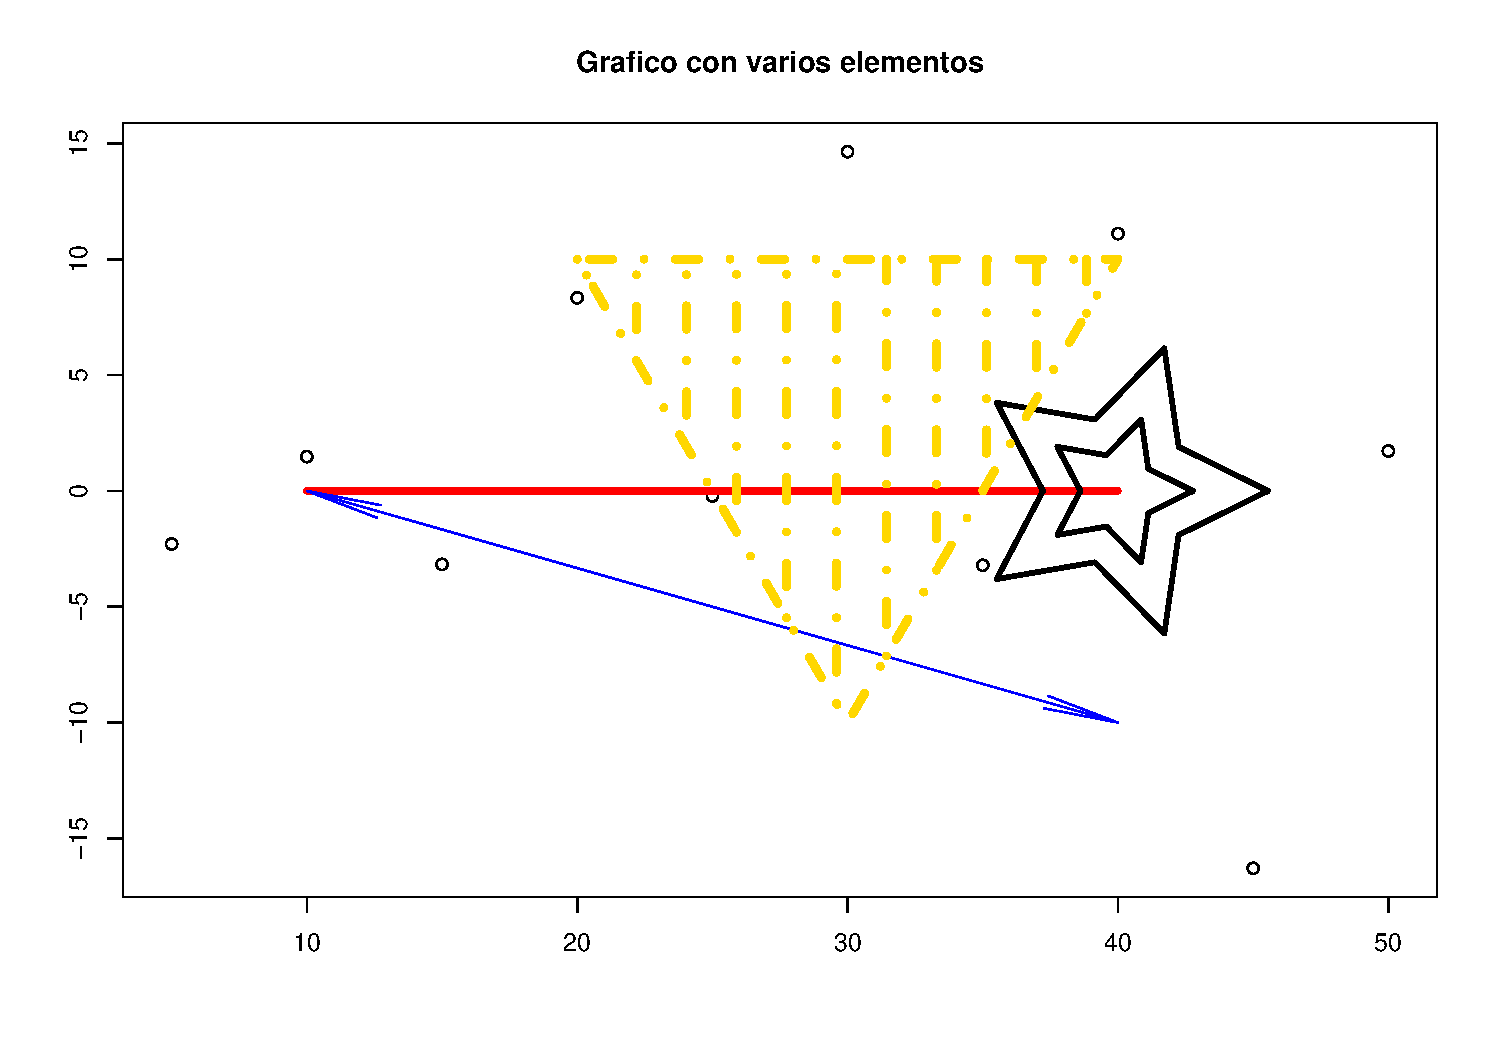
\includegraphics[width=0.8\linewidth]{R_base_files/figure-beamer/unnamed-chunk-46-1} \end{center}
\end{frame}

\section{Hojas de datos: data frames}\label{hojas-de-datos-data-frames}

\begin{frame}[fragile]{Data frames}
\phantomsection\label{data-frames}
\blue{Data frame.} Un data frame es una tabla de doble entrada, formada
por variables en las columnas y observaciones de estas variables en las
filas, de manera que cada fila contiene los valores de las variables
para un mismo caso o un mismo individuo.

\begin{itemize}
\item
  \texttt{data()}: para abrir una ventana con la lista de los objetos de
  datos a los que tenemos acceso en la sesión actual de R (los que lleva
  la instalación básica de R y los que aportan los paquetes que tengamos
  cargados.

  \begin{itemize}
  \tightlist
  \item
    Si entramos \texttt{data(package=.packages(all.available\ =\ TRUE))}
    obtendremos la lista de todos los objetos de datos a los que tenemos
    acceso, incluyendo los de los paquetes que tengamos instalados, pero
    que no estén cargados en la sesión actual.
  \end{itemize}
\end{itemize}
\end{frame}

\begin{frame}[fragile]{Acceder a la información, estructura y atributos
de un data frame}
\phantomsection\label{acceder-a-la-informaciuxf3n-estructura-y-atributos-de-un-data-frame}
\begin{itemize}
\tightlist
\item
  \texttt{head(d.f,n)}: para mostrar las \(n\) primeras filas del data
  frame. Por defecto se muestran las 6 primeras filas
\item
  \texttt{tail(d.f,n)}: para mostrar las \(n\) últimas filas del data
  frame. Por defecto semuestran las 6 últimas
\item
  \texttt{str(d.f)}: para conocer la estructura global de un data frame
\item
  \texttt{names(d.f)}: para producir un vector con los nombres de las
  columnas
\end{itemize}
\end{frame}

\begin{frame}[fragile]{Acceder a la información, estructura y atributos
de un data frame}
\phantomsection\label{acceder-a-la-informaciuxf3n-estructura-y-atributos-de-un-data-frame-1}
\begin{Shaded}
\begin{Highlighting}[]
\FunctionTok{str}\NormalTok{(Orange)}
\end{Highlighting}
\end{Shaded}

\begin{verbatim}
Classes 'nfnGroupedData', 'nfGroupedData', 'groupedData' and 'data.frame':  35 obs. of  3 variables:
 $ Tree         : Ord.factor w/ 5 levels "3"<"1"<"5"<"2"<..: 2 2 2 2 2 2 2 4 4 4 ...
 $ age          : num  118 484 664 1004 1231 ...
 $ circumference: num  30 58 87 115 120 142 145 33 69 111 ...
 - attr(*, "formula")=Class 'formula'  language circumference ~ age | Tree
  .. ..- attr(*, ".Environment")=<environment: R_EmptyEnv> 
 - attr(*, "labels")=List of 2
  ..$ x: chr "Time since December 31, 1968"
  ..$ y: chr "Trunk circumference"
 - attr(*, "units")=List of 2
  ..$ x: chr "(days)"
  ..$ y: chr "(mm)"
\end{verbatim}
\end{frame}

\begin{frame}[fragile]{Acceder a la información, estructura y atributos
de un data frame}
\phantomsection\label{acceder-a-la-informaciuxf3n-estructura-y-atributos-de-un-data-frame-2}
\begin{Shaded}
\begin{Highlighting}[]
\FunctionTok{head}\NormalTok{(Orange,}\DecValTok{4}\NormalTok{)}
\end{Highlighting}
\end{Shaded}

\begin{verbatim}
  Tree  age circumference
1    1  118            30
2    1  484            58
3    1  664            87
4    1 1004           115
\end{verbatim}

\begin{Shaded}
\begin{Highlighting}[]
\FunctionTok{tail}\NormalTok{(Orange,}\DecValTok{4}\NormalTok{)}
\end{Highlighting}
\end{Shaded}

\begin{verbatim}
   Tree  age circumference
32    5 1004           125
33    5 1231           142
34    5 1372           174
35    5 1582           177
\end{verbatim}
\end{frame}

\begin{frame}[fragile]{Acceder a la información, estructura y atributos
de un data frame}
\phantomsection\label{acceder-a-la-informaciuxf3n-estructura-y-atributos-de-un-data-frame-3}
\begin{itemize}
\tightlist
\item
  \texttt{rownames(d.f)}: para producir un vector con los
  identificadores de las filas

  \begin{itemize}
  \tightlist
  \item
    R entiende siempre que estos identificadores son palabras, aunque
    sean números, de ahí que los imprima entre comillas
  \end{itemize}
\item
  \texttt{colnames(d.f)}: para producir un vector con los
  identificadores de las columnas
\item
  \texttt{dimnames(d.f)}: para producir una list formada por dos
  vectores (el de los identificadores de las filas y el de los nombres
  de las columnas)
\item
  \texttt{nrow(d.f)}: para consultar el número de filas de un data frame
\item
  \texttt{ncol(d.f)}: para consultar el número de columnas de un data
  frame
\item
  \texttt{dim(d.f)}: para producir un vector con el número de filas y el
  de columnas
\end{itemize}
\end{frame}

\begin{frame}[fragile]{Acceder a la información, estructura y atributos
de un data frame}
\phantomsection\label{acceder-a-la-informaciuxf3n-estructura-y-atributos-de-un-data-frame-4}
\begin{itemize}
\tightlist
\item
  \texttt{d.f\$nombre\_variable}: para obtener una columna concreta de
  un dataframe

  \begin{itemize}
  \tightlist
  \item
    El resultado será un vector o un factor, según cómo esté definida la
    columna dentro del data frame
  \item
    Las variables de un data frame son internas, no están definidas en
    el entorno global de trabajo de R
  \end{itemize}
\end{itemize}
\end{frame}

\begin{frame}[fragile]{Sub-data frames}
\phantomsection\label{sub-data-frames}
\begin{itemize}
\tightlist
\item
  \texttt{d.f{[}n,m{]}}: para extraer ``trozos'' del data frame por
  filas y columnas (funciona exactamente igual que en matrices) donde
  \(n\) y \(m\) pueden definirse como:

  \begin{itemize}
  \tightlist
  \item
    intervalos
  \item
    condiciones
  \item
    números naturales
  \item
    no poner nada
  \item
    Si sólo queremos definir la subtabla quedándonos con algunas
    variables, basta aplicar el nombre del data frame al vector de
    variables
  \item
    Estas construcciones se pueden usar también para reordenar las filas
    o columnas
  \end{itemize}
\end{itemize}
\end{frame}

\begin{frame}[fragile]{Sub-data frames}
\phantomsection\label{sub-data-frames-1}
\begin{Shaded}
\begin{Highlighting}[]
\NormalTok{dataOrange }\OtherTok{=}\NormalTok{ Orange}
\NormalTok{dataOrange[}\FunctionTok{c}\NormalTok{(}\DecValTok{10}\SpecialCharTok{:}\DecValTok{12}\NormalTok{),]}
\end{Highlighting}
\end{Shaded}

\begin{verbatim}
   Tree  age circumference
10    2  664           111
11    2 1004           156
12    2 1231           172
\end{verbatim}

\begin{Shaded}
\begin{Highlighting}[]
\NormalTok{dataOrange[}\FunctionTok{c}\NormalTok{(}\DecValTok{2}\NormalTok{,}\DecValTok{17}\NormalTok{),}\FunctionTok{c}\NormalTok{(}\DecValTok{1}\NormalTok{,}\DecValTok{3}\NormalTok{)]}
\end{Highlighting}
\end{Shaded}

\begin{verbatim}
   Tree circumference
2     1            58
17    3            75
\end{verbatim}
\end{frame}

\begin{frame}[fragile]{Sub-data frames}
\phantomsection\label{sub-data-frames-2}
\begin{Shaded}
\begin{Highlighting}[]
\NormalTok{dataOrange[}\DecValTok{2}\NormalTok{,}\DecValTok{3}\NormalTok{]}
\end{Highlighting}
\end{Shaded}

\begin{verbatim}
[1] 58
\end{verbatim}

\begin{Shaded}
\begin{Highlighting}[]
\NormalTok{dataOrange[dataOrange}\SpecialCharTok{$}\NormalTok{circumference}\SpecialCharTok{\textless{}=}\DecValTok{50}\NormalTok{,]}
\end{Highlighting}
\end{Shaded}

\begin{verbatim}
   Tree age circumference
1     1 118            30
8     2 118            33
15    3 118            30
22    4 118            32
29    5 118            30
30    5 484            49
\end{verbatim}
\end{frame}

\begin{frame}[fragile]{Leyendo tablas de datos}
\phantomsection\label{leyendo-tablas-de-datos}
\begin{itemize}
\tightlist
\item
  \texttt{read.table()}: para definir un data frame a partir de una
  tabla de datos contenida en un fichero

  \begin{itemize}
  \tightlist
  \item
    Este fichero puede estar guardado en nuestro ordenador o bien
    podemos conocer su url. Sea cual sea el caso, se aplica la función
    al nombre del fichero o a la dirección entre comillas
  \end{itemize}
\end{itemize}

Aquí tenéis una \href{http://aprender.uib.es/}{lista de data frames}
para practicar
\end{frame}

\begin{frame}[fragile]{Parámetros de la función read.table()}
\phantomsection\label{paruxe1metros-de-la-funciuxf3n-read.table}
\begin{itemize}
\tightlist
\item
  \texttt{header\ =\ TRUE}: para indicar si la tabla que importamos
  tiene una primera fila con los nombres de las columnas. El valor por
  defecto es FALSE
\item
  \texttt{col.names\ =\ c(...)}: para especificar el nombre de las
  columnas. No olvidéis que cada nombre debe ir entre comillas
\item
  \texttt{sep}: para especificar las separaciones entre columnas en el
  fichero (si no es un espacio en blanco). Si es así, hay que introducir
  el parámetro pertinente entre comillas
\item
  \texttt{dec}: para especificar el signo que separa la parte entera de
  la decimal (si no es un punto. Si es así, hay que introducir el
  parámetro pertinente entre comillas
\end{itemize}
\end{frame}

\begin{frame}[fragile]{Parámetros de read.table()}
\phantomsection\label{paruxe1metros-de-read.table}
\begin{Shaded}
\begin{Highlighting}[]
\NormalTok{notas }\OtherTok{=} \FunctionTok{read.table}\NormalTok{(}
  \StringTok{"http://aprender.uib.es/Rdir/Controls11{-}12.txt"}\NormalTok{, }
  \AttributeTok{col.names =} \FunctionTok{c}\NormalTok{(}\StringTok{"Nota\_Parcial"}\NormalTok{,}\StringTok{"Nota\_Final"}\NormalTok{,}\StringTok{"Grup"}\NormalTok{),}
  \AttributeTok{sep=}\StringTok{","}\NormalTok{,}\AttributeTok{header=}\ConstantTok{TRUE}\NormalTok{)}
\FunctionTok{head}\NormalTok{(notas,}\DecValTok{8}\NormalTok{)}
\end{Highlighting}
\end{Shaded}

\begin{verbatim}
  Nota_Parcial Nota_Final Grup
1           35         34    1
2           45         30    0
3           64         19    1
4           67         30    0
5           82         31    0
6           50         34    1
7           68         30    0
8           46         23    2
\end{verbatim}
\end{frame}

\begin{frame}[fragile]{Más parámetros de read.table()}
\phantomsection\label{muxe1s-paruxe1metros-de-read.table}
\begin{itemize}
\item
  \texttt{stringsAsFactors}: para prohibir la transformación de las
  columnas de palabras en factores debemos usar
  \texttt{stringsAsFactors=FALSE} (ya que por defecto, R realiza dicha
  transformación)
\item
  Para importar un fichero de una página web segura (cuyo url empiece
  con https), no podemos entrar directamente la dirección en
  \texttt{read.table()}; una solución es instalar y cargar el paquete
  RCurl y entonces usar la instrucción
  \texttt{read.table\ (textConnection(getURL(“url\ ”)),...)}.
\end{itemize}
\end{frame}

\begin{frame}[fragile]{Otros formatos de fichero de datos}
\phantomsection\label{otros-formatos-de-fichero-de-datos}
\begin{itemize}
\tightlist
\item
  \texttt{read.csv()}: para importar ficheros en formato CSV
\item
  \texttt{read.xls()} o \texttt{read.xlsx()}: para importar hojas de
  cálculo tipo Excel u OpenOffice en formato XLS o XLSX,
  respectivamente. Se necesita el paquete xlsx
\item
  \texttt{read.mtb()}: para importar tablas de datos Minitab. Se
  necesita el paquete foreign
\item
  \texttt{read.spss()}: para importar tablas de datos SPSS. Se necesita
  el paquete foreign
\end{itemize}
\end{frame}

\begin{frame}[fragile]{Exportación de datos a ficheros}
\phantomsection\label{exportaciuxf3n-de-datos-a-ficheros}
\begin{itemize}
\tightlist
\item
  \texttt{write.table(df,\ file\ =\ "")}: para exportar un data frame a
  un fichero

  \begin{itemize}
  \tightlist
  \item
    \texttt{file\ =\ ""}: es donde indicaremos el nombre que queremos
    darle al fichero
  \item
    Podemos usar el parámetro \texttt{sep} para indicar el símbolo de
    separación de columnas. Siempre entre comillas
  \item
    También podemos utilizar el parámetro \texttt{dec} para indicar la
    separación entre la parte entera y decimal de los datos
  \end{itemize}
\end{itemize}
\end{frame}

\begin{frame}[fragile]{Exportando datos a ficheros}
\phantomsection\label{exportando-datos-a-ficheros}
\begin{Shaded}
\begin{Highlighting}[]
\FunctionTok{write.table}\NormalTok{(notas, }\AttributeTok{file =} \StringTok{"../data/NotasData.csv"}\NormalTok{,}
            \AttributeTok{dec =} \StringTok{"."}\NormalTok{)}
\NormalTok{notas2 }\OtherTok{=} \FunctionTok{read.table}\NormalTok{(}\StringTok{"../data/NotasData.csv"}\NormalTok{, }\AttributeTok{header =} \ConstantTok{TRUE}\NormalTok{)}
\FunctionTok{str}\NormalTok{(notas2)}
\end{Highlighting}
\end{Shaded}

\begin{verbatim}
'data.frame':   156 obs. of  3 variables:
 $ Nota_Parcial: int  35 45 64 67 82 50 68 46 43 77 ...
 $ Nota_Final  : int  34 30 19 30 31 34 30 23 51 53 ...
 $ Grup        : int  1 0 1 0 0 1 0 2 2 1 ...
\end{verbatim}
\end{frame}

\begin{frame}[fragile]{Crear data frames}
\phantomsection\label{crear-data-frames}
\begin{itemize}
\tightlist
\item
  \texttt{data.frame(vector\_1,...,vector\_n)}: para construir un data
  frame a partir de vectores introducidos en el orden en el que queremos
  disponer las columnas de la tabla

  \begin{itemize}
  \tightlist
  \item
    R considera del mismo tipo de datos todas las entradas de una
    columna de un data frame
  \item
    Las variables tomarán los nombres de los vectores. Estos nombres se
    pueden especificar en el argumento de \texttt{data.frame} entrando
    una construcción de la forma \texttt{nombre\_variable\ =\ vector}
  \item
    \texttt{rownames}: para especificar los identificadores de las filas
  \item
    También en esta función podemos hacer uso del parámetro
    \texttt{stringsAsFactors} para evitar la transformación de las
    columnas de tipo palabra en factores
  \end{itemize}
\end{itemize}
\end{frame}

\begin{frame}[fragile]{Crear data frames}
\phantomsection\label{crear-data-frames-1}
\begin{Shaded}
\begin{Highlighting}[]
\NormalTok{Programacion }\OtherTok{=} \FunctionTok{c}\NormalTok{(}\DecValTok{1}\NormalTok{,}\DecValTok{2}\NormalTok{,}\DecValTok{0}\NormalTok{,}\DecValTok{5}\NormalTok{,}\DecValTok{4}\NormalTok{,}\DecValTok{6}\NormalTok{,}\DecValTok{7}\NormalTok{,}\DecValTok{5}\NormalTok{,}\DecValTok{5}\NormalTok{,}\DecValTok{8}\NormalTok{)}
\NormalTok{Calculo }\OtherTok{=} \FunctionTok{c}\NormalTok{(}\DecValTok{3}\NormalTok{,}\DecValTok{3}\NormalTok{,}\DecValTok{2}\NormalTok{,}\DecValTok{7}\NormalTok{,}\DecValTok{9}\NormalTok{,}\DecValTok{5}\NormalTok{,}\DecValTok{6}\NormalTok{,}\DecValTok{8}\NormalTok{,}\DecValTok{5}\NormalTok{,}\DecValTok{6}\NormalTok{)}
\NormalTok{Empresa }\OtherTok{=} \FunctionTok{c}\NormalTok{(}\DecValTok{4}\NormalTok{,}\DecValTok{5}\NormalTok{,}\DecValTok{4}\NormalTok{,}\DecValTok{8}\NormalTok{,}\DecValTok{8}\NormalTok{,}\DecValTok{9}\NormalTok{,}\DecValTok{6}\NormalTok{,}\DecValTok{7}\NormalTok{,}\DecValTok{9}\NormalTok{,}\DecValTok{10}\NormalTok{)}
\NormalTok{grados }\OtherTok{=} \FunctionTok{data.frame}\NormalTok{(}\AttributeTok{Pr =}\NormalTok{ Programacion, }
                    \AttributeTok{Ca =}\NormalTok{ Calculo, }\AttributeTok{Em =}\NormalTok{ Empresa)}
\FunctionTok{str}\NormalTok{(grados)}
\end{Highlighting}
\end{Shaded}

\begin{verbatim}
'data.frame':   10 obs. of  3 variables:
 $ Pr: num  1 2 0 5 4 6 7 5 5 8
 $ Ca: num  3 3 2 7 9 5 6 8 5 6
 $ Em: num  4 5 4 8 8 9 6 7 9 10
\end{verbatim}
\end{frame}

\begin{frame}[fragile]{Crear data frames}
\phantomsection\label{crear-data-frames-2}
\begin{itemize}
\tightlist
\item
  \texttt{fix(d.f)}: para crear / editar un data frame con el editor de
  datos
\item
  \texttt{names(d.f)}: para cambiar los nombres de las variables
\item
  \texttt{rownames(d.f)}: para modificar los identificadores de las
  filas. Han de ser todos diferentes
\item
  \texttt{dimnames(d.f)=list(vec\_nom\_fil,\ vec\_nom\_col)}: para
  modificar el nombre de las filas y de las columnas simultáneamente
\end{itemize}
\end{frame}

\begin{frame}[fragile]{Crear data frames}
\phantomsection\label{crear-data-frames-3}
\begin{itemize}
\tightlist
\item
  \texttt{d.f{[}núm\_fila,{]}\ =\ c(...)}: para añadir una fila a un
  data frame

  \begin{itemize}
  \tightlist
  \item
    Las filas que añadimos de esta manera son vectores, y por tanto sus
    entradas han de ser todas del mismo tipo
  \item
    Si no añadimos las filas inmediatamente siguientes a la última fila
    del data frame, los valores entre su última fila y las que añadimos
    quedarán no definidos y aparecerán como NA
  \item
    Para evitar el problema anterior, vale más usar la función
    \texttt{rbind()} para concatenar el data frame con la nueva fila
  \end{itemize}
\end{itemize}
\end{frame}

\begin{frame}[fragile]{Crear data frames}
\phantomsection\label{crear-data-frames-4}
\begin{Shaded}
\begin{Highlighting}[]
\NormalTok{Ingles }\OtherTok{=} \FunctionTok{c}\NormalTok{(}\DecValTok{5}\NormalTok{,}\DecValTok{4}\NormalTok{,}\DecValTok{6}\NormalTok{,}\DecValTok{2}\NormalTok{,}\DecValTok{1}\NormalTok{,}\DecValTok{0}\NormalTok{,}\DecValTok{7}\NormalTok{,}\DecValTok{8}\NormalTok{,}\DecValTok{9}\NormalTok{,}\DecValTok{6}\NormalTok{)}
\NormalTok{grados2 }\OtherTok{=} \FunctionTok{cbind}\NormalTok{(grados, Ingles)}
\FunctionTok{head}\NormalTok{(grados2)}
\end{Highlighting}
\end{Shaded}

\begin{verbatim}
  Pr Ca Em Ingles
1  1  3  4      5
2  2  3  5      4
3  0  2  4      6
4  5  7  8      2
5  4  9  8      1
6  6  5  9      0
\end{verbatim}
\end{frame}

\begin{frame}[fragile]{Crear data frames}
\phantomsection\label{crear-data-frames-5}
\begin{itemize}
\tightlist
\item
  \texttt{d.f\$new\_var}: para añadir una nueva variable al data frame

  \begin{itemize}
  \tightlist
  \item
    Podemos concatenar columnas con un data frame existente mediante la
    función \texttt{cbind()}. De este modo se puede añadir la columna
    directamente sin necesidad de convertirla antes a data frame
  \item
    Esta nueva variable ha de tener la misma longitud que el resto de
    columnas del data frame original. Si no, se añadirán valores NA a
    las variables del data frame original o a la nueva variable hasta
    completar la misma longitud
  \end{itemize}
\end{itemize}
\end{frame}

\begin{frame}[fragile]{Cambiando los tipos de datos}
\phantomsection\label{cambiando-los-tipos-de-datos}
\begin{itemize}
\tightlist
\item
  \texttt{as.character}: para transformar todos los datos de un objeto
  en palabras
\item
  \texttt{as.integer}: para transformar todos los datos de un objeto a
  números enteros
\item
  \texttt{as.numeric}: para transformar todos los datos de un objeto a
  números reales
\end{itemize}
\end{frame}

\begin{frame}[fragile]{Más sobre sub-data frames}
\phantomsection\label{muxe1s-sobre-sub-data-frames}
\begin{itemize}
\item
  \texttt{droplevels(d.f)}: para borrar los niveles sobrantes de todos
  los factores, ya que las columnas que son factores heredan en los
  sub-data frames todos los niveles del factor original, aunque no
  aparezcan en el trozo que hemos extraído
\item
  \texttt{select(d.f,\ parámetros)}: para especificar que queremos
  extraer de un data frame

  \begin{itemize}
  \tightlist
  \item
    \texttt{starts\_with("x")}: extrae del data frame las variables cuyo
    nombre empieza con la palabra ``x''
  \item
    \texttt{ends\_with("x")}: extrae del data frame las variables cuyo
    nombre termina con la palabra ``x''
  \item
    \texttt{contains("x")}: extrae del data frame las variables cuyo
    nombre contiene la palabra ``x''
  \item
    Se necesita el paquete \texttt{dplyr} o mejor aún \texttt{tidyverse}
  \end{itemize}
\end{itemize}
\end{frame}

\begin{frame}[fragile]{Más sobre sub-data frames}
\phantomsection\label{muxe1s-sobre-sub-data-frames-1}
\begin{itemize}
\tightlist
\item
  \texttt{subset(d.f,condición,select\ =\ columnas)}: para extraer del
  data frame las filas que cumplen la condición y las columnas
  especificadas

  \begin{itemize}
  \tightlist
  \item
    Si queremos todas las filas, no hay que especificar ninguna
    condición
  \item
    Si queremos todas las columnas, no hace especificar el parámetro
    \texttt{select}
  \item
    Las variables en la condición se especifican con su nombre, sin
    añadir antes el nombre del data frame
  \end{itemize}
\end{itemize}
\end{frame}

\begin{frame}[fragile]{Aplicando funciones a data frames}
\phantomsection\label{aplicando-funciones-a-data-frames}
\begin{itemize}
\tightlist
\item
  \texttt{sapply(d.f,\ función)}: para aplicar una función a todas las
  columnas de un data frame en un solo paso

  \begin{itemize}
  \tightlist
  \item
    \texttt{na.rm=TRUE}: para evitar que el valor que devuelva la
    función para las columnas que contengan algún NA sea NA
  \end{itemize}
\item
  \texttt{aggregate(variables\textasciitilde{}factors,data=d.f,FUN=función)}:
  para aplicar una función a variables de un data frame clasificadas por
  los niveles de un, o más de un, factor

  \begin{itemize}
  \tightlist
  \item
    Si queremos aplicar la función a más de una variable, tenemos que
    agruparlas con un \texttt{cbind}
  \item
    Si queremos separar las variables mediante más de un factor, tenemos
    que agruparlos con signos \(+\)
  \end{itemize}
\end{itemize}
\end{frame}

\begin{frame}[fragile]{Variables globales}
\phantomsection\label{variables-globales}
No son funciones de \red{R etiqueta}

\begin{itemize}
\tightlist
\item
  \texttt{attach(d.f)}: para hacer que R entienda sus variables como
  globales y que las podamos usar por su nombre, sin necesidad de añadir
  delante el nombre del data frame y el símbolo \$

  \begin{itemize}
  \tightlist
  \item
    Si ya hubiera existido una variable definida con el mismo nombre que
    una variable del data frame al que aplicamos \texttt{attach},
    hubiéramos obtenido un mensaje de error al ejecutar esta función y
    no se hubiera reescrito la variable global original
  \end{itemize}
\item
  \texttt{detach(d.f)}: para devolver la situación original, eliminando
  del entorno global las variables del data frame
\end{itemize}
\end{frame}

\section{Análisis de datos}\label{anuxe1lisis-de-datos}

\begin{frame}{Principales indicadores descriptivos de series de datos}
\phantomsection\label{principales-indicadores-descriptivos-de-series-de-datos}
Cuando tenemos una serie de datos que describen algunos aspectos de un
conjunto de individuos queremos llevar a cabo un análisis estadístico.
Estos análisis estadísticos se clasifican en:

\begin{itemize}
\item
  \blue{Análisis exploratorio}, o \blue{descriptivo}, o
  \blue{Key Perfomance indicators} si nuestro objetivo es resumir,
  representar y explicar los datos concretos de los que disponemos. La
  \blue{estadística descriptiva/ análisis de datos} es el conjunto de
  técnicas que se usan con este fin.
\item
  \blue{Análisis inferencial}, si nuestro objetivo es deducir
  (\red{inferir}), a partir de estos datos, información significativa
  sobre el total de la población o las poblaciones de interés. Las
  técnicas que se usan en este caso forman la
  \blue{>estadística inferencial.}
\end{itemize}
\end{frame}

\begin{frame}{Análisis estadístico de los datos}
\phantomsection\label{anuxe1lisis-estaduxedstico-de-los-datos}
Existe relación entre ambos. Cualquier análisis inferencial se suele
empezar explorando los datos que se usarán así cómo también muchas
técnicas descriptivas permiten estimar propiedades de la población de la
que se ha extraído la muestra.

\textbf{Ejemplo}

La media aritmética de las alturas de una muestra de individuos nos da
un valor representativo de esta muestra, pero también estima la media de
las alturas del total de la población
\end{frame}

\begin{frame}{Análisis estadístico de los datos}
\phantomsection\label{anuxe1lisis-estaduxedstico-de-los-datos-1}
Nos centraremos en entender algunas técnicas básicas de la estadística
descriptiva orientadas al análisis de datos.

Estas consistirán en una serie de medidas, gráficos y modelos
descriptivos que nos permitirán resumir y explorar un conjunto de datos.

\textbf{Objetivo final}: entender los datos lo mejor posible.
\end{frame}

\begin{frame}{Tipos de datos}
\phantomsection\label{tipos-de-datos}
Trabajamos con \blue{datos multidimensionales:} observamos varias
características de una serie de individuos.

Se registran en un archivo de ordenador con un formato preestablecido.
Por ejemplo texto simple (codificado en diferentes formatos: ASCII,
isolatin\(\dots\)), hojas de cálculo (archivos de Open Office o Excel),
bases de datos, etc.
\end{frame}

\begin{frame}{Tipos de datos}
\phantomsection\label{tipos-de-datos-1}
Una de las maneras básicas de almacenar datos es en forma de tablas de
datos. En R hacemos uso de data frames.

En una tabla de datos cada columna expresa una variable, mientras que
cada fila corresponde a las observaciones de estas variables para un
individuo concreto.

\begin{itemize}
\tightlist
\item
  Los datos de una misma columna tienen que ser del mismo tipo, porque
  corresponden a observaciones de una misma propiedad.
\item
  Las filas en principio son de naturaleza heterogénea, porque pueden
  contener datos de diferentes tipos.
\end{itemize}
\end{frame}

\begin{frame}{Tipos de datos}
\phantomsection\label{tipos-de-datos-2}
Los tipos de datos que consideramos son los siguientes:

\begin{itemize}
\item
  \blue{Datos de tipo atributo}, o \blue{cualitativos}: Expresan una
  cualidad del individuo. En R guardaremos las listas de datos
  cualitativos en vectores (habitualmente, de palabras), o en factores
  si vamos a usarlos para clasificar individuos.
\item
  \blue{Datos ordinales}: Similares a los cualitativos, con la única
  diferencia de que se pueden ordenar de manera natural. Por ejemplo,
  las calificaciones en un control (suspenso, aprobado, notable,
  sobresaliente). En R guardaremos las listas de datos ordinales en
  factores ordenados.
\item
  \blue{Datos cuantitativos}: Se refieren a medidas, tales como edades,
  longitudes, etc. En R guardaremos las listas de datos cuantitativos en
  vectores numéricos.
\end{itemize}
\end{frame}

\begin{frame}[fragile]{Tipos de datos}
\phantomsection\label{tipos-de-datos-3}
\begin{Shaded}
\begin{Highlighting}[]
\FunctionTok{head}\NormalTok{(iris ,}\DecValTok{5}\NormalTok{)}
\end{Highlighting}
\end{Shaded}

\begin{verbatim}
  Sepal.Length Sepal.Width Petal.Length Petal.Width Species
1          5.1         3.5          1.4         0.2  setosa
2          4.9         3.0          1.4         0.2  setosa
3          4.7         3.2          1.3         0.2  setosa
4          4.6         3.1          1.5         0.2  setosa
5          5.0         3.6          1.4         0.2  setosa
\end{verbatim}

\begin{Shaded}
\begin{Highlighting}[]
\FunctionTok{str}\NormalTok{(iris)}
\end{Highlighting}
\end{Shaded}

\begin{verbatim}
'data.frame':   150 obs. of  5 variables:
 $ Sepal.Length: num  5.1 4.9 4.7 4.6 5 5.4 4.6 5 4.4 4.9 ...
 $ Sepal.Width : num  3.5 3 3.2 3.1 3.6 3.9 3.4 3.4 2.9 3.1 ...
 $ Petal.Length: num  1.4 1.4 1.3 1.5 1.4 1.7 1.4 1.5 1.4 1.5 ...
 $ Petal.Width : num  0.2 0.2 0.2 0.2 0.2 0.4 0.3 0.2 0.2 0.1 ...
 $ Species     : Factor w/ 3 levels "setosa","versicolor",..: 1 1 1 1 1 1 1 1 1 1 ...
\end{verbatim}
\end{frame}

\section{Descripción de datos
cualitativos}\label{descripciuxf3n-de-datos-cualitativos}

\begin{frame}{¿Qué son los datos cualitativos?}
\phantomsection\label{quuxe9-son-los-datos-cualitativos}
Los \blue{datos cualitativos} corresponden a observaciones sobre
cualidades de un objeto o individuo.

Suelen codificarse por medio de palabras, pero también se pueden usar
números que jueguen el papel de etiquetas.

\textbf{Ejemplo}

Es habitual representar No (o Falso, Fracaso, Ausente\ldots) con un 0, y
Sí (o Verdadero, Éxito, Presente\ldots) con un 1
\end{frame}

\begin{frame}{¿Qué son los datos cualitativos?}
\phantomsection\label{quuxe9-son-los-datos-cualitativos-1}
Los datos cualitativos son aquellos que pueden ser iguales o diferentes,
pero que no admiten ningún otro tipo de comparación significativa.

Es decir, que no tenga ningún sentido preguntarse si uno es más grande
que otro, ni efectuar operaciones aritméticas con ellos, aunque estén
representados por números.
\end{frame}

\begin{frame}{¿Qué son los datos cualitativos?}
\phantomsection\label{quuxe9-son-los-datos-cualitativos-2}
Por lo tanto, un mismo conjunto de datos puede ser cualitativo o de otro
tipo, según el análisis que vayamos a hacer de él.

\textbf{Ejemplo}

Si hemos anotado durante unos años los días de la semana en los que ha
llovido y queremos contar cuántas veces ha ocurrido en lunes, cuántas en
martes, etc., esta lista de nombres (o números) serán datos
cualitativos. Si, en cambio, queremos estudiar cómo se comportan los
días de lluvia según avanza la semana, y por lo tanto el orden de los
días es relevante, serán datos ordinales
\end{frame}

\begin{frame}[fragile]{¿Qué son los datos cualitativos?}
\phantomsection\label{quuxe9-son-los-datos-cualitativos-3}
\blue{Variable cualitativa}: lista de observaciones de un tipo de datos
cualitativos sobre un conjunto concreto de objetos.

\blue{Niveles}: diferentes valores que pueden tomar estos datos. Por
ejemplo, los dos niveles de una variable Sexo serían \texttt{M} (Macho)
y \texttt{H} (Hembra), o sinónimos.

Con R, usaremos vectores y factores para representar variables
cualitativas. Los factores nos servirán para agrupar las observaciones
según los niveles de la variable. De esta manera podremos segmentar la
población que representa la variable en grupos o subpoblaciones,
asignando un grupo a cada nivel, y podremos comparar el comportamiento
de otras variables sobre estos grupos.
\end{frame}

\begin{frame}{Estudio de Frecuencias}
\phantomsection\label{estudio-de-frecuencias}
Dada una variable cualitativa, para cada uno de sus niveles podemos
contar cuántos datos hay en ese nivel (\blue{frecuencia absoluta}) y qué
fracción del total representan (\blue{frecuencia relativa}).
\end{frame}

\begin{frame}{Estudio de Frecuencias}
\phantomsection\label{estudio-de-frecuencias-1}
\textbf{Ejemplo}

Supongamos que tenemos un tipo de datos cualitativos con niveles
\[l_1,l_2,\cdots,l_k\] Efectuamos \(n\) observaciones de este tipo de
datos, y denotamos por \[x_1,x_2,\cdots,x_n\] los resultados que
obtenemos con \[x_j\in\{l_1, l_2,\cdots, l_k\}\] Estas observaciones
forman una variable cualitativa
\end{frame}

\begin{frame}{Estudio de Frecuencias}
\phantomsection\label{estudio-de-frecuencias-2}
Con estas notaciones:

La \blue{frecuencia absoluta}, \(n_j\), del nivel \(l_j\) en esta
variable cualitativa es el número de observaciones en las que \(x_i\)
toma el valor \(l_j\).

La \blue{frecuencia relativa} del nivel \(l_j\) en esta variable
cualitativa es la fracción \[f_j = \frac{n_j}{n}\]

Es decir, la frecuencia relativa del nivel \(l_j\) es la fracción (en
tanto por uno) de observaciones que corresponden a este nivel.

La \blue{moda} de esta variable cualitativa es su nivel, o niveles, de
mayor frecuencia (absoluta o relativa).
\end{frame}

\begin{frame}[fragile]{Estudio de Frecuencias}
\phantomsection\label{estudio-de-frecuencias-3}
\textbf{Ejemplo}

Supongamos que se ha realizado un seguimiento a 20 personas asistentes a
un congreso. Uno de los datos que se han recogido sobre estas personas
ha sido su sexo. El resultado ha sido una variable cualitativa formada
por las 20 observaciones siguientes:

\texttt{Mujer,\ Mujer,\ Hombre,\ Mujer,\ Mujer,\ Mujer,\ Mujer,\ Mujer,\ Hombre,\ Mujer,\ Hombre,\ Hombre,\ Mujer,\ Mujer,\ Hombre,\ Mujer,\ Mujer,\ Mujer,\ Mujer,\ Hombre}

Sus dos niveles son \texttt{Hombre} y \texttt{Mujer}. En esta variable
hay 14 mujeres y 6 hombres. Éstas son las frecuencias absolutas de estos
niveles.

Puesto que en total hay 20 individuos, sus frecuencias relativas son
\[\text{Hombre} = \frac{6}{20} = 0.3,\qquad \text{Mujer} = \frac{14}{20} = 0.7\]
En este caso \(l_1 = \text{Hombre}\) y \(l_2 = \text{Mujer}\),
\(n = 20\) (el número de observaciones efectuadas), y
\(x_1,\cdots, x_{20}\) formarían la muestra de sexos
\end{frame}

\begin{frame}[fragile]{Estudio de Frecuencias}
\phantomsection\label{estudio-de-frecuencias-4}
\textbf{Ejemplo}

La tabla siguiente resume las frecuencias absolutas y relativas de la
variable cualitativa del ejemplo anterior, con las notaciones que
acabamos de introducir.

\[\begin{array}{|l|c|c|c|}
\hline
Sexo   & n_i & f_i & \%     \\ 
\hline
\text{Hombre} & 6    & 0.3  & 30\%   \\ 
\text{Mujer}  & 14   & 0.7  & 70\%   \\ 
\text{Total}  & 20   & 1    & 100\%  \\
\hline
\end{array}\]

Su moda es el nivel \texttt{Mujer}
\end{frame}

\begin{frame}[fragile]{Tablas de frecuencias unidimensionales}
\phantomsection\label{tablas-de-frecuencias-unidimensionales}
Supongamos que tenemos una variable cualitativa guardada en un vector o
un factor como la siguiente:

\begin{Shaded}
\begin{Highlighting}[]
\NormalTok{x }\OtherTok{=} \FunctionTok{sample}\NormalTok{(}\DecValTok{1}\SpecialCharTok{:}\DecValTok{5}\NormalTok{, }\AttributeTok{size =} \DecValTok{12}\NormalTok{, }\AttributeTok{replace =} \ConstantTok{TRUE}\NormalTok{)}
\NormalTok{x}
\end{Highlighting}
\end{Shaded}

\begin{verbatim}
 [1] 1 1 5 2 2 2 1 4 5 3 3 5
\end{verbatim}

\begin{Shaded}
\begin{Highlighting}[]
\NormalTok{Respuestas}\OtherTok{=}\FunctionTok{factor}\NormalTok{(}\FunctionTok{sample}\NormalTok{(}\FunctionTok{c}\NormalTok{(}\StringTok{"Si"}\NormalTok{, }\StringTok{"No"}\NormalTok{), }\AttributeTok{size =} \DecValTok{12}\NormalTok{, }\AttributeTok{replace =} \ConstantTok{TRUE}\NormalTok{)) }
\NormalTok{Respuestas}
\end{Highlighting}
\end{Shaded}

\begin{verbatim}
 [1] Si Si No Si Si Si Si Si No Si No Si
Levels: No Si
\end{verbatim}
\end{frame}

\begin{frame}[fragile]{Tablas de frecuencias unidimensionales}
\phantomsection\label{tablas-de-frecuencias-unidimensionales-1}
Con R, la tabla de frecuencias absolutas de un vector que representa una
variable cualitativa se calcula con la función \texttt{table()}.

\begin{Shaded}
\begin{Highlighting}[]
\FunctionTok{table}\NormalTok{(x)}
\end{Highlighting}
\end{Shaded}

\begin{verbatim}
x
1 2 3 4 5 
3 3 2 1 3 
\end{verbatim}

\begin{Shaded}
\begin{Highlighting}[]
\FunctionTok{table}\NormalTok{(Respuestas)}
\end{Highlighting}
\end{Shaded}

\begin{verbatim}
Respuestas
No Si 
 3  9 
\end{verbatim}
\end{frame}

\begin{frame}[fragile]{Tablas de frecuencias unidimensionales}
\phantomsection\label{tablas-de-frecuencias-unidimensionales-2}
El resultado de una función \texttt{table()} es un objeto de datos de un
tipo nuevo: una \blue{tabla de contingencia}, una \texttt{table} en el
argot de R.

Al aplicar \texttt{table()} a un vector obtenemos una tabla
unidimensional formada por una fila con los niveles de la variable y una
segunda fila donde, debajo de cada nivel, aparece su frecuencia absoluta
en el vector.
\end{frame}

\begin{frame}[fragile]{Tablas de frecuencias unidimensionales}
\phantomsection\label{tablas-de-frecuencias-unidimensionales-3}
Los nombres de las columnas de una tabla unidimensional se obtienen con
la función \texttt{names()}.

\begin{Shaded}
\begin{Highlighting}[]
\FunctionTok{names}\NormalTok{(}\FunctionTok{table}\NormalTok{(x))}
\end{Highlighting}
\end{Shaded}

\begin{verbatim}
[1] "1" "2" "3" "4" "5"
\end{verbatim}

\begin{Shaded}
\begin{Highlighting}[]
\FunctionTok{names}\NormalTok{(}\FunctionTok{table}\NormalTok{(Respuestas))}
\end{Highlighting}
\end{Shaded}

\begin{verbatim}
[1] "No" "Si"
\end{verbatim}
\end{frame}

\begin{frame}[fragile]{Tablas de frecuencias unidimensionales}
\phantomsection\label{tablas-de-frecuencias-unidimensionales-4}
En la \texttt{table} de un vector sólo aparecen los nombres de los
niveles presentes en el vector. Si el tipo de datos cualitativos usado
tenía más niveles y queremos que aparezcan explícitamente en la tabla
(con frecuencia 0), hay que transformar el vector en un factor con los
niveles deseados.

\begin{Shaded}
\begin{Highlighting}[]
\NormalTok{z}\OtherTok{=}\FunctionTok{factor}\NormalTok{(x, }\AttributeTok{levels=}\DecValTok{1}\SpecialCharTok{:}\DecValTok{7}\NormalTok{) }\CommentTok{\#Los niveles serán 1,2,3,4,5,6,7 }
\NormalTok{z}
\end{Highlighting}
\end{Shaded}

\begin{verbatim}
 [1] 1 1 5 2 2 2 1 4 5 3 3 5
Levels: 1 2 3 4 5 6 7
\end{verbatim}

\begin{Shaded}
\begin{Highlighting}[]
\FunctionTok{table}\NormalTok{(z)}
\end{Highlighting}
\end{Shaded}

\begin{verbatim}
z
1 2 3 4 5 6 7 
3 3 2 1 3 0 0 
\end{verbatim}
\end{frame}

\begin{frame}[fragile]{Tablas de frecuencias unidimensionales}
\phantomsection\label{tablas-de-frecuencias-unidimensionales-5}
Podemos pensar que una tabla unidimensional es como un vector de números
donde cada entrada está identificada por un nombre: el de su columna.
Para referirnos a una entrada de una tabla unidimensional, podemos usar
tanto su posición como su nombre (entre comillas, aunque sea un número).

\begin{Shaded}
\begin{Highlighting}[]
\FunctionTok{table}\NormalTok{(x)[}\DecValTok{3}\NormalTok{] }\CommentTok{\#La tercera columna de table(x)}
\end{Highlighting}
\end{Shaded}

\begin{verbatim}
3 
2 
\end{verbatim}

\begin{Shaded}
\begin{Highlighting}[]
\FunctionTok{table}\NormalTok{(x)[}\StringTok{"7"}\NormalTok{] }\CommentTok{\#¿La columna de table(x) con nombre 7?}
\end{Highlighting}
\end{Shaded}

\begin{verbatim}
<NA> 
  NA 
\end{verbatim}
\end{frame}

\begin{frame}[fragile]{Tablas de frecuencias unidimensionales}
\phantomsection\label{tablas-de-frecuencias-unidimensionales-6}
\begin{Shaded}
\begin{Highlighting}[]
\FunctionTok{table}\NormalTok{(x)[}\StringTok{"5"}\NormalTok{] }\CommentTok{\#La columna de table(x) con nombre 5}
\end{Highlighting}
\end{Shaded}

\begin{verbatim}
5 
3 
\end{verbatim}

\begin{Shaded}
\begin{Highlighting}[]
\DecValTok{3}\SpecialCharTok{*}\FunctionTok{table}\NormalTok{(x)[}\DecValTok{2}\NormalTok{] }\CommentTok{\#El triple de la segunda columna de table(x)}
\end{Highlighting}
\end{Shaded}

\begin{verbatim}
2 
9 
\end{verbatim}
\end{frame}

\begin{frame}[fragile]{Tablas de frecuencias unidimensionales}
\phantomsection\label{tablas-de-frecuencias-unidimensionales-7}
Las tablas de contingencia aceptan la mayoría de las funciones que ya
hemos utilizado para vectores.

\begin{Shaded}
\begin{Highlighting}[]
\FunctionTok{sum}\NormalTok{(}\FunctionTok{table}\NormalTok{(x)) }\CommentTok{\#Suma de las entradas de table(x)}
\end{Highlighting}
\end{Shaded}

\begin{verbatim}
[1] 12
\end{verbatim}

\begin{Shaded}
\begin{Highlighting}[]
\FunctionTok{sqrt}\NormalTok{(}\FunctionTok{table}\NormalTok{(Respuestas)) }\CommentTok{\#Raíces cuadradas de las entradas de table(Respuestas)}
\end{Highlighting}
\end{Shaded}

\begin{verbatim}
Respuestas
      No       Si 
1.732051 3.000000 
\end{verbatim}
\end{frame}

\begin{frame}[fragile]{Tablas de frecuencias unidimensionales}
\phantomsection\label{tablas-de-frecuencias-unidimensionales-8}
La tabla de \blue{frecuencias relativas} de un vector se puede calcular
aplicando la función \texttt{prop.table()} a su \texttt{table}. El
resultado vuelve a ser una tabla de contingencia unidimensional.

\begin{Shaded}
\begin{Highlighting}[]
\FunctionTok{prop.table}\NormalTok{(}\FunctionTok{table}\NormalTok{(x))}
\end{Highlighting}
\end{Shaded}

\begin{verbatim}
x
         1          2          3          4          5 
0.25000000 0.25000000 0.16666667 0.08333333 0.25000000 
\end{verbatim}

\begin{Shaded}
\begin{Highlighting}[]
\FunctionTok{prop.table}\NormalTok{(}\FunctionTok{table}\NormalTok{(Respuestas))}
\end{Highlighting}
\end{Shaded}

\begin{verbatim}
Respuestas
  No   Si 
0.25 0.75 
\end{verbatim}
\end{frame}

\begin{frame}[fragile]{Tablas de frecuencias unidimensionales}
\phantomsection\label{tablas-de-frecuencias-unidimensionales-9}
\red{**¡CUIDADO!**} La función \texttt{prop.table()} se tiene que
aplicar al resultado de \texttt{table}, no al vector original. Si
aplicamos \texttt{prop.table()} a un vector de palabras o a un factor,
dará un error, pero si la aplicamos a un vector de números, nos dará una
tabla.

Esta tabla no es la tabla de frecuencias relativas de la variable
cualitativa representada por el vector, sino la tabla de frecuencias
relativas de una variable que tuviera como tabla de frecuencias
absolutas este vector de números, entendiendo que cada entrada del
vector representa la frecuencia de un nivel diferente.

\begin{Shaded}
\begin{Highlighting}[]
\FunctionTok{prop.table}\NormalTok{(x)}
\end{Highlighting}
\end{Shaded}

\begin{verbatim}
 [1] 0.02941176 0.02941176 0.14705882 0.05882353 0.05882353 0.05882353
 [7] 0.02941176 0.11764706 0.14705882 0.08823529 0.08823529 0.14705882
\end{verbatim}
\end{frame}

\begin{frame}[fragile]{Tablas de frecuencias unidimensionales}
\phantomsection\label{tablas-de-frecuencias-unidimensionales-10}
\begin{Shaded}
\begin{Highlighting}[]
\NormalTok{X}\OtherTok{=}\FunctionTok{c}\NormalTok{(}\DecValTok{1}\NormalTok{,}\DecValTok{1}\NormalTok{,}\DecValTok{1}\NormalTok{)}
\FunctionTok{prop.table}\NormalTok{(}\FunctionTok{table}\NormalTok{(X))}
\end{Highlighting}
\end{Shaded}

\begin{verbatim}
X
1 
1 
\end{verbatim}

\begin{Shaded}
\begin{Highlighting}[]
\FunctionTok{prop.table}\NormalTok{(X)}
\end{Highlighting}
\end{Shaded}

\begin{verbatim}
[1] 0.3333333 0.3333333 0.3333333
\end{verbatim}
\end{frame}

\begin{frame}[fragile]{Tablas de frecuencias unidimensionales}
\phantomsection\label{tablas-de-frecuencias-unidimensionales-11}
También podemos calcular la tabla de frecuencias relativas de un vector
dividiendo el resultado de \texttt{table} por el número de
observaciones.

\begin{Shaded}
\begin{Highlighting}[]
\FunctionTok{table}\NormalTok{(x)}\SpecialCharTok{/}\FunctionTok{length}\NormalTok{(x)}
\end{Highlighting}
\end{Shaded}

\begin{verbatim}
x
         1          2          3          4          5 
0.25000000 0.25000000 0.16666667 0.08333333 0.25000000 
\end{verbatim}
\end{frame}

\begin{frame}[fragile]{Tablas de frecuencias unidimensionales}
\phantomsection\label{tablas-de-frecuencias-unidimensionales-12}
Dados un vector \(x\) y un número natural \(n\), la instrucción

\begin{verbatim}
names(which(table(x)==n))
\end{verbatim}

nos da los niveles que tienen frecuencia absoluta \(n\) en \(x\).

\begin{Shaded}
\begin{Highlighting}[]
\FunctionTok{table}\NormalTok{(x)}
\end{Highlighting}
\end{Shaded}

\begin{verbatim}
x
1 2 3 4 5 
3 3 2 1 3 
\end{verbatim}

\begin{Shaded}
\begin{Highlighting}[]
\FunctionTok{names}\NormalTok{(}\FunctionTok{which}\NormalTok{(}\FunctionTok{table}\NormalTok{(x)}\SpecialCharTok{==}\DecValTok{1}\NormalTok{))}
\end{Highlighting}
\end{Shaded}

\begin{verbatim}
[1] "4"
\end{verbatim}
\end{frame}

\begin{frame}[fragile]{Tablas de frecuencias unidimensionales}
\phantomsection\label{tablas-de-frecuencias-unidimensionales-13}
En particular, por lo tanto,

\begin{verbatim}
names(which(table(x)==max(table(x))))
\end{verbatim}

nos da los niveles de frecuencia máxima en \(x\): su \blue{moda}.

\begin{Shaded}
\begin{Highlighting}[]
\FunctionTok{names}\NormalTok{(}\FunctionTok{which}\NormalTok{(}\FunctionTok{table}\NormalTok{(x)}\SpecialCharTok{==}\FunctionTok{max}\NormalTok{(}\FunctionTok{table}\NormalTok{(x))))}
\end{Highlighting}
\end{Shaded}

\begin{verbatim}
[1] "1" "2" "5"
\end{verbatim}

\begin{Shaded}
\begin{Highlighting}[]
\FunctionTok{names}\NormalTok{(}\FunctionTok{which}\NormalTok{(}\FunctionTok{table}\NormalTok{(Respuestas)}\SpecialCharTok{==}\FunctionTok{max}\NormalTok{(}\FunctionTok{table}\NormalTok{(Respuestas))))}
\end{Highlighting}
\end{Shaded}

\begin{verbatim}
[1] "Si"
\end{verbatim}
\end{frame}

\begin{frame}[fragile]{Tablas de frecuencias unidimensionales}
\phantomsection\label{tablas-de-frecuencias-unidimensionales-14}
\textbf{Ejercicio}

Recuperad el ejemplo de los 6 hombres y las 14 mujeres anterior y
utilizando R, calculad su tabla de frecuencias absolutas, su tabla de
frecuencias relativas y la moda.

Pista: usad la función \texttt{rep()} para no tener que escribir los
datos a mano.

\begin{verbatim}
> Sexo_Ger=c("Mujer","Mujer","Hombre","Mujer","Mujer","Mujer", "Mujer","Mujer","Hombre","Mujer","Hombre","Hombre","Mujer", "Mujer","Hombre","Mujer","Mujer","Mujer","Mujer","Hombre")
> t0=table(Sexo_Ger)
> t0 Sexo_Ger
Hombre Mujer 6 14
> prop.table(t0) Sexo_Ger
Hombre Mujer
0.3 0.7
> names(which(t0==max(t0))) [1] "Mujer"
\end{verbatim}
\end{frame}

\begin{frame}[fragile]{Tablas de frecuencias bidimensionales}
\phantomsection\label{tablas-de-frecuencias-bidimensionales}
La función \texttt{table()} también permite construir tablas de
frecuencias conjuntas de dos o más variables.

Supongamos que el vector \texttt{Respuestas} anterior contiene las
respuestas a una pregunta dadas por unos individuos cuyos sexos tenemos
almacenados en un vector \texttt{Sexo}, en el mismo orden que sus
respuestas. En este caso, podemos construir una tabla que nos diga
cuántas personas de cada sexo han dado cada respuesta.

\begin{Shaded}
\begin{Highlighting}[]
\NormalTok{Sexo}\OtherTok{=} \FunctionTok{sample}\NormalTok{(}\FunctionTok{c}\NormalTok{(}\StringTok{"H"}\NormalTok{, }\StringTok{"M"}\NormalTok{), }\AttributeTok{size =} \FunctionTok{length}\NormalTok{(Respuestas), }\AttributeTok{replace =}\NormalTok{ T) }\CommentTok{\#H = hombre, M = mujer}
\FunctionTok{table}\NormalTok{(Respuestas ,Sexo)}
\end{Highlighting}
\end{Shaded}

\begin{verbatim}
          Sexo
Respuestas H M
        No 1 2
        Si 6 3
\end{verbatim}
\end{frame}

\begin{frame}[fragile]{Tablas de frecuencias bidimensionales}
\phantomsection\label{tablas-de-frecuencias-bidimensionales-1}
\textbf{Ejercicio}

\begin{itemize}
\tightlist
\item
  Comprobad qué ocurre si cambiamos el orden de las columnas en la
  función \texttt{table()}
\item
  Usad la función \texttt{t()} para transponer ambas tablas y comprobad
  el resultado
\end{itemize}
\end{frame}

\begin{frame}[fragile]{Tablas de frecuencias bidimensionales}
\phantomsection\label{tablas-de-frecuencias-bidimensionales-2}
Para referirnos a una entrada de una tabla bidimensional podemos usar el
sufijo \texttt{{[}\ ,\ {]}} como si estuviéramos en una matriz o un data
frame. Dentro de los corchetes, tanto podemos usar los índices como los
nombres (entre comillas) de los niveles.

\begin{Shaded}
\begin{Highlighting}[]
\FunctionTok{table}\NormalTok{(Respuestas ,Sexo)[}\DecValTok{1}\NormalTok{,}\DecValTok{2}\NormalTok{]}
\end{Highlighting}
\end{Shaded}

\begin{verbatim}
[1] 2
\end{verbatim}

\begin{Shaded}
\begin{Highlighting}[]
\FunctionTok{table}\NormalTok{(Respuestas ,Sexo)[}\StringTok{"No"}\NormalTok{,}\StringTok{"M"}\NormalTok{]}
\end{Highlighting}
\end{Shaded}

\begin{verbatim}
[1] 2
\end{verbatim}
\end{frame}

\begin{frame}[fragile]{Tablas de frecuencias bidimensionales}
\phantomsection\label{tablas-de-frecuencias-bidimensionales-3}
Como en el caso unidimensional, la función \texttt{prop.table()} sirve
para calcular tablas bidimensionales de frecuencias relativas conjuntas
de pares de variables. Pero en el caso bidimensional tenemos dos tipos
de frecuencias relativas:

\blue{Frecuencias relativas globales}: para cada par de niveles, uno de
cada variable, la fracción de individuos que pertenecen a ambos niveles
respecto del total de la muestra.

\blue{Frecuencias relativas marginales}: dentro de cada nivel de una
variable y para cada nivel de la otra, la fracción de individuos que
pertenecen al segundo nivel respecto del total de la subpoblación
definida por el primer nivel.
\end{frame}

\begin{frame}{Tablas de frecuencias bidimensionales}
\phantomsection\label{tablas-de-frecuencias-bidimensionales-4}
Dadas dos variables, se pueden calcular dos familias de frecuencias
relativas marginales, según cuál sea la variable que defina las
subpoblaciones en las que calculemos las frecuencias relativas de los
niveles de la otra variable; no es lo mismo la fracción de mujeres que
han contestado que sí respecto del total de mujeres, que la fracción de
mujeres que han contestado que sí respecto del total de personas que han
dado esta misma respuesta.
\end{frame}

\begin{frame}[fragile]{Tablas de frecuencias bidimensionales}
\phantomsection\label{tablas-de-frecuencias-bidimensionales-5}
La tabla de frecuencias relativas globales se calcula aplicando sin más
la función \texttt{prop.table()} a la \texttt{table}.

\begin{Shaded}
\begin{Highlighting}[]
\FunctionTok{prop.table}\NormalTok{(}\FunctionTok{table}\NormalTok{(Sexo,Respuestas)) }\CommentTok{\#Global}
\end{Highlighting}
\end{Shaded}

\begin{verbatim}
    Respuestas
Sexo         No         Si
   H 0.08333333 0.50000000
   M 0.16666667 0.25000000
\end{verbatim}

De este modo, la tabla \texttt{prop.table(table(Sexo,Respuestas))} nos
da la fracción del total que representa cada pareja (sexo, respuesta).
\end{frame}

\begin{frame}[fragile]{Tablas de frecuencias bidimensionales}
\phantomsection\label{tablas-de-frecuencias-bidimensionales-6}
Para obtener las marginales, debemos usar el parámetro \texttt{margin}
al aplicar la función \texttt{prop.table()} a la \texttt{table}. Con
\texttt{margin=1} obtenemos las frecuencias relativas de las filas y con
\texttt{margin=2}, de las columnas.

\begin{Shaded}
\begin{Highlighting}[]
\FunctionTok{prop.table}\NormalTok{(}\FunctionTok{table}\NormalTok{(Sexo,Respuestas), }\AttributeTok{margin=}\DecValTok{1}\NormalTok{) }\CommentTok{\#Por sexo}
\end{Highlighting}
\end{Shaded}

\begin{verbatim}
    Respuestas
Sexo        No        Si
   H 0.1428571 0.8571429
   M 0.4000000 0.6000000
\end{verbatim}

\begin{Shaded}
\begin{Highlighting}[]
\FunctionTok{prop.table}\NormalTok{(}\FunctionTok{table}\NormalTok{(Sexo,Respuestas), }\AttributeTok{margin=}\DecValTok{2}\NormalTok{) }\CommentTok{\#Por respuesta}
\end{Highlighting}
\end{Shaded}

\begin{verbatim}
    Respuestas
Sexo        No        Si
   H 0.3333333 0.6666667
   M 0.6666667 0.3333333
\end{verbatim}
\end{frame}

\begin{frame}[fragile]{Tablas de frecuencias bidimensionales}
\phantomsection\label{tablas-de-frecuencias-bidimensionales-7}
La función \texttt{CrossTable()} del paquete \texttt{gmodels} permite
producir (especificando el parámetro \texttt{prop.chisq=FALSE}) un
resumen de la tabla de frecuencias absolutas y las tres tablas de
frecuencias relativas de dos variables en un formato adecuado para su
visualización.

La leyenda \emph{Cell Contents} explica los contenidos de cada celda de
la tabla: la frecuencia absoluta, la frecuencia relativa por filas, la
frecuencia relativa por columnas, y la frecuencia relativa global. Esta
función dispone de muchos parámetros que permiten modificar el contenido
de las celdas, y que podéis consultar en \texttt{help(CrossTable)}.
\end{frame}

\begin{frame}[fragile]{Tablas de frecuencias bidimensionales}
\phantomsection\label{tablas-de-frecuencias-bidimensionales-8}
Una \blue{tabla de contingencia bidimensional} es, básicamente, una
matriz con algunos atributos extra. En particular, podemos usar sobre
estas tablas la mayoría de las funciones para matrices que tengan
sentido para tablas:

\begin{itemize}
\item
  \texttt{rowSums()} y \texttt{colSums()} se pueden aplicar a una tabla
  y suman sus filas y sus columnas, respectivamente.
\item
  También podemos usar sobre una tabla bidimensional (o, en general,
  multidimensional) la función \texttt{apply()} con la misma sintaxis
  que para matrices.
\end{itemize}

\begin{Shaded}
\begin{Highlighting}[]
\FunctionTok{table}\NormalTok{(Sexo,Respuestas) }
\end{Highlighting}
\end{Shaded}

\begin{verbatim}
    Respuestas
Sexo No Si
   H  1  6
   M  2  3
\end{verbatim}
\end{frame}

\begin{frame}[fragile]{Tablas de frecuencias bidimensionales}
\phantomsection\label{tablas-de-frecuencias-bidimensionales-9}
\begin{Shaded}
\begin{Highlighting}[]
\FunctionTok{colSums}\NormalTok{(}\FunctionTok{table}\NormalTok{(Sexo,Respuestas)) }
\end{Highlighting}
\end{Shaded}

\begin{verbatim}
No Si 
 3  9 
\end{verbatim}

\begin{Shaded}
\begin{Highlighting}[]
\FunctionTok{rowSums}\NormalTok{(}\FunctionTok{table}\NormalTok{(Sexo,Respuestas)) }
\end{Highlighting}
\end{Shaded}

\begin{verbatim}
H M 
7 5 
\end{verbatim}
\end{frame}

\begin{frame}[fragile]{Tablas de frecuencias bidimensionales}
\phantomsection\label{tablas-de-frecuencias-bidimensionales-10}
\begin{Shaded}
\begin{Highlighting}[]
\FunctionTok{colSums}\NormalTok{(}\FunctionTok{prop.table}\NormalTok{(}\FunctionTok{table}\NormalTok{(Sexo,Respuestas)))}
\end{Highlighting}
\end{Shaded}

\begin{verbatim}
  No   Si 
0.25 0.75 
\end{verbatim}

\begin{Shaded}
\begin{Highlighting}[]
\FunctionTok{rowSums}\NormalTok{(}\FunctionTok{prop.table}\NormalTok{(}\FunctionTok{table}\NormalTok{(Sexo,Respuestas)))}
\end{Highlighting}
\end{Shaded}

\begin{verbatim}
        H         M 
0.5833333 0.4166667 
\end{verbatim}
\end{frame}

\begin{frame}{Tablas a partir de data frames de variables cualitativas}
\phantomsection\label{tablas-a-partir-de-data-frames-de-variables-cualitativas}
Como ya hemos comentado en varias ocasiones, la manera natural de
organizar datos multidimensionales en R es en forma de data frame.

En esta sección explicaremos algunas instrucciones para calcular tablas
de frecuencias absolutas a partir de un data frame de variables
cualitativas.
\end{frame}

\begin{frame}[fragile]{Tablas a partir de data frames de variables
cualitativas}
\phantomsection\label{tablas-a-partir-de-data-frames-de-variables-cualitativas-1}
Para ilustrarla, usaremos el fichero que se encuentra en el la carpeta
de datos: \texttt{"data/EnergyDrink"}

Este fichero consiste en una tabla de datos con la siguiente información
sobre 122 estudiantes de una Universidad de España: su sexo (variable
\texttt{sexo}), el estudio en el que están matriculados (variable
\texttt{estudio}) y si consumen habitualmente bebidas energéticas para
estudiar (variable \texttt{bebe}).

\begin{Shaded}
\begin{Highlighting}[]
\NormalTok{Beb\_Energ}\OtherTok{=}\FunctionTok{read.table}\NormalTok{(}\StringTok{"../data/EnergyDrink"}\NormalTok{,}\AttributeTok{header=}\ConstantTok{TRUE}\NormalTok{)}
\end{Highlighting}
\end{Shaded}
\end{frame}

\begin{frame}[fragile]{Tablas a partir de data frames de variables
cualitativas}
\phantomsection\label{tablas-a-partir-de-data-frames-de-variables-cualitativas-2}
\begin{Shaded}
\begin{Highlighting}[]
\FunctionTok{str}\NormalTok{(Beb\_Energ)}
\end{Highlighting}
\end{Shaded}

\begin{verbatim}
'data.frame':   122 obs. of  3 variables:
 $ estudio: chr  "Informatica" "Mates" "Industriales" "Informatica" ...
 $ bebe   : chr  "No" "No" "Si" "Si" ...
 $ sexo   : chr  "Mujer" "Hombre" "Mujer" "Hombre" ...
\end{verbatim}

\begin{Shaded}
\begin{Highlighting}[]
\FunctionTok{head}\NormalTok{(Beb\_Energ,}\DecValTok{4}\NormalTok{)}
\end{Highlighting}
\end{Shaded}

\begin{verbatim}
       estudio bebe   sexo
1  Informatica   No  Mujer
2        Mates   No Hombre
3 Industriales   Si  Mujer
4  Informatica   Si Hombre
\end{verbatim}
\end{frame}

\begin{frame}[fragile]{Tablas a partir de data frames de variables
cualitativas}
\phantomsection\label{tablas-a-partir-de-data-frames-de-variables-cualitativas-3}
Aplicando la función \texttt{summary()} a un data frame de variables
cualitativas, obtenemos, a modo de resumen, una tabla con las
frecuencias absolutas de cada variable.

\begin{Shaded}
\begin{Highlighting}[]
\FunctionTok{summary}\NormalTok{(Beb\_Energ)}
\end{Highlighting}
\end{Shaded}

\begin{verbatim}
   estudio              bebe               sexo          
 Length:122         Length:122         Length:122        
 Class :character   Class :character   Class :character  
 Mode  :character   Mode  :character   Mode  :character  
\end{verbatim}
\end{frame}

\begin{frame}[fragile]{Tablas a partir de data frames de variables
cualitativas}
\phantomsection\label{tablas-a-partir-de-data-frames-de-variables-cualitativas-4}
Esta tabla sólo sirve para ver la información, porque sus entradas son
palabras.

\begin{Shaded}
\begin{Highlighting}[]
\FunctionTok{summary}\NormalTok{(Beb\_Energ)[,}\DecValTok{2}\NormalTok{]}
\end{Highlighting}
\end{Shaded}

\begin{verbatim}
                                                               
"Length:122        " "Class :character  " "Mode  :character  " 
\end{verbatim}

Para calcular en un solo paso la table de cada variable, podemos usar la
función \texttt{apply()} de la manera siguiente:
\end{frame}

\begin{frame}[fragile]{Tablas a partir de data frames de variables
cualitativas}
\phantomsection\label{tablas-a-partir-de-data-frames-de-variables-cualitativas-5}
\begin{Shaded}
\begin{Highlighting}[]
\FunctionTok{apply}\NormalTok{(Beb\_Energ, }\AttributeTok{MARGIN=}\DecValTok{2}\NormalTok{, }\AttributeTok{FUN=}\NormalTok{table)}
\end{Highlighting}
\end{Shaded}

\begin{verbatim}
$estudio

Industriales  Informatica        Mates   Telematica 
          37           53           16           16 

$bebe

No Si 
97 25 

$sexo

Hombre  Mujer 
    83     39 
\end{verbatim}
\end{frame}

\begin{frame}[fragile]{Tablas a partir de data frames de variables
cualitativas}
\phantomsection\label{tablas-a-partir-de-data-frames-de-variables-cualitativas-6}
De esta manera, obtenemos una \texttt{list} cuyas componentes son las
tablas que queríamos.

\begin{Shaded}
\begin{Highlighting}[]
\FunctionTok{apply}\NormalTok{(Beb\_Energ,}\AttributeTok{MARGIN=}\DecValTok{2}\NormalTok{,}\AttributeTok{FUN=}\NormalTok{table)}\SpecialCharTok{$}\NormalTok{sexo}
\end{Highlighting}
\end{Shaded}

\begin{verbatim}

Hombre  Mujer 
    83     39 
\end{verbatim}

\begin{Shaded}
\begin{Highlighting}[]
\FunctionTok{table}\NormalTok{(Beb\_Energ}\SpecialCharTok{$}\NormalTok{sexo)}
\end{Highlighting}
\end{Shaded}

\begin{verbatim}

Hombre  Mujer 
    83     39 
\end{verbatim}
\end{frame}

\begin{frame}[fragile]{Tablas a partir de data frames de variables
cualitativas}
\phantomsection\label{tablas-a-partir-de-data-frames-de-variables-cualitativas-7}
Si aplicamos la función \texttt{table()} a un data frame de variables
cualitativas, obtenemos su tabla de frecuencias absolutas, con las
variables ordenadas tal y como aparecen en el data frame.

\begin{Shaded}
\begin{Highlighting}[]
\FunctionTok{table}\NormalTok{(Beb\_Energ)}
\end{Highlighting}
\end{Shaded}

\begin{verbatim}
, , sexo = Hombre

              bebe
estudio        No Si
  Industriales 19  6
  Informatica  30  7
  Mates         8  1
  Telematica   10  2

, , sexo = Mujer

              bebe
estudio        No Si
  Industriales 10  2
  Informatica  11  5
  Mates         6  1
  Telematica    3  1
\end{verbatim}
\end{frame}

\begin{frame}[fragile]{Tablas a partir de data frames de variables
cualitativas}
\phantomsection\label{tablas-a-partir-de-data-frames-de-variables-cualitativas-8}
O también podemos hacer\ldots{}

\begin{Shaded}
\begin{Highlighting}[]
\FunctionTok{table}\NormalTok{(Beb\_Energ[}\FunctionTok{c}\NormalTok{(}\DecValTok{1}\NormalTok{,}\DecValTok{3}\NormalTok{)])}
\end{Highlighting}
\end{Shaded}

\begin{verbatim}
              sexo
estudio        Hombre Mujer
  Industriales     25    12
  Informatica      37    16
  Mates             9     7
  Telematica       12     4
\end{verbatim}
\end{frame}

\begin{frame}[fragile]{Tablas a partir de data frames de variables
cualitativas}
\phantomsection\label{tablas-a-partir-de-data-frames-de-variables-cualitativas-9}
Una tercera opción es usar la función \texttt{ftable()}, que produce la
misma tabla de frecuencias pero en formato plano.

\begin{Shaded}
\begin{Highlighting}[]
\FunctionTok{ftable}\NormalTok{(Beb\_Energ)}
\end{Highlighting}
\end{Shaded}

\begin{verbatim}
                  sexo Hombre Mujer
estudio      bebe                  
Industriales No            19    10
             Si             6     2
Informatica  No            30    11
             Si             7     5
Mates        No             8     6
             Si             1     1
Telematica   No            10     3
             Si             2     1
\end{verbatim}
\end{frame}

\begin{frame}[fragile]{Diagrama de barras}
\phantomsection\label{diagrama-de-barras}
El tipo de gráfico más usado para representar variables cualitativas son
los \blue{diagramas de barras} (\texttt{bar\ plots}). Como su nombre
indica, un diagrama de barras contiene, para cada nivel de la variable
cualitativa, una barra de altura su frecuencia.

La manera más sencilla de dibujar un diagrama de barras de las
frecuencias absolutas o relativas de una variable cualitativa es usando
la instrucción \texttt{barplot()} aplicada a la tabla correspondiente.

\red{**¡Atención!**} Como pasaba con \texttt{prop.table()}, el argumento
de \texttt{barplot} ha de ser una tabla, y, por consiguiente, se ha de
aplicar al resultado de \texttt{table()} o de \texttt{prop.table()},
nunca al vector de datos original.
\end{frame}

\begin{frame}[fragile]{Diagrama de barras}
\phantomsection\label{diagrama-de-barras-1}
\begin{Shaded}
\begin{Highlighting}[]
\FunctionTok{barplot}\NormalTok{(}\FunctionTok{table}\NormalTok{(Sexo), }\AttributeTok{col=}\FunctionTok{c}\NormalTok{(}\StringTok{"lightblue"}\NormalTok{,}\StringTok{"pink"}\NormalTok{), }\AttributeTok{main=}\StringTok{"Diagrama de barras de }
\StringTok{las frecuencias absolutas}\SpecialCharTok{\textbackslash{}n}\StringTok{ de la variable }\SpecialCharTok{\textbackslash{}"}\StringTok{Sexo}\SpecialCharTok{\textbackslash{}"}\StringTok{"}\NormalTok{)}
\end{Highlighting}
\end{Shaded}

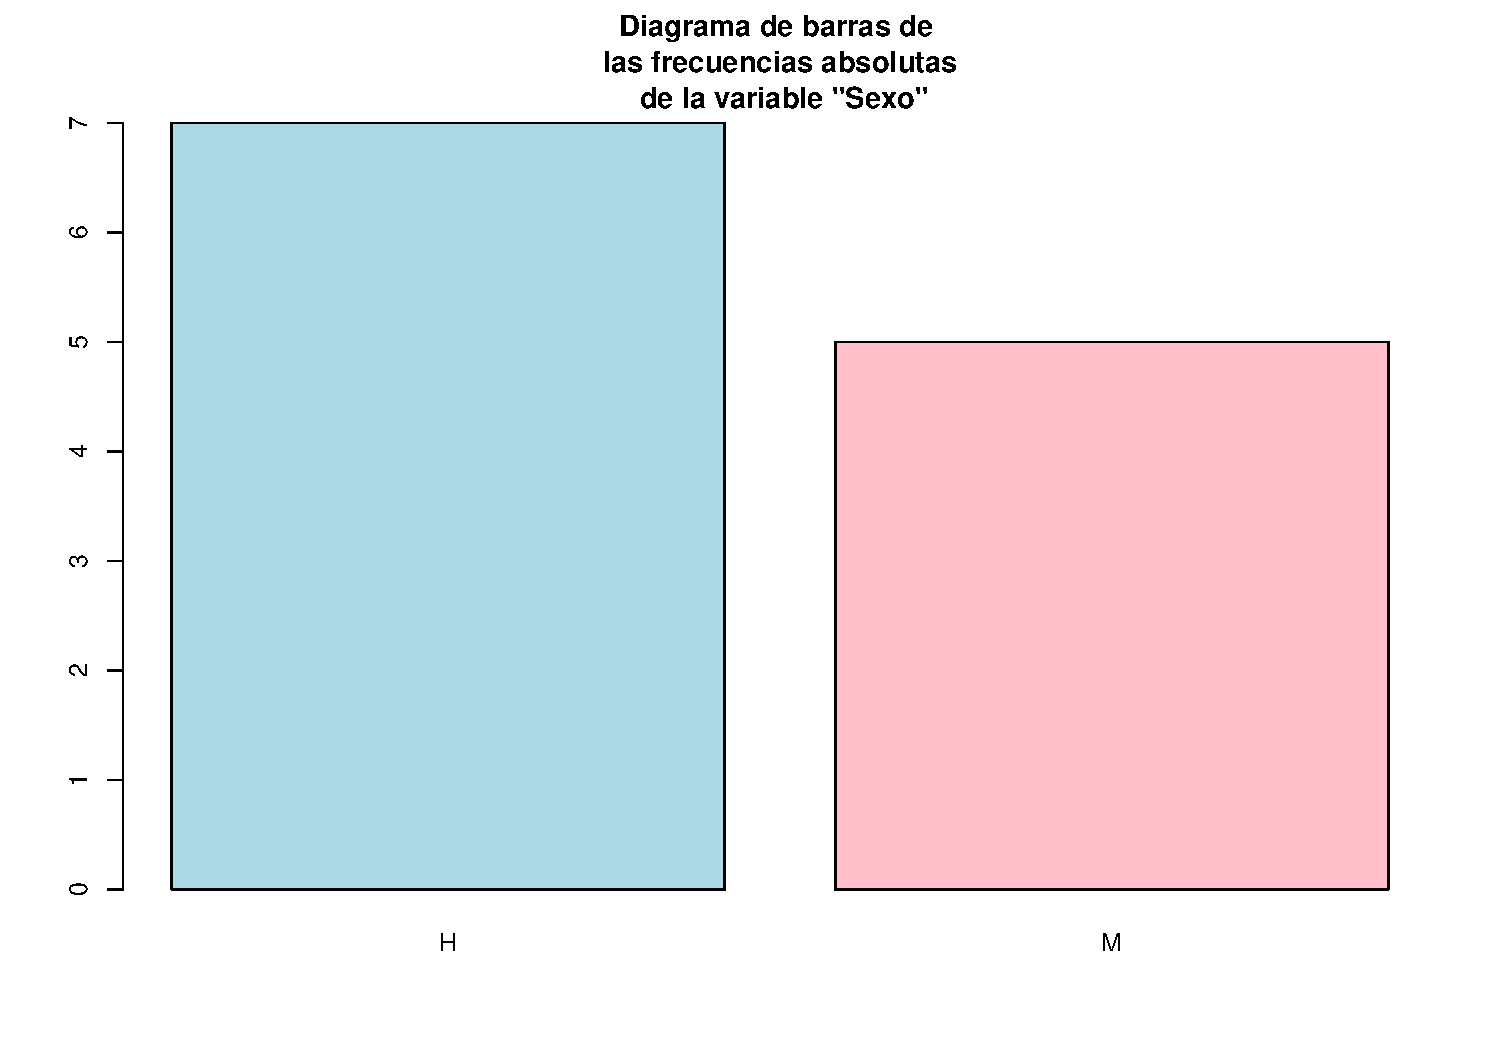
\includegraphics{R_base_files/figure-beamer/unnamed-chunk-85-1.pdf}
\end{frame}

\begin{frame}[fragile]{Diagrama de barras}
\phantomsection\label{diagrama-de-barras-2}
\begin{Shaded}
\begin{Highlighting}[]
\FunctionTok{barplot}\NormalTok{(}\FunctionTok{prop.table}\NormalTok{(}\FunctionTok{table}\NormalTok{(Respuestas)), }\AttributeTok{main=}\StringTok{"Diagrama de barras de frecuencias }
\StringTok{        relativas}\SpecialCharTok{\textbackslash{}n}\StringTok{ de la variable }\SpecialCharTok{\textbackslash{}"}\StringTok{Respuestas}\SpecialCharTok{\textbackslash{}"}\StringTok{"}\NormalTok{)}
\end{Highlighting}
\end{Shaded}

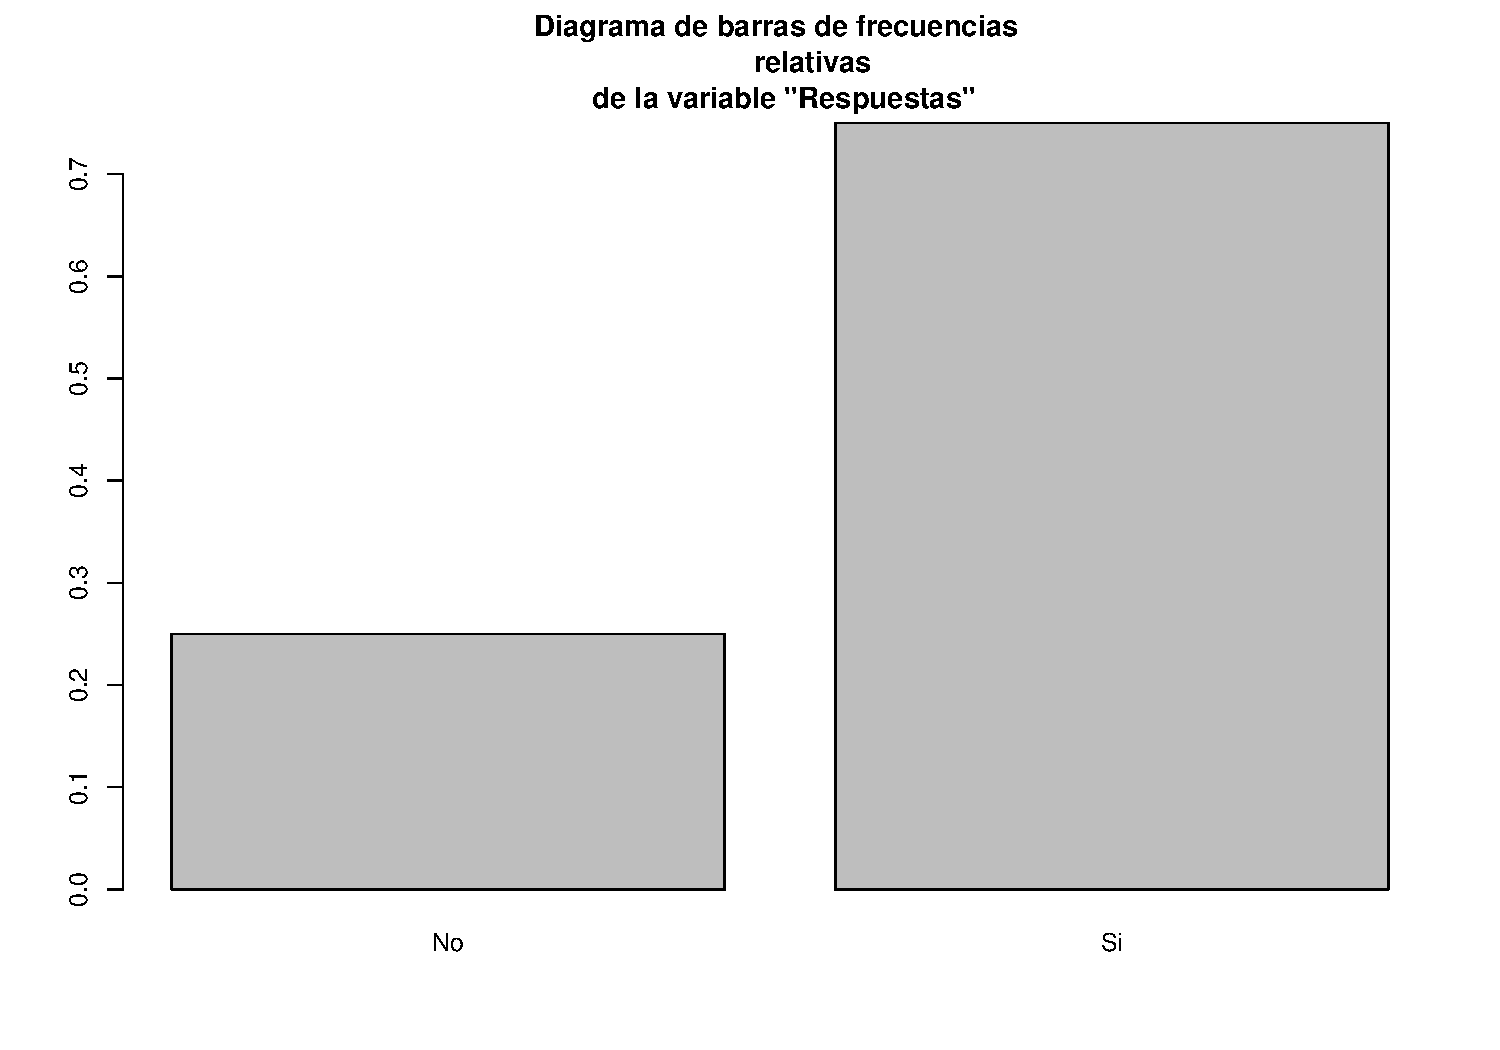
\includegraphics{R_base_files/figure-beamer/unnamed-chunk-86-1.pdf}
\end{frame}

\begin{frame}[fragile]{Diagrama de barras - Parámetros}
\phantomsection\label{diagrama-de-barras---paruxe1metros}
Habréis observado que en las funciones \texttt{barplot()} anteriores
hemos usado el parámetro \texttt{main} para poner título a los
diagramas; en general, la función \texttt{barplot()} admite los
parámetros de \texttt{plot} que tienen sentido en el contexto de los
diagramas de barras: \texttt{xlab}, \texttt{ylab}, \texttt{main}, etc.
Los parámetros disponibles se pueden consultar en
\texttt{help(barplot)}. Aquí sólo vamos a comentar algunos.
\end{frame}

\begin{frame}[fragile]{Diagrama de barras - Colores}
\phantomsection\label{diagrama-de-barras---colores}
\begin{Shaded}
\begin{Highlighting}[]
\FunctionTok{par}\NormalTok{(}\AttributeTok{mfrow=}\FunctionTok{c}\NormalTok{(}\DecValTok{1}\NormalTok{,}\DecValTok{2}\NormalTok{))}
\FunctionTok{barplot}\NormalTok{(}\FunctionTok{table}\NormalTok{(Respuestas), }\AttributeTok{col=}\FunctionTok{c}\NormalTok{(}\StringTok{"green"}\NormalTok{))}
\FunctionTok{barplot}\NormalTok{(}\FunctionTok{table}\NormalTok{(Respuestas), }\AttributeTok{col=}\FunctionTok{c}\NormalTok{(}\StringTok{"red"}\NormalTok{,}\StringTok{"blue"}\NormalTok{))}
\end{Highlighting}
\end{Shaded}

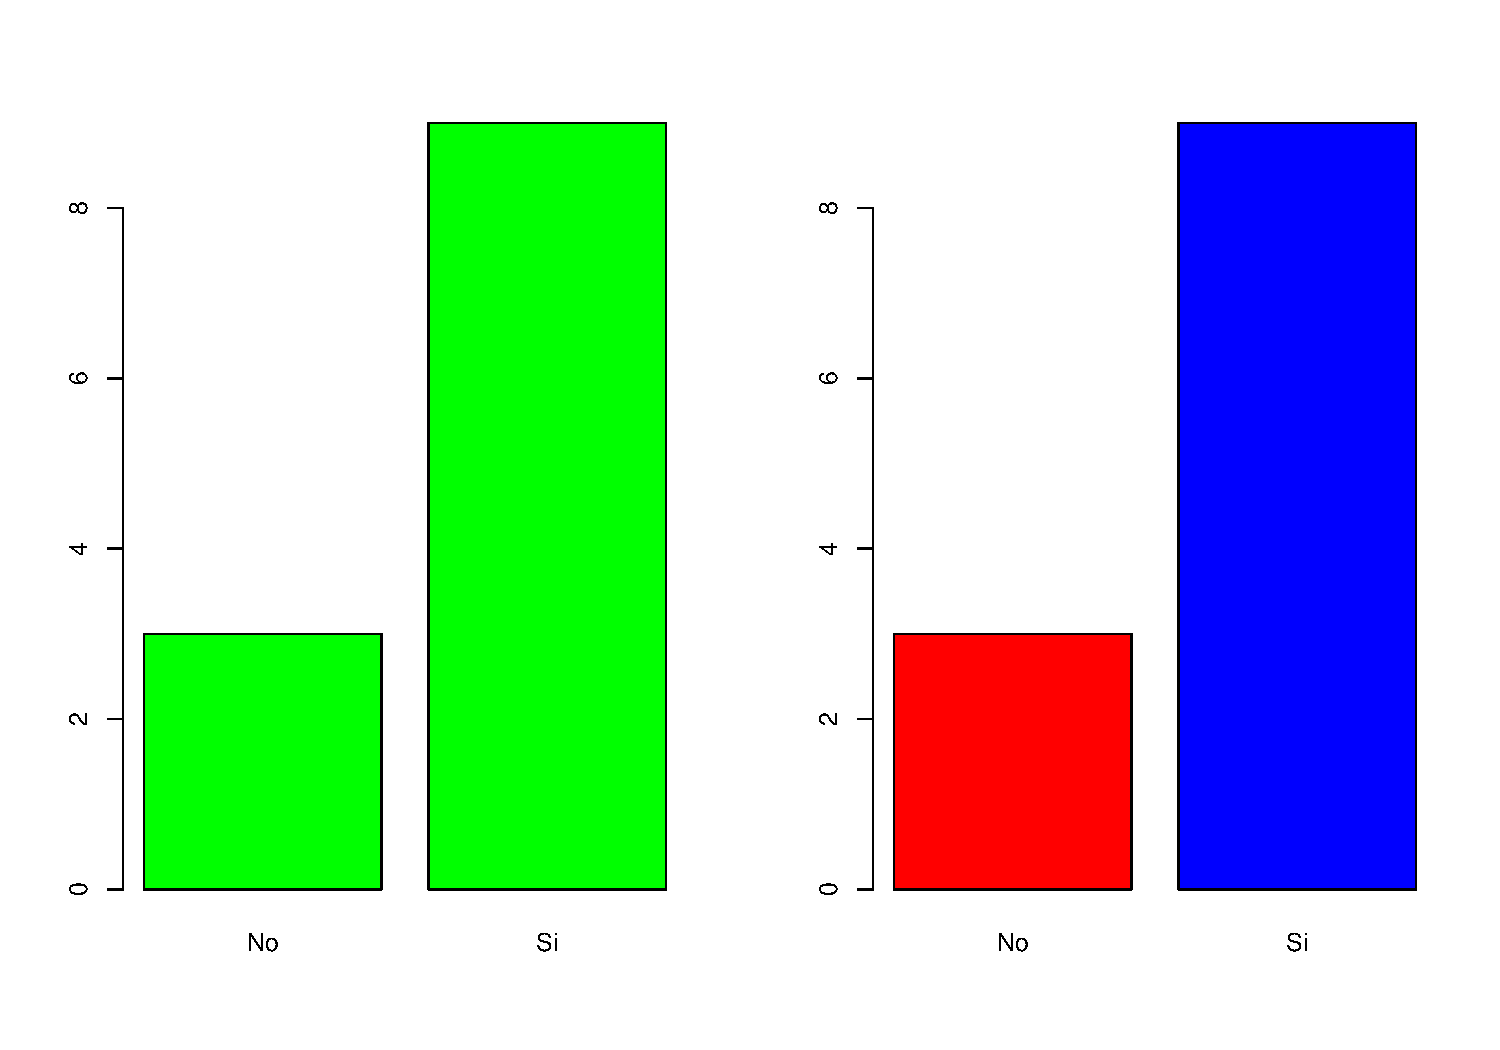
\includegraphics{R_base_files/figure-beamer/unnamed-chunk-87-1.pdf}

\begin{Shaded}
\begin{Highlighting}[]
\FunctionTok{par}\NormalTok{(}\AttributeTok{mfrow=}\FunctionTok{c}\NormalTok{(}\DecValTok{1}\NormalTok{,}\DecValTok{1}\NormalTok{))}
\end{Highlighting}
\end{Shaded}
\end{frame}

\begin{frame}[fragile]{Diagrama de barras - Colores}
\phantomsection\label{diagrama-de-barras---colores-1}
\begin{Shaded}
\begin{Highlighting}[]
\FunctionTok{barplot}\NormalTok{(}\FunctionTok{table}\NormalTok{(x), }\AttributeTok{horiz=}\ConstantTok{TRUE}\NormalTok{)}
\end{Highlighting}
\end{Shaded}

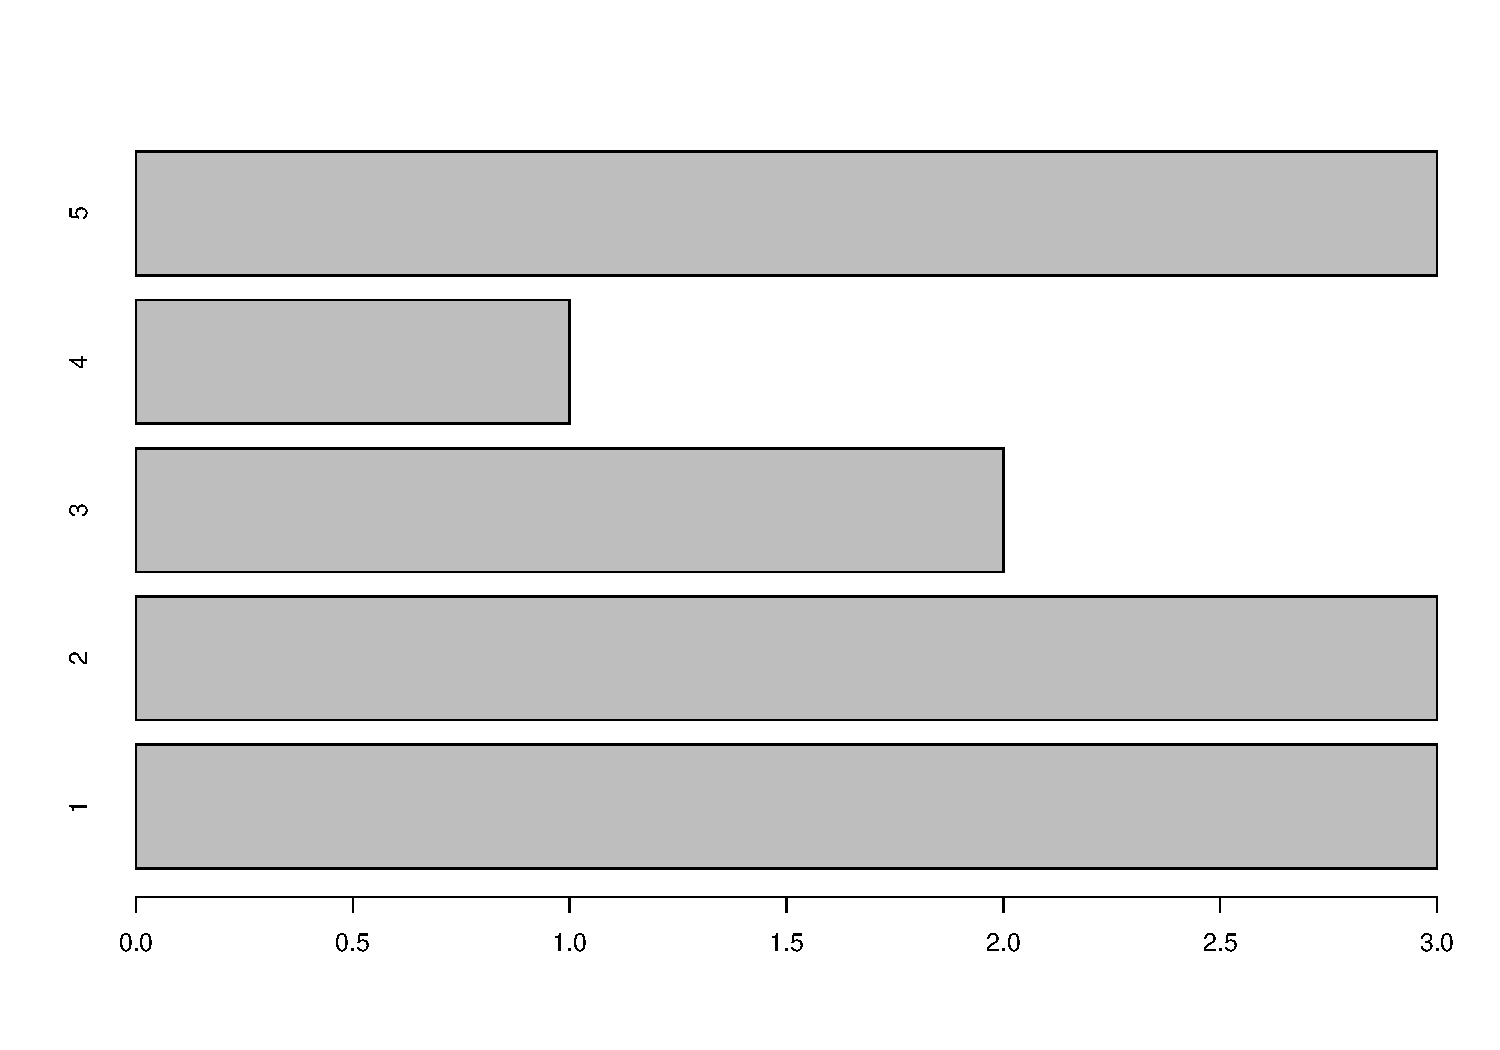
\includegraphics{R_base_files/figure-beamer/unnamed-chunk-88-1.pdf}
\end{frame}

\begin{frame}[fragile]{Diagrama de barras - Tabla bidimensional}
\phantomsection\label{diagrama-de-barras---tabla-bidimensional}
\begin{Shaded}
\begin{Highlighting}[]
\FunctionTok{barplot}\NormalTok{(}\FunctionTok{table}\NormalTok{(Sexo,Respuestas), }\AttributeTok{legend.text =} \ConstantTok{TRUE}\NormalTok{)}
\end{Highlighting}
\end{Shaded}

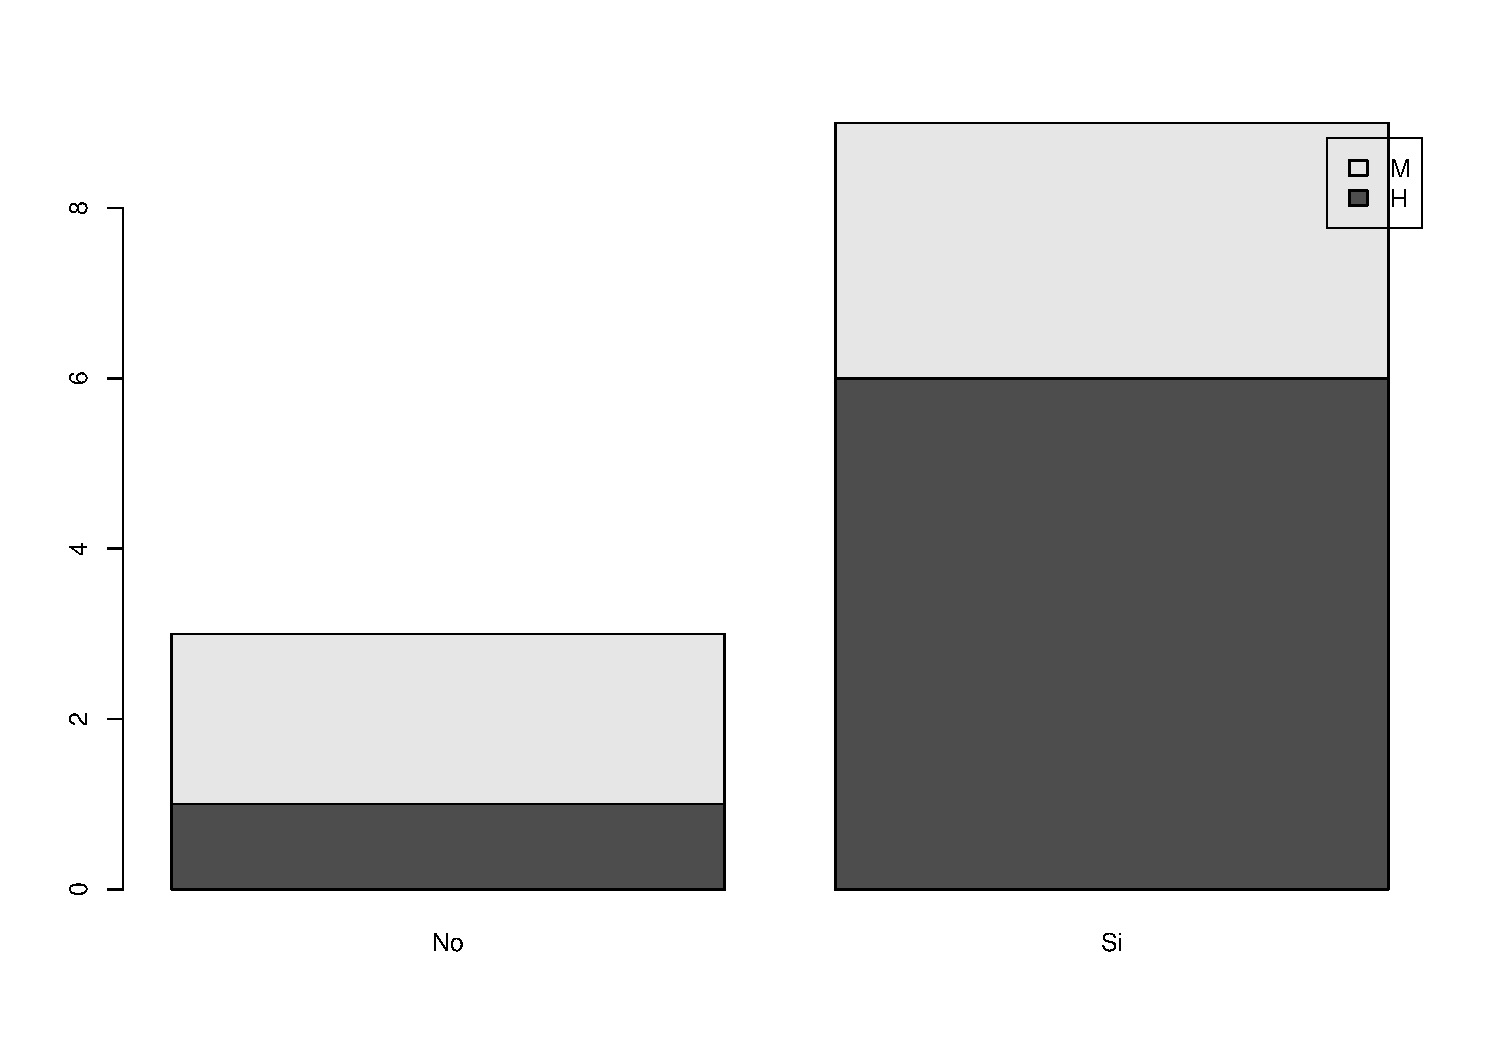
\includegraphics{R_base_files/figure-beamer/unnamed-chunk-89-1.pdf}
\end{frame}

\begin{frame}[fragile]{Diagrama de barras - Tabla bidimensional}
\phantomsection\label{diagrama-de-barras---tabla-bidimensional-1}
\begin{Shaded}
\begin{Highlighting}[]
\FunctionTok{barplot}\NormalTok{(}\FunctionTok{table}\NormalTok{(Sexo,Respuestas), }\AttributeTok{beside=}\ConstantTok{TRUE}\NormalTok{, }\AttributeTok{legend.text=}\ConstantTok{TRUE}\NormalTok{)}
\end{Highlighting}
\end{Shaded}

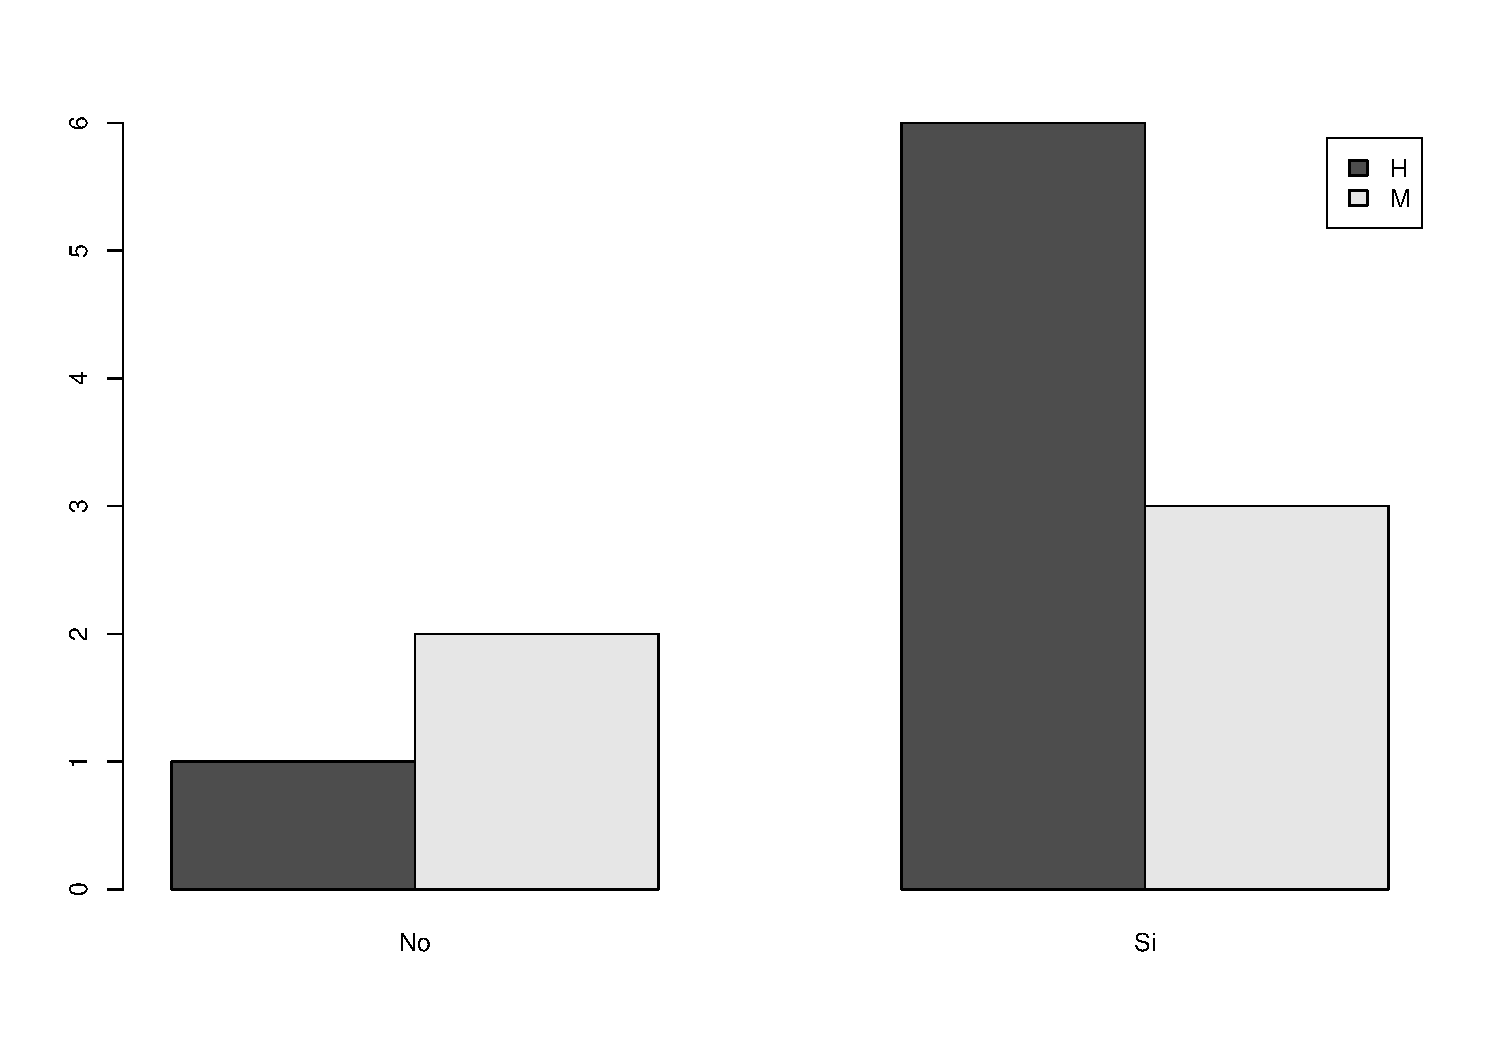
\includegraphics{R_base_files/figure-beamer/unnamed-chunk-90-1.pdf}
\end{frame}

\begin{frame}[fragile]{Diagrama de barras - Parámetros de las leyendas}
\phantomsection\label{diagrama-de-barras---paruxe1metros-de-las-leyendas}
\begin{Shaded}
\begin{Highlighting}[]
\FunctionTok{barplot}\NormalTok{(}\FunctionTok{table}\NormalTok{(Respuestas,Sexo), }\AttributeTok{beside=}\ConstantTok{TRUE}\NormalTok{, }\AttributeTok{names=}\FunctionTok{c}\NormalTok{(}\StringTok{"Men"}\NormalTok{, }\StringTok{"Women"}\NormalTok{), }
        \AttributeTok{col=}\FunctionTok{c}\NormalTok{(}\StringTok{"yellow"}\NormalTok{,}\StringTok{"lightblue"}\NormalTok{), }\AttributeTok{legend.text=}\FunctionTok{c}\NormalTok{(}\StringTok{"No"}\NormalTok{,}\StringTok{"Yes"}\NormalTok{))}
\end{Highlighting}
\end{Shaded}

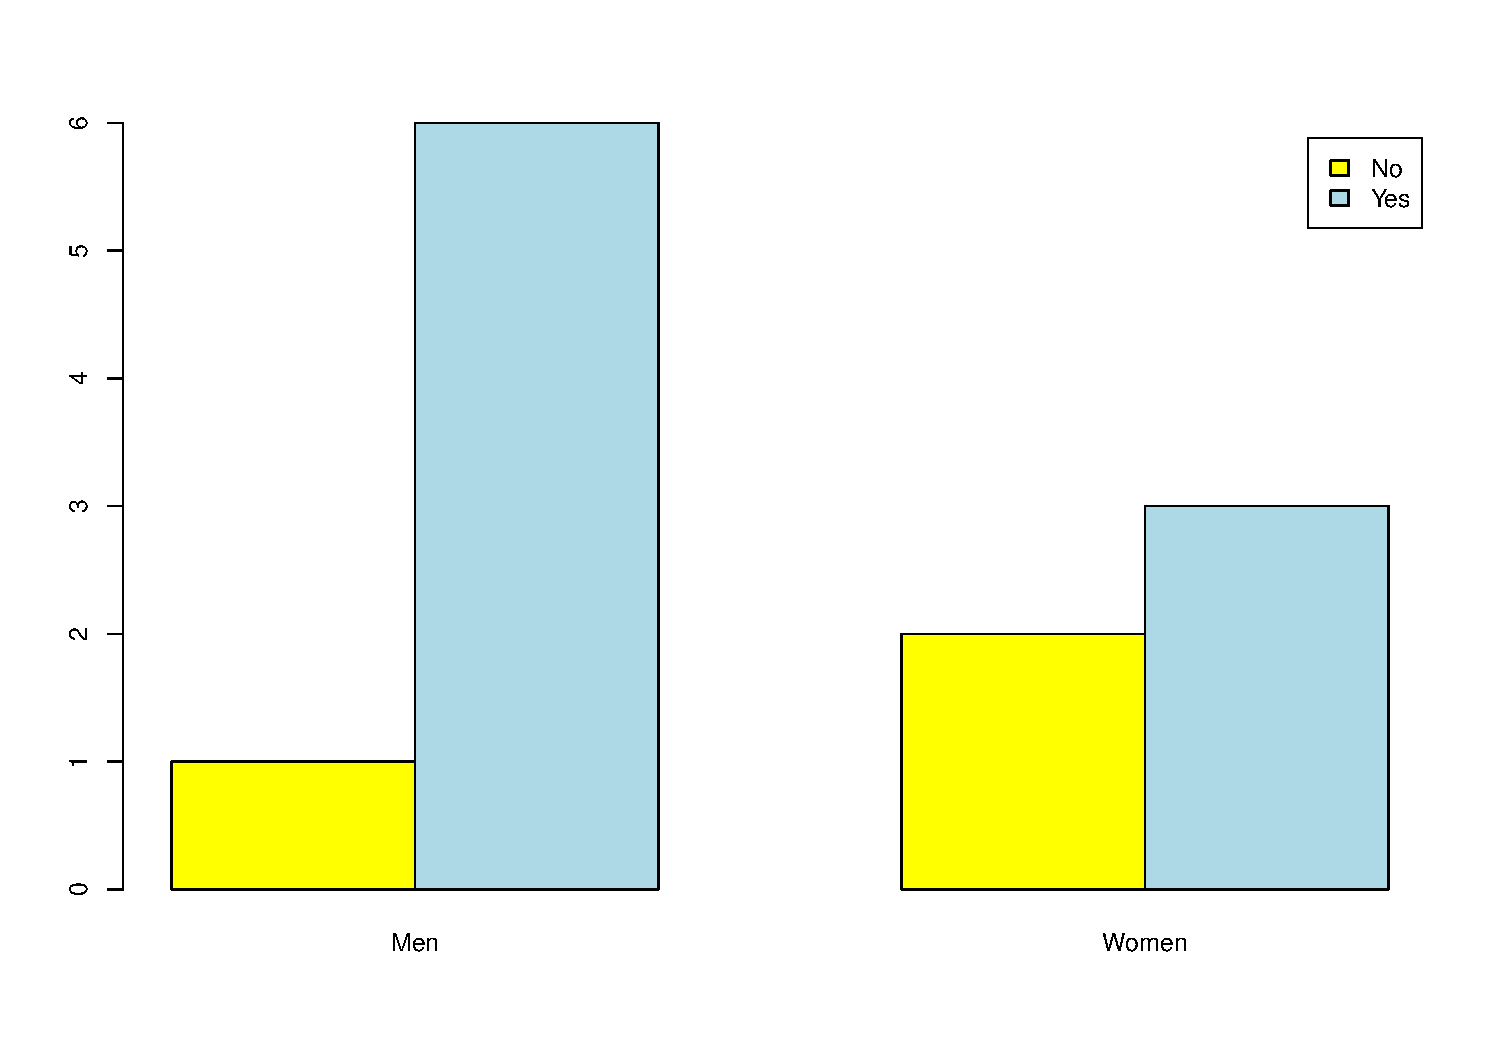
\includegraphics{R_base_files/figure-beamer/unnamed-chunk-91-1.pdf}
\end{frame}

\begin{frame}[fragile]{Diagrama circular}
\phantomsection\label{diagrama-circular}
Un tipo muy popular de representación gráfica de variables cualitativas
son los \blue{diagramas circulares}. En un diagrama circular
(\texttt{pie\ chart}) se representan los niveles de una variable
cualitativa como sectores circulares de un círculo, de manera que el
ángulo (o equivalentemente, el área) de cada sector sea proporcional a
la frecuencia del nivel al que corresponde.

Con R, este tipo de diagramas se producen con la instrucción
\texttt{pie}, de nuevo aplicada a una tabla de frecuencias y no al
vector original.
\end{frame}

\begin{frame}[fragile]{Diagrama circular - Parámetros}
\phantomsection\label{diagrama-circular---paruxe1metros}
La función \texttt{pie} admite muchos parámetros para modificar el
resultado: se pueden cambiar los colores con \texttt{col}, se pueden
cambiar los nombres de los niveles con \texttt{names}, se puede poner un
título con \texttt{main}, etc.; podéis consultar la lista completa de
parámetros en \texttt{help(pie)}.
\end{frame}

\begin{frame}[fragile]{Diagrama circular}
\phantomsection\label{diagrama-circular-1}
\begin{Shaded}
\begin{Highlighting}[]
\NormalTok{x}
\end{Highlighting}
\end{Shaded}

\begin{verbatim}
 [1] 1 1 5 2 2 2 1 4 5 3 3 5
\end{verbatim}

\begin{Shaded}
\begin{Highlighting}[]
\FunctionTok{pie}\NormalTok{(}\FunctionTok{table}\NormalTok{(x), }\AttributeTok{main=}\StringTok{"Diagrama circular de la variable x"}\NormalTok{)}
\end{Highlighting}
\end{Shaded}

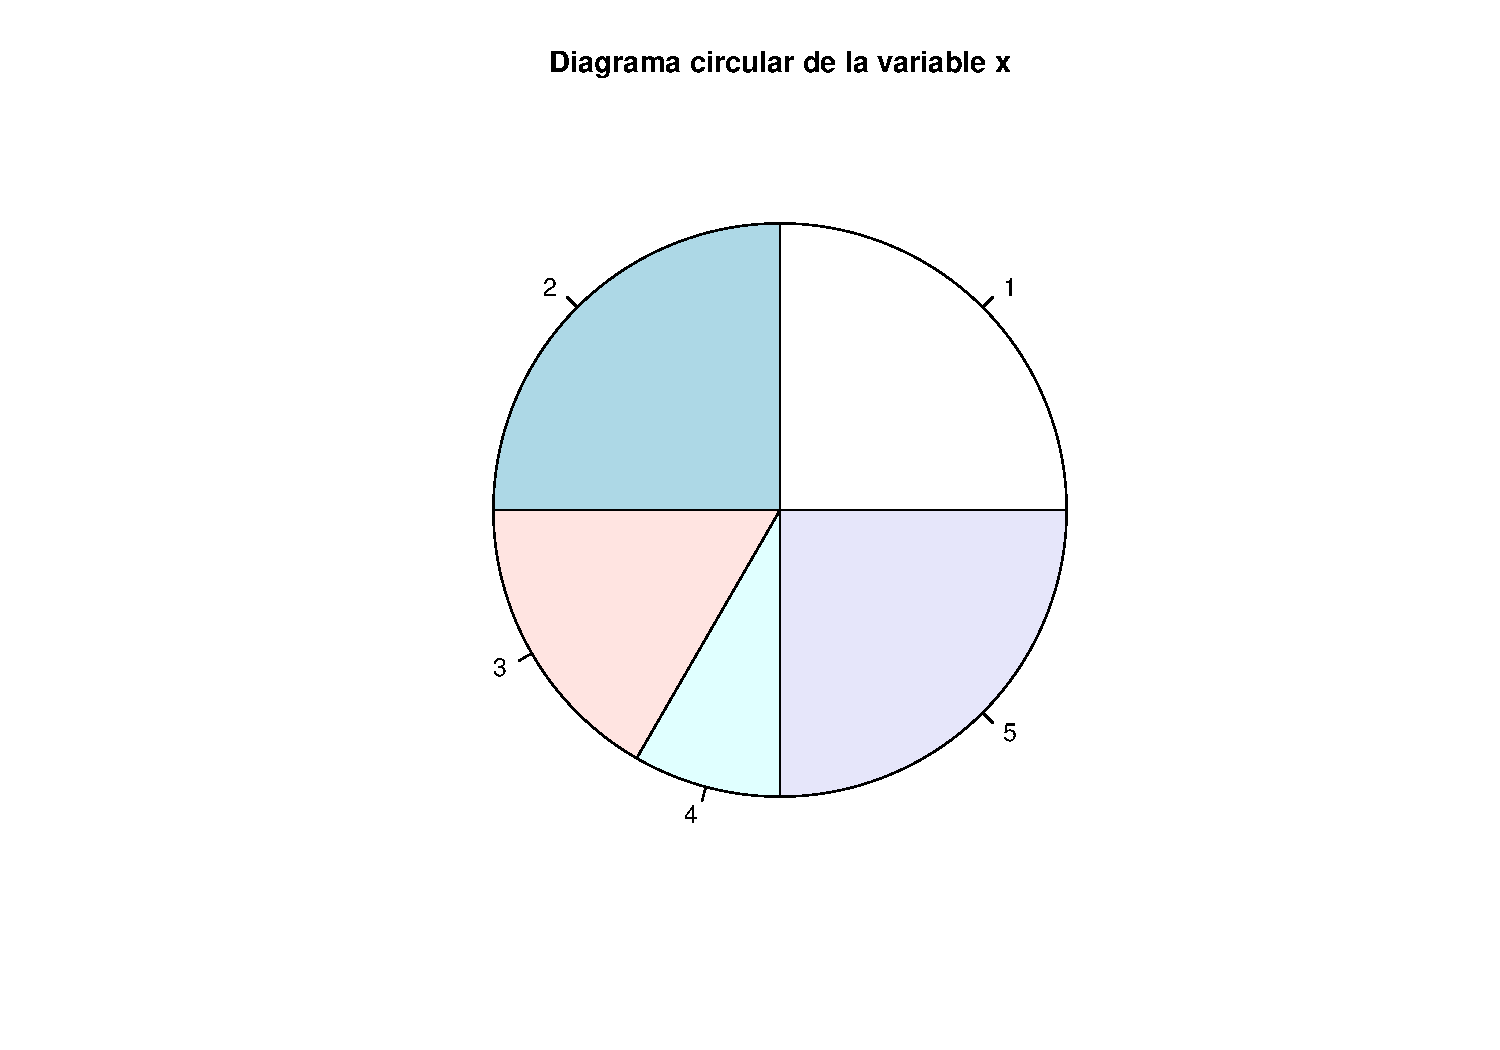
\includegraphics{R_base_files/figure-beamer/unnamed-chunk-92-1.pdf}
\end{frame}

\begin{frame}[fragile]{Diagrama circular}
\phantomsection\label{diagrama-circular-2}
\begin{Shaded}
\begin{Highlighting}[]
\NormalTok{Respuestas}
\end{Highlighting}
\end{Shaded}

\begin{verbatim}
 [1] Si Si No Si Si Si Si Si No Si No Si
Levels: No Si
\end{verbatim}

\begin{Shaded}
\begin{Highlighting}[]
\FunctionTok{pie}\NormalTok{(}\FunctionTok{table}\NormalTok{(Respuestas), }\AttributeTok{main=}\StringTok{"Diagrama circular de la variable Respuestas"}\NormalTok{)}
\end{Highlighting}
\end{Shaded}

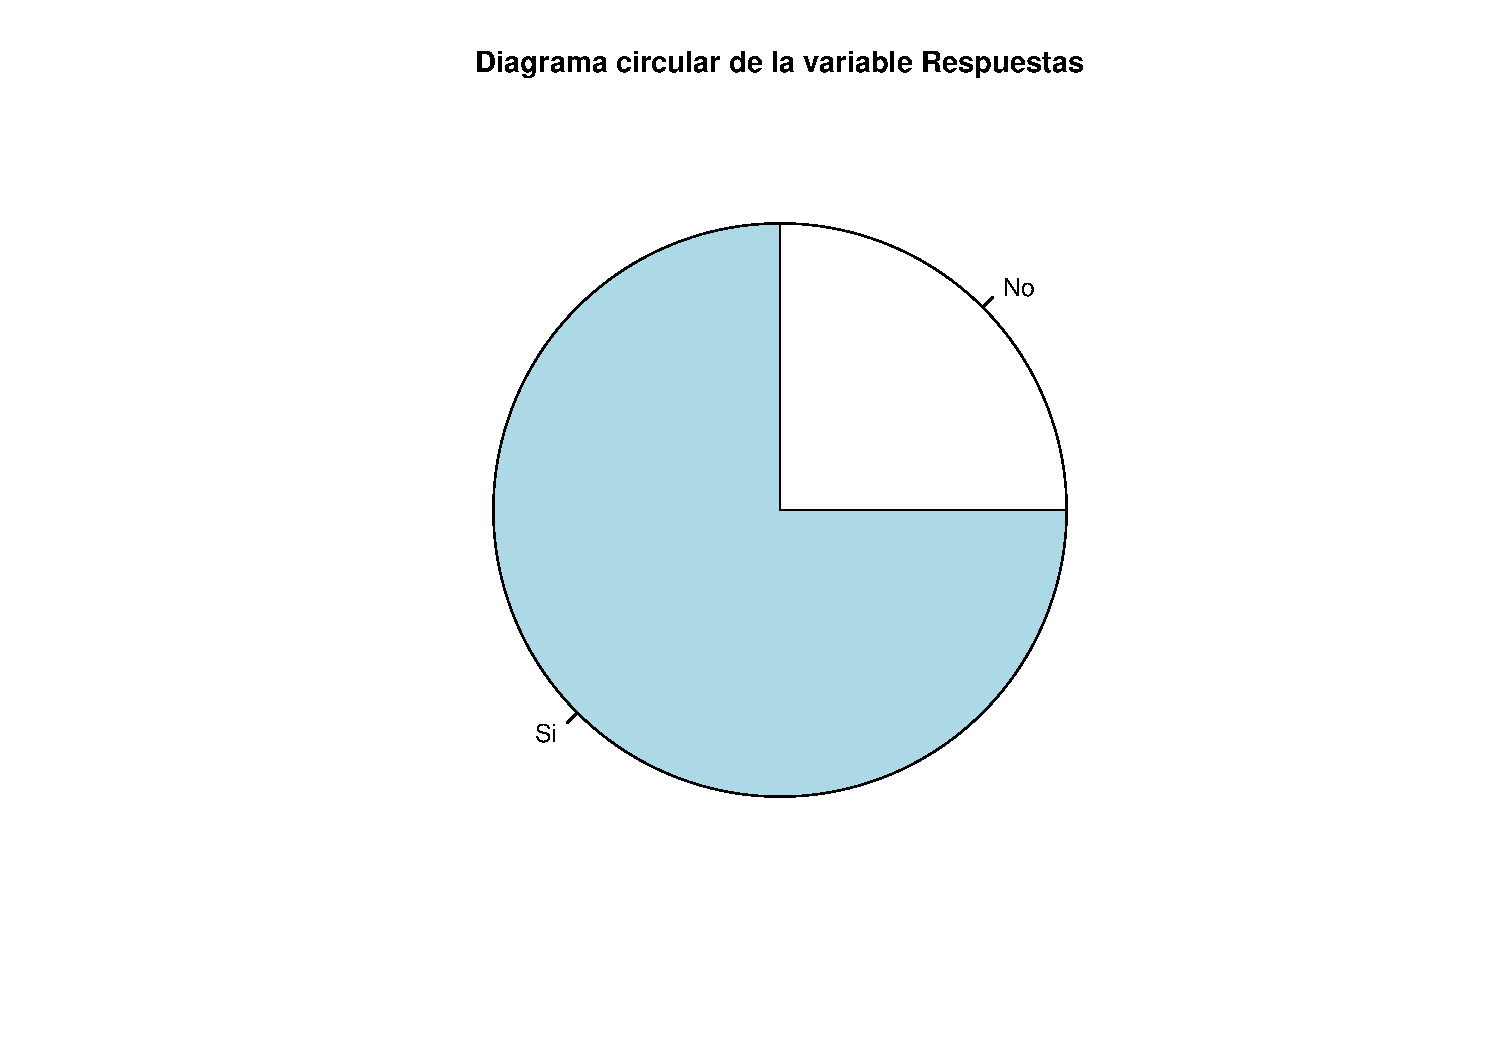
\includegraphics{R_base_files/figure-beamer/unnamed-chunk-93-1.pdf}
\end{frame}

\begin{frame}{Diagrama circular}
\phantomsection\label{diagrama-circular-3}
Pese a su popularidad, es poco recomendable usar diagramas circulares
porque a veces es difícil, a simple vista, comprender las relaciones
entre las frecuencias que representan.
\end{frame}

\begin{frame}[fragile]{Gráficos de mosaico}
\phantomsection\label{gruxe1ficos-de-mosaico}
Otra representación de las tablas multidimensionales de frecuencias son
los \blue{gráficos de mosaico}. Estos gráficos se obtienen sustituyendo
cada entrada de la tabla de frecuencias por una región rectangular de
área proporcional a su valor.

En concreto, para obtener el gráfico de mosaico de una tabla
bidimensional, se parte de un cuadrado de lado 1, primero se divide en
barras verticales de amplitudes iguales a las frecuencias relativas de
una variable, y luego cada barra se divide, a lo alto, en regiones de
alturas proporcionales a las frecuencias relativas marginales de cada
nivel de la otra variable, dentro del nivel correspondiente de la
primera variable.

Un gráfico de mosaico de una tabla se obtiene con R aplicando la función
\texttt{plot} a la tabla, o también la función \texttt{mosaicplot}. Esta
última también se puede aplicar a matrices.
\end{frame}

\begin{frame}[fragile]{Gráficos de mosaico}
\phantomsection\label{gruxe1ficos-de-mosaico-1}
\begin{Shaded}
\begin{Highlighting}[]
\FunctionTok{plot}\NormalTok{(}\FunctionTok{table}\NormalTok{(Sexo,Respuestas), }\AttributeTok{main=}\StringTok{"Gráfico de mosaico de las variables}
\StringTok{     }\SpecialCharTok{\textbackslash{}"}\StringTok{Sexo}\SpecialCharTok{\textbackslash{}"}\StringTok{ y }\SpecialCharTok{\textbackslash{}"}\StringTok{Respuestas}\SpecialCharTok{\textbackslash{}"}\StringTok{"}\NormalTok{)}
\end{Highlighting}
\end{Shaded}

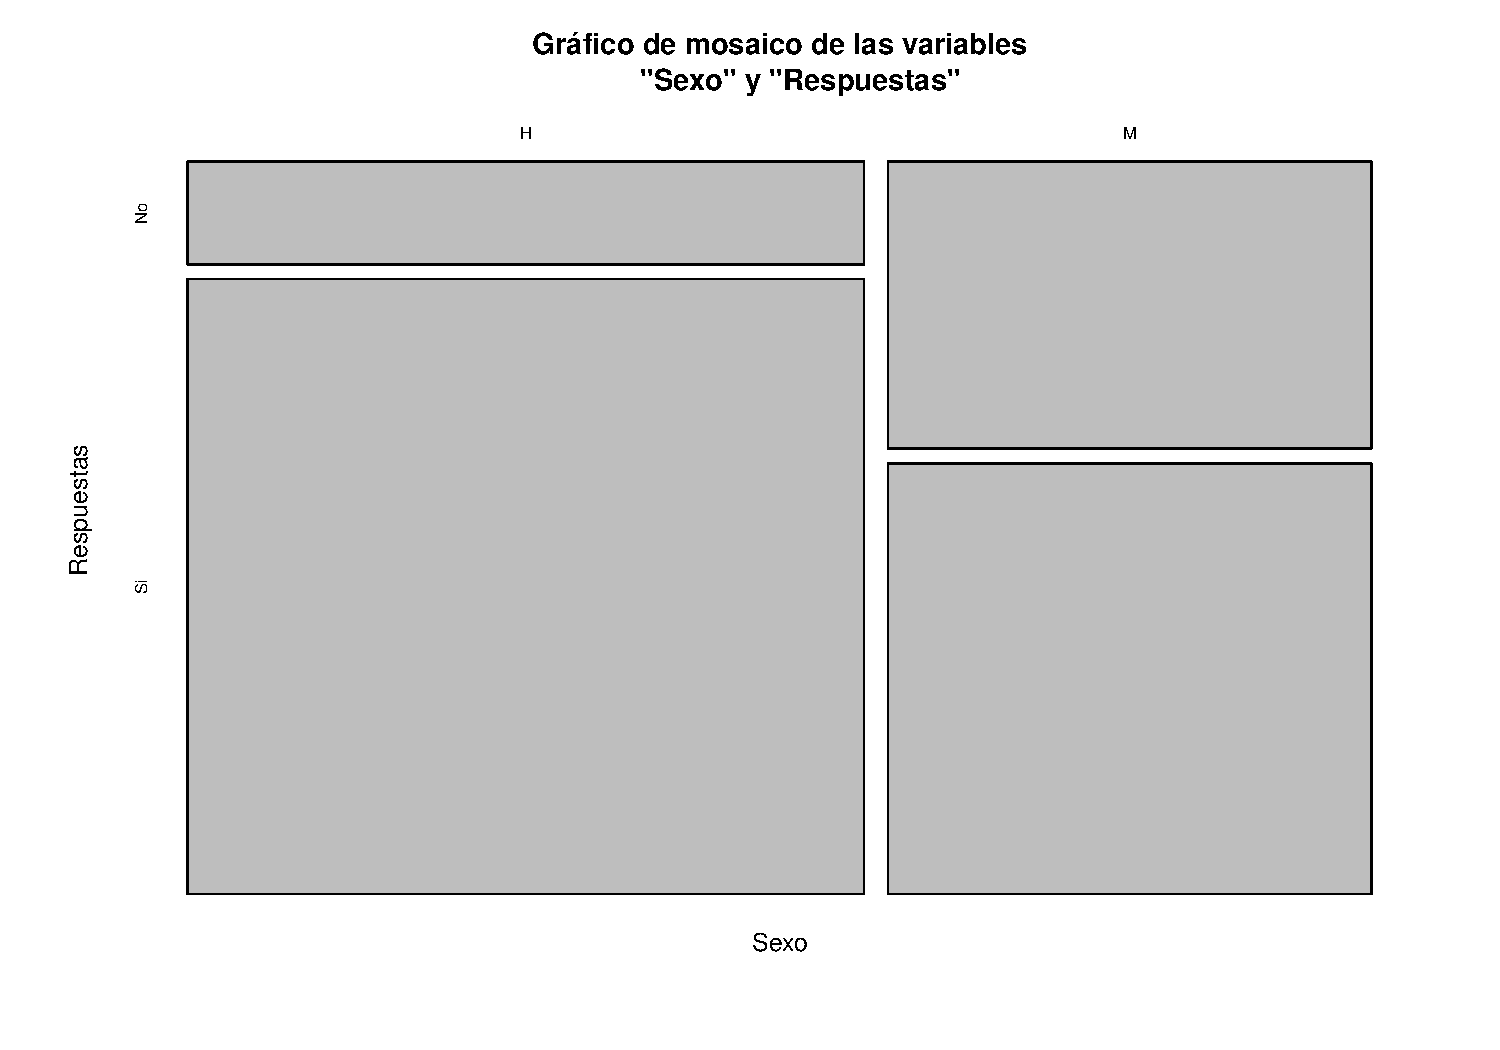
\includegraphics{R_base_files/figure-beamer/unnamed-chunk-94-1.pdf}
\end{frame}

\begin{frame}{Gráficos de mosaico}
\phantomsection\label{gruxe1ficos-de-mosaico-2}
En el gráfico de mosaico de una tabla tridimensional, primero se divide
el cuadrado en barras verticales de amplitudes iguales a las frecuencias
relativas de una variable.

Luego cada barra se divide, a lo alto, en regiones de alturas
proporcionales a las frecuencias relativas marginales de cada nivel de
una segunda variable, dentro del nivel correspondiente de la primera
variable.

Finalmente, cada sector rectangular se vuelve a dividir a lo ancho en
regiones de amplitudes proporcionales a las frecuencias relativas
marginales de cada nivel de la tercera variable dentro de la combinación
correspondiente de niveles de las otras dos.
\end{frame}

\begin{frame}[fragile]{Gráficos de mosaico}
\phantomsection\label{gruxe1ficos-de-mosaico-3}
\begin{Shaded}
\begin{Highlighting}[]
\FunctionTok{plot}\NormalTok{(HairEyeColor, }\AttributeTok{main=}\StringTok{"Gráfico de mosaico de la tabla HairEyeColor"}\NormalTok{, }
     \AttributeTok{col=}\FunctionTok{c}\NormalTok{(}\StringTok{"pink"}\NormalTok{,}\StringTok{"lightblue"}\NormalTok{))}
\end{Highlighting}
\end{Shaded}

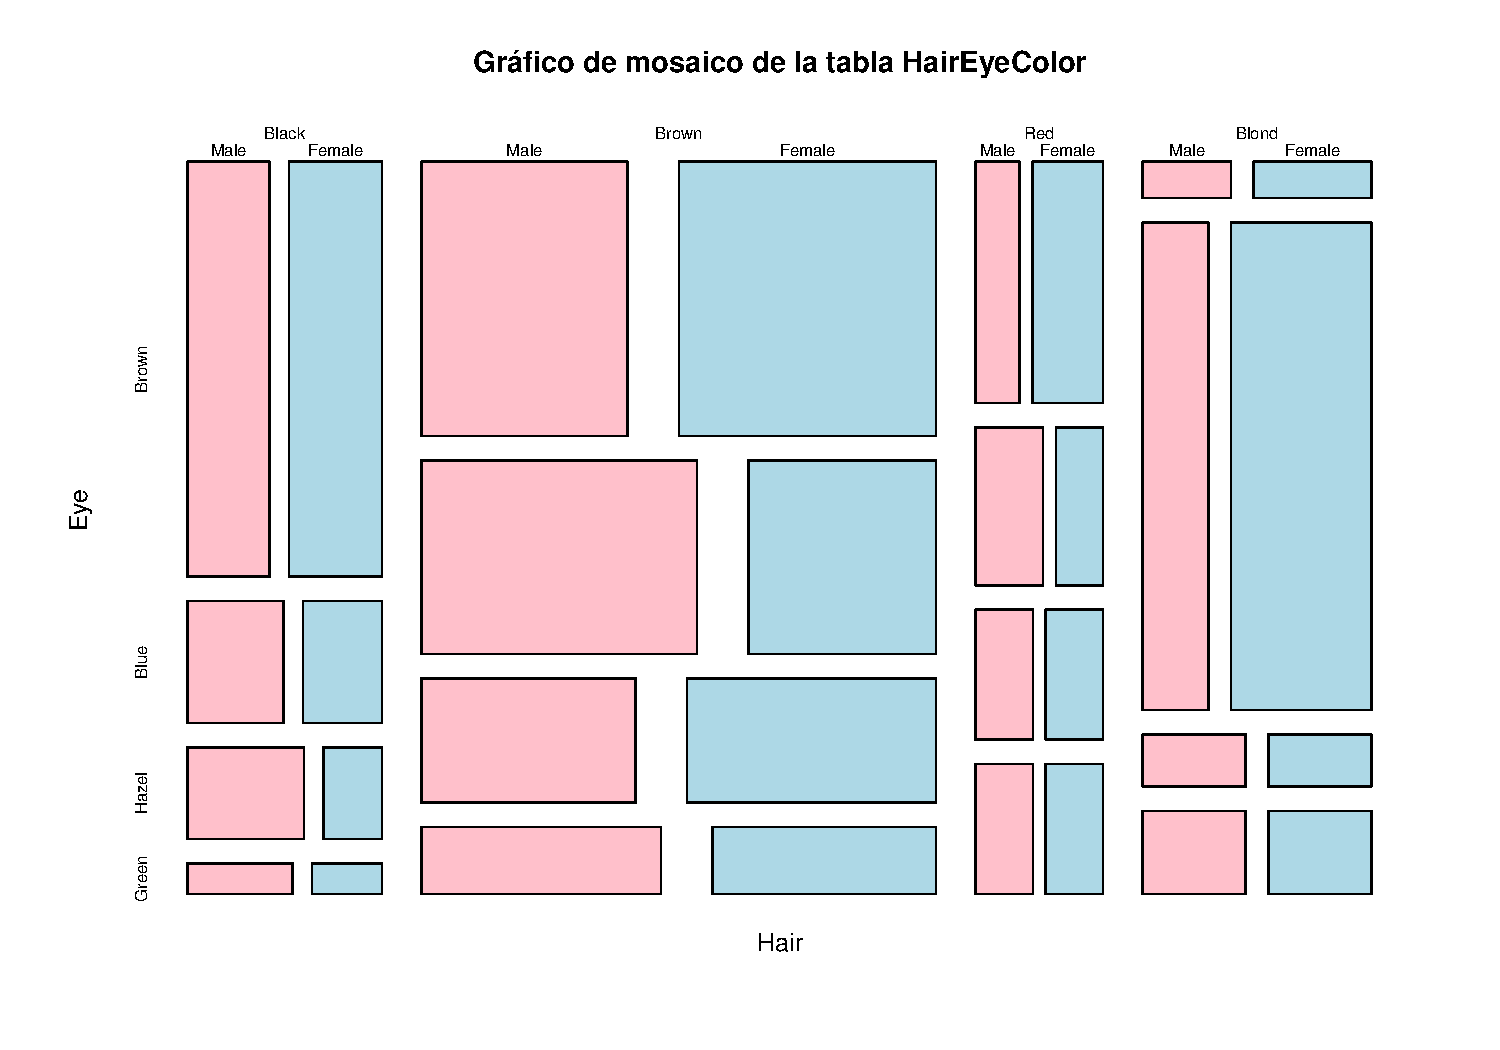
\includegraphics{R_base_files/figure-beamer/unnamed-chunk-95-1.pdf}
\end{frame}

\begin{frame}[fragile]{Muchos más gráficos}
\phantomsection\label{muchos-muxe1s-gruxe1ficos}
Además de sus parámetros usuales, la función \texttt{plot} admite
algunos parámetros específicos cuando se usa para producir el gráfico de
mosaico de una tabla. Estos parámetros se pueden consultar en
\texttt{help(mosaicplot)}.

Los paquetes \texttt{vcd} y \texttt{vcdExtra} incluyen otras funciones
que producen representaciones gráficas interesantes de tablas
tridimensionales.

\begin{itemize}
\tightlist
\item
  La función \texttt{cotabplot} de \texttt{vcd} produce un diagrama de
  mosaico para cada nivel de la tercera variable.
\item
  La función \texttt{mosaic3d} de \texttt{vcdExtra} produce un diagrama
  de mosaico tridimensional en una ventana de una aplicación para
  gráficos 3D interactivos.
\end{itemize}
\end{frame}

\section{Ejemplo final}\label{ejemplo-final}

\begin{frame}[fragile]{Un ejemplo final}
\phantomsection\label{un-ejemplo-final}
Vamos a llevar a cabo un análisis completo de un ejemplo con lo que
hemos aprendido en esta lección y aprovecharemos para aprender algo
nuevo.

El objeto de datos \texttt{HairEyeColor} que lleva predefinido R es una
tabla de frecuencias absolutas de tres variables cualitativas: color de
cabello (\texttt{Hair}), color de los ojos (\texttt{Eye}) y sexo
(\texttt{Sex}).

Vamos a extraer de esta tabla una tabla bidimensional de frecuencias
absolutas de las variables \texttt{Eye} y \texttt{Hair}, sin distinguir
según el sexo. La manera más sencilla de obtener esta tabla es sumando
las subtablas de frecuencias para hombres y mujeres, y aplicando
\texttt{as.table()} al resultado para transformarlo en una
\texttt{table} por si no lo es.
\end{frame}

\begin{frame}[fragile]{Un ejemplo final}
\phantomsection\label{un-ejemplo-final-1}
Vamos a traducir al castellano los nombres de las variables de esta
tabla y de sus niveles. Esto lo podemos llevar a cabo en un solo paso
con la función \texttt{dimnames()} que ya usamos sobre data frames. El
resultado de aplicar esta función a una table es una \texttt{list} cuyas
componentes son los niveles de cada variable.

\begin{Shaded}
\begin{Highlighting}[]
\FunctionTok{dimnames}\NormalTok{(HEC)}
\end{Highlighting}
\end{Shaded}

\begin{verbatim}
$Hair
[1] "Black" "Brown" "Red"   "Blond"

$Eye
[1] "Brown" "Blue"  "Hazel" "Green"
\end{verbatim}

\textbf{Ejercicio.}

Redefinid dicha \texttt{list} para tener los niveles de los factores en
castellano
\end{frame}

\begin{frame}{Un ejemplo final}
\phantomsection\label{un-ejemplo-final-2}
Vamos a dibujar un diagrama de mosaico de esta tabla, para visualizar
gráficamente sus entradas.

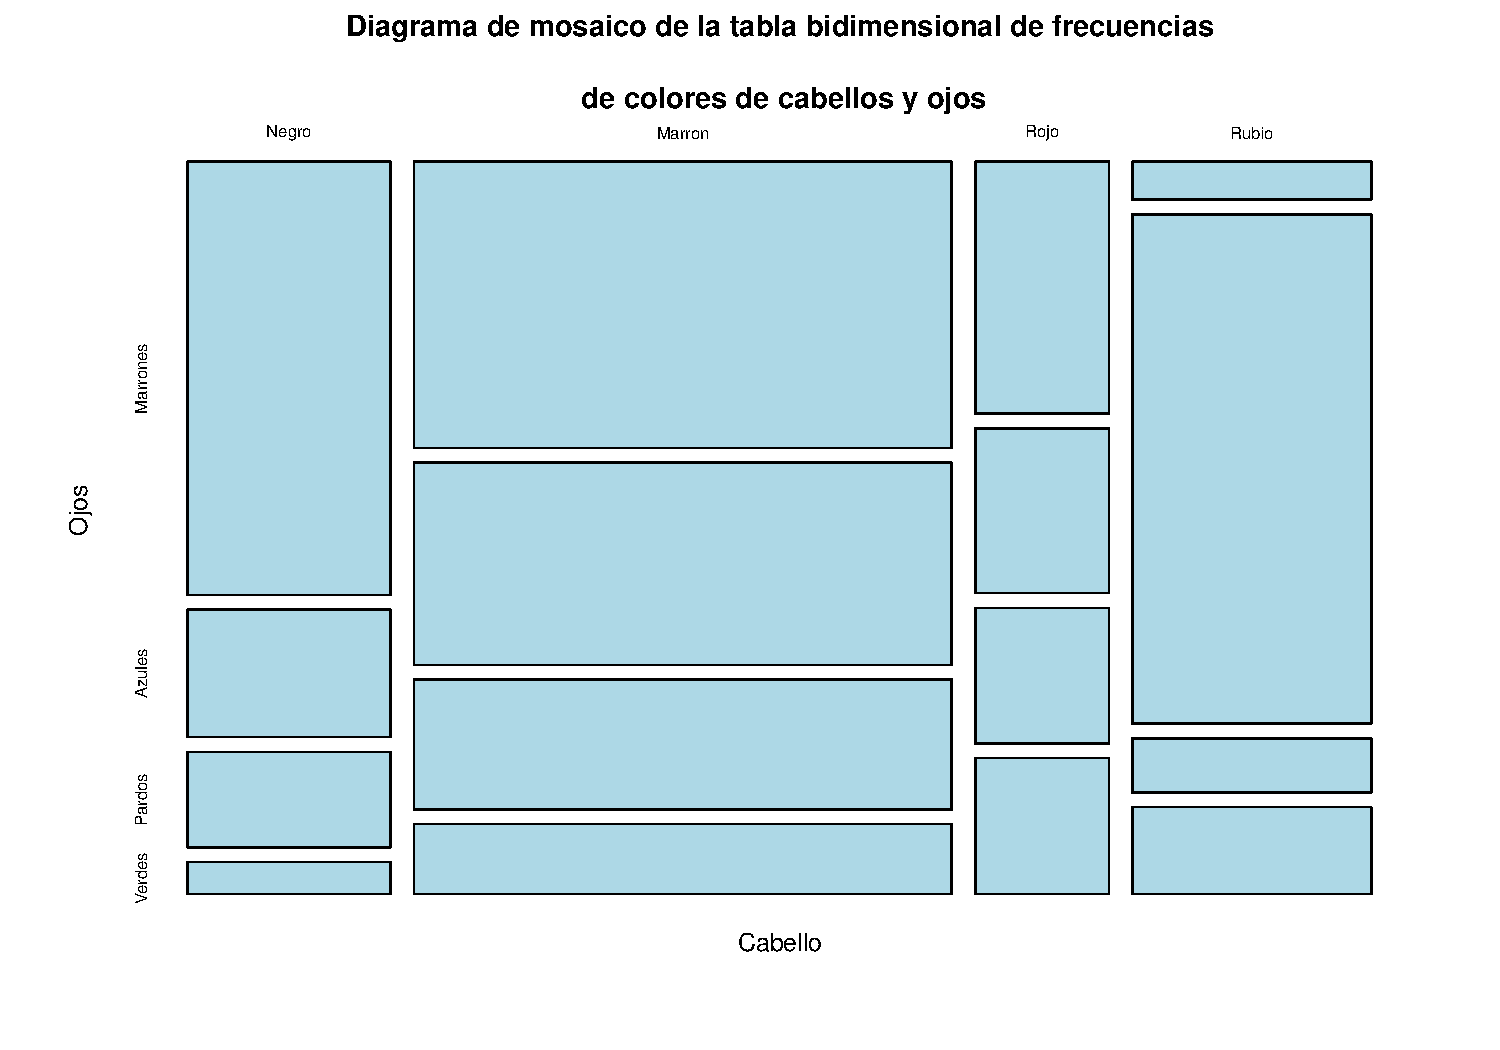
\includegraphics{R_base_files/figure-beamer/unnamed-chunk-101-1.pdf}
\end{frame}

\begin{frame}[fragile]{Un ejemplo final}
\phantomsection\label{un-ejemplo-final-3}
A continuación, vamos a calcular el número total de individuos
representados en esta tabla:

\begin{verbatim}
[1] 592
\end{verbatim}
\end{frame}

\begin{frame}[fragile]{Un ejemplo final}
\phantomsection\label{un-ejemplo-final-4}
Las tablas de frecuencias absolutas y relativas de cada variable,

\begin{verbatim}
Marrones   Azules   Pardos   Verdes 
     220      215       93       64 
\end{verbatim}

\begin{verbatim}
 Negro Marron   Rojo  Rubio 
   108    286     71    127 
\end{verbatim}

\begin{verbatim}
Marrones   Azules   Pardos   Verdes 
   0.372    0.363    0.157    0.108 
\end{verbatim}

\begin{verbatim}
 Negro Marron   Rojo  Rubio 
 0.182  0.483  0.120  0.215 
\end{verbatim}
\end{frame}

\begin{frame}{Un ejemplo final}
\phantomsection\label{un-ejemplo-final-5}
Representaremos estas últimas en sendos diagramas de barras.

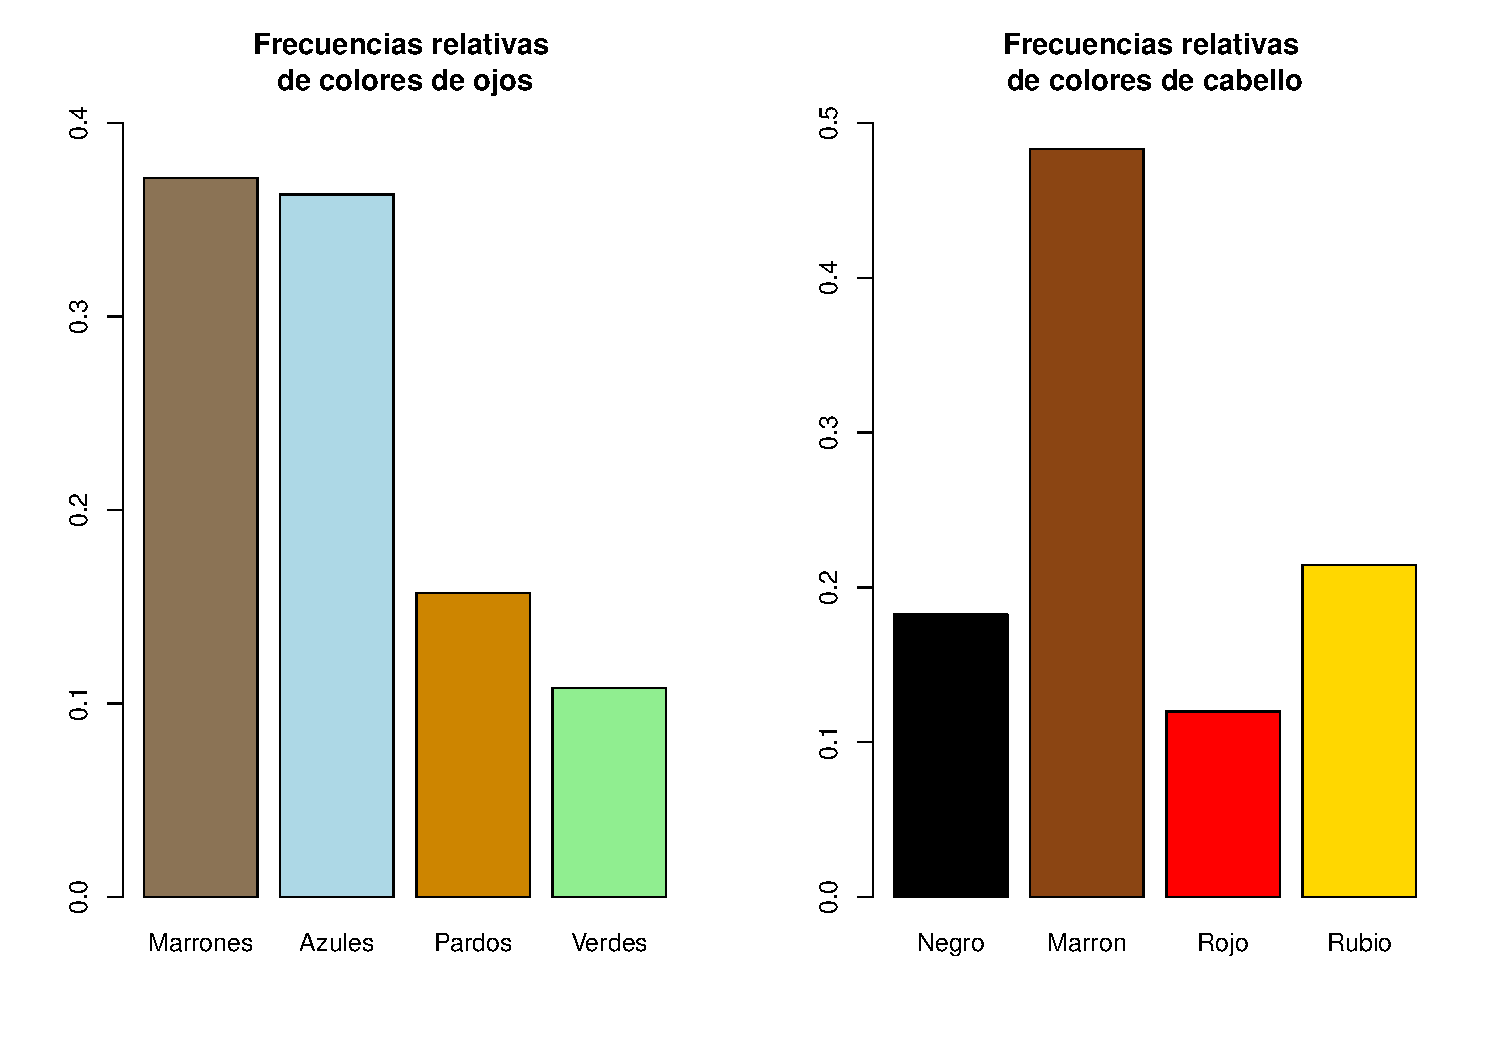
\includegraphics{R_base_files/figure-beamer/unnamed-chunk-104-1.pdf}
\end{frame}

\begin{frame}[fragile]{Un ejemplo final}
\phantomsection\label{un-ejemplo-final-6}
En el diagrama anterior vemos que el color dominante de cabellos es el
castaño, mientras que en el color de ojos el marrón y el azul están
prácticamente empatados. Pasamos ahora a calcular las tablas de
frecuencias relativas y dibujar los dos diagramas de barras de las
frecuencias relativas marginales.

\begin{verbatim}
        Ojos
Cabello  Marrones Azules Pardos Verdes
  Negro     0.115  0.034  0.025  0.008
  Marron    0.201  0.142  0.091  0.049
  Rojo      0.044  0.029  0.024  0.024
  Rubio     0.012  0.159  0.017  0.027
\end{verbatim}
\end{frame}

\begin{frame}[fragile]{Un ejemplo final}
\phantomsection\label{un-ejemplo-final-7}
\begin{verbatim}
        Ojos
Cabello  Marrones Azules Pardos Verdes
  Negro     0.630  0.185  0.139  0.046
  Marron    0.416  0.294  0.189  0.101
  Rojo      0.366  0.239  0.197  0.197
  Rubio     0.055  0.740  0.079  0.126
\end{verbatim}

\begin{verbatim}
        Ojos
Cabello  Marrones Azules Pardos Verdes
  Negro     0.309  0.093  0.161  0.078
  Marron    0.541  0.391  0.581  0.453
  Rojo      0.118  0.079  0.151  0.219
  Rubio     0.032  0.437  0.108  0.250
\end{verbatim}
\end{frame}

\begin{frame}{Un ejemplo final}
\phantomsection\label{un-ejemplo-final-8}
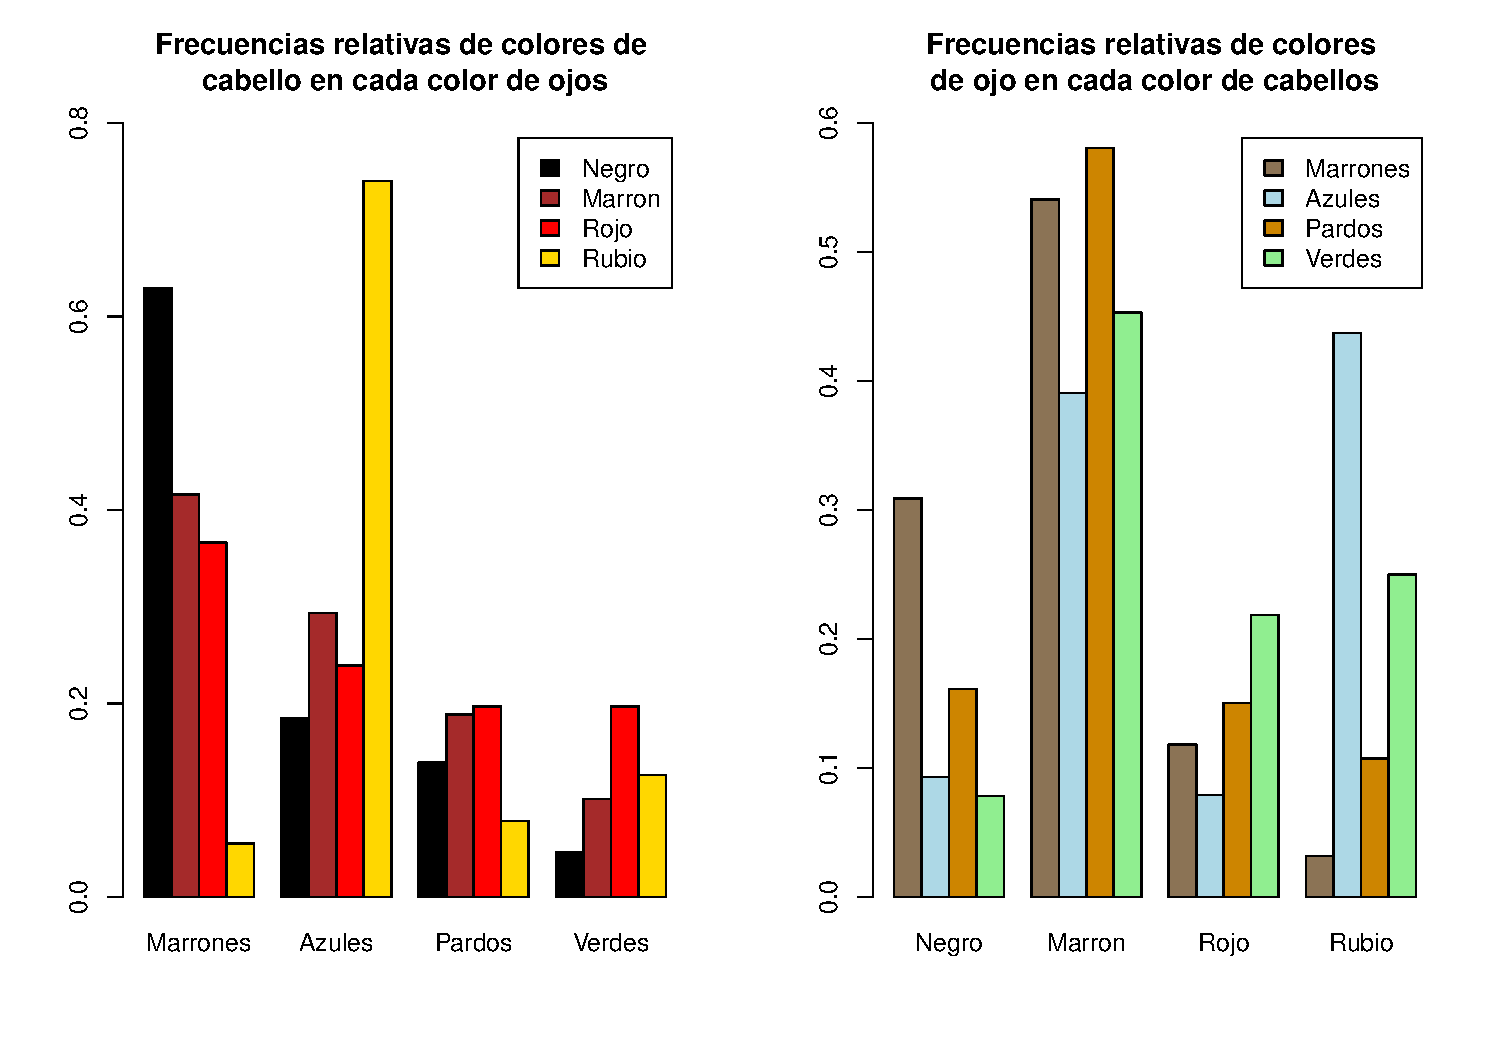
\includegraphics{R_base_files/figure-beamer/unnamed-chunk-107-1.pdf}

Vemos que entre las personas de ojos azules, los cabellos rubios son los
más frecuentes, y que entre las personas castañas el color de ojos más
frecuente es el pardo.
\end{frame}

\begin{frame}[fragile]{Un ejercicio para vosotros}
\phantomsection\label{un-ejercicio-para-vosotros}
\textbf{Ejercicio}

Instalad y cargad el paquete \texttt{MASS}. Encontraréis una tabla de
datos llamada \texttt{birthwt} sobre factores que pueden incidir en el
peso de los niños al nacer. Con \texttt{str()} y \texttt{head()},
explorad la estructura, y con \texttt{help()}, mirad el significado de
cada variable.

\begin{itemize}
\item
  Calculad una tabla de frecuencias relativas marginales de los pares
  (raza de la madre, peso inferior a 2.5 kg o no) que permita ver si la
  raza de la madre influye en el peso del bebé. Dibujad un diagrama de
  mosaico de esta tabla.
\item
  Dibujad un diagrama bidimensional de barras, con las barras
  organizadas en bloques, que permita visualizar esta información. Poned
  nombres adecuados a los bloques, colores a las barras, y añadid una
  leyenda que explique qué representa cada barra. ¿Se puede obtener
  alguna conclusión de esta tabla y de este diagrama de barras?
\item
  Repetid los dos puntos anteriores para los pares (madre fumadora o no,
  peso inferior a 2.5 kg o no) y para los pares (madre hipertensa o no,
  peso inferior a 2.5 kg o no).
\item
  Calculad una tabla de frecuencias relativas marginales de las ternas
  (raza de la madre, madre fumadora o no, peso inferior a 2.5 kg o no)
  que permita ver si la raza de la madre y su condición de fumadora o no
  fumadora influyen en el peso del bebé. Dibujad un diagrama de mosaico
  de esta tabla.
\end{itemize}
\end{frame}

\section{Analisis de datos ordinales}\label{analisis-de-datos-ordinales}

\begin{frame}{Datos ordinales}
\phantomsection\label{datos-ordinales}
Los \# Descripción de datos ordinales
\end{frame}

\begin{frame}{Datos ordinales}
\phantomsection\label{datos-ordinales-1}
Los \blue{datos ordinales} son parecidos a los cualitativos, en el
sentido de que son cualidades de los individuos u objetos.

La diferencia existente entre los datos cualitativos y los ordinales
reside en las características que expresan. En el caso de los ordinales,
éstas tienen un orden natural que permite ``acumular'' observaciones.
\end{frame}

\section{Frecuencias para datos
ordinales}\label{frecuencias-para-datos-ordinales}

\begin{frame}{Frecuencia acumulada}
\phantomsection\label{frecuencia-acumulada}
Al trabajar con datos ordinales, el orden de los niveles de los datos
nos permite calcular no solo frecuencias absolutas y relativas, sino
también \blue{frecuencias acumuladas}.

Es decir, podemos contar cuantas veces hemos observado un dato menor o
igual a este.
\end{frame}

\begin{frame}[fragile]{Ejemplo 1}
\phantomsection\label{ejemplo-1}
\textbf{Ejemplo 1}

Suponed que tenemos una muestra de 15 estudiantes de los cuales sabemos
su nota en el examen de Estadística. Clasificamos todos estos resultados
en Suspenso (\(S\)), Aprobado (\(A\)), Notable (\(N\)) y Excelente
(\(Ex\)) y consideramos su orden natural \(S<A<N<Ex\).

Las notas obtenidas han sido las siguientes
\[S,\ A,\ N,\ Ex,\ S,\ S,\ Ex,\ Ex,\ N,\ A,\ A,\ A,\ A,\ N,\ S\]

Como recordaréis, para saber cuantas hay de cada una (su frecuencia
absoluta), utilizamos la función \texttt{table()}
\end{frame}

\begin{frame}[fragile]{Ejemplo 1}
\phantomsection\label{ejemplo-1-1}
\begin{Shaded}
\begin{Highlighting}[]
\NormalTok{notas }\OtherTok{=} \FunctionTok{ordered}\NormalTok{(}\FunctionTok{c}\NormalTok{(}\StringTok{"S"}\NormalTok{,}\StringTok{"A"}\NormalTok{, }\StringTok{"N"}\NormalTok{, }\StringTok{"Ex"}\NormalTok{, }\StringTok{"S"}\NormalTok{, }\StringTok{"S"}\NormalTok{,}
                  \StringTok{"Ex"}\NormalTok{,}\StringTok{"Ex"}\NormalTok{, }\StringTok{"N"}\NormalTok{, }\StringTok{"A"}\NormalTok{, }\StringTok{"A"}\NormalTok{, }\StringTok{"A"}\NormalTok{,}
                  \StringTok{"A"}\NormalTok{, }\StringTok{"N"}\NormalTok{, }\StringTok{"S"}\NormalTok{),}
                \AttributeTok{levels =} \FunctionTok{c}\NormalTok{(}\StringTok{"S"}\NormalTok{, }\StringTok{"A"}\NormalTok{, }\StringTok{"N"}\NormalTok{, }\StringTok{"Ex"}\NormalTok{))}
\FunctionTok{table}\NormalTok{(notas)}
\end{Highlighting}
\end{Shaded}

\begin{verbatim}
notas
 S  A  N Ex 
 4  5  3  3 
\end{verbatim}

Como podréis observar, hay 4 \(S\), 5 \(A\), 3 \(N\) y 3 \(Ex\).
\end{frame}

\begin{frame}{Ejemplo 1}
\phantomsection\label{ejemplo-1-2}
En lo referente a \textbf{frecuencias absolutas acumuladas}, hay

\begin{itemize}
\tightlist
\item
  4 estudiantes con \(S\) o menos. Ello implica que la frecuencia
  acumulada de \(S\) es 4
\item
  9 estudiantes que han obtenido \(A\) o menos. Entonces, la frecuencia
  acumulada de \(A\) es 9
\item
  12 estudiantes los cuales han obtenido \(N\) o menos. Así, la
  frecuencia acumulada de \(N\) es 12
\item
  15 estudiantes (todos) que han obtenido \(Ex\) o menos. De este modo,
  la frecuencia acumulada de \(Ex\) es 15, o sea, el total.
\end{itemize}
\end{frame}

\begin{frame}{Ejemplo 1}
\phantomsection\label{ejemplo-1-3}
\blue{
Frecuencia relativa acumulada.
} Es la fracción del total de las observaciones en tanto por 1 que
representa su frecuencia absoluta acumulada

Así, las recuencias relativas acumuladas respectivas son

\begin{itemize}
\tightlist
\item
  \(S:\ \frac{4}{15} \approx\) 0.27
\item
  \(A:\ \frac{9}{15}\approx\) 0.6
\item
  \(N:\ \frac{12}{15}\approx\) 0.8
\item
  \(Ex:\ \frac{15}{15}=1\)
\end{itemize}
\end{frame}

\begin{frame}{Frecuencia relativa acumulada}
\phantomsection\label{frecuencia-relativa-acumulada}
En general, supongamos que realizamos \(n\) observaciones

\[x_1,\dots,x_n\]

de un cierto tipo de datos ordinales, cuyos posibles niveles ordenados
son

\[l_1<l_2<\dots<l_k\]

Por tanto, cada una de las observaciones \(x_j\) es igual a algún
\(l_i\). Diremos que todas estas observaciones forman una
\blue{variable ordinal}. En nuestro ejemplo anterior, los 4 niveles eran
\[S<A<N<Ex\]
\end{frame}

\begin{frame}{Frecuencia relativa acumulada}
\phantomsection\label{frecuencia-relativa-acumulada-1}
Además, nuestro \(n = 15\) y nuestros \(x_1,\dots,x_{15}\) son las
calificaciones obtenidas por los alumnos.

De este modo, con estas notaciones

\begin{itemize}
\tightlist
\item
  Las definiciones de frecuencias absolutas \(n_j\) y las relativas
  \(f_j\), para cada nivel \(l_j\) son las mismas que en una variable
  cualitativa.
\item
  Las frecuencia absoluta acumulada del nivel \(l_j\) en esta variable
  ordinal es el número \(N_j\) de observaciones \(x_i\) tales que
  \(x_i\le l_j\). Es decir, \[N_j=\sum_{i=1}^jn_i\]
\end{itemize}
\end{frame}

\begin{frame}{Frecuencia relativa acumulada}
\phantomsection\label{frecuencia-relativa-acumulada-2}
\begin{itemize}
\tightlist
\item
  La frecuencia relativa acumulada del nivel \(l_j\) en esta variable
  ordinal es la fracción en tanto por 1 \(F_j\) de observaciones \(x_i\)
  tales que \(x_i\le l_j\). Es decir,
  \[F_j=\frac{N_j}{n}=\sum_{i=1}^jf_i\]
\end{itemize}
\end{frame}

\begin{frame}[fragile]{Ejemplo 2}
\phantomsection\label{ejemplo-2}
\textbf{Ejemplo 2}

En un estudio, a un grupo de clientes de un restaurante se les hizo la
siguiente pregunta:

``¿Estás contento con el trato ofrecido por los trabajadores del
establecimiento?''

Las posibles respuestas forman una escala ordinal con \(1<2<3<4<5\).

Supongamos que se recogieron las siguientes respuestas de 50 técnicos:

\begin{Shaded}
\begin{Highlighting}[]
\FunctionTok{set.seed}\NormalTok{(}\DecValTok{2018}\NormalTok{)}
\NormalTok{clientes }\OtherTok{=} \FunctionTok{sample}\NormalTok{(}\DecValTok{1}\SpecialCharTok{:}\DecValTok{5}\NormalTok{, }\DecValTok{50}\NormalTok{, }\AttributeTok{replace =} \ConstantTok{TRUE}\NormalTok{)}
\NormalTok{clientes}
\end{Highlighting}
\end{Shaded}

\begin{verbatim}
 [1] 3 4 5 2 5 1 3 4 2 4 3 3 1 1 5 3 1 3 3 5 1 4 2 5 3 4 5 1 2 2 1 5 5 2 1 2 5 5
[39] 2 1 2 1 3 2 1 2 3 3 1 2
\end{verbatim}

\begin{Shaded}
\begin{Highlighting}[]
\FunctionTok{set.seed}\NormalTok{(}\ConstantTok{NULL}\NormalTok{)}
\end{Highlighting}
\end{Shaded}
\end{frame}

\begin{frame}[fragile]{Ejemplo 2}
\phantomsection\label{ejemplo-2-1}
En este caso tenemos 5 niveles (\(k=5\)) y 50 observaciones (\(n=50\))
que forman una variable ordinal a la que hemos llamado
\texttt{clientes}.

Hemos calculado todas sus frecuencias (absoluta, relativa, acumulada y
relativa acumulada) y las hemos representado en la siguiente talbla.

\begin{verbatim}
  Absoluta Relativa Acumulada Rel. Acumulada
1       12     0.24        12           0.24
2       12     0.24        24           0.48
3       11     0.22        35           0.70
4        5     0.10        40           0.80
5       10     0.20        50           1.00
\end{verbatim}

\textbf{Ejercicio.} Calculad todas las frecuencias y comprobad que son
exactamente estas.
\end{frame}

\begin{frame}{Frecuencia relativa acumulada}
\phantomsection\label{frecuencia-relativa-acumulada-3}
Los gráficos para frecuencias absolutas y relativas absolutas de
variables ordinales son exactamente los mismos que para las variables
cualitativas.

También podemos utilizar diagramas de barras para describir frecuencias
acumuladas: en este caso, la altura de cada barra debe ser igual a la
frecuencia acumulada del nivel respectivo. Además, estos niveles deben
de aparecer ordenados de manera ascendente, de forma que las alturas de
las barras también tengan un orden ascendente.

No obstante, se recomienda no hacer uso de diagramas circulares a la
hora de representar frecuencias acumuladas, debido a que éstos no
representan la información sobre la acumulación de datos de forma fácil
de entender a simple vista.
\end{frame}

\section{Descripción de datos ordinales con
R}\label{descripciuxf3n-de-datos-ordinales-con-r}

\begin{frame}[fragile]{Función cumsum()}
\phantomsection\label{funciuxf3n-cumsum}
¿Recordáis la función \texttt{cumsum()}? Pues esta puede ser utilizada a
la hora de calcular frecuencias acumuladas.

Retomemos el ejemplo anterior de las notas de los estudiantes y
calculemos y representemos en un diagrama de barras las frecuencias
acumuladas de la muestra de notas.

\begin{Shaded}
\begin{Highlighting}[]
\NormalTok{notas}
\end{Highlighting}
\end{Shaded}

\begin{verbatim}
 [1] S  A  N  Ex S  S  Ex Ex N  A  A  A  A  N  S 
Levels: S < A < N < Ex
\end{verbatim}

\begin{Shaded}
\begin{Highlighting}[]
\NormalTok{fAbs }\OtherTok{=} \FunctionTok{table}\NormalTok{(notas) }\CommentTok{\#Frec. abs.}
\FunctionTok{cumsum}\NormalTok{(fAbs) }\CommentTok{\#Frec. abs. acumuladas}
\end{Highlighting}
\end{Shaded}

\begin{verbatim}
 S  A  N Ex 
 4  9 12 15 
\end{verbatim}
\end{frame}

\begin{frame}[fragile]{Función cumsum()}
\phantomsection\label{funciuxf3n-cumsum-1}
\begin{Shaded}
\begin{Highlighting}[]
\FunctionTok{cumsum}\NormalTok{(}\FunctionTok{prop.table}\NormalTok{(fAbs)) }\CommentTok{\#Frec. relativas acumuladas}
\end{Highlighting}
\end{Shaded}

\begin{verbatim}
        S         A         N        Ex 
0.2666667 0.6000000 0.8000000 1.0000000 
\end{verbatim}

\begin{Shaded}
\begin{Highlighting}[]
\FunctionTok{barplot}\NormalTok{(fAbs, }\AttributeTok{main =} \StringTok{"Diagrama de barras de}
\StringTok{        frecuencias absolutas"}\NormalTok{)}
\end{Highlighting}
\end{Shaded}

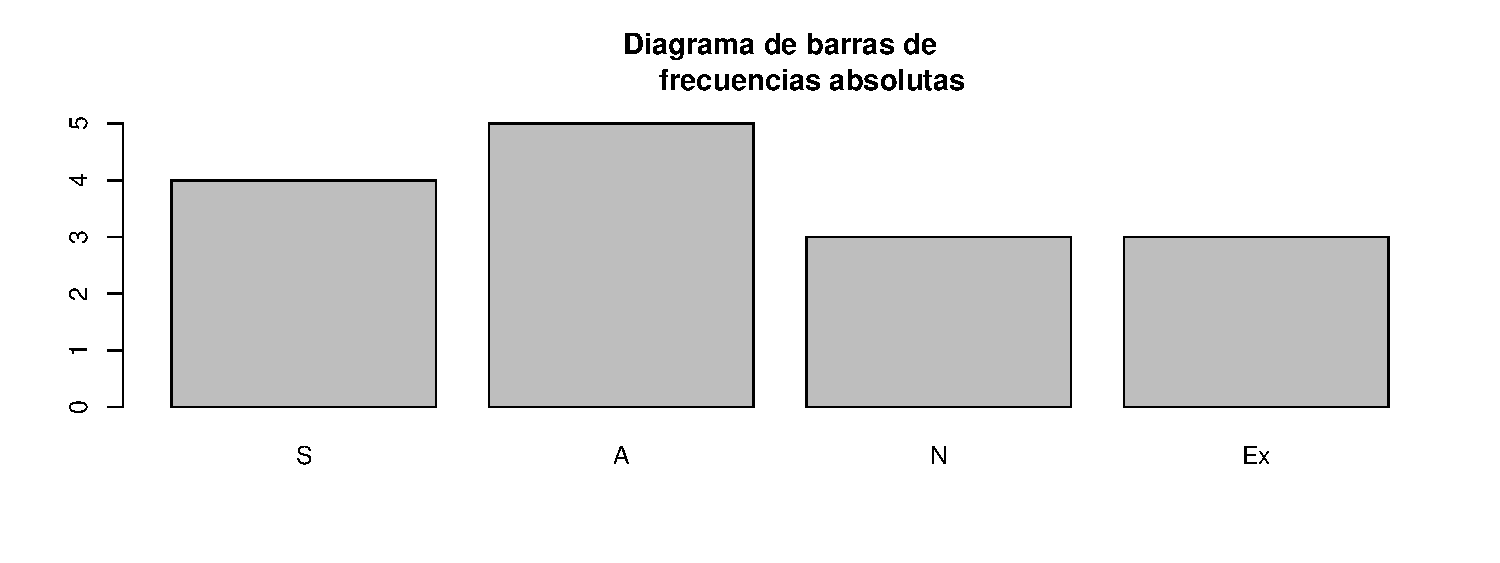
\includegraphics[width=0.8\linewidth]{R_base_files/figure-beamer/unnamed-chunk-112-1}
\end{frame}

\begin{frame}[fragile]{Función cumsum()}
\phantomsection\label{funciuxf3n-cumsum-2}
\begin{Shaded}
\begin{Highlighting}[]
\FunctionTok{barplot}\NormalTok{(}\FunctionTok{cumsum}\NormalTok{(fAbs), }
        \AttributeTok{main =} \StringTok{"Diagrama de barras de }
\StringTok{        frecuencias absolutas acumuladas"}\NormalTok{)}
\end{Highlighting}
\end{Shaded}

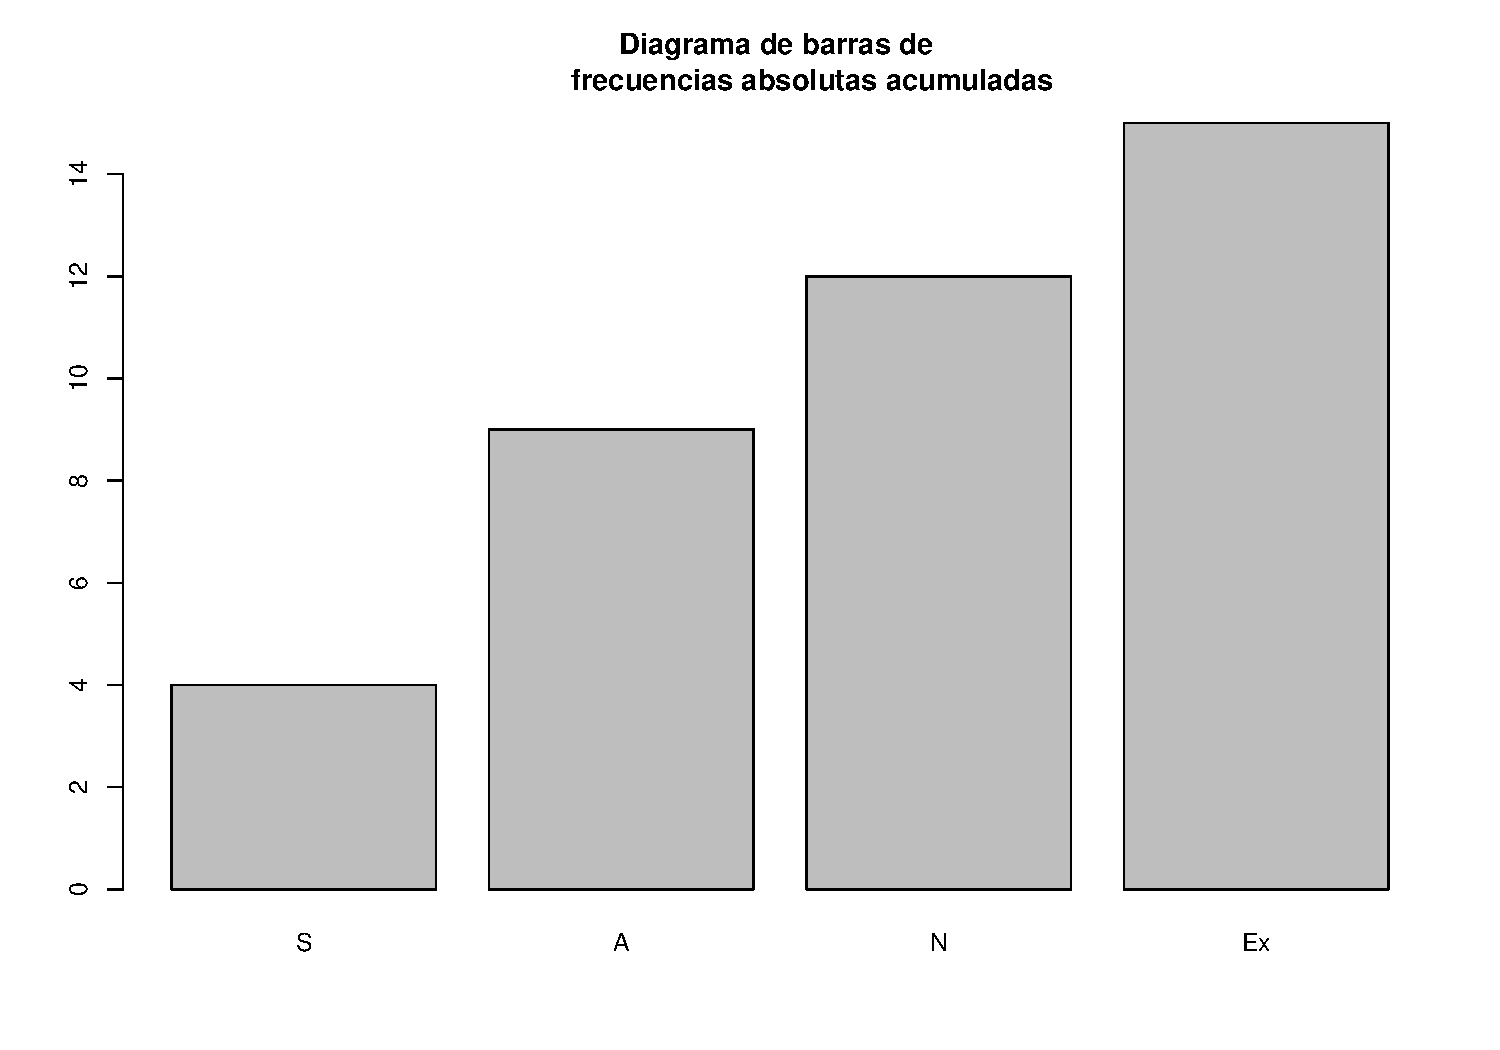
\includegraphics[width=0.8\linewidth]{R_base_files/figure-beamer/unnamed-chunk-113-1}
\end{frame}

\begin{frame}[fragile]{Función cumsum()}
\phantomsection\label{funciuxf3n-cumsum-3}
Podríamos haber calculado las frecuencias relativas acumuladas de la
forma

\begin{Shaded}
\begin{Highlighting}[]
\FunctionTok{cumsum}\NormalTok{(}\FunctionTok{table}\NormalTok{(notas))}\SpecialCharTok{/}\FunctionTok{length}\NormalTok{(notas)}
\end{Highlighting}
\end{Shaded}

\begin{verbatim}
        S         A         N        Ex 
0.2666667 0.6000000 0.8000000 1.0000000 
\end{verbatim}

\begin{Shaded}
\begin{Highlighting}[]
\FunctionTok{cumsum}\NormalTok{(}\FunctionTok{table}\NormalTok{(notas)}\SpecialCharTok{/}\FunctionTok{length}\NormalTok{(notas))}
\end{Highlighting}
\end{Shaded}

\begin{verbatim}
        S         A         N        Ex 
0.2666667 0.6000000 0.8000000 1.0000000 
\end{verbatim}
\end{frame}

\begin{frame}[fragile]{Función cumsum()}
\phantomsection\label{funciuxf3n-cumsum-4}
Pero no podemos hacer \texttt{prop.table(cumsum(table(notas)))}.

\textbf{Ejercicio.} Pensad qué ha entendido R que queríamos hacer con
esta última instrucción.
\end{frame}

\begin{frame}{Ejemplo 3}
\phantomsection\label{ejemplo-3}
\textbf{Ejemplo 3}

Se ha evaluado el tamaño de los cuellos de 100 jirafas. Los niveles que
se han utilizado se los considera ordenados de la siguiente manera:

\[\text{Muy.corto}<\text{Corto}<\text{Normal}<\text{Largo}<\text{Muy.largo}\]

Los valores obtenidos en dicho estudio han sido los siguientes
\end{frame}

\begin{frame}[fragile]{Ejemplo 3}
\phantomsection\label{ejemplo-3-1}
\begin{Shaded}
\begin{Highlighting}[]
\NormalTok{longitud}
\end{Highlighting}
\end{Shaded}

\begin{verbatim}
  [1] Normal    Largo     Muy.largo Corto     Muy.largo Muy.corto Normal   
  [8] Largo     Corto     Largo     Normal    Normal    Muy.corto Muy.corto
 [15] Muy.largo Normal    Muy.corto Normal    Normal    Muy.largo Muy.corto
 [22] Largo     Corto     Muy.largo Normal    Largo     Muy.largo Muy.corto
 [29] Corto     Corto     Muy.corto Muy.largo Muy.largo Corto     Muy.corto
 [36] Corto     Muy.largo Muy.largo Corto     Muy.corto Corto     Muy.corto
 [43] Normal    Corto     Muy.corto Corto     Normal    Normal    Muy.corto
 [50] Corto     Normal    Muy.corto Largo     Largo     Corto     Muy.corto
 [57] Corto     Normal    Normal    Normal    Normal    Muy.corto Normal   
 [64] Muy.corto Corto     Largo     Muy.corto Corto     Muy.corto Muy.largo
 [71] Muy.corto Corto     Muy.largo Largo     Muy.largo Normal    Corto    
 [78] Corto     Normal    Largo     Largo     Corto     Corto     Muy.largo
 [85] Largo     Largo     Normal    Normal    Muy.corto Normal    Corto    
 [92] Normal    Muy.corto Corto     Muy.corto Normal    Corto     Corto    
 [99] Muy.corto Corto    
Levels: Muy.corto < Corto < Normal < Largo < Muy.largo
\end{verbatim}
\end{frame}

\begin{frame}[fragile]{Ejemplo 3}
\phantomsection\label{ejemplo-3-2}
Estudiemos sus frecuencias

\begin{Shaded}
\begin{Highlighting}[]
\NormalTok{Fr.Abs }\OtherTok{=} \FunctionTok{table}\NormalTok{(longitud)}
\NormalTok{Fr.Abs}
\end{Highlighting}
\end{Shaded}

\begin{verbatim}
longitud
Muy.corto     Corto    Normal     Largo Muy.largo 
       23        26        24        13        14 
\end{verbatim}

\begin{Shaded}
\begin{Highlighting}[]
\NormalTok{Fr.Rel }\OtherTok{=} \FunctionTok{prop.table}\NormalTok{(Fr.Abs)}
\NormalTok{Fr.Rel}
\end{Highlighting}
\end{Shaded}

\begin{verbatim}
longitud
Muy.corto     Corto    Normal     Largo Muy.largo 
     0.23      0.26      0.24      0.13      0.14 
\end{verbatim}
\end{frame}

\begin{frame}[fragile]{Ejemplo 3}
\phantomsection\label{ejemplo-3-3}
\begin{Shaded}
\begin{Highlighting}[]
\NormalTok{Fr.Acum }\OtherTok{=} \FunctionTok{cumsum}\NormalTok{(Fr.Abs)}
\NormalTok{Fr.Acum}
\end{Highlighting}
\end{Shaded}

\begin{verbatim}
Muy.corto     Corto    Normal     Largo Muy.largo 
       23        49        73        86       100 
\end{verbatim}

\begin{Shaded}
\begin{Highlighting}[]
\NormalTok{Fr.RAcum }\OtherTok{=} \FunctionTok{cumsum}\NormalTok{(Fr.Rel)}
\NormalTok{Fr.RAcum}
\end{Highlighting}
\end{Shaded}

\begin{verbatim}
Muy.corto     Corto    Normal     Largo Muy.largo 
     0.23      0.49      0.73      0.86      1.00 
\end{verbatim}
\end{frame}

\begin{frame}[fragile]{Ejemplo 3}
\phantomsection\label{ejemplo-3-4}
La instrucción \texttt{barplot} produce el siguiente diagrama de barras
de frecuencias relativas acumuladas

\begin{Shaded}
\begin{Highlighting}[]
\FunctionTok{barplot}\NormalTok{(Fr.RAcum, }\AttributeTok{main =} \StringTok{"Diagrama de frecuencias}
\StringTok{        relativas acumuladas"}\NormalTok{)}
\end{Highlighting}
\end{Shaded}

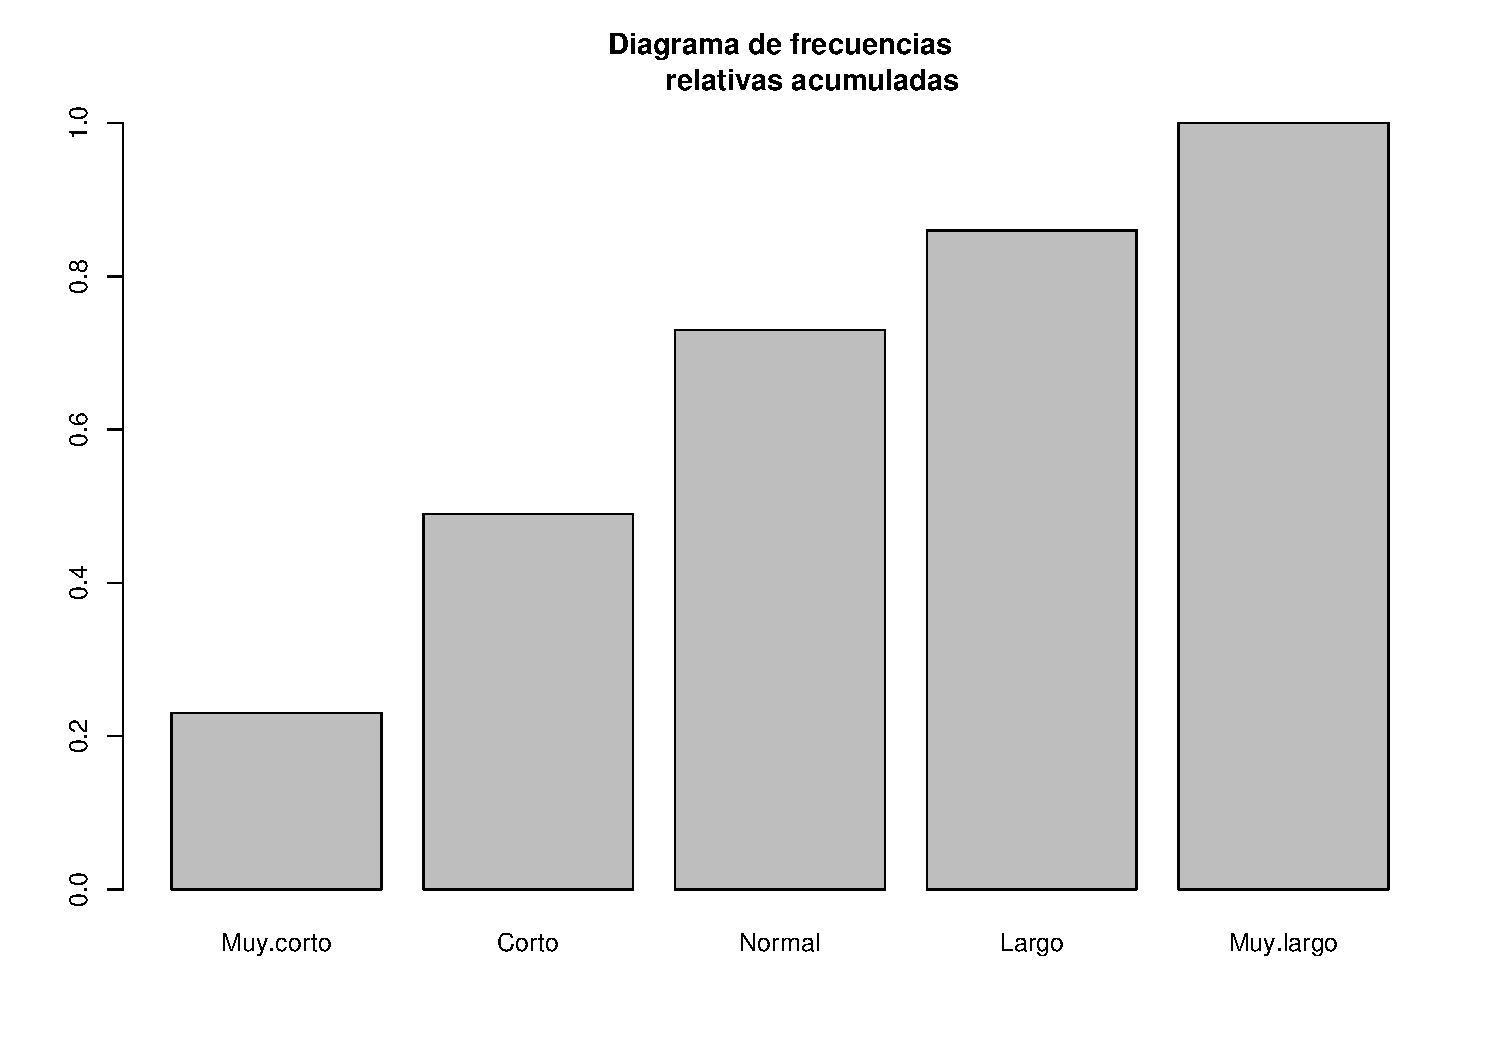
\includegraphics[width=0.6\linewidth]{R_base_files/figure-beamer/unnamed-chunk-120-1}
\end{frame}

\begin{frame}[fragile]{Función cumsum()}
\phantomsection\label{funciuxf3n-cumsum-5}
Para calcular frecuencias acumuladas en una tabla multidimensional, hay
que aplicar a la tabla la función \texttt{cumsum} mediante la función
\texttt{apply} que ya explicábamos para matrices. En este caso en
concreto, la sintaxis de la instrucción sería

\texttt{apply(tabla,\ MARGIN=...,\ FUN=cumsum)}

donde el valor \texttt{MARGIN} ha de ser el de la dimensión en la que
queremos acumular las frecuencias: 1 si queremos hacerlo por filas, 2
para hacerlo por columnas, etc. Lo veremos todo más claro con un ejemplo
\end{frame}

\begin{frame}[fragile]{Ejemplo 4}
\phantomsection\label{ejemplo-4}
\textbf{Ejemplo 4}

Supongamos que en el ejemplo anterior, el de las jirafas, estas
provienen de 4 zonas diferentes, A,B,C y D, de manera que las 30
primeras son de la zona A, las 25 siguientes de la B, las 35 siguientes
de la C y las 10 últimas de la D. Nos interesa estudiar la distribución
de las longitudes según la zona.

Vamos a organizar todos estos datos en un data frame llamado
\texttt{jirafas}. Para que nos sea más fácil visualizar la información,
es conveniente que las filas de las tablas de frecuencias correspondan a
las zonas. Por lo tanto, al definir el data frame, entraremos como
primera variable la de la muestra las zonas. Así, conseguiremos que
éstas aparezcan en las filas al aplicarle la función table.
\end{frame}

\begin{frame}[fragile]{Ejemplo 4}
\phantomsection\label{ejemplo-4-1}
\begin{Shaded}
\begin{Highlighting}[]
\NormalTok{zonas }\OtherTok{=} \FunctionTok{rep}\NormalTok{(}\FunctionTok{c}\NormalTok{(}\StringTok{"A"}\NormalTok{,}\StringTok{"B"}\NormalTok{,}\StringTok{"C"}\NormalTok{,}\StringTok{"D"}\NormalTok{), }\FunctionTok{c}\NormalTok{(}\DecValTok{30}\NormalTok{,}\DecValTok{25}\NormalTok{,}\DecValTok{35}\NormalTok{,}\DecValTok{10}\NormalTok{))}
\NormalTok{jirafas }\OtherTok{=} \FunctionTok{data.frame}\NormalTok{(zonas,longitud)}
\FunctionTok{str}\NormalTok{(jirafas)}
\end{Highlighting}
\end{Shaded}

\begin{verbatim}
'data.frame':   100 obs. of  2 variables:
 $ zonas   : chr  "A" "A" "A" "A" ...
 $ longitud: Ord.factor w/ 5 levels "Muy.corto"<"Corto"<..: 3 4 5 2 5 1 3 4 2 4 ...
\end{verbatim}

\begin{Shaded}
\begin{Highlighting}[]
\FunctionTok{head}\NormalTok{(jirafas)}
\end{Highlighting}
\end{Shaded}

\begin{verbatim}
  zonas  longitud
1     A    Normal
2     A     Largo
3     A Muy.largo
4     A     Corto
5     A Muy.largo
6     A Muy.corto
\end{verbatim}
\end{frame}

\begin{frame}[fragile]{Ejemplo 4}
\phantomsection\label{ejemplo-4-2}
Para calcular la tabla de frecuencias absolutas acumuladas de las
longitudes por zonas y como las zonas definen las filas de la tabla
anterior, debemos utilizar la función \texttt{apply} con
\texttt{MARGIN\ =\ 1}.

\begin{Shaded}
\begin{Highlighting}[]
\FunctionTok{apply}\NormalTok{(}\FunctionTok{table}\NormalTok{(jirafas), }\AttributeTok{MARGIN =} \DecValTok{1}\NormalTok{, }\AttributeTok{FUN =}\NormalTok{ cumsum)}
\end{Highlighting}
\end{Shaded}

\begin{verbatim}
           zonas
longitud     A  B  C  D
  Muy.corto  6  7  7  3
  Corto     11 15 15  8
  Normal    19 19 25 10
  Largo     24 21 31 10
  Muy.largo 30 25 35 10
\end{verbatim}
\end{frame}

\begin{frame}[fragile]{Ejemplo 4}
\phantomsection\label{ejemplo-4-3}
Fijaos que la tabla se ha traspuesto. Resulta que cuando se aplica
\texttt{apply} a una \texttt{table} bidimensional, R intercambia, en
caso de ser necesario, filas por columnas en el resultado para que la
dimensión de la tabla resultante en la que se haya aplicado la función
sea la de las columnas.

Con lo cual, para volver a tener las zonas en las filas, hay que
trasponer el resultado de la función \texttt{apply}.

\begin{Shaded}
\begin{Highlighting}[]
\FunctionTok{t}\NormalTok{(}\FunctionTok{apply}\NormalTok{(}\FunctionTok{table}\NormalTok{(jirafas), }\AttributeTok{MARGIN =} \DecValTok{1}\NormalTok{, }\AttributeTok{FUN =}\NormalTok{ cumsum))}
\end{Highlighting}
\end{Shaded}

\begin{verbatim}
     longitud
zonas Muy.corto Corto Normal Largo Muy.largo
    A         6    11     19    24        30
    B         7    15     19    21        25
    C         7    15     25    31        35
    D         3     8     10    10        10
\end{verbatim}
\end{frame}

\begin{frame}[fragile]{Ejemplo 4}
\phantomsection\label{ejemplo-4-4}
Vamos ahora a calcular la tabla de frecuencias relativas acumuladas de
las longitudes de cuello por zonas. Para conseguirlo, y en una única
instrucción, primero calculamos la tabla de frecuencias relativas por
filas, a continuación, con las funciones \texttt{apply} y
\texttt{cumsum} las acumulamos y, finalmente, trasponemos el resultado.

\begin{Shaded}
\begin{Highlighting}[]
\FunctionTok{t}\NormalTok{(}\FunctionTok{apply}\NormalTok{(}\FunctionTok{prop.table}\NormalTok{(}\FunctionTok{table}\NormalTok{(jirafas),}
                   \AttributeTok{margin =} \DecValTok{1}\NormalTok{), }
        \AttributeTok{MARGIN =} \DecValTok{1}\NormalTok{, }\AttributeTok{FUN =}\NormalTok{ cumsum))}
\end{Highlighting}
\end{Shaded}

\begin{verbatim}
     longitud
zonas Muy.corto     Corto    Normal     Largo Muy.largo
    A      0.20 0.3666667 0.6333333 0.8000000         1
    B      0.28 0.6000000 0.7600000 0.8400000         1
    C      0.20 0.4285714 0.7142857 0.8857143         1
    D      0.30 0.8000000 1.0000000 1.0000000         1
\end{verbatim}
\end{frame}

\begin{frame}[fragile]{Ejemplo 4}
\phantomsection\label{ejemplo-4-5}
Vamos ahora a dibujar el diagrama de barras por bloques de esta tabla.
Nos interesa que las barras de este diagrama se agrupen por zonas.
Entonces, tendremos que aplicar \texttt{barplot} a la tabla sin
trasponer.

Además, vamos a colocar la leyenda en la esquina superior izquierda para
que no se superponga a ninguna barra. También reduciremos el tamaño del
texto de la leyenda para que quepa completamente.
\end{frame}

\begin{frame}[fragile]{Ejemplo 4}
\phantomsection\label{ejemplo-4-6}
\begin{Shaded}
\begin{Highlighting}[]
\NormalTok{Diagrama }\OtherTok{=} \FunctionTok{apply}\NormalTok{(}\FunctionTok{prop.table}\NormalTok{(}\FunctionTok{table}\NormalTok{(jirafas), }\AttributeTok{margin =} \DecValTok{1}\NormalTok{),}
                 \AttributeTok{MARGIN =} \DecValTok{1}\NormalTok{, }\AttributeTok{FUN =}\NormalTok{ cumsum)}
\FunctionTok{barplot}\NormalTok{(Diagrama, }\AttributeTok{beside =} \ConstantTok{TRUE}\NormalTok{, }\AttributeTok{legend =} \ConstantTok{TRUE}\NormalTok{,}
\AttributeTok{main =} \StringTok{"Diagrama de barras de }
\StringTok{        frecuencias relativas acumuladas }
\StringTok{        de longitudes por zonas"}\NormalTok{,}
\AttributeTok{args.legend=}\FunctionTok{list}\NormalTok{(}\AttributeTok{x=}\StringTok{"topleft"}\NormalTok{, }\AttributeTok{cex=}\FloatTok{0.55}\NormalTok{))}
\end{Highlighting}
\end{Shaded}

\begin{center}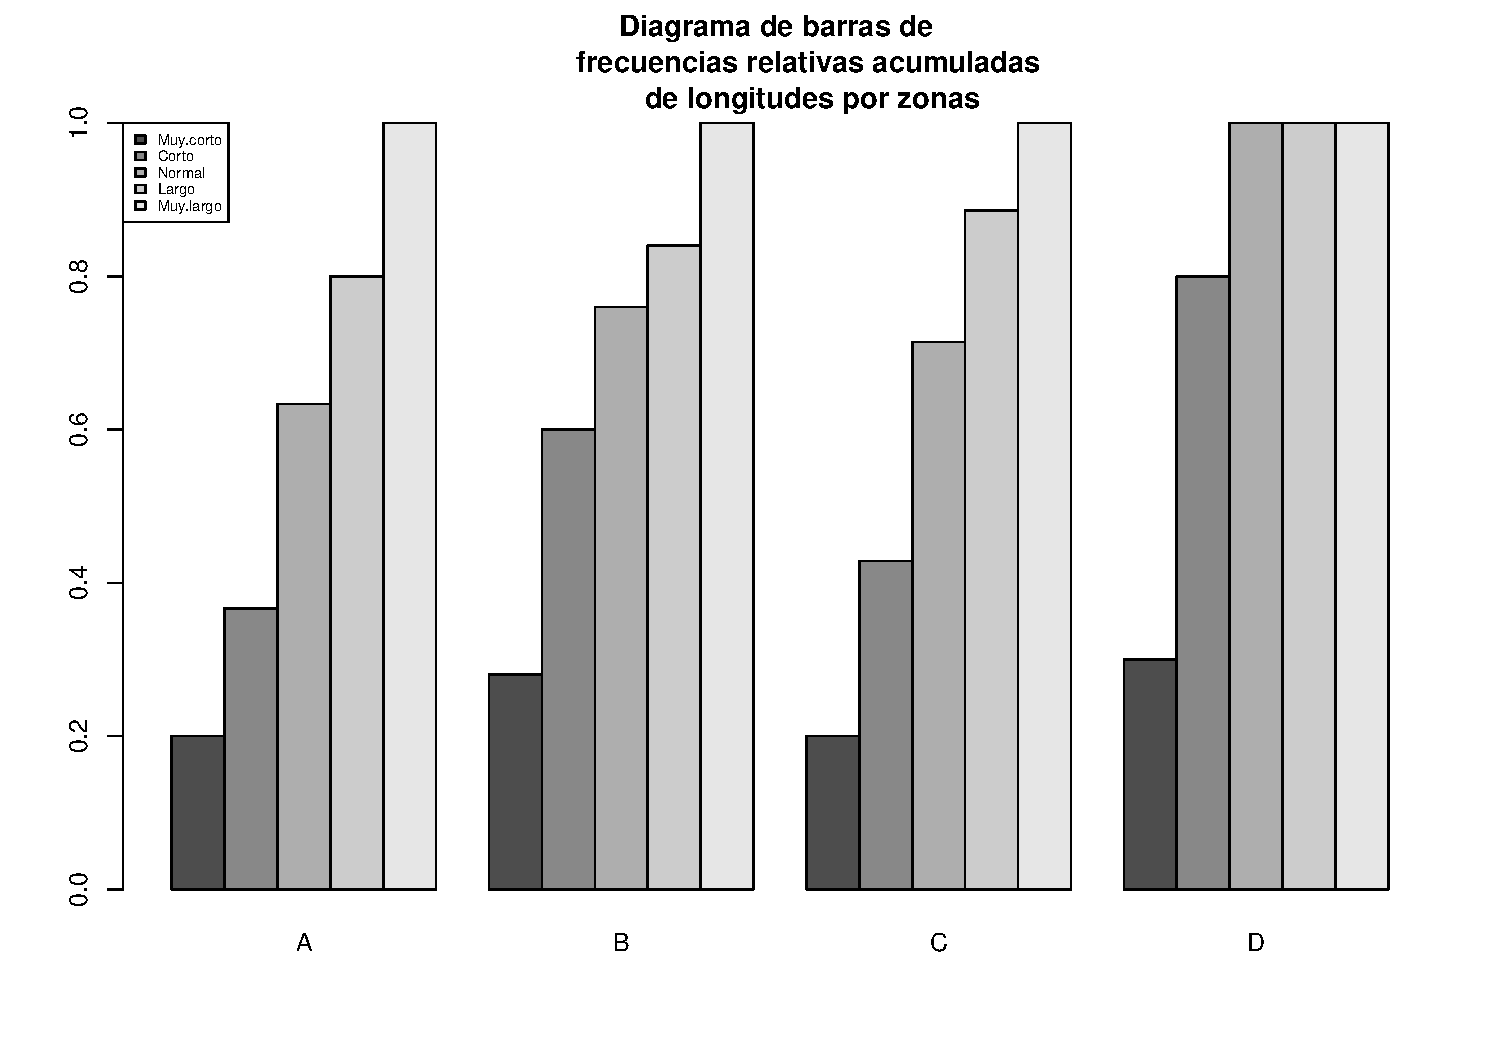
\includegraphics[width=0.5\linewidth]{R_base_files/figure-beamer/unnamed-chunk-125-1} \end{center}
\end{frame}

\begin{frame}[fragile]{Ejemplo 5}
\phantomsection\label{ejemplo-5}
\textbf{Ejemplo 5}

Consideremos el data frame \texttt{datacrab} y arreglemos los datos.

\begin{Shaded}
\begin{Highlighting}[]
\NormalTok{crabs }\OtherTok{=} \FunctionTok{read.table}\NormalTok{(}\StringTok{"../data/datacrab.txt"}\NormalTok{, }\AttributeTok{header =} \ConstantTok{TRUE}\NormalTok{)}
\NormalTok{crabs }\OtherTok{=}\NormalTok{ crabs[,}\SpecialCharTok{{-}}\DecValTok{1}\NormalTok{] }\CommentTok{\#Omitimos la primera columna}
\FunctionTok{str}\NormalTok{(crabs)}
\end{Highlighting}
\end{Shaded}

\begin{verbatim}
'data.frame':   173 obs. of  5 variables:
 $ color : int  3 4 2 4 4 3 2 4 3 4 ...
 $ spine : int  3 3 1 3 3 3 1 2 1 3 ...
 $ width : num  28.3 22.5 26 24.8 26 23.8 26.5 24.7 23.7 25.6 ...
 $ satell: int  8 0 9 0 4 0 0 0 0 0 ...
 $ weight: int  3050 1550 2300 2100 2600 2100 2350 1900 1950 2150 ...
\end{verbatim}

La variable numérica \texttt{width} contiene la anchura de cada cangrejo
\end{frame}

\begin{frame}[fragile]{Ejemplo 5}
\phantomsection\label{ejemplo-5-1}
\begin{Shaded}
\begin{Highlighting}[]
\FunctionTok{table}\NormalTok{(crabs}\SpecialCharTok{$}\NormalTok{width)}
\end{Highlighting}
\end{Shaded}

\begin{verbatim}

  21   22 22.5 22.9   23 23.1 23.2 23.4 23.5 23.7 23.8 23.9   24 24.1 24.2 24.3 
   1    1    3    3    2    3    1    1    1    3    3    1    2    1    2    2 
24.5 24.7 24.8 24.9   25 25.1 25.2 25.3 25.4 25.5 25.6 25.7 25.8 25.9   26 26.1 
   7    5    1    3    6    2    2    1    3    3    2    6    7    1    6    2 
26.2 26.3 26.5 26.7 26.8   27 27.1 27.2 27.3 27.4 27.5 27.6 27.7 27.8 27.9   28 
   8    1    6    3    3    5    2    2    1    3    6    1    2    2    2    3 
28.2 28.3 28.4 28.5 28.7 28.9   29 29.3 29.5 29.7 29.8   30 30.2 30.3 30.5 31.7 
   4    3    2    4    2    1    6    2    1    1    1    3    1    1    1    1 
31.9 33.5 
   1    1 
\end{verbatim}
\end{frame}

\begin{frame}[fragile]{Ejemplo 5}
\phantomsection\label{ejemplo-5-2}
Vamos a convertir a la variable \texttt{width} en una variable ordinal
que agrupe las entradas de la variable original en niveles.

La manera más sencilla de llevarlo a cabo es utilizando la función
\texttt{cut}, que estudiaremos en detalle en lecciones posteriores. Por
ahora, basta con saber que la instrucción dividirá el vector numérico
\texttt{crabs\$width} en intervalos de extremos los puntos especificados
en el argumento \texttt{breaks}. El parámetro \texttt{right\ =\ FALSE}
sirve para indicar que los puntos de corte pertenecen la intervalo de su
derecha, e \texttt{Inf} indica \(\infty\).

Por lo tanto, nosotros llevaremos a cabo la siguiente instrucción

\begin{Shaded}
\begin{Highlighting}[]
\NormalTok{intervalos }\OtherTok{=} \FunctionTok{cut}\NormalTok{(crabs}\SpecialCharTok{$}\NormalTok{width, }\AttributeTok{breaks =} \FunctionTok{c}\NormalTok{(}\DecValTok{21}\NormalTok{,}\DecValTok{25}\NormalTok{,}\DecValTok{29}\NormalTok{,}\DecValTok{33}\NormalTok{,}\ConstantTok{Inf}\NormalTok{), }\AttributeTok{right =} \ConstantTok{FALSE}\NormalTok{, }
                 \AttributeTok{labels =} \FunctionTok{c}\NormalTok{(}\StringTok{"21{-}25"}\NormalTok{, }\StringTok{"25{-}29"}\NormalTok{, }\StringTok{"29{-}33"}\NormalTok{, }\StringTok{"33{-}..."}\NormalTok{))}
\end{Highlighting}
\end{Shaded}
\end{frame}

\begin{frame}[fragile]{Ejemplo 5}
\phantomsection\label{ejemplo-5-3}
El resultado de la instrucción es un factor que tiene como niveles estos
intervalos, identificados con las etiquetas especificadas en el
parámetro \texttt{labels}. Como nostros vamos a usar estos intervalos
como niveles de una variable ordinal, además convertiremos este factor
en ordenado.

\begin{Shaded}
\begin{Highlighting}[]
\NormalTok{crabs}\SpecialCharTok{$}\NormalTok{width.rank }\OtherTok{=} \FunctionTok{ordered}\NormalTok{(intervalos)}
\FunctionTok{str}\NormalTok{(crabs)}
\end{Highlighting}
\end{Shaded}

\begin{verbatim}
'data.frame':   173 obs. of  6 variables:
 $ color     : int  3 4 2 4 4 3 2 4 3 4 ...
 $ spine     : int  3 3 1 3 3 3 1 2 1 3 ...
 $ width     : num  28.3 22.5 26 24.8 26 23.8 26.5 24.7 23.7 25.6 ...
 $ satell    : int  8 0 9 0 4 0 0 0 0 0 ...
 $ weight    : int  3050 1550 2300 2100 2600 2100 2350 1900 1950 2150 ...
 $ width.rank: Ord.factor w/ 4 levels "21-25"<"25-29"<..: 2 1 2 1 2 1 2 1 1 2 ...
\end{verbatim}
\end{frame}

\begin{frame}[fragile]{Ejemplo 5}
\phantomsection\label{ejemplo-5-4}
Nos interesa estudiar la distribución de las anchuras de los cangrejos
según el número de colores. Por lo tanto, vamos a calcular las tablas
bidimensionales de frecuencais relativas y relativas acumuladas de los
intervalos de las anchuras en cada nivel de \texttt{color} y las
representaremos por medio de diagramas de barras.

La tabla de frecuencias absolutas de los pares se puede obtener
aplicando \texttt{table} al data frame formado por la primera y última
columnas.

\begin{Shaded}
\begin{Highlighting}[]
\NormalTok{Tabla }\OtherTok{=} \FunctionTok{table}\NormalTok{(crabs[,}\FunctionTok{c}\NormalTok{(}\DecValTok{1}\NormalTok{,}\DecValTok{6}\NormalTok{)])}
\NormalTok{Tabla}
\end{Highlighting}
\end{Shaded}

\begin{verbatim}
     width.rank
color 21-25 25-29 29-33 33-...
    2     1     9     2      0
    3    19    62    13      1
    4    17    24     3      0
    5     9    12     1      0
\end{verbatim}
\end{frame}

\begin{frame}[fragile]{Ejemplo 5}
\phantomsection\label{ejemplo-5-5}
\begin{Shaded}
\begin{Highlighting}[]
\NormalTok{Fr.rel }\OtherTok{=} \FunctionTok{round}\NormalTok{(}\FunctionTok{prop.table}\NormalTok{(Tabla,}\AttributeTok{margin =} \DecValTok{1}\NormalTok{),}\DecValTok{3}\NormalTok{)}
\NormalTok{Fr.rel}
\end{Highlighting}
\end{Shaded}

\begin{verbatim}
     width.rank
color 21-25 25-29 29-33 33-...
    2 0.083 0.750 0.167  0.000
    3 0.200 0.653 0.137  0.011
    4 0.386 0.545 0.068  0.000
    5 0.409 0.545 0.045  0.000
\end{verbatim}
\end{frame}

\begin{frame}[fragile]{Ejemplo 5}
\phantomsection\label{ejemplo-5-6}
\begin{Shaded}
\begin{Highlighting}[]
\NormalTok{Fr.rel.acu }\OtherTok{=} \FunctionTok{round}\NormalTok{(}\FunctionTok{apply}\NormalTok{(}\FunctionTok{prop.table}\NormalTok{(Tabla, }\AttributeTok{margin =} \DecValTok{1}\NormalTok{), }\AttributeTok{MARGIN =} \DecValTok{1}\NormalTok{, }\AttributeTok{FUN =}\NormalTok{ cumsum), }\DecValTok{3}\NormalTok{)}
\FunctionTok{t}\NormalTok{(Fr.rel.acu)}
\end{Highlighting}
\end{Shaded}

\begin{verbatim}
     width.rank
color 21-25 25-29 29-33 33-...
    2 0.083 0.833 1.000      1
    3 0.200 0.853 0.989      1
    4 0.386 0.932 1.000      1
    5 0.409 0.955 1.000      1
\end{verbatim}
\end{frame}

\begin{frame}[fragile]{Ejemplo 5}
\phantomsection\label{ejemplo-5-7}
\begin{Shaded}
\begin{Highlighting}[]
\NormalTok{azul }\OtherTok{=} \FunctionTok{c}\NormalTok{(}\StringTok{"cyan"}\NormalTok{, }\StringTok{"cyan4"}\NormalTok{, }\StringTok{"cyan1"}\NormalTok{, }\StringTok{"cyan3"}\NormalTok{)}

\FunctionTok{barplot}\NormalTok{(}\FunctionTok{t}\NormalTok{(Fr.rel), }\AttributeTok{beside =} \ConstantTok{TRUE}\NormalTok{, }\AttributeTok{legend =} \ConstantTok{TRUE}\NormalTok{, }\AttributeTok{ylim =} \FunctionTok{c}\NormalTok{(}\DecValTok{0}\NormalTok{,}\DecValTok{1}\NormalTok{), }\AttributeTok{col =}\NormalTok{ azul, }
        \AttributeTok{main =} \StringTok{"Diagrama de barras de frecuencias relativas"}\NormalTok{, }
        \AttributeTok{args.legend=}\FunctionTok{list}\NormalTok{(}\AttributeTok{x =} \StringTok{"topright"}\NormalTok{, }\AttributeTok{cex=}\FloatTok{0.55}\NormalTok{))}
\end{Highlighting}
\end{Shaded}

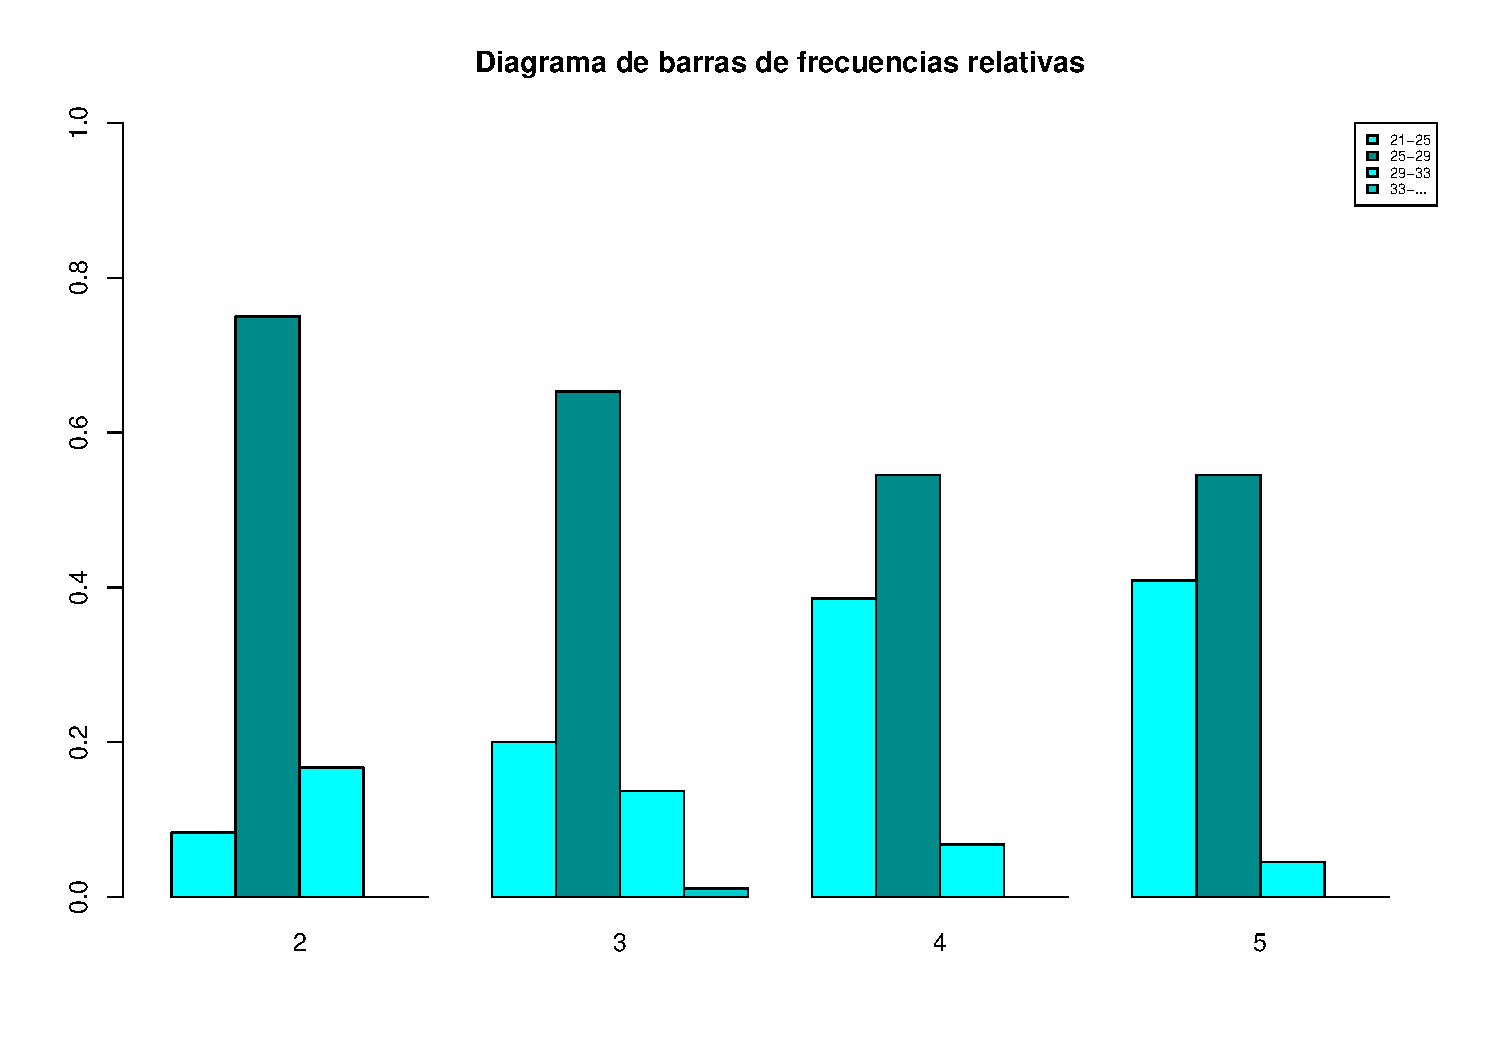
\includegraphics[width=0.8\linewidth]{R_base_files/figure-beamer/unnamed-chunk-133-1}
\end{frame}

\begin{frame}[fragile]{Ejemplo 5}
\phantomsection\label{ejemplo-5-8}
\begin{Shaded}
\begin{Highlighting}[]
\FunctionTok{barplot}\NormalTok{(Fr.rel.acu, }\AttributeTok{beside =} \ConstantTok{TRUE}\NormalTok{, }\AttributeTok{legend =} \ConstantTok{TRUE}\NormalTok{, }\AttributeTok{col =}\NormalTok{ azul, }
        \AttributeTok{main =} \StringTok{"Diagrama de barras de frecuencias relativas acumuladas"}\NormalTok{, }
        \AttributeTok{args.legend=}\FunctionTok{list}\NormalTok{(}\AttributeTok{x =} \StringTok{"topleft"}\NormalTok{, }\AttributeTok{cex=}\FloatTok{0.55}\NormalTok{))}
\end{Highlighting}
\end{Shaded}

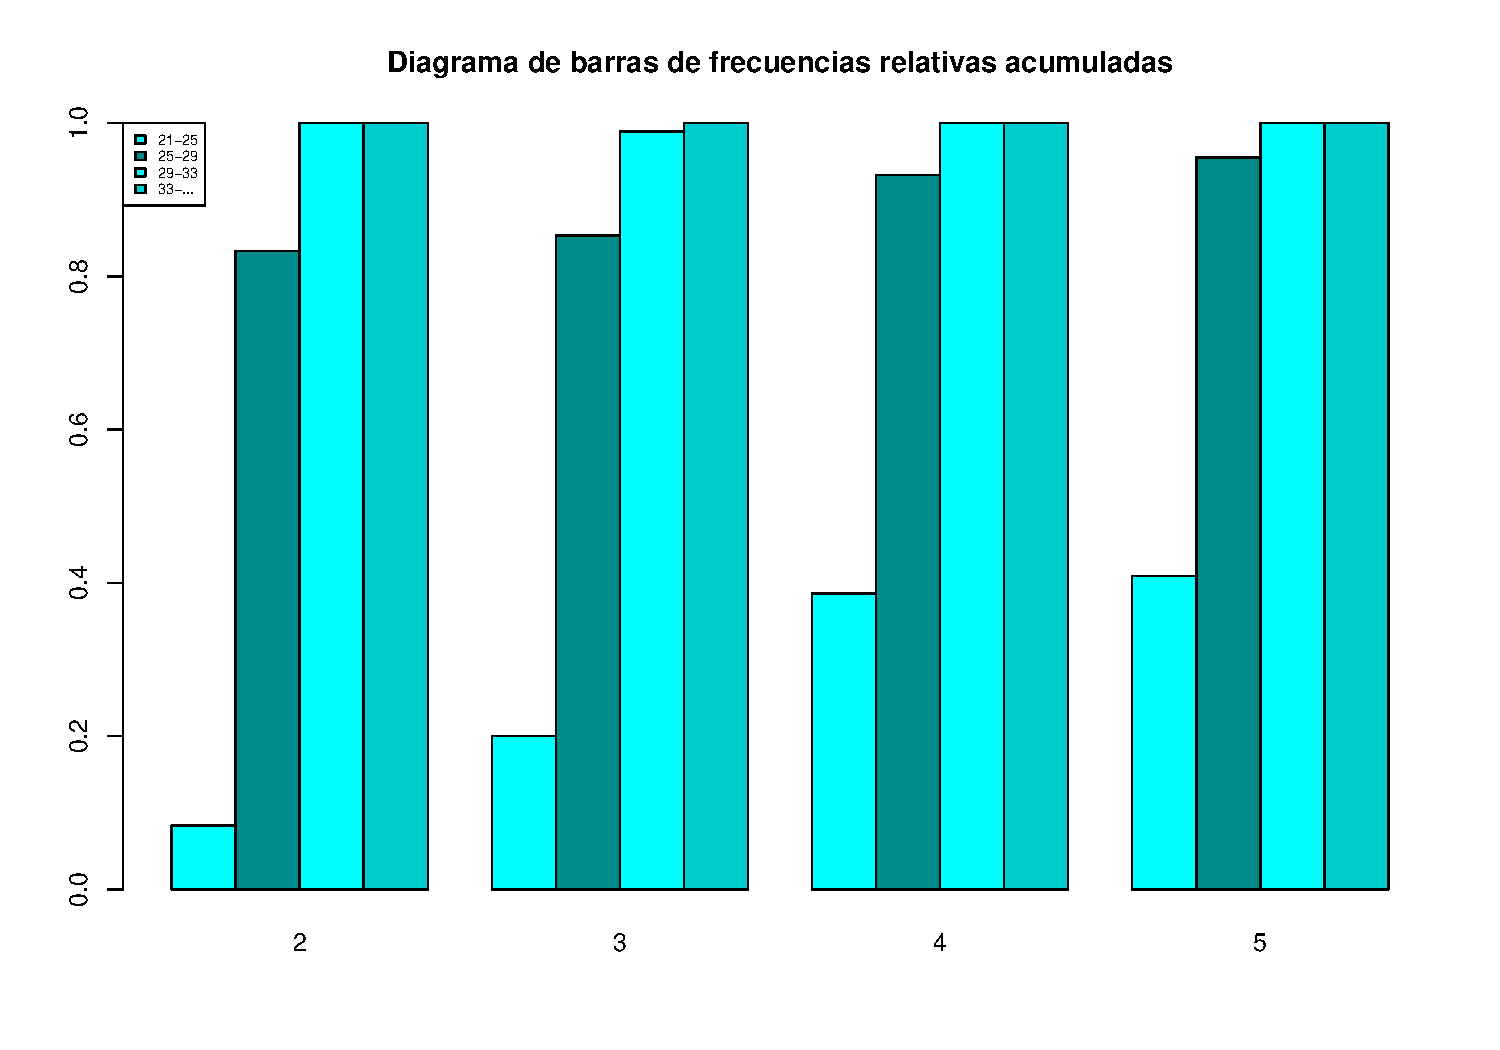
\includegraphics[width=0.8\linewidth]{R_base_files/figure-beamer/unnamed-chunk-134-1}

Los \blue{datos ordinales} son parecidos a los cualitativos, en el
sentido de que son cualidades de los individuos u objetos.

La diferencia existente entre los datos cualitativos y los ordinales
reside en las características que expresan. En el caso de los ordinales,
éstas tienen un orden natural que permite ``acumular'' observaciones.
\end{frame}

\section{Frecuencias para datos
ordinales}\label{frecuencias-para-datos-ordinales-1}

\begin{frame}{Frecuencia acumulada}
\phantomsection\label{frecuencia-acumulada-1}
Al trabajar con datos ordinales, el orden de los niveles de los datos
nos permite calcular no solo frecuencias absolutas y relativas, sino
también \blue{frecuencias acumuladas}.

Es decir, podemos contar cuantas veces hemos observado un dato menor o
igual a este.
\end{frame}

\begin{frame}[fragile]{Ejemplo 1}
\phantomsection\label{ejemplo-1-4}
\textbf{Ejemplo 1}

Suponed que tenemos una muestra de 15 estudiantes de los cuales sabemos
su nota en el examen de Estadística. Clasificamos todos estos resultados
en Suspenso (\(S\)), Aprobado (\(A\)), Notable (\(N\)) y Excelente
(\(Ex\)) y consideramos su orden natural \(S<A<N<Ex\).

Las notas obtenidas han sido las siguientes
\[S,\ A,\ N,\ Ex,\ S,\ S,\ Ex,\ Ex,\ N,\ A,\ A,\ A,\ A,\ N,\ S\]

Como recordaréis, para saber cuantas hay de cada una (su frecuencia
absoluta), utilizamos la función \texttt{table()}
\end{frame}

\begin{frame}[fragile]{Ejemplo 1}
\phantomsection\label{ejemplo-1-5}
\begin{Shaded}
\begin{Highlighting}[]
\NormalTok{notas }\OtherTok{=} \FunctionTok{ordered}\NormalTok{(}\FunctionTok{c}\NormalTok{(}\StringTok{"S"}\NormalTok{,}\StringTok{"A"}\NormalTok{, }\StringTok{"N"}\NormalTok{, }\StringTok{"Ex"}\NormalTok{, }\StringTok{"S"}\NormalTok{, }\StringTok{"S"}\NormalTok{, }\StringTok{"Ex"}\NormalTok{, }\StringTok{"Ex"}\NormalTok{, }\StringTok{"N"}\NormalTok{, }\StringTok{"A"}\NormalTok{, }\StringTok{"A"}\NormalTok{, }\StringTok{"A"}\NormalTok{,}
                  \StringTok{"A"}\NormalTok{, }\StringTok{"N"}\NormalTok{, }\StringTok{"S"}\NormalTok{), }\AttributeTok{levels =} \FunctionTok{c}\NormalTok{(}\StringTok{"S"}\NormalTok{, }\StringTok{"A"}\NormalTok{, }\StringTok{"N"}\NormalTok{, }\StringTok{"Ex"}\NormalTok{))}
\FunctionTok{table}\NormalTok{(notas)}
\end{Highlighting}
\end{Shaded}

\begin{verbatim}
notas
 S  A  N Ex 
 4  5  3  3 
\end{verbatim}

Como podréis observar, hay 4 \(S\), 5 \(A\), 3 \(N\) y 3 \(Ex\).
\end{frame}

\begin{frame}{Ejemplo 1}
\phantomsection\label{ejemplo-1-6}
En lo referente a \textbf{frecuencias absolutas acumuladas}, hay

\begin{itemize}
\tightlist
\item
  4 estudiantes con \(S\) o menos. Ello implica que la frecuencia
  acumulada de \(S\) es 4
\item
  9 estudiantes que han obtenido \(A\) o menos. Entonces, la frecuencia
  acumulada de \(A\) es 9
\item
  12 estudiantes los cuales han obtenido \(N\) o menos. Así, la
  frecuencia acumulada de \(N\) es 12
\item
  15 estudiantes (todos) que han obtenido \(Ex\) o menos. De este modo,
  la frecuencia acumulada de \(Ex\) es 15, o sea, el total.
\end{itemize}
\end{frame}

\begin{frame}{Ejemplo 1}
\phantomsection\label{ejemplo-1-7}
\blue{
Frecuencia relativa acumulada.
} Es la fracción del total de las observaciones en tanto por 1 que
representa su frecuencia absoluta acumulada

Así, las recuencias relativas acumuladas respectivas son

\begin{itemize}
\tightlist
\item
  \(S:\ \frac{4}{15} \approx\) 0.27
\item
  \(A:\ \frac{9}{15}\approx\) 0.6
\item
  \(N:\ \frac{12}{15}\approx\) 0.8
\item
  \(Ex:\ \frac{15}{15}=1\)
\end{itemize}
\end{frame}

\begin{frame}{Frecuencia relativa acumulada}
\phantomsection\label{frecuencia-relativa-acumulada-4}
En general, supongamos que realizamos \(n\) observaciones

\[x_1,\dots,x_n\]

de un cierto tipo de datos ordinales, cuyos posibles niveles ordenados
son

\[l_1<l_2<\dots<l_k\]

Por tanto, cada una de las observaciones \(x_j\) es igual a algún
\(l_i\). Diremos que todas estas observaciones forman una
\blue{variable ordinal}. En nuestro ejemplo anterior, los 4 niveles eran
\[S<A<N<Ex\]
\end{frame}

\begin{frame}{Frecuencia relativa acumulada}
\phantomsection\label{frecuencia-relativa-acumulada-5}
Además, nuestro \(n = 15\) y nuestros \(x_1,\dots,x_{15}\) son las
calificaciones obtenidas por los alumnos.

De este modo, con estas notaciones

\begin{itemize}
\tightlist
\item
  Las definiciones de frecuencias absolutas \(n_j\) y las relativas
  \(f_j\), para cada nivel \(l_j\) son las mismas que en una variable
  cualitativa.
\item
  Las frecuencia absoluta acumulada del nivel \(l_j\) en esta variable
  ordinal es el número \(N_j\) de observaciones \(x_i\) tales que
  \(x_i\le l_j\). Es decir, \[N_j=\sum_{i=1}^jn_i\]
\end{itemize}
\end{frame}

\begin{frame}{Frecuencia relativa acumulada}
\phantomsection\label{frecuencia-relativa-acumulada-6}
\begin{itemize}
\tightlist
\item
  La frecuencia relativa acumulada del nivel \(l_j\) en esta variable
  ordinal es la fracción en tanto por 1 \(F_j\) de observaciones \(x_i\)
  tales que \(x_i\le l_j\). Es decir,
  \[F_j=\frac{N_j}{n}=\sum_{i=1}^jf_i\]
\end{itemize}
\end{frame}

\begin{frame}[fragile]{Ejemplo 2}
\phantomsection\label{ejemplo-2-2}
\textbf{Ejemplo 2}

En un estudio, a un grupo de clientes de un restaurante se les hizo la
siguiente pregunta:

``¿Estás contento con el trato ofrecido por los trabajadores del
establecimiento?''

Las posibles respuestas forman una escala ordinal con \(1<2<3<4<5\).

Supongamos que se recogieron las siguientes respuestas de 50 técnicos:

\begin{Shaded}
\begin{Highlighting}[]
\FunctionTok{set.seed}\NormalTok{(}\DecValTok{2018}\NormalTok{)}
\NormalTok{clientes }\OtherTok{=} \FunctionTok{sample}\NormalTok{(}\DecValTok{1}\SpecialCharTok{:}\DecValTok{5}\NormalTok{, }\DecValTok{50}\NormalTok{, }\AttributeTok{replace =} \ConstantTok{TRUE}\NormalTok{)}
\NormalTok{clientes}
\end{Highlighting}
\end{Shaded}

\begin{verbatim}
 [1] 3 4 5 2 5 1 3 4 2 4 3 3 1 1 5 3 1 3 3 5 1 4 2 5 3 4 5 1 2 2 1 5 5 2 1 2 5 5
[39] 2 1 2 1 3 2 1 2 3 3 1 2
\end{verbatim}

\begin{Shaded}
\begin{Highlighting}[]
\FunctionTok{set.seed}\NormalTok{(}\ConstantTok{NULL}\NormalTok{)}
\end{Highlighting}
\end{Shaded}
\end{frame}

\begin{frame}[fragile]{Ejemplo 2}
\phantomsection\label{ejemplo-2-3}
En este caso tenemos 5 niveles (\(k=5\)) y 50 observaciones (\(n=50\))
que forman una variable ordinal a la que hemos llamado
\texttt{clientes}.

Hemos calculado todas sus frecuencias (absoluta, relativa, acumulada y
relativa acumulada) y las hemos representado en la siguiente talbla.

\begin{verbatim}
  Absoluta Relativa Acumulada Rel. Acumulada
1       12     0.24        12           0.24
2       12     0.24        24           0.48
3       11     0.22        35           0.70
4        5     0.10        40           0.80
5       10     0.20        50           1.00
\end{verbatim}

\textbf{Ejercicio.} Calculad todas las frecuencias y comprobad que son
exactamente estas.
\end{frame}

\begin{frame}{Frecuencia relativa acumulada}
\phantomsection\label{frecuencia-relativa-acumulada-7}
Los gráficos para frecuencias absolutas y relativas absolutas de
variables ordinales son exactamente los mismos que para las variables
cualitativas.

También podemos utilizar diagramas de barras para describir frecuencias
acumuladas: en este caso, la altura de cada barra debe ser igual a la
frecuencia acumulada del nivel respectivo. Además, estos niveles deben
de aparecer ordenados de manera ascendente, de forma que las alturas de
las barras también tengan un orden ascendente.

No obstante, se recomienda no hacer uso de diagramas circulares a la
hora de representar frecuencias acumuladas, debido a que éstos no
representan la información sobre la acumulación de datos de forma fácil
de entender a simple vista.
\end{frame}

\section{Descripción de datos ordinales con
R}\label{descripciuxf3n-de-datos-ordinales-con-r-1}

\begin{frame}[fragile]{Función cumsum()}
\phantomsection\label{funciuxf3n-cumsum-6}
¿Recordáis la función \texttt{cumsum()}? Pues esta puede ser utilizada a
la hora de calcular frecuencias acumuladas.

Retomemos el ejemplo anterior de las notas de los estudiantes y
calculemos y representemos en un diagrama de barras las frecuencias
acumuladas de la muestra de notas.

\begin{Shaded}
\begin{Highlighting}[]
\NormalTok{notas}
\end{Highlighting}
\end{Shaded}

\begin{verbatim}
 [1] S  A  N  Ex S  S  Ex Ex N  A  A  A  A  N  S 
Levels: S < A < N < Ex
\end{verbatim}

\begin{Shaded}
\begin{Highlighting}[]
\NormalTok{fAbs }\OtherTok{=} \FunctionTok{table}\NormalTok{(notas) }\CommentTok{\#Frec. abs.}
\FunctionTok{cumsum}\NormalTok{(fAbs) }\CommentTok{\#Frec. abs. acumuladas}
\end{Highlighting}
\end{Shaded}

\begin{verbatim}
 S  A  N Ex 
 4  9 12 15 
\end{verbatim}
\end{frame}

\begin{frame}[fragile]{Función cumsum()}
\phantomsection\label{funciuxf3n-cumsum-7}
\begin{Shaded}
\begin{Highlighting}[]
\FunctionTok{cumsum}\NormalTok{(}\FunctionTok{prop.table}\NormalTok{(fAbs)) }\CommentTok{\#Frec. relativas acumuladas}
\end{Highlighting}
\end{Shaded}

\begin{verbatim}
        S         A         N        Ex 
0.2666667 0.6000000 0.8000000 1.0000000 
\end{verbatim}

\begin{Shaded}
\begin{Highlighting}[]
\FunctionTok{barplot}\NormalTok{(fAbs, }
        \AttributeTok{main =} \StringTok{"Diagrama de barras de frecuencias absolutas"}\NormalTok{)}
\end{Highlighting}
\end{Shaded}

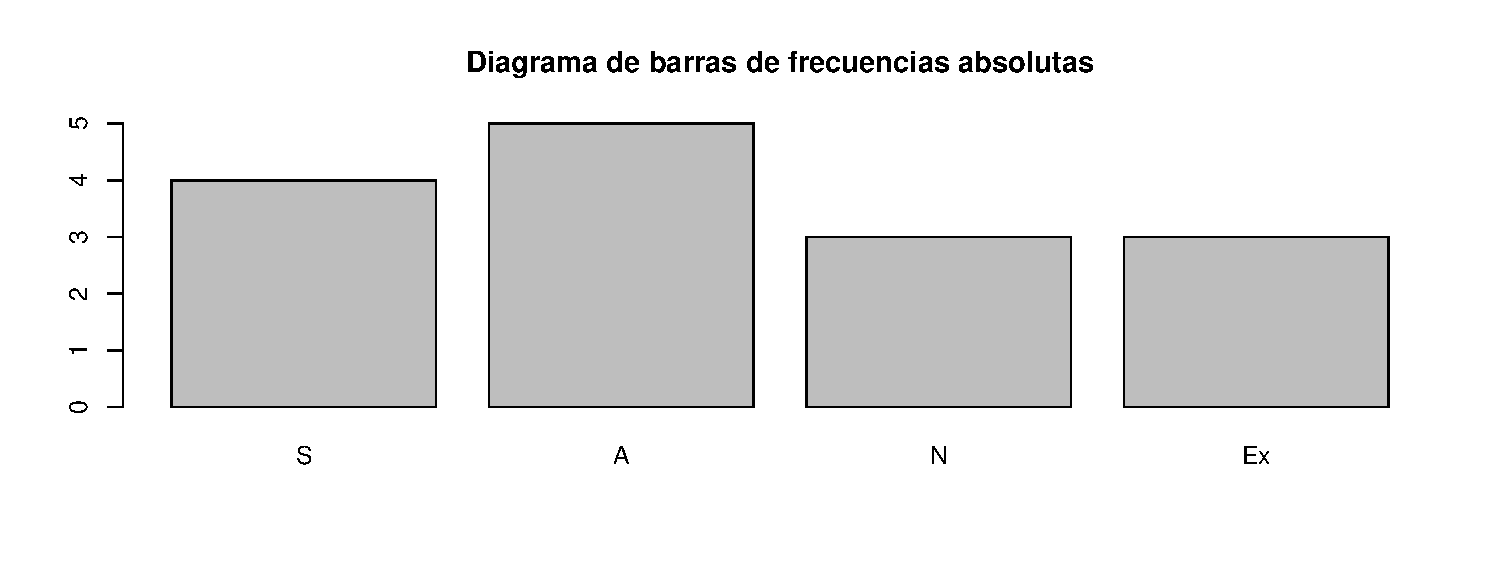
\includegraphics[width=0.8\linewidth]{R_base_files/figure-beamer/unnamed-chunk-139-1}
\end{frame}

\begin{frame}[fragile]{Función cumsum()}
\phantomsection\label{funciuxf3n-cumsum-8}
\begin{Shaded}
\begin{Highlighting}[]
\FunctionTok{barplot}\NormalTok{(}\FunctionTok{cumsum}\NormalTok{(fAbs), }
        \AttributeTok{main =} \StringTok{"Diagrama de barras de frecuencias}
\StringTok{        absolutas acumuladas"}\NormalTok{)}
\end{Highlighting}
\end{Shaded}

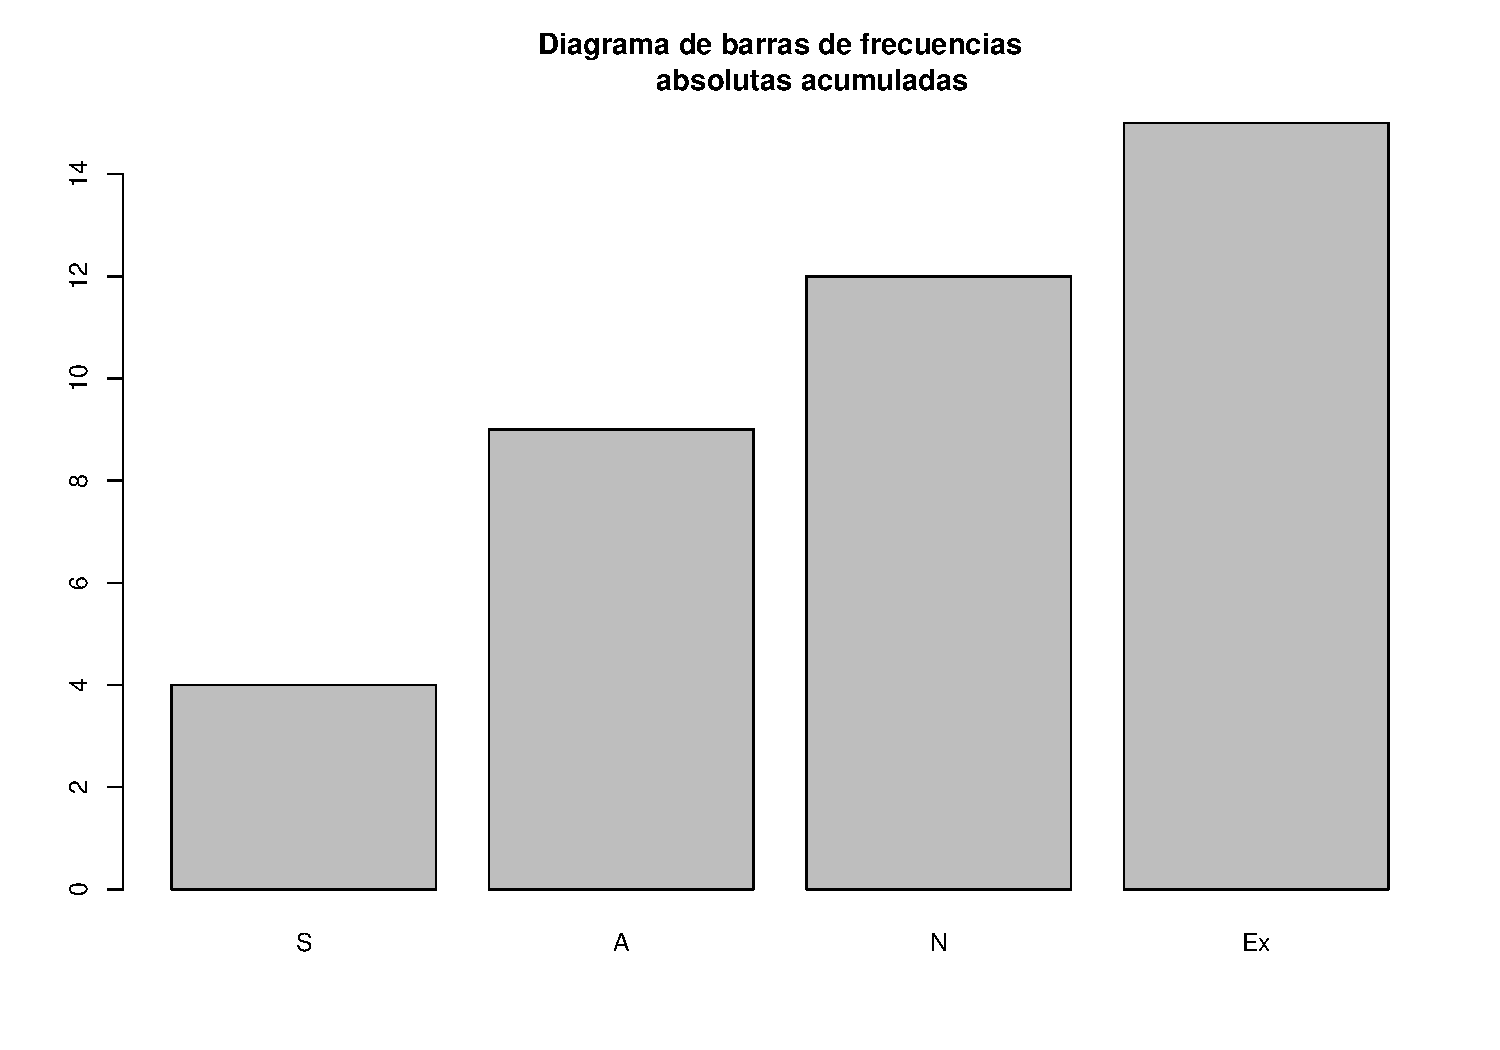
\includegraphics[width=0.5\linewidth]{R_base_files/figure-beamer/unnamed-chunk-140-1}
\end{frame}

\begin{frame}[fragile]{Función cumsum()}
\phantomsection\label{funciuxf3n-cumsum-9}
Podríamos haber calculado las frecuencias relativas acumuladas de la
forma

\begin{Shaded}
\begin{Highlighting}[]
\FunctionTok{cumsum}\NormalTok{(}\FunctionTok{table}\NormalTok{(notas))}\SpecialCharTok{/}\FunctionTok{length}\NormalTok{(notas)}
\end{Highlighting}
\end{Shaded}

\begin{verbatim}
        S         A         N        Ex 
0.2666667 0.6000000 0.8000000 1.0000000 
\end{verbatim}

\begin{Shaded}
\begin{Highlighting}[]
\FunctionTok{cumsum}\NormalTok{(}\FunctionTok{table}\NormalTok{(notas)}\SpecialCharTok{/}\FunctionTok{length}\NormalTok{(notas))}
\end{Highlighting}
\end{Shaded}

\begin{verbatim}
        S         A         N        Ex 
0.2666667 0.6000000 0.8000000 1.0000000 
\end{verbatim}
\end{frame}

\begin{frame}[fragile]{Función cumsum()}
\phantomsection\label{funciuxf3n-cumsum-10}
Pero no podemos hacer \texttt{prop.table(cumsum(table(notas)))}.

\textbf{Ejercicio.} Pensad qué ha entendido R que queríamos hacer con
esta última instrucción.
\end{frame}

\begin{frame}{Ejemplo 3}
\phantomsection\label{ejemplo-3-5}
\textbf{Ejemplo 3}

Se ha evaluado el tamaño de los cuellos de 100 jirafas. Los niveles que
se han utilizado se los considera ordenados de la siguiente manera:

\[\text{Muy.corto}<\text{Corto}<\text{Normal}<\text{Largo}<\text{Muy.largo}\]

Los valores obtenidos en dicho estudio han sido los siguientes
\end{frame}

\begin{frame}[fragile]{Ejemplo 3}
\phantomsection\label{ejemplo-3-6}
\begin{Shaded}
\begin{Highlighting}[]
\NormalTok{longitud}
\end{Highlighting}
\end{Shaded}

\begin{verbatim}
  [1] Normal    Largo     Muy.largo Corto     Muy.largo Muy.corto Normal   
  [8] Largo     Corto     Largo     Normal    Normal    Muy.corto Muy.corto
 [15] Muy.largo Normal    Muy.corto Normal    Normal    Muy.largo Muy.corto
 [22] Largo     Corto     Muy.largo Normal    Largo     Muy.largo Muy.corto
 [29] Corto     Corto     Muy.corto Muy.largo Muy.largo Corto     Muy.corto
 [36] Corto     Muy.largo Muy.largo Corto     Muy.corto Corto     Muy.corto
 [43] Normal    Corto     Muy.corto Corto     Normal    Normal    Muy.corto
 [50] Corto     Normal    Muy.corto Largo     Largo     Corto     Muy.corto
 [57] Corto     Normal    Normal    Normal    Normal    Muy.corto Normal   
 [64] Muy.corto Corto     Largo     Muy.corto Corto     Muy.corto Muy.largo
 [71] Muy.corto Corto     Muy.largo Largo     Muy.largo Normal    Corto    
 [78] Corto     Normal    Largo     Largo     Corto     Corto     Muy.largo
 [85] Largo     Largo     Normal    Normal    Muy.corto Normal    Corto    
 [92] Normal    Muy.corto Corto     Muy.corto Normal    Corto     Corto    
 [99] Muy.corto Corto    
Levels: Muy.corto < Corto < Normal < Largo < Muy.largo
\end{verbatim}
\end{frame}

\begin{frame}[fragile]{Ejemplo 3}
\phantomsection\label{ejemplo-3-7}
Estudiemos sus frecuencias

\begin{Shaded}
\begin{Highlighting}[]
\NormalTok{Fr.Abs }\OtherTok{=} \FunctionTok{table}\NormalTok{(longitud)}
\NormalTok{Fr.Abs}
\end{Highlighting}
\end{Shaded}

\begin{verbatim}
longitud
Muy.corto     Corto    Normal     Largo Muy.largo 
       23        26        24        13        14 
\end{verbatim}

\begin{Shaded}
\begin{Highlighting}[]
\NormalTok{Fr.Rel }\OtherTok{=} \FunctionTok{prop.table}\NormalTok{(Fr.Abs)}
\NormalTok{Fr.Rel}
\end{Highlighting}
\end{Shaded}

\begin{verbatim}
longitud
Muy.corto     Corto    Normal     Largo Muy.largo 
     0.23      0.26      0.24      0.13      0.14 
\end{verbatim}
\end{frame}

\begin{frame}[fragile]{Ejemplo 3}
\phantomsection\label{ejemplo-3-8}
\begin{Shaded}
\begin{Highlighting}[]
\NormalTok{Fr.Acum }\OtherTok{=} \FunctionTok{cumsum}\NormalTok{(Fr.Abs)}
\NormalTok{Fr.Acum}
\end{Highlighting}
\end{Shaded}

\begin{verbatim}
Muy.corto     Corto    Normal     Largo Muy.largo 
       23        49        73        86       100 
\end{verbatim}

\begin{Shaded}
\begin{Highlighting}[]
\NormalTok{Fr.RAcum }\OtherTok{=} \FunctionTok{cumsum}\NormalTok{(Fr.Rel)}
\NormalTok{Fr.RAcum}
\end{Highlighting}
\end{Shaded}

\begin{verbatim}
Muy.corto     Corto    Normal     Largo Muy.largo 
     0.23      0.49      0.73      0.86      1.00 
\end{verbatim}
\end{frame}

\begin{frame}[fragile]{Ejemplo 3}
\phantomsection\label{ejemplo-3-9}
La instrucción \texttt{barplot} produce el siguiente diagrama de barras
de frecuencias relativas acumuladas

\begin{Shaded}
\begin{Highlighting}[]
\FunctionTok{barplot}\NormalTok{(Fr.RAcum, }\AttributeTok{main =} \StringTok{"Diagrama de frecuencias}
\StringTok{        relativas acumuladas"}\NormalTok{)}
\end{Highlighting}
\end{Shaded}

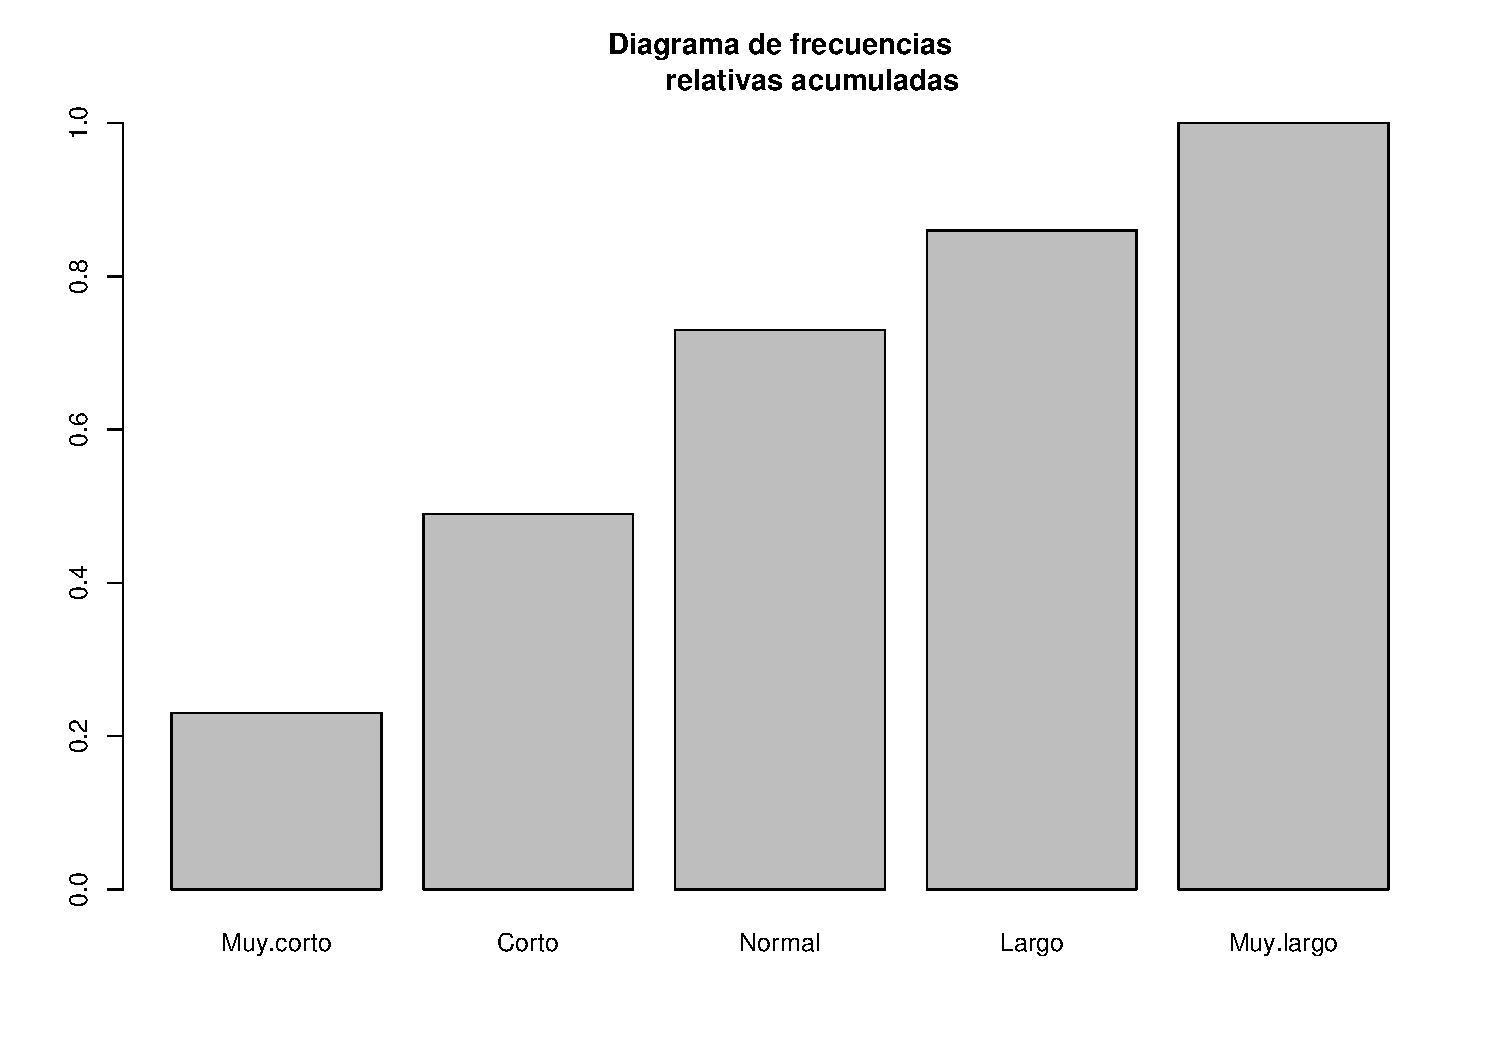
\includegraphics[width=0.7\linewidth]{R_base_files/figure-beamer/unnamed-chunk-147-1}
\end{frame}

\begin{frame}[fragile]{Función cumsum()}
\phantomsection\label{funciuxf3n-cumsum-11}
Para calcular frecuencias acumuladas en una tabla multidimensional, hay
que aplicar a la tabla la función \texttt{cumsum} mediante la función
\texttt{apply} que ya explicábamos para matrices. En este caso en
concreto, la sintaxis de la instrucción es

\texttt{apply(tabla,\ MARGIN=...,\ FUN=cumsum)}

donde el valor \texttt{MARGIN} ha de ser el de la dimensión en la que
queremos acumular las frecuencias: 1 si queremos hacerlo por filas, 2
para hacerlo por columnas, etc. Lo veremos todo más claro con un ejemplo
\end{frame}

\begin{frame}[fragile]{Ejemplo 4}
\phantomsection\label{ejemplo-4-7}
\textbf{Ejemplo 4}

Supongamos que en el ejemplo anterior, el de las jirafas, estas
provienen de 4 zonas diferentes, A,B,C y D, de manera que las 30
primeras son de la zona A, las 25 siguientes de la B, las 35 siguientes
de la C y las 10 últimas de la D. Nos interesa estudiar la distribución
de las longitudes según la zona.

Vamos a organizar todos estos datos en un data frame llamado
\texttt{jirafas}. Para que nos sea más fácil visualizar la información,
es conveniente que las filas de las tablas de frecuencias correspondan a
las zonas. Por lo tanto, al definir el data frame, entraremos como
primera variable la de la muestra las zonas. Así, conseguiremos que
éstas aparezcan en las filas al aplicarle la función table.
\end{frame}

\begin{frame}[fragile]{Ejemplo 4}
\phantomsection\label{ejemplo-4-8}
\begin{Shaded}
\begin{Highlighting}[]
\NormalTok{zonas }\OtherTok{=} \FunctionTok{rep}\NormalTok{(}\FunctionTok{c}\NormalTok{(}\StringTok{"A"}\NormalTok{,}\StringTok{"B"}\NormalTok{,}\StringTok{"C"}\NormalTok{,}\StringTok{"D"}\NormalTok{), }\FunctionTok{c}\NormalTok{(}\DecValTok{30}\NormalTok{,}\DecValTok{25}\NormalTok{,}\DecValTok{35}\NormalTok{,}\DecValTok{10}\NormalTok{))}
\NormalTok{jirafas }\OtherTok{=} \FunctionTok{data.frame}\NormalTok{(zonas,longitud)}
\FunctionTok{str}\NormalTok{(jirafas)}
\end{Highlighting}
\end{Shaded}

\begin{verbatim}
'data.frame':   100 obs. of  2 variables:
 $ zonas   : chr  "A" "A" "A" "A" ...
 $ longitud: Ord.factor w/ 5 levels "Muy.corto"<"Corto"<..: 3 4 5 2 5 1 3 4 2 4 ...
\end{verbatim}

\begin{Shaded}
\begin{Highlighting}[]
\FunctionTok{head}\NormalTok{(jirafas)}
\end{Highlighting}
\end{Shaded}

\begin{verbatim}
  zonas  longitud
1     A    Normal
2     A     Largo
3     A Muy.largo
4     A     Corto
5     A Muy.largo
6     A Muy.corto
\end{verbatim}
\end{frame}

\begin{frame}[fragile]{Ejemplo 4}
\phantomsection\label{ejemplo-4-9}
Para calcular la tabla de frecuencias absolutas acumuladas de las
longitudes por zonas y como las zonas definen las filas de la tabla
anterior, debemos utilizar la función \texttt{apply} con
\texttt{MARGIN\ =\ 1}.

\begin{Shaded}
\begin{Highlighting}[]
\FunctionTok{apply}\NormalTok{(}\FunctionTok{table}\NormalTok{(jirafas), }\AttributeTok{MARGIN =} \DecValTok{1}\NormalTok{, }\AttributeTok{FUN =}\NormalTok{ cumsum)}
\end{Highlighting}
\end{Shaded}

\begin{verbatim}
           zonas
longitud     A  B  C  D
  Muy.corto  6  7  7  3
  Corto     11 15 15  8
  Normal    19 19 25 10
  Largo     24 21 31 10
  Muy.largo 30 25 35 10
\end{verbatim}
\end{frame}

\begin{frame}[fragile]{Ejemplo 4}
\phantomsection\label{ejemplo-4-10}
Fijaos que la tabla se ha traspuesto. Resulta que cuando se aplica
\texttt{apply} a una \texttt{table} bidimensional, R intercambia, en
caso de ser necesario, filas por columnas en el resultado para que la
dimensión de la tabla resultante en la que se haya aplicado la función
sea la de las columnas.

Con lo cual, para volver a tener las zonas en las filas, hay que
trasponer el resultado de la función \texttt{apply}.

\begin{Shaded}
\begin{Highlighting}[]
\FunctionTok{t}\NormalTok{(}\FunctionTok{apply}\NormalTok{(}\FunctionTok{table}\NormalTok{(jirafas), }\AttributeTok{MARGIN =} \DecValTok{1}\NormalTok{, }\AttributeTok{FUN =}\NormalTok{ cumsum))}
\end{Highlighting}
\end{Shaded}

\begin{verbatim}
     longitud
zonas Muy.corto Corto Normal Largo Muy.largo
    A         6    11     19    24        30
    B         7    15     19    21        25
    C         7    15     25    31        35
    D         3     8     10    10        10
\end{verbatim}
\end{frame}

\begin{frame}[fragile]{Ejemplo 4}
\phantomsection\label{ejemplo-4-11}
Vamos ahora a calcular la tabla de frecuencias relativas acumuladas de
las longitudes de cuello por zonas. Para conseguirlo, y en una única
instrucción, primero calculamos la tabla de frecuencias relativas por
filas, a continuación, con las funciones \texttt{apply} y
\texttt{cumsum} las acumulamos y, finalmente, trasponemos el resultado.

\begin{Shaded}
\begin{Highlighting}[]
\FunctionTok{t}\NormalTok{(}\FunctionTok{apply}\NormalTok{(}\FunctionTok{prop.table}\NormalTok{(}\FunctionTok{table}\NormalTok{(jirafas), }\AttributeTok{margin =} \DecValTok{1}\NormalTok{), }\AttributeTok{MARGIN =} \DecValTok{1}\NormalTok{, }\AttributeTok{FUN =}\NormalTok{ cumsum))}
\end{Highlighting}
\end{Shaded}

\begin{verbatim}
     longitud
zonas Muy.corto     Corto    Normal     Largo Muy.largo
    A      0.20 0.3666667 0.6333333 0.8000000         1
    B      0.28 0.6000000 0.7600000 0.8400000         1
    C      0.20 0.4285714 0.7142857 0.8857143         1
    D      0.30 0.8000000 1.0000000 1.0000000         1
\end{verbatim}
\end{frame}

\begin{frame}[fragile]{Ejemplo 4}
\phantomsection\label{ejemplo-4-12}
Vamos ahora a dibujar el diagrama de barras por bloques de esta tabla.
Nos interesa que las barras de este diagrama se agrupen por zonas.
Entonces, tendremos que aplicar \texttt{barplot} a la tabla sin
trasponer.

Además, vamos a colocar la leyenda en la esquina superior izquierda para
que no se superponga a ninguna barra. También reduciremos el tamaño del
texto de la leyenda para que quepa completamente.
\end{frame}

\begin{frame}[fragile]{Ejemplo 4}
\phantomsection\label{ejemplo-4-13}
\begin{Shaded}
\begin{Highlighting}[]
\NormalTok{Diagrama }\OtherTok{=} \FunctionTok{apply}\NormalTok{(}\FunctionTok{prop.table}\NormalTok{(}\FunctionTok{table}\NormalTok{(jirafas), }\AttributeTok{margin =} \DecValTok{1}\NormalTok{), }\AttributeTok{MARGIN =} \DecValTok{1}\NormalTok{, }\AttributeTok{FUN =}\NormalTok{ cumsum)}
\FunctionTok{barplot}\NormalTok{(Diagrama, }\AttributeTok{beside =} \ConstantTok{TRUE}\NormalTok{, }\AttributeTok{legend =} \ConstantTok{TRUE}\NormalTok{, }\AttributeTok{main =} \StringTok{"Diagrama de barras de }
\StringTok{        frecuencias relativas acumuladas de longitudes por zonas"}\NormalTok{,}
\AttributeTok{args.legend=}\FunctionTok{list}\NormalTok{(}\AttributeTok{x=}\StringTok{"topleft"}\NormalTok{, }\AttributeTok{cex=}\FloatTok{0.55}\NormalTok{))}
\end{Highlighting}
\end{Shaded}

\includegraphics[width=0.8\linewidth]{R_base_files/figure-beamer/unnamed-chunk-152-1}
\end{frame}

\begin{frame}[fragile]{Ejemplo 5}
\phantomsection\label{ejemplo-5-9}
\textbf{Ejemplo 5}

Consideremos el data frame \texttt{datacrab} y arreglemos los datos.

\begin{Shaded}
\begin{Highlighting}[]
\NormalTok{crabs }\OtherTok{=} \FunctionTok{read.table}\NormalTok{(}\StringTok{"../data/datacrab.txt"}\NormalTok{, }\AttributeTok{header =} \ConstantTok{TRUE}\NormalTok{)}
\NormalTok{crabs }\OtherTok{=}\NormalTok{ crabs[,}\SpecialCharTok{{-}}\DecValTok{1}\NormalTok{] }\CommentTok{\#Omitimos la primera columna}
\FunctionTok{str}\NormalTok{(crabs)}
\end{Highlighting}
\end{Shaded}

\begin{verbatim}
'data.frame':   173 obs. of  5 variables:
 $ color : int  3 4 2 4 4 3 2 4 3 4 ...
 $ spine : int  3 3 1 3 3 3 1 2 1 3 ...
 $ width : num  28.3 22.5 26 24.8 26 23.8 26.5 24.7 23.7 25.6 ...
 $ satell: int  8 0 9 0 4 0 0 0 0 0 ...
 $ weight: int  3050 1550 2300 2100 2600 2100 2350 1900 1950 2150 ...
\end{verbatim}

La variable numérica \texttt{width} contiene la anchura de cada cangrejo
\end{frame}

\begin{frame}[fragile]{Ejemplo 5}
\phantomsection\label{ejemplo-5-10}
\begin{Shaded}
\begin{Highlighting}[]
\FunctionTok{table}\NormalTok{(crabs}\SpecialCharTok{$}\NormalTok{width)}
\end{Highlighting}
\end{Shaded}

\begin{verbatim}

  21   22 22.5 22.9   23 23.1 23.2 23.4 23.5 23.7 23.8 23.9   24 24.1 24.2 24.3 
   1    1    3    3    2    3    1    1    1    3    3    1    2    1    2    2 
24.5 24.7 24.8 24.9   25 25.1 25.2 25.3 25.4 25.5 25.6 25.7 25.8 25.9   26 26.1 
   7    5    1    3    6    2    2    1    3    3    2    6    7    1    6    2 
26.2 26.3 26.5 26.7 26.8   27 27.1 27.2 27.3 27.4 27.5 27.6 27.7 27.8 27.9   28 
   8    1    6    3    3    5    2    2    1    3    6    1    2    2    2    3 
28.2 28.3 28.4 28.5 28.7 28.9   29 29.3 29.5 29.7 29.8   30 30.2 30.3 30.5 31.7 
   4    3    2    4    2    1    6    2    1    1    1    3    1    1    1    1 
31.9 33.5 
   1    1 
\end{verbatim}
\end{frame}

\begin{frame}[fragile]{Ejemplo 5}
\phantomsection\label{ejemplo-5-11}
Vamos a convertir a la variable \texttt{width} en una variable ordinal
que agrupe las entradas de la variable original en niveles.

La manera más sencilla de llevarlo a cabo es utilizando la función
\texttt{cut}, que estudiaremos en detalle en lecciones posteriores. Por
ahora, basta con saber que la instrucción dividirá el vector numérico
\texttt{crabs\$width} en intervalos de extremos los puntos especificados
en el argumento \texttt{breaks}. El parámetro \texttt{right\ =\ FALSE}
sirve para indicar que los puntos de corte pertenecen la intervalo de su
derecha, e \texttt{Inf} indica \(\infty\).

Por lo tanto, nosotros llevaremos a cabo la siguiente instrucción

\begin{Shaded}
\begin{Highlighting}[]
\NormalTok{intervalos }\OtherTok{=} \FunctionTok{cut}\NormalTok{(crabs}\SpecialCharTok{$}\NormalTok{width, }\AttributeTok{breaks =} \FunctionTok{c}\NormalTok{(}\DecValTok{21}\NormalTok{,}\DecValTok{25}\NormalTok{,}\DecValTok{29}\NormalTok{,}\DecValTok{33}\NormalTok{,}\ConstantTok{Inf}\NormalTok{), }\AttributeTok{right =} \ConstantTok{FALSE}\NormalTok{, }
                 \AttributeTok{labels =} \FunctionTok{c}\NormalTok{(}\StringTok{"21{-}25"}\NormalTok{, }\StringTok{"25{-}29"}\NormalTok{, }\StringTok{"29{-}33"}\NormalTok{, }\StringTok{"33{-}..."}\NormalTok{))}
\end{Highlighting}
\end{Shaded}
\end{frame}

\begin{frame}[fragile]{Ejemplo 5}
\phantomsection\label{ejemplo-5-12}
El resultado de la instrucción es un factor que tiene como niveles estos
intervalos, identificados con las etiquetas especificadas en el
parámetro \texttt{labels}. Como nostros vamos a usar estos intervalos
como niveles de una variable ordinal, además convertiremos este factor
en ordenado.

\begin{Shaded}
\begin{Highlighting}[]
\NormalTok{crabs}\SpecialCharTok{$}\NormalTok{width.rank }\OtherTok{=} \FunctionTok{ordered}\NormalTok{(intervalos)}
\FunctionTok{str}\NormalTok{(crabs)}
\end{Highlighting}
\end{Shaded}

\begin{verbatim}
'data.frame':   173 obs. of  6 variables:
 $ color     : int  3 4 2 4 4 3 2 4 3 4 ...
 $ spine     : int  3 3 1 3 3 3 1 2 1 3 ...
 $ width     : num  28.3 22.5 26 24.8 26 23.8 26.5 24.7 23.7 25.6 ...
 $ satell    : int  8 0 9 0 4 0 0 0 0 0 ...
 $ weight    : int  3050 1550 2300 2100 2600 2100 2350 1900 1950 2150 ...
 $ width.rank: Ord.factor w/ 4 levels "21-25"<"25-29"<..: 2 1 2 1 2 1 2 1 1 2 ...
\end{verbatim}
\end{frame}

\begin{frame}[fragile]{Ejemplo 5}
\phantomsection\label{ejemplo-5-13}
Nos interesa estudiar la distribución de las anchuras de los cangrejos
según el número de colores. Por lo tanto, vamos a calcular las tablas
bidimensionales de frecuencais relativas y relativas acumuladas de los
intervalos de las anchuras en cada nivel de \texttt{color} y las
representaremos por medio de diagramas de barras.

La tabla de frecuencias absolutas de los pares se puede obtener
aplicando \texttt{table} al data frame formado por la primera y última
columnas.

\begin{Shaded}
\begin{Highlighting}[]
\NormalTok{Tabla }\OtherTok{=} \FunctionTok{table}\NormalTok{(crabs[,}\FunctionTok{c}\NormalTok{(}\DecValTok{1}\NormalTok{,}\DecValTok{6}\NormalTok{)])}
\NormalTok{Tabla}
\end{Highlighting}
\end{Shaded}

\begin{verbatim}
     width.rank
color 21-25 25-29 29-33 33-...
    2     1     9     2      0
    3    19    62    13      1
    4    17    24     3      0
    5     9    12     1      0
\end{verbatim}
\end{frame}

\begin{frame}[fragile]{Ejemplo 5}
\phantomsection\label{ejemplo-5-14}
\begin{Shaded}
\begin{Highlighting}[]
\NormalTok{Fr.rel }\OtherTok{=} \FunctionTok{round}\NormalTok{(}\FunctionTok{prop.table}\NormalTok{(Tabla,}\AttributeTok{margin =} \DecValTok{1}\NormalTok{),}\DecValTok{3}\NormalTok{)}
\NormalTok{Fr.rel}
\end{Highlighting}
\end{Shaded}

\begin{verbatim}
     width.rank
color 21-25 25-29 29-33 33-...
    2 0.083 0.750 0.167  0.000
    3 0.200 0.653 0.137  0.011
    4 0.386 0.545 0.068  0.000
    5 0.409 0.545 0.045  0.000
\end{verbatim}
\end{frame}

\begin{frame}[fragile]{Ejemplo 5}
\phantomsection\label{ejemplo-5-15}
\begin{Shaded}
\begin{Highlighting}[]
\NormalTok{Fr.rel.acu }\OtherTok{=} \FunctionTok{round}\NormalTok{(}\FunctionTok{apply}\NormalTok{(}\FunctionTok{prop.table}\NormalTok{(Tabla, }\AttributeTok{margin =} \DecValTok{1}\NormalTok{), }\AttributeTok{MARGIN =} \DecValTok{1}\NormalTok{, }\AttributeTok{FUN =}\NormalTok{ cumsum), }\DecValTok{3}\NormalTok{)}
\FunctionTok{t}\NormalTok{(Fr.rel.acu)}
\end{Highlighting}
\end{Shaded}

\begin{verbatim}
     width.rank
color 21-25 25-29 29-33 33-...
    2 0.083 0.833 1.000      1
    3 0.200 0.853 0.989      1
    4 0.386 0.932 1.000      1
    5 0.409 0.955 1.000      1
\end{verbatim}
\end{frame}

\begin{frame}[fragile]{Ejemplo 5}
\phantomsection\label{ejemplo-5-16}
\begin{Shaded}
\begin{Highlighting}[]
\NormalTok{azul }\OtherTok{=} \FunctionTok{c}\NormalTok{(}\StringTok{"cyan"}\NormalTok{, }\StringTok{"cyan4"}\NormalTok{, }\StringTok{"cyan1"}\NormalTok{, }\StringTok{"cyan3"}\NormalTok{)}

\FunctionTok{barplot}\NormalTok{(}\FunctionTok{t}\NormalTok{(Fr.rel), }\AttributeTok{beside =} \ConstantTok{TRUE}\NormalTok{, }\AttributeTok{legend =} \ConstantTok{TRUE}\NormalTok{, }\AttributeTok{ylim =} \FunctionTok{c}\NormalTok{(}\DecValTok{0}\NormalTok{,}\DecValTok{1}\NormalTok{), }\AttributeTok{col =}\NormalTok{ azul, }
        \AttributeTok{main =} \StringTok{"Diagrama de barras de frecuencias relativas"}\NormalTok{, }
        \AttributeTok{args.legend=}\FunctionTok{list}\NormalTok{(}\AttributeTok{x =} \StringTok{"topright"}\NormalTok{, }\AttributeTok{cex=}\FloatTok{0.55}\NormalTok{))}
\end{Highlighting}
\end{Shaded}

\includegraphics[width=0.8\linewidth]{R_base_files/figure-beamer/unnamed-chunk-160-1}
\end{frame}

\begin{frame}[fragile]{Ejemplo 5}
\phantomsection\label{ejemplo-5-17}
\begin{Shaded}
\begin{Highlighting}[]
\FunctionTok{barplot}\NormalTok{(Fr.rel.acu, }\AttributeTok{beside =} \ConstantTok{TRUE}\NormalTok{, }\AttributeTok{legend =} \ConstantTok{TRUE}\NormalTok{, }\AttributeTok{col =}\NormalTok{ azul, }
        \AttributeTok{main =} \StringTok{"Diagrama de barras de frecuencias relativas acumuladas"}\NormalTok{, }
        \AttributeTok{args.legend=}\FunctionTok{list}\NormalTok{(}\AttributeTok{x =} \StringTok{"topleft"}\NormalTok{, }\AttributeTok{cex=}\FloatTok{0.55}\NormalTok{))}
\end{Highlighting}
\end{Shaded}

\includegraphics[width=0.8\linewidth]{R_base_files/figure-beamer/unnamed-chunk-161-1}
\end{frame}

\section{Descripción de datos
cuantitativos}\label{descripciuxf3n-de-datos-cuantitativos}

\begin{frame}{Datos cuantitativos}
\phantomsection\label{datos-cuantitativos}
Los \blue{datos cuantitativos} son los que expresan cantidades que se
representan mediante números. Éstos se suelen clasificar en continuos y
discretos.

\begin{itemize}
\item
  Los \blue{datos continuos} son los que, si existiese la posibilidad de
  medirlos con precisión infinita, en principio podrían tomar todos los
  valores de un intervalo de la recta real. A modo de ejemplo, el peso,
  la altura, el tiempo\ldots{} son datos de este tipo.
\item
  Por su parte, los \blue{datos discretos} son los que pueden tomar un
  solo conjunto contable de valores. El número de colores de un gato, el
  número de individuos que conforman una población son algunos ejemplos
  de este tipo de datos.
\end{itemize}

Conviene tener en cuenta que esta división es solo teórica. Es decir, en
la práctica, todos estos datos son discretos puesto que la precisión
infinita no existe. Sin embargo, es necesario de vez en cuando suponer
los datos de tipo continuo para así poder utilizar técnicas específicas
en su análisis.
\end{frame}

\begin{frame}{Datos cuantitativos}
\phantomsection\label{datos-cuantitativos-1}
A la hora de estudiar \blue{variables cuantitativas}, podemos utilizar
las frecuencias que hemos visto hasta el momento: absoluta, relativa,
acumulada y relativa acumulada. Esto se debe a que podemos ordenar los
datos cuantitativos en el orden natural de los números reales.

En este caso, disponemos de muchas otras técnicas descriptivas aparte de
las frecuencias, puesto que estamos trabajando con números reales y
podemos operar con ellos.

Los datos cuantitativos admiten dos tipos de tratamiento según
trabajemos con los \blue{raw data} (datos brutos u originales) o bien
los agrupemos en clases o intervalos.

En esta lección trabajaremos sobre la primera situación. En la
siguiente, estudiaremos la descripción de datos cuantitativos agrupados.
\end{frame}

\begin{frame}{Frecuencias de datos cuantitativos}
\phantomsection\label{frecuencias-de-datos-cuantitativos}
El tratamiento de las frecuencias de datos cuantitativos es similar al
de los datos ordinales. La cosa cambia ligeramente debido a que no se
tienen en cuenta todos los niveles posibles, sino únicamente los
observados.
\end{frame}

\begin{frame}[fragile]{Ejemplo 1}
\phantomsection\label{ejemplo-1-8}
\textbf{Ejemplo 1}

Se han pedido las edades a 20 clientes de un museo. Las respuestas
obtenidas han sido las siguientes:

\begin{Shaded}
\begin{Highlighting}[]
\NormalTok{edad }\OtherTok{=} \FunctionTok{c}\NormalTok{(}\DecValTok{15}\NormalTok{,}\DecValTok{18}\NormalTok{,}\DecValTok{25}\NormalTok{,}\DecValTok{40}\NormalTok{,}\DecValTok{30}\NormalTok{,}\DecValTok{29}\NormalTok{,}\DecValTok{56}\NormalTok{,}\DecValTok{40}\NormalTok{,}\DecValTok{13}\NormalTok{,}\DecValTok{27}\NormalTok{,}\DecValTok{42}\NormalTok{,}\DecValTok{23}\NormalTok{,}\DecValTok{11}\NormalTok{,}\DecValTok{26}\NormalTok{,}\DecValTok{25}\NormalTok{,}\DecValTok{32}\NormalTok{,}\DecValTok{30}\NormalTok{,}\DecValTok{40}\NormalTok{,}\DecValTok{33}\NormalTok{,}\DecValTok{29}\NormalTok{)}
\end{Highlighting}
\end{Shaded}

Recordemos que solamente nos interesan las frecuencias de las edades
observadas. Es decir, solamente nos interesan

\begin{Shaded}
\begin{Highlighting}[]
\FunctionTok{table}\NormalTok{(edad)}
\end{Highlighting}
\end{Shaded}

\begin{verbatim}
edad
11 13 15 18 23 25 26 27 29 30 32 33 40 42 56 
 1  1  1  1  1  2  1  1  2  2  1  1  3  1  1 
\end{verbatim}
\end{frame}

\begin{frame}[fragile]{Ejemplo 1}
\phantomsection\label{ejemplo-1-9}
Calculemos el resto de frecuencias como ya sabemos

\begin{Shaded}
\begin{Highlighting}[]
\FunctionTok{round}\NormalTok{(}\FunctionTok{prop.table}\NormalTok{(}\FunctionTok{table}\NormalTok{(edad)),}\DecValTok{3}\NormalTok{)}
\end{Highlighting}
\end{Shaded}

\begin{verbatim}
edad
  11   13   15   18   23   25   26   27   29   30   32   33   40   42   56 
0.05 0.05 0.05 0.05 0.05 0.10 0.05 0.05 0.10 0.10 0.05 0.05 0.15 0.05 0.05 
\end{verbatim}

\begin{Shaded}
\begin{Highlighting}[]
\FunctionTok{cumsum}\NormalTok{(}\FunctionTok{table}\NormalTok{(edad))}
\end{Highlighting}
\end{Shaded}

\begin{verbatim}
11 13 15 18 23 25 26 27 29 30 32 33 40 42 56 
 1  2  3  4  5  7  8  9 11 13 14 15 18 19 20 
\end{verbatim}
\end{frame}

\begin{frame}[fragile]{Ejemplo 1}
\phantomsection\label{ejemplo-1-10}
\begin{Shaded}
\begin{Highlighting}[]
\FunctionTok{round}\NormalTok{(}\FunctionTok{cumsum}\NormalTok{(}\FunctionTok{prop.table}\NormalTok{(}\FunctionTok{table}\NormalTok{(edad))),}\DecValTok{3}\NormalTok{)}
\end{Highlighting}
\end{Shaded}

\begin{verbatim}
  11   13   15   18   23   25   26   27   29   30   32   33   40   42   56 
0.05 0.10 0.15 0.20 0.25 0.35 0.40 0.45 0.55 0.65 0.70 0.75 0.90 0.95 1.00 
\end{verbatim}
\end{frame}

\begin{frame}{Frecuencias de datos cuantitativos}
\phantomsection\label{frecuencias-de-datos-cuantitativos-1}
En general, supongamos que tenemos \(n\) observaciones de una propiedad
que se mide con un número real y obtenemos la variable cuantitativa
formada por los datos \[x_1,\dots, x_n\]

Sean ahora \(X_1,\dots,X_k\) los valores distintos que aparecen en esta
lista de datos y considerémoslos ordenados \[X_1<X_2<\cdots<X_k\]
\end{frame}

\begin{frame}{Frecuencias de datos cuantitativos}
\phantomsection\label{frecuencias-de-datos-cuantitativos-2}
Entonces, en esta variable cuantitativa

\begin{itemize}
\tightlist
\item
  La frecuencia absoluta de \(X_i\) es el número \(n_i\) de elementos
  que son iguales a \(X_i\)
\item
  La frecuencia relativa de \(X_i\) es \(f_i=\frac{n_i}{n}\)
\item
  La frecuencia absoluta acumulada de \(X_i\) es \(N_i=\sum_{j=1}^in_j\)
\item
  La frecuencia relativa acumulada de \(X_i\) es \(F_i=\frac{N_i}{n}\)
\end{itemize}
\end{frame}

\begin{frame}[fragile]{Ejemplo 2}
\phantomsection\label{ejemplo-2-4}
\textbf{Ejemplo 2}

Lanzamos 25 veces un dado de 6 caras y anotamos las puntuaciones
obtenidas en cada tirada.

En este caso, \(n=25\) y, los distintos valores observados son

\[X_1 = 1,\ X_2 = 2,\ X_3 = 3,\ X_4 = 4,\ X_5 = 5,\ X_6 = 6\]

Nos interesa ahora calcular las frecuencias de este experimento. Además,
las organizaremos en un data frame para observarlas de forma más clara y
sencilla en una tabla.

\begin{Shaded}
\begin{Highlighting}[]
\FunctionTok{set.seed}\NormalTok{(}\DecValTok{162017}\NormalTok{)}
\NormalTok{dados }\OtherTok{=} \FunctionTok{sample}\NormalTok{(}\DecValTok{1}\SpecialCharTok{:}\DecValTok{6}\NormalTok{,}\DecValTok{25}\NormalTok{,}\AttributeTok{replace =} \ConstantTok{TRUE}\NormalTok{)}
\NormalTok{dados}
\end{Highlighting}
\end{Shaded}

\begin{verbatim}
 [1] 1 1 5 5 5 5 1 6 5 4 1 3 1 3 2 2 1 1 1 4 2 1 6 3 1
\end{verbatim}

\begin{Shaded}
\begin{Highlighting}[]
\FunctionTok{set.seed}\NormalTok{(}\ConstantTok{NULL}\NormalTok{)}
\end{Highlighting}
\end{Shaded}
\end{frame}

\begin{frame}[fragile]{Ejemplo 2}
\phantomsection\label{ejemplo-2-5}
\begin{Shaded}
\begin{Highlighting}[]
\FunctionTok{table}\NormalTok{(dados)}
\end{Highlighting}
\end{Shaded}

\begin{verbatim}
dados
 1  2  3  4  5  6 
10  3  3  2  5  2 
\end{verbatim}

\begin{Shaded}
\begin{Highlighting}[]
\FunctionTok{round}\NormalTok{(}\FunctionTok{prop.table}\NormalTok{(}\FunctionTok{table}\NormalTok{(dados)),}\DecValTok{2}\NormalTok{)}
\end{Highlighting}
\end{Shaded}

\begin{verbatim}
dados
   1    2    3    4    5    6 
0.40 0.12 0.12 0.08 0.20 0.08 
\end{verbatim}

\begin{Shaded}
\begin{Highlighting}[]
\FunctionTok{cumsum}\NormalTok{(}\FunctionTok{table}\NormalTok{(dados))}
\end{Highlighting}
\end{Shaded}

\begin{verbatim}
 1  2  3  4  5  6 
10 13 16 18 23 25 
\end{verbatim}
\end{frame}

\begin{frame}[fragile]{Ejemplo 2}
\phantomsection\label{ejemplo-2-6}
\begin{Shaded}
\begin{Highlighting}[]
\FunctionTok{round}\NormalTok{(}\FunctionTok{cumsum}\NormalTok{(}\FunctionTok{prop.table}\NormalTok{(}\FunctionTok{table}\NormalTok{(dados))),}\DecValTok{2}\NormalTok{)}
\end{Highlighting}
\end{Shaded}

\begin{verbatim}
   1    2    3    4    5    6 
0.40 0.52 0.64 0.72 0.92 1.00 
\end{verbatim}

\begin{Shaded}
\begin{Highlighting}[]
\NormalTok{dados.df }\OtherTok{=} \FunctionTok{data.frame}\NormalTok{(}
  \AttributeTok{Puntuacion =} \DecValTok{1}\SpecialCharTok{:}\DecValTok{6}\NormalTok{,}
  \AttributeTok{Fr.abs =} \FunctionTok{as.vector}\NormalTok{(}\FunctionTok{table}\NormalTok{(dados)),}
  \AttributeTok{Fr.rel =} \FunctionTok{as.vector}\NormalTok{(}\FunctionTok{round}\NormalTok{(}\FunctionTok{prop.table}\NormalTok{(}\FunctionTok{table}\NormalTok{(dados)),}\DecValTok{2}\NormalTok{)),}
  \AttributeTok{Fr.acu =} \FunctionTok{as.vector}\NormalTok{(}\FunctionTok{cumsum}\NormalTok{(}\FunctionTok{table}\NormalTok{(dados))),}
  \AttributeTok{Fr.racu =} \FunctionTok{as.vector}\NormalTok{(}\FunctionTok{round}\NormalTok{(}\FunctionTok{cumsum}\NormalTok{(}
    \FunctionTok{prop.table}\NormalTok{(}\FunctionTok{table}\NormalTok{(dados))),}\DecValTok{2}\NormalTok{)))}
\end{Highlighting}
\end{Shaded}
\end{frame}

\begin{frame}[fragile]{Ejemplo 2}
\phantomsection\label{ejemplo-2-7}
\begin{Shaded}
\begin{Highlighting}[]
\NormalTok{dados.df}
\end{Highlighting}
\end{Shaded}

\begin{verbatim}
  Puntuacion Fr.abs Fr.rel Fr.acu Fr.racu
1          1     10   0.40     10    0.40
2          2      3   0.12     13    0.52
3          3      3   0.12     16    0.64
4          4      2   0.08     18    0.72
5          5      5   0.20     23    0.92
6          6      2   0.08     25    1.00
\end{verbatim}

¡OJO!\} Para entrar una tabla unidimensional como una variable en un
data frame, es conveniente transformarla en vector con
\texttt{as.vector}. Si no, cada \texttt{table} y cada
\texttt{prop.table} añadirían una columna extra con los nombres de los
niveles.
\end{frame}

\section{Medidas de tendencia
central}\label{medidas-de-tendencia-central}

\begin{frame}{Medidas de tendencia central}
\phantomsection\label{medidas-de-tendencia-central-1}
Las medidas de tendencia central\} son las que dan un valor
representativo a todas las observaciones. Algunas de las más importantes
son:

\begin{itemize}
\tightlist
\item
  La media aritmética\} o valor medio\}
  \[\bar{x} = \frac{\sum_{i=1}^nx_i}{n}=\frac{\sum_{j=1}^kn_jX_j}{n}=\sum_{j=1}^kf_jX_j\]
\item
  La mediana\}, que representa el valor central en la lista ordenada de
  observaciones.
\item
  La moda\} es el valor (o valores) de máxima frecuencia (absoluta o
  relativa, el resultado será el mismo).
\end{itemize}
\end{frame}

\begin{frame}{La mediana}
\phantomsection\label{la-mediana}
La definición formal de la mediana es la siguiente. Denotando por
\[x_{(1)}\le x_{(2)}\le\dots\le x_{(n)}\] los datos de la variable
cuantitativa ordenados de menor a mayor, la mediana es

\begin{itemize}
\tightlist
\item
  Si \(n\) par, la medio de los dos datos centrales
  \[\frac{x_{(\frac{n}{2})}+x_{(\frac{n}{2}+1)}}{2}\]
\item
  Si \(n\) impar, el dato central \(x_{(\frac{n+1}{2})}\)
\end{itemize}
\end{frame}

\begin{frame}[fragile]{Ejemplo 1}
\phantomsection\label{ejemplo-1-11}
Recordemos el ejemplo de las edades.

\begin{Shaded}
\begin{Highlighting}[]
\FunctionTok{sort}\NormalTok{(edad) }\CommentTok{\#Ordenamos los datos por su orden natural}
\end{Highlighting}
\end{Shaded}

\begin{verbatim}
 [1] 11 13 15 18 23 25 25 26 27 29 29 30 30 32 33 40 40 40 42 56
\end{verbatim}

\begin{Shaded}
\begin{Highlighting}[]
\FunctionTok{table}\NormalTok{(edad)}
\end{Highlighting}
\end{Shaded}

\begin{verbatim}
edad
11 13 15 18 23 25 26 27 29 30 32 33 40 42 56 
 1  1  1  1  1  2  1  1  2  2  1  1  3  1  1 
\end{verbatim}

En este caso, la moda es 40, la mediana es \(\frac{29+29}{2}=29\) y la
media aritmética es

\[\tiny{\frac{11+13+15+18+23+25+25+26+27+29+29+30+30+32+33+40+40+40+42+56}{20}=29.2}\]
\end{frame}

\begin{frame}[fragile]{Ejemplo 2}
\phantomsection\label{ejemplo-2-8}
Recordemos el ejemplo de los dados.

\begin{Shaded}
\begin{Highlighting}[]
\NormalTok{dados.df}
\end{Highlighting}
\end{Shaded}

\begin{verbatim}
  Puntuacion Fr.abs Fr.rel Fr.acu Fr.racu
1          1     10   0.40     10    0.40
2          2      3   0.12     13    0.52
3          3      3   0.12     16    0.64
4          4      2   0.08     18    0.72
5          5      5   0.20     23    0.92
6          6      2   0.08     25    1.00
\end{verbatim}

En este caso, la moda son dos valores: el 2 y el 3. La mediana es
\(x_{(13)}=\) 3 y la media aritmética es 2.8
\end{frame}

\begin{frame}[fragile]{Medidas de tendencia central en R}
\phantomsection\label{medidas-de-tendencia-central-en-r}
Vamos a calcular la media aritmética, mediana y moda de los dos ejemplos
anteriores con instrucciones de R.

\begin{Shaded}
\begin{Highlighting}[]
\FunctionTok{mean}\NormalTok{(edad) }\CommentTok{\#La media aritmética}
\end{Highlighting}
\end{Shaded}

\begin{verbatim}
[1] 29.2
\end{verbatim}

\begin{Shaded}
\begin{Highlighting}[]
\FunctionTok{mean}\NormalTok{(dados)}
\end{Highlighting}
\end{Shaded}

\begin{verbatim}
[1] 2.8
\end{verbatim}

\begin{Shaded}
\begin{Highlighting}[]
\FunctionTok{median}\NormalTok{(edad) }\CommentTok{\#La mediana}
\end{Highlighting}
\end{Shaded}

\begin{verbatim}
[1] 29
\end{verbatim}
\end{frame}

\begin{frame}[fragile]{Medidas de tendencia central en R}
\phantomsection\label{medidas-de-tendencia-central-en-r-1}
\begin{Shaded}
\begin{Highlighting}[]
\FunctionTok{median}\NormalTok{(dados)}
\end{Highlighting}
\end{Shaded}

\begin{verbatim}
[1] 2
\end{verbatim}

\begin{Shaded}
\begin{Highlighting}[]
\FunctionTok{as.numeric}\NormalTok{(}\FunctionTok{names}\NormalTok{(}\FunctionTok{which}\NormalTok{(}
  \FunctionTok{table}\NormalTok{(edad)}\SpecialCharTok{==}\FunctionTok{max}\NormalTok{(}\FunctionTok{table}\NormalTok{(edad))))) }\CommentTok{\#La moda}
\end{Highlighting}
\end{Shaded}

\begin{verbatim}
[1] 40
\end{verbatim}

\begin{Shaded}
\begin{Highlighting}[]
\FunctionTok{as.numeric}\NormalTok{(}\FunctionTok{names}\NormalTok{(}\FunctionTok{which}\NormalTok{(}
  \FunctionTok{table}\NormalTok{(dados)}\SpecialCharTok{==}\FunctionTok{max}\NormalTok{(}\FunctionTok{table}\NormalTok{(dados)))))}
\end{Highlighting}
\end{Shaded}

\begin{verbatim}
[1] 1
\end{verbatim}

Cuando trabajamos con datos cuantitativos, es conveniente que el
resultado lo demos como un número. De ahí que hayamos aplicado la
función \texttt{as.numeric}.
\end{frame}

\section{Medidas de posición}\label{medidas-de-posiciuxf3n}

\begin{frame}{Medidas de posición}
\phantomsection\label{medidas-de-posiciuxf3n-1}
Las \blue{medidas de posición} estiman qué valores dividen las
observaciones en unas determinadas proporciones.

Los valores que determinan estas posiciones son conocidos como los
\blue{cuantiles}.

Pensándolo de este modo, la mediana puede interpretarse como una medida
de posición, debido a que divide la variable cuantitativa en dos
mitades.
\end{frame}

\begin{frame}{Medidas de posición}
\phantomsection\label{medidas-de-posiciuxf3n-2}
Dada una proporción \(p\in(0,1)\), el \blue{cuantil de orden $p$} de una
variable cuantitativa, \(Q_p\), es el valor más pequeño tal que su
frecuencia relativa acumulada es mayor o igual a \(p\).

Dicho de otro modo, si tenemos un conjunto de observaciones
\(x_1,\dots,x_n\) y los ordenamos de menor a mayor, entonces \(Q_p\)
será el número más pequeño que deja a su izquierda (incluyéndose a sí
mismo) como mínimo a la fracción \(p\) de los datos. Es decir,
\(p\cdot n\).

Así, ahora es más claro ver que la mediana vendría a ser \(Q_{0.5}\), el
cuantil de orden 0.5.
\end{frame}

\begin{frame}[fragile]{Ejemplo 3}
\phantomsection\label{ejemplo-3-10}
\textbf{Ejemplo 3}

Consideremos un experimento en el que lanzamos 50 veces un dado de 4
caras y obtenemos los siguientes resultados

\begin{Shaded}
\begin{Highlighting}[]
\FunctionTok{set.seed}\NormalTok{(}\DecValTok{260798}\NormalTok{)}
\NormalTok{dado }\OtherTok{=} \FunctionTok{sample}\NormalTok{(}\DecValTok{1}\SpecialCharTok{:}\DecValTok{4}\NormalTok{, }\DecValTok{50}\NormalTok{, }\AttributeTok{replace =} \ConstantTok{TRUE}\NormalTok{)}
\FunctionTok{set.seed}\NormalTok{(}\ConstantTok{NULL}\NormalTok{)}
\FunctionTok{length}\NormalTok{(dado)}
\end{Highlighting}
\end{Shaded}

\begin{verbatim}
[1] 50
\end{verbatim}

\begin{Shaded}
\begin{Highlighting}[]
\NormalTok{dado }\OtherTok{=} \FunctionTok{sort}\NormalTok{(dado) }\CommentTok{\#Los ordenamos de menor a mayor}
\NormalTok{dado}
\end{Highlighting}
\end{Shaded}

\begin{verbatim}
 [1] 1 1 1 1 1 1 1 1 1 1 1 1 1 1 1 1 2 2 2 2 2 2 2 2 2 2 2 2 2 2 2 3 3 3 3 3 4 4
[39] 4 4 4 4 4 4 4 4 4 4 4 4
\end{verbatim}
\end{frame}

\begin{frame}[fragile]{Ejemplo 3}
\phantomsection\label{ejemplo-3-11}
\begin{Shaded}
\begin{Highlighting}[]
\NormalTok{df.dado }\OtherTok{=} \FunctionTok{data.frame}\NormalTok{(}
  \AttributeTok{Puntuacion =} \DecValTok{1}\SpecialCharTok{:}\DecValTok{4}\NormalTok{,}
  \AttributeTok{Fr.abs =} \FunctionTok{as.vector}\NormalTok{(}\FunctionTok{table}\NormalTok{(dado)),}
  \AttributeTok{Fr.rel =} \FunctionTok{as.vector}\NormalTok{(}\FunctionTok{round}\NormalTok{(}\FunctionTok{prop.table}\NormalTok{(}\FunctionTok{table}\NormalTok{(dado)),}\DecValTok{2}\NormalTok{)),}
  \AttributeTok{Fr.acu =} \FunctionTok{as.vector}\NormalTok{(}\FunctionTok{cumsum}\NormalTok{(}\FunctionTok{table}\NormalTok{(dado))),}
  \AttributeTok{Fr.racu =} \FunctionTok{as.vector}\NormalTok{(}\FunctionTok{round}\NormalTok{(}\FunctionTok{cumsum}\NormalTok{(}
    \FunctionTok{prop.table}\NormalTok{(}\FunctionTok{table}\NormalTok{(dado))),}\DecValTok{2}\NormalTok{))}
\NormalTok{  )}
\NormalTok{df.dado}
\end{Highlighting}
\end{Shaded}

\begin{verbatim}
  Puntuacion Fr.abs Fr.rel Fr.acu Fr.racu
1          1     16   0.32     16    0.32
2          2     15   0.30     31    0.62
3          3      5   0.10     36    0.72
4          4     14   0.28     50    1.00
\end{verbatim}
\end{frame}

\begin{frame}{Ejemplo 3}
\phantomsection\label{ejemplo-3-12}
Si nos piden el cuantil \(Q_{0.3}\), sabemos que este es el primer
elemento de la lista cuya frecuencia relativa acumulada es mayor o igual
a 0.3. Este se corresponde con la puntuación 1.
\end{frame}

\begin{frame}[fragile]{Ejemplo 3}
\phantomsection\label{ejemplo-3-13}
También podríamos hallarlo de otro modo: fijándonos en la lista ordenada
de puntuaciones, el cuantil \(Q_{0.3}\) sería el primer elemento de
dicha lista tal que fuera mayor o igual que, como mínimo, el 30\% de los
datos. Si calculamos el 30\% de 50, obtenemos que es 15. Esto lo que nos
dice es que el cuantil que buscamos es el número que se encuentrae en la
quinceava posición de la lista ordenada.

\begin{Shaded}
\begin{Highlighting}[]
\NormalTok{dado[}\DecValTok{15}\NormalTok{]}
\end{Highlighting}
\end{Shaded}

\begin{verbatim}
[1] 1
\end{verbatim}
\end{frame}

\begin{frame}{Cuantiles}
\phantomsection\label{cuantiles}
Algunos cuantiles tienen nombre propio:

\begin{itemize}
\tightlist
\item
  Los cuartiles\} son los cuantiles \(Q_{0.25},Q_{0.5}\) y \(Q_{0.75}\).
  Respectivamente, son llamados primer, segundo y tercer cuartil. El
  primer cuartil, \(Q_{0.25}\), será el menor valor que es mayor o igual
  a una cuarta parte de las observaciones y \(Q_{0.75}\), el menor valor
  que es mayor o igual a tres cuartas partes de los datos observados.
\item
  El cuantil \(Q_{0.5}\) es la mediana
\item
  Los deciles\} son los cuantiles \(Q_p\) con \(p\) un múltiplo de 0.1.
\item
  Los percentiles\} son son los cuantiles \(Q_p\) con \(p\) un múltiplo
  de 0.01.
\end{itemize}
\end{frame}

\begin{frame}[fragile]{Cuantiles}
\phantomsection\label{cuantiles-1}
La definición de cuantil anteriormente dada es orientativa. La realidad
es que, exceptuando el caso de la mediana, no hay consenso sobre cómo
deben calcularse los cuantiles. En verdad, existen diferentes métodos
que pueden dar lugar a soluciones distintas.

Al fin y al cabo, nuestro objetivo no es el de encontrar el primer valor
de una muestra cuya frecuencia relativa acumulada en la variable sea
mayor o igual a \(p\), sino estimar el valor de esta cantidad para el
total de la población.

Para calcular los cuantiles de orden \(p\) de una variable cualitativa
\(x\) con R, se utiliza la instrucción \texttt{quantile(x,p)}, la cual
dispone de 9 métodos diferentes que se especifican con el parámetro
\texttt{type}. El valor por defecto es \texttt{type\ =\ 7} y no hace
falta especificarlo, como veremos en el siguiente ejemplo. Para más
información sobre todos los valores posibles de este parámetro, haced
click en el enlace a
\href{https://es.wikipedia.org/wiki/Cuantil}{Wikipedia}
\end{frame}

\begin{frame}[fragile]{Ejemplo 4}
\phantomsection\label{ejemplo-4-14}
\begin{Shaded}
\begin{Highlighting}[]
\FunctionTok{set.seed}\NormalTok{(}\DecValTok{0}\NormalTok{)}
\NormalTok{dados2 }\OtherTok{=} \FunctionTok{sample}\NormalTok{(}\DecValTok{1}\SpecialCharTok{:}\DecValTok{6}\NormalTok{,}\DecValTok{15}\NormalTok{, }\AttributeTok{replace =} \ConstantTok{TRUE}\NormalTok{)}
\NormalTok{dados2}
\end{Highlighting}
\end{Shaded}

\begin{verbatim}
 [1] 6 1 4 1 2 5 3 6 2 3 3 1 5 5 2
\end{verbatim}

\begin{Shaded}
\begin{Highlighting}[]
\FunctionTok{set.seed}\NormalTok{(}\ConstantTok{NULL}\NormalTok{)}
\FunctionTok{quantile}\NormalTok{(dados2,}\FloatTok{0.25}\NormalTok{) }\CommentTok{\#Primer cuartil}
\end{Highlighting}
\end{Shaded}

\begin{verbatim}
25% 
  2 
\end{verbatim}

\begin{Shaded}
\begin{Highlighting}[]
\FunctionTok{quantile}\NormalTok{(dados2,}\FloatTok{0.8}\NormalTok{)}
\end{Highlighting}
\end{Shaded}

\begin{verbatim}
80% 
  5 
\end{verbatim}
\end{frame}

\section{Medidas de dispersión}\label{medidas-de-dispersiuxf3n}

\begin{frame}{Medidas de dispersión}
\phantomsection\label{medidas-de-dispersiuxf3n-1}
Las \blue{medidas de dispersión} evalúan lo dispersos que están los
datos. Algunas de las más importantes son:

\begin{itemize}
\item
  El \blue{rango} o \blue{recorrido}, que es la diferencia entre el
  máximo y el mínimo de las observaciones.
\item
  El \blue{rango intercuartílico}, que es la diferencia entre el tercer
  y primer cuartil, \(Q_{0.75}-Q_{0.25}\).
\item
  La \blue{varianza}, a la que denotaremos por \(s^2\), es la media
  aritmética de las diferencias al cuadrado entre los datos \(x_i\) y la
  media aritmética de las observaciones, \(\bar{x}\).
  \[s^2 = \frac{\sum_{j=1}^n(x_j-\bar{x})^2}{n}=\frac{\sum_{j=1}^kn_j(X_j-\bar{x})^2}{n}=\sum_{j=1}^kf_j(X_j-\bar{x})^2\].
\end{itemize}
\end{frame}

\begin{frame}{Medidas de dispersión}
\phantomsection\label{medidas-de-dispersiuxf3n-2}
\begin{itemize}
\item
  La \blue{desviación típica} es la raíz cuadrada positiva de la
  varianza, \(s=\sqrt{s^2}\).
\item
  La \blue{varianza muestral} es la corrección de la varianza. La
  denotamos por \(\tilde{s}^2\) y se corresponde con
  \[\tilde{s}^2 = \frac{n}{n-1}s^2 = \frac{\sum_{j=1}^n(x_i-\bar{x})^2}{n-1}\]
\item
  La \blue{desviación típica muestral}, que es la raíz cuadrada positiva
  de la varianza muestral, \(\tilde{s} = \sqrt{\tilde{s}^2}\)
\end{itemize}
\end{frame}

\begin{frame}{Propiedades de la varianza}
\phantomsection\label{propiedades-de-la-varianza}
Propiedades de la varianza.\}

\begin{itemize}
\tightlist
\item
  \(s^2\ge 0\). Esto se debe a que, por definición, es una suma de
  cuadrados de números reales.
\item
  \(s^2 = 0\Longrightarrow x_j-\bar{x}=0\ \forall j= 1,\dots,n\). En
  consecuencia, si \(s^2=0\), entonces todos los datos son iguales.
\item
  \(s^2 =\frac{\sum_{j=1}^nx_j^2}{n}-\bar{x}^2\). Es decir, la varianza
  es la media de los cuadrados de los datos menos el cuadrado de la
  media aritmética de estos.
\end{itemize}
\end{frame}

\begin{frame}{Varianza y varianza muestral}
\phantomsection\label{varianza-y-varianza-muestral}
La diferencia entre ambas definiciones viene por la interrelación entre
la estadística descriptiva y la inferencial.

Por un lado, es normal medir cómo varían los datos cuantitativos
mediante su varianza definida como la media aritmética de las distancias
al cuadrado de los datos a su valor medio. No obstante, por otro lado,
el conjunto de nuestras observaciones, por lo normal, será una muestra
de una población mucho mayor y nos interesará estimar entre otras muchas
cosas su variabilidad.

La varianza de una muestra suele dar valores más pequños que la varianza
de la población, mientras que la varianza muestral tiende a dar valores
alrededor de la varianza de la población.
\end{frame}

\begin{frame}[fragile]{Varianza y varianza muestral}
\phantomsection\label{varianza-y-varianza-muestral-1}
Esta corrección, para el caso de una muestra grande no es notable.
Dividir \(n\) entre \(n-1\) en el caso de \(n\) ser grande no significa
una gran diferencia y aún menos si tenemos en cuenta que lo que tratamos
es de estimar la varianza de la población, no de calcularla de forma
exacta.

En cambio, si la muestra es relativamente pequeña (digamos \(n<30\)),
entonces la varianza muestral de la muestra aproxima significativamente
mejor la varianza de la población que la varianza.

La diferencia entre desviación típica y desviación típica muestral es
análoga.

Con \texttt{R}, calcularemos la varianza y la desviación típica
\textbf{muestrales}. Con lo cual, si queremos calcular las que no son
muestrales, tendremos que multiplicarlas por \(\frac{n-1}{n}\), donde
\(n\) es el tamaño de la muestra. Lo veremos a continuación.
\end{frame}

\begin{frame}{Varianza y desviación típica}
\phantomsection\label{varianza-y-desviaciuxf3n-tuxedpica}
Nótese que tanto la varianza como la desviación típica dan una
información equivalente. Entonces, es comprensible preguntarse por qué
se definen ambas medidas si con una basta. Pues bien, las unidades de la
varianza (metros, litros, años\ldots), ya sea muestral o no, están al
cuadrado, mientras que las de la desviación típica no.
\end{frame}

\begin{frame}[fragile]{Medidas de dispersión con R}
\phantomsection\label{medidas-de-dispersiuxf3n-con-r}
\begin{longtable}[]{@{}ll@{}}
\toprule\noalign{}
Medida de dispersión & Instrucción \\
\midrule\noalign{}
\endhead
Valores mínimo y máximo & \texttt{range(x)} \\
Rango & \texttt{diff(range(x))} \\
Rango intercuartílico & \texttt{IQR(x,\ type\ =\ ...)} \\
Varianza muestral & \texttt{var(x)} \\
Desviación típica muestral & \texttt{sd(x)} \\
Varianza & \texttt{var(x)*(length(x)-1)/length(x)} \\
Desviación típica & \texttt{sd(x)*sqrt((length(x)-1)/length(x))} \\
\bottomrule\noalign{}
\end{longtable}
\end{frame}

\begin{frame}[fragile]{Ejemplo 4}
\phantomsection\label{ejemplo-4-15}
\begin{Shaded}
\begin{Highlighting}[]
\NormalTok{dados2}
\end{Highlighting}
\end{Shaded}

\begin{verbatim}
 [1] 6 1 4 1 2 5 3 6 2 3 3 1 5 5 2
\end{verbatim}

\begin{Shaded}
\begin{Highlighting}[]
\FunctionTok{diff}\NormalTok{(}\FunctionTok{range}\NormalTok{(dados2))}
\end{Highlighting}
\end{Shaded}

\begin{verbatim}
[1] 5
\end{verbatim}

\begin{Shaded}
\begin{Highlighting}[]
\FunctionTok{IQR}\NormalTok{(dados2)}
\end{Highlighting}
\end{Shaded}

\begin{verbatim}
[1] 3
\end{verbatim}

\begin{Shaded}
\begin{Highlighting}[]
\FunctionTok{var}\NormalTok{(dados2)}
\end{Highlighting}
\end{Shaded}

\begin{verbatim}
[1] 3.209524
\end{verbatim}
\end{frame}

\begin{frame}[fragile]{Ejemplo 4}
\phantomsection\label{ejemplo-4-16}
\begin{Shaded}
\begin{Highlighting}[]
\FunctionTok{sd}\NormalTok{(dados2)}
\end{Highlighting}
\end{Shaded}

\begin{verbatim}
[1] 1.791514
\end{verbatim}

\begin{Shaded}
\begin{Highlighting}[]
\NormalTok{n }\OtherTok{=} \FunctionTok{length}\NormalTok{(dados2)}
\FunctionTok{var}\NormalTok{(dados2)}\SpecialCharTok{*}\NormalTok{(n}\DecValTok{{-}1}\NormalTok{)}\SpecialCharTok{/}\NormalTok{n}
\end{Highlighting}
\end{Shaded}

\begin{verbatim}
[1] 2.995556
\end{verbatim}

\begin{Shaded}
\begin{Highlighting}[]
\FunctionTok{sd}\NormalTok{(dados2)}\SpecialCharTok{*}\FunctionTok{sqrt}\NormalTok{((n}\DecValTok{{-}1}\NormalTok{)}\SpecialCharTok{/}\NormalTok{n)}
\end{Highlighting}
\end{Shaded}

\begin{verbatim}
[1] 1.730767
\end{verbatim}
\end{frame}

\begin{frame}[fragile]{Función summary()}
\phantomsection\label{funciuxf3n-summary}
La función \texttt{summary} aplicada a un vector numérico o a una
variable cuantitativa nos devuelve un resumen estadístico con los
valores mínimo y máximo del vector, sus tres cuartiles y su media.

Al aplicar esta función a un data frame, esta se aplica a todas sus
variables de forma simultánea. De este modo, podemos observar
rápidamente si hay diferencias notables entre sus variables numéricas.
\end{frame}

\begin{frame}[fragile]{Ejemplo 5}
\phantomsection\label{ejemplo-5-18}
\begin{Shaded}
\begin{Highlighting}[]
\NormalTok{cangrejos }\OtherTok{=} \FunctionTok{read.table}\NormalTok{(}\StringTok{"../data/datacrab.txt"}\NormalTok{, }\AttributeTok{header =} \ConstantTok{TRUE}\NormalTok{) }\CommentTok{\#Cargamos el data frame}
\NormalTok{cangrejos }\OtherTok{=}\NormalTok{ cangrejos[}\SpecialCharTok{{-}}\DecValTok{1}\NormalTok{] }\CommentTok{\#Eliminamos la primera columna}
\FunctionTok{summary}\NormalTok{(cangrejos) }\CommentTok{\#Aplicamos la función summary}
\end{Highlighting}
\end{Shaded}

\begin{verbatim}
     color           spine           width          satell           weight    
 Min.   :2.000   Min.   :1.000   Min.   :21.0   Min.   : 0.000   Min.   :1200  
 1st Qu.:3.000   1st Qu.:2.000   1st Qu.:24.9   1st Qu.: 0.000   1st Qu.:2000  
 Median :3.000   Median :3.000   Median :26.1   Median : 2.000   Median :2350  
 Mean   :3.439   Mean   :2.486   Mean   :26.3   Mean   : 2.919   Mean   :2437  
 3rd Qu.:4.000   3rd Qu.:3.000   3rd Qu.:27.7   3rd Qu.: 5.000   3rd Qu.:2850  
 Max.   :5.000   Max.   :3.000   Max.   :33.5   Max.   :15.000   Max.   :5200  
\end{verbatim}
\end{frame}

\begin{frame}[fragile]{Ejemplo 5}
\phantomsection\label{ejemplo-5-19}
Si nos interesase comparar numéricamente los pesos y las anchuras de los
cangrejos con 3 colores con los que tienen 5 colores, utilizaríamos las
siguientes instrucciones:

\begin{Shaded}
\begin{Highlighting}[]
\FunctionTok{summary}\NormalTok{(}\FunctionTok{subset}\NormalTok{(cangrejos, color }\SpecialCharTok{==} \DecValTok{3}\NormalTok{,}\FunctionTok{c}\NormalTok{(}\StringTok{"weight"}\NormalTok{,}\StringTok{"width"}\NormalTok{)))}
\end{Highlighting}
\end{Shaded}

\begin{verbatim}
     weight         width     
 Min.   :1300   Min.   :22.5  
 1st Qu.:2100   1st Qu.:25.1  
 Median :2500   Median :26.5  
 Mean   :2538   Mean   :26.7  
 3rd Qu.:3000   3rd Qu.:28.2  
 Max.   :5200   Max.   :33.5  
\end{verbatim}
\end{frame}

\begin{frame}[fragile]{Ejemplo 5}
\phantomsection\label{ejemplo-5-20}
\begin{Shaded}
\begin{Highlighting}[]
\FunctionTok{summary}\NormalTok{(}\FunctionTok{subset}\NormalTok{(cangrejos, color }\SpecialCharTok{==} \DecValTok{5}\NormalTok{,}\FunctionTok{c}\NormalTok{(}\StringTok{"weight"}\NormalTok{,}\StringTok{"width"}\NormalTok{)))}
\end{Highlighting}
\end{Shaded}

\begin{verbatim}
     weight         width      
 Min.   :1300   Min.   :21.00  
 1st Qu.:1900   1st Qu.:23.90  
 Median :2125   Median :25.50  
 Mean   :2174   Mean   :25.28  
 3rd Qu.:2400   3rd Qu.:26.57  
 Max.   :3225   Max.   :29.30  
\end{verbatim}

Y deducimos así que los cangrejos con 5 colores pesan ligeramente menos
y tienen menos anchura que los que tienen 3 colores.
\end{frame}

\begin{frame}[fragile]{La función by()}
\phantomsection\label{la-funciuxf3n-by}
La función \texttt{by()} se utiliza para aplicar una determinada función
a algunas columnas de un data frame segmentándolas según los niveles de
un factor.

La sintaxis de esta función es
\texttt{by(columnas,\ factor,\ FUN\ =\ función)}.

Con lo cual, haciendo uso de la función \texttt{by} y especificando
\texttt{FUN\ =\ summary}, podremos calcular el resumen estadístico
anteriormente comentado a subpoblaciones definidas por los niveles de un
factor.
\end{frame}

\begin{frame}[fragile]{Ejemplo 6}
\phantomsection\label{ejemplo-6}
\textbf{Ejemplo 6}

Para este ejemplo, haremos uso del famoso dataset iris.

Si nos interesase calcular de forma rápida y sencilla las longitudes de
sépalos y petalos en función de la especie, necesitaríamos hacer uso de
la instrucción mostrada a continuación.

Por motivos de espacio, no se muestran los resultados proporcionados por
R.

\begin{Shaded}
\begin{Highlighting}[]
\FunctionTok{by}\NormalTok{(iris[,}\FunctionTok{c}\NormalTok{(}\DecValTok{1}\NormalTok{,}\DecValTok{3}\NormalTok{)], iris}\SpecialCharTok{$}\NormalTok{Species, }\AttributeTok{FUN =}\NormalTok{ summary)}
\end{Highlighting}
\end{Shaded}
\end{frame}

\begin{frame}[fragile]{Función aggregate()}
\phantomsection\label{funciuxf3n-aggregate}
Tanto la función \texttt{by} como la función \texttt{aggregate} son
equivalentes. No obstante, los resultados se muestran de forma diferente
en función de cual utilicemos.

En el caso del ejemplo anterior, convenía más hacer uso de la función
\texttt{by}.

Podéis comprobarlo introduciendo por consola la siguiente instrucción:

\begin{Shaded}
\begin{Highlighting}[]
\FunctionTok{aggregate}\NormalTok{(}\FunctionTok{cbind}\NormalTok{(Sepal.Length,Petal.Length)}\SpecialCharTok{\textasciitilde{}}\NormalTok{Species, }\AttributeTok{data=}\NormalTok{iris, }\AttributeTok{FUN=}\NormalTok{summary)}
\end{Highlighting}
\end{Shaded}
\end{frame}

\begin{frame}[fragile]{NA}
\phantomsection\label{na}
La mayoría de las funciones vistas a lo largo de este tema no funcionan
bien con valores \texttt{NA}.

Para no tenerlos en cuenta a la hora de aplicar estas funciones, hay que
especificar el parámetro \texttt{na.rm\ =\ TRUE} en el argumento de la
función.
\end{frame}

\begin{frame}[fragile]{Ejemplo 7}
\phantomsection\label{ejemplo-7}
\begin{Shaded}
\begin{Highlighting}[]
\NormalTok{dadosNA }\OtherTok{=} \FunctionTok{c}\NormalTok{(dados2,}\ConstantTok{NA}\NormalTok{)}
\NormalTok{dadosNA}
\end{Highlighting}
\end{Shaded}

\begin{verbatim}
 [1]  6  1  4  1  2  5  3  6  2  3  3  1  5  5  2 NA
\end{verbatim}

\begin{Shaded}
\begin{Highlighting}[]
\FunctionTok{mean}\NormalTok{(dadosNA)}
\end{Highlighting}
\end{Shaded}

\begin{verbatim}
[1] NA
\end{verbatim}

\begin{Shaded}
\begin{Highlighting}[]
\FunctionTok{mean}\NormalTok{(dadosNA, }\AttributeTok{na.rm =} \ConstantTok{TRUE}\NormalTok{)}
\end{Highlighting}
\end{Shaded}

\begin{verbatim}
[1] 3.266667
\end{verbatim}
\end{frame}

\section{Diagramas de caja}\label{diagramas-de-caja}

\begin{frame}{Diagramas de caja}
\phantomsection\label{diagramas-de-caja-1}
El conocido \blue{diagrama de caja} o \blue{box plot} es un tipo de
gráfico que básicamente, remarca 5 valores estadísticos:

\begin{itemize}
\tightlist
\item
  La mediana, representada por la línea gruesa que divide la caja
\item
  El primer y tercer cuartil, que son los lados inferior y superior,
  respectivamente. De este modo, la altura de la caja es el rango
  intercuantílico
\item
  Los extremos, los valores \(b_{inf},b_{sup}\), son los \blue{bigotes}
  (\blue{whiskers}) del gráfico. Si \(m\) y \(M\) son el mínimo y máximo
  de la variable cuantitativa, entonces los extremos se calculan del
  siguiente modo: \[b_{inf}=\max\{m,Q_{0.25}-1.5(Q_{0.75}-Q_{0.25})\}\]
  \[b_{sup}=\min\{M,Q_{0.75}+1.5(Q_{0.75}-Q_{0.25})\}\]
\item
  \blue{Valores atípicos} o \blue{outliers}, que son los que están más
  allá de los bigotes. Se marcan como puntos aislados.
\end{itemize}
\end{frame}

\begin{frame}{Más sobre los bigotes}
\phantomsection\label{muxe1s-sobre-los-bigotes}
Por su definición, concluimos que los bigotes marcan el mínimo y máximo
de la variable cuantitativa, a no ser que haya datos muy alejados de la
caja intercuantílica.

En tal caso, el bigote inferior marca el valor 1.5 veces el rango
intercuantílico por debajo de \(Q_{0.25}\), mientras que el superior
marca el valor 1.5 veces el rango intercuantílico por encima de
\(Q_{0.75}\)
\end{frame}

\begin{frame}[fragile]{La función boxplot}
\phantomsection\label{la-funciuxf3n-boxplot}
La instrucción \texttt{boxplot()} dibuja diagramas de caja en R.

\begin{Shaded}
\begin{Highlighting}[]
\FunctionTok{boxplot}\NormalTok{(dados2, }\AttributeTok{main =} \StringTok{"Un diagrama de caja"}\NormalTok{)}
\end{Highlighting}
\end{Shaded}

\includegraphics[width=0.8\linewidth]{R_base_files/figure-beamer/unnamed-chunk-186-1}
\end{frame}

\begin{frame}[fragile]{La función boxplot}
\phantomsection\label{la-funciuxf3n-boxplot-1}
También podemos dibujar diversos diagramas de caja en un mismo gráfico.
De este modo, se pueden comparar con mayor facilidad:

\begin{Shaded}
\begin{Highlighting}[]
\FunctionTok{boxplot}\NormalTok{(dado,dados,dados2)}
\end{Highlighting}
\end{Shaded}

\includegraphics[width=0.8\linewidth]{R_base_files/figure-beamer/unnamed-chunk-187-1}
\end{frame}

\begin{frame}[fragile]{La función boxplot}
\phantomsection\label{la-funciuxf3n-boxplot-2}
Además, podemos dibujar el diagrama de caja de todas las variables de un
data frame en un solo paso aplicando la instrucción
\texttt{boxplot(data.frame)}.

La mayoría de veces, dicho gráfico no será del todo satisfactorio.
Dibujar diagramas de factores no tiene sentido alguno. Estos gráficos se
pueden manipular incluyendo solo las variables de interés, cambiando los
nombres\ldots{}

Veamos un ejemplo:
\end{frame}

\begin{frame}[fragile]{Ejemplo 8}
\phantomsection\label{ejemplo-8}
\begin{Shaded}
\begin{Highlighting}[]
\NormalTok{body }\OtherTok{=} \FunctionTok{read.table}\NormalTok{(}\StringTok{"../data/bodyfat.txt"}\NormalTok{, }\AttributeTok{header =} \ConstantTok{TRUE}\NormalTok{)}
\FunctionTok{boxplot}\NormalTok{(body)}
\end{Highlighting}
\end{Shaded}

\includegraphics[width=0.8\linewidth]{R_base_files/figure-beamer/unnamed-chunk-188-1}
\end{frame}

\begin{frame}[fragile]{Ejemplo 8}
\phantomsection\label{ejemplo-8-1}
\begin{Shaded}
\begin{Highlighting}[]
\FunctionTok{boxplot}\NormalTok{(body[,}\DecValTok{7}\SpecialCharTok{:}\DecValTok{9}\NormalTok{], }\AttributeTok{names =} \FunctionTok{c}\NormalTok{(}\StringTok{"Pecho"}\NormalTok{, }\StringTok{"Abdomen"}\NormalTok{, }\StringTok{"Cadera"}\NormalTok{))}
\end{Highlighting}
\end{Shaded}

\includegraphics[width=0.8\linewidth]{R_base_files/figure-beamer/unnamed-chunk-189-1}
\end{frame}

\begin{frame}[fragile]{La función boxplot}
\phantomsection\label{la-funciuxf3n-boxplot-3}
Agrupar varios diagramas de caja en un solo gráfico tiene por objetivo
poder compararlos visualmente, lo cual tiene sentido cuando las
variables tienen significados parecidos o cuando comparamos una misma
variable de poblaciones distintas.

La mayoría de las veces, querremos comparar diagramas de cajas de una
misma variable cuantitativa segmentada por los niveles de un factor.

La sintaxis de la instrucción para dibujar en un único gráfico los
diagramas de caja de una variable numérica de un data frame en función
de los niveles de un factor del mismo data frame es
\texttt{boxplot(var.numérica\textasciitilde{}factor,\ data\ =\ data\ frame)}
\end{frame}

\begin{frame}[fragile]{Ejemplo 9}
\phantomsection\label{ejemplo-9}
\begin{Shaded}
\begin{Highlighting}[]
\FunctionTok{boxplot}\NormalTok{(circumference}\SpecialCharTok{\textasciitilde{}}\NormalTok{Tree, }\AttributeTok{data =}\NormalTok{ Orange, }\AttributeTok{ylab =} \StringTok{"Circunferencia del tronco (mm)"}\NormalTok{, }
        \AttributeTok{main =} \StringTok{"Boxplot de los naranjos en función del tipo de árbol"}\NormalTok{)}
\end{Highlighting}
\end{Shaded}

\includegraphics[width=0.8\linewidth]{R_base_files/figure-beamer/unnamed-chunk-190-1}
\end{frame}

\begin{frame}[fragile]{Parámetros de la función boxplot}
\phantomsection\label{paruxe1metros-de-la-funciuxf3n-boxplot}
Todos los parámetros de la función \texttt{plot()} que tengan sentido
pueden ser utilizados en los argumentos de la función
\texttt{boxplot()}.

Aparte, la función \texttt{boxplot()} dispone de algunos parámetros
específicos, de los cuales mencionaremos:

\begin{itemize}
\tightlist
\item
  \texttt{notch} igualado a \texttt{TRUE} añade una muesca en la mediana
  de la caja. Si se da el caso en que las muescas de dos diagramas de
  cajas no se solapan, entonces con alto grado de confianza, concluimos
  que las medianas de las poblaciones correspondientes son diferentes.
\end{itemize}
\end{frame}

\begin{frame}[fragile]{Ejemplo 10}
\phantomsection\label{ejemplo-10}
\begin{Shaded}
\begin{Highlighting}[]
\FunctionTok{boxplot}\NormalTok{(Sepal.Width}\SpecialCharTok{\textasciitilde{}}\NormalTok{Species, }\AttributeTok{data =}\NormalTok{ iris, }\AttributeTok{ylab =} \StringTok{"Anchura del sétalo (cm)"}\NormalTok{,}
        \AttributeTok{notch =} \ConstantTok{TRUE}\NormalTok{, }\AttributeTok{col =} \FunctionTok{c}\NormalTok{(}\StringTok{"cyan"}\NormalTok{,}\StringTok{"cyan2"}\NormalTok{,}\StringTok{"cyan4"}\NormalTok{),}
        \AttributeTok{main =} \StringTok{"Boxplot de iris"}\NormalTok{)}
\end{Highlighting}
\end{Shaded}

\includegraphics[width=0.8\linewidth]{R_base_files/figure-beamer/unnamed-chunk-191-1}
\end{frame}

\begin{frame}[fragile]{Ejemplo 10}
\phantomsection\label{ejemplo-10-1}
Si quisiéramos marcar de alguna forma en un diagrama de caja, cosa que
puede ser muy útil en ocasiones, la media aritmética de la variable
correspondiente, podríamos hacerlo mediante la función \texttt{points}:

\begin{Shaded}
\begin{Highlighting}[]
\FunctionTok{boxplot}\NormalTok{(Sepal.Width}\SpecialCharTok{\textasciitilde{}}\NormalTok{Species, }\AttributeTok{data =}\NormalTok{ iris, }\AttributeTok{ylab =} \StringTok{"Anchura del sétalo (cm)"}\NormalTok{)}
\NormalTok{medias }\OtherTok{=} \FunctionTok{aggregate}\NormalTok{(Sepal.Width}\SpecialCharTok{\textasciitilde{}}\NormalTok{Species, }\AttributeTok{data =}\NormalTok{ iris, }\AttributeTok{FUN =}\NormalTok{ mean)}
\FunctionTok{points}\NormalTok{(medias, }\AttributeTok{col =} \StringTok{"pink"}\NormalTok{, }\AttributeTok{pch =} \DecValTok{15}\NormalTok{)}
\end{Highlighting}
\end{Shaded}

\includegraphics[width=0.8\linewidth]{R_base_files/figure-beamer/unnamed-chunk-192-1}
\end{frame}

\begin{frame}{Ejemplo 10}
\phantomsection\label{ejemplo-10-2}
La primera instrucción del chunk anterior genera el diagrama de cajas de
las anchuras de los sépalos en función de la especie. Por su parte, la
segunda instrucción lo que hace es calcular las medias aritméticas de
las anchuras según la especie. Finalmente, la tercera instrucción lo que
hace es añadir al diagrama un punto cuadrado a cada caja en la ordenada
correspondiente a su media aritmética.
\end{frame}

\begin{frame}[fragile]{La estructura interna de boxplot}
\phantomsection\label{la-estructura-interna-de-boxplot}
Como ya sabemos, podemos estudiar la función interna de algunos objetos
con la función \texttt{str}.

Dicha función aplicada a un boxplot, nos produce una list. Podéis ver
esta list si introducís por consola la siguiente instrucción:
\texttt{str(boxplot(circumference\textasciitilde{}Tree,\ data\ =\ Orange))}
Destacaremos dos de sus componenetes aquí:

\begin{itemize}
\tightlist
\item
  \texttt{stats} nos devuelve los valores
  \(b_{inf},\ Q_{0.25},\ Q_{0.5},\ Q_{0.75},\ b_{sup}\)
\item
  \texttt{out} nos retorna los valores atípicos. En caso de haber
  diversos diagramas en un plot, la componente \texttt{group} nos indica
  a qué diagramas pertenecen estos ouliers.
\end{itemize}
\end{frame}

\section{Analis de datos cuantitativos
agrupados}\label{analis-de-datos-cuantitativos-agrupados}

\begin{frame}{Introducción}
\phantomsection\label{introducciuxf3n-1}
Aunque no seamos completamente conscientes de ello, tendemos a agrupar
datos cuantitativos constantemente.

Sin ir más lejos, calificamos de excelente a todas las notas que están
sobre el 9. También decimos que una persona tiene 20 años cuando se
encuentra en el intervalo {[}20,21). Es decir, cuando ha cumplido los 20
pero aún no tiene los 21.

En estadística, existen innumerables motivos por los cuales nos interesa
agrupar los datos cuando estos son cuantitativos. Uno de estos motivos
puede ser perfectamente que los datos sean muy heterogéneos. En este
caso, nos encontraríamos con que las frecuencias de los valores
individuales serían todas muy similares, lo que daría lugar a un
diagrama de barras muy difícil de interpretar, tal y como mostramos en
el siguiente ejemplo.
\end{frame}

\begin{frame}[fragile]{Ejemplo 1}
\phantomsection\label{ejemplo-1-12}
\textbf{Ejemplo 1}

Consideremos la siguiente muestra de 24 pesos de estudiantes:

\begin{Shaded}
\begin{Highlighting}[]
\NormalTok{pesos }\OtherTok{=} \FunctionTok{c}\NormalTok{(}\FloatTok{55.2}\NormalTok{,}\FloatTok{54.0}\NormalTok{,}\FloatTok{55.2}\NormalTok{,}\FloatTok{53.7}\NormalTok{,}\FloatTok{60.2}\NormalTok{,}\FloatTok{53.2}\NormalTok{,}\FloatTok{54.6}\NormalTok{,}\FloatTok{55.1}\NormalTok{,}\FloatTok{51.2}\NormalTok{,}\FloatTok{53.2}\NormalTok{,}\FloatTok{54.8}\NormalTok{,}\FloatTok{52.3}\NormalTok{,}\FloatTok{56.9}\NormalTok{,}\FloatTok{57.0}\NormalTok{,}\FloatTok{55.0}\NormalTok{,}
          \FloatTok{53.5}\NormalTok{,}\FloatTok{50.9}\NormalTok{,}\FloatTok{55.1}\NormalTok{,}\FloatTok{53.6}\NormalTok{,}\FloatTok{61.2}\NormalTok{,}\FloatTok{59.5}\NormalTok{,}\FloatTok{50.3}\NormalTok{,}\FloatTok{52.7}\NormalTok{,}\FloatTok{60.0}\NormalTok{)}
\end{Highlighting}
\end{Shaded}

El diagrama de barras de sus frecuencias absolutas, tomando como
posibles niveles todos los pesos entre su mínimo y máximo se muestra en
la siguiente diapositiva.

Como vemos, todas estas frecuencias se encuentran entre 0 y 2, cosa que
no nos da mucha información.
\end{frame}

\begin{frame}[fragile]{Ejemplo 1}
\phantomsection\label{ejemplo-1-13}
\begin{Shaded}
\begin{Highlighting}[]
\FunctionTok{barplot}\NormalTok{(}\FunctionTok{table}\NormalTok{(pesos))}
\end{Highlighting}
\end{Shaded}

\includegraphics[width=0.8\linewidth]{R_base_files/figure-beamer/unnamed-chunk-194-1}
\end{frame}

\begin{frame}{Ejemplo 1}
\phantomsection\label{ejemplo-1-14}
En cambio, si dividiésemos todos estos posibles valores que puede tomar
la variable cuantitativa en intervalos y tomásemos como sus frecuencias
las de todos los valores que caen en dicho intervalo, la cosa cambia.

En este caso, sería mucho más fácil interpretar los resultados, ya que
estos darán mucha más información. Más adelante veremos como crear estos
intervalos.

\includegraphics[width=0.8\linewidth]{R_base_files/figure-beamer/unnamed-chunk-195-1}
\end{frame}

\begin{frame}{Introducción}
\phantomsection\label{introducciuxf3n-2}
Otro de los motivos por el que necesitamos muchas veces agrupar los
datos cuantitativos es porque, como ya dijimos en temas anteriores, la
precisión infinita no existe. Por tanto, esta imposibilidad de medir de
manera exacta muchas de las magnitudes continuas (tiempo, peso,
altura\ldots) nos obliga a trabajar con aproximaciones o redondeos de
valores reales y que cada uno de estos represente todo un intervalo de
posibles valores.
\end{frame}

\begin{frame}{Introducción}
\phantomsection\label{introducciuxf3n-3}
Por lo general, existen 3 situaciones en las cuales conviene sin lugar a
dudas agrupar datos cuantitativos en intervalos, también llamados
\blue{clases}

\begin{itemize}
\tightlist
\item
  Cuando los datos son continuos, su redondeo ya define un agrupamiento
  debido a la inexistencia de precisión infinita
\item
  Cuando los datos son discretos, pero con un número considerablemente
  grande de posibles valores
\item
  Cuando tenemos muchísimos datos y estamos interesados en estudiar las
  frecuencias de sus valores
\end{itemize}
\end{frame}

\section{Cómo agrupar datos}\label{cuxf3mo-agrupar-datos}

\begin{frame}{Los 4 pasos}
\phantomsection\label{los-4-pasos}
Antes de estudiar unos datos agrupados, hay que, obviamente, agruparlos.
Este proceso consta de 4 pasos:

\begin{enumerate}
\tightlist
\item
  Decidir el número de intervalos que vamos a utilizar
\item
  Decidir la amplitud de estos intervalos
\item
  Acumular los extremos de los intervalos
\item
  Calcular el valor representativo de cada intervalo, su
  \blue{marca de clase}
\end{enumerate}

No hay una forma de agrupar datos mejor que otra. Eso sí, cada uno de
los diferentes agrupamientos para un conjunto de datos podría sacar a la
luz características diferentes del conjunto.
\end{frame}

\begin{frame}[fragile]{La función hist()}
\phantomsection\label{la-funciuxf3n-hist}
La función de R por excelencia para estudiar datos agrupados es
\texttt{hist}. Dicha función implementa los 4 pasos del proceso.

Si le indicamos como argumentos el vector de datos y el número de
intervalos que deseamos, o bien el método para determinarlo (cosa que
veremos a continuación), la función agrupará los datos en el número de
clases que le hemos introducido, más o menos. Eso sí, sin control de
ningún tipo por nuestra parte sobre los intervalos que produce.

Esto puede venirnos bien en algunos casos, pero no en otros.
\end{frame}

\begin{frame}{Cálculo del número de clases}
\phantomsection\label{cuxe1lculo-del-nuxfamero-de-clases}
En este tema explicaremos una receta para agrupar datos. Lo dicho, ni
mejor ni peor que el resto.

Lo primero es establecer el número \(k\) de clases en las que vamos a
dividir nuestros datos. Podemos decidir en función de nuestros intereses
o podemos hacer uso de alguna de las reglas existentes. Destacaremos las
más populares. Sea \(n\) el número total de datos de la muestra

\begin{itemize}
\tightlist
\item
  \blue{Regla de la raíz cuadrada}: \(k = \lceil\sqrt{n}\ \rceil\)
\item
  \blue{Regla de Sturges}: \(k = \lceil 1+\log_{2}(n)\rceil\)
\end{itemize}
\end{frame}

\begin{frame}{Cálculo del número de clases}
\phantomsection\label{cuxe1lculo-del-nuxfamero-de-clases-1}
\begin{itemize}
\tightlist
\item
  \blue{Regla de Scott}: Se determina primero la
  \blue{amplitud teórica}, \(A_S\) de las clases
  \[A_S = 3.5\cdot\tilde{s}\cdot n^{-\frac{1}{3}}\] donde \(\tilde{s}\)
  es la desviación típica muestral. Luego se toma
  \[k = \left\lceil \frac{\max(x)-\min(x)}{A_S}\right\rceil\]
\end{itemize}
\end{frame}

\begin{frame}{Cálculo del número de clases}
\phantomsection\label{cuxe1lculo-del-nuxfamero-de-clases-2}
\begin{itemize}
\tightlist
\item
  \blue{Regla de Freedman-Diaconis}: Se determina primero la
  \blue{amplitud teórica}, \(A_{FD}\) de las clases
  \[A_{FD} = 2\cdot(Q_{0.75}-Q_{0.25})\cdot n^{-\frac{1}{3}}\] (donde,
  recordemos, \(Q_{0.75}-Q_{0.25}\), es el rango intercuantílico) y
  entonces
  \[k = \left\lceil \frac{\max(x)-\min(x)}{A_{FD}}\right\rceil\]
\end{itemize}

Si os fijáis, las dos primeras solo dependen de \(n\), mientras que las
dos últimas también tienen en cuenta, de formas diferentes, la
dispersión de los datos. De nuevo, no hay ninguna mejor que las demás.
Pero sí puede ocurrir que métodos diferentes den lugar a la observación
de características diferentes en los datos.
\end{frame}

\begin{frame}[fragile]{Cálculo del número de clases con R}
\phantomsection\label{cuxe1lculo-del-nuxfamero-de-clases-con-r}
Las instrucciones para llevar a cabo las 3 últimas reglas con R son,
respectivamente,

\begin{itemize}
\tightlist
\item
  \texttt{nclass.Sturges}
\item
  \texttt{nclass.scott}
\item
  \texttt{nclass.FD}
\end{itemize}

Puede ocurrir que las difrentes reglas den valores diferentes, o no.
\end{frame}

\begin{frame}{Decidiendo la amplitud}
\phantomsection\label{decidiendo-la-amplitud}
Una vez determinado \(k\), hay que decidir su amplitud.

La forma más fácil y la que nosotros utilizaremos por defecto es que la
amplitud de todos los intervalos sea la misma, \(A\). Esta forma no es
la única.

Para calcular \(A\), lo que haremos será dividir el rango de los datos
entre \(k\), el número de clases, y redondearemos por exceso a un valor
de la precisión de la medida.

Si se da el improbable caso en que el cociente de exacto, tomaremos como
\(A\) ese cociente más una unidad de precisión.
\end{frame}

\begin{frame}{Extremos de los intervalos}
\phantomsection\label{extremos-de-los-intervalos}
Es la hora de calcular los extremos de los intervalos. Nosotros
tomaremos estos intervalos siempre cerrados por su izquierda y abiertos
por la derecha, debido a que esta es la forma en que R los construye y
porque es así como se utilizan en Teoría de Probabilidades al definir la
distribución de una variable aleatoria discreta y también en otras
muchas situaciones cotidianas.

Utilizaremos la siguiente notación
\[[L_1,L_2),[L_2,L_3),\dots,[L_k,L_{k+1})\]

donde los \(L_i\) denotan los extremos de los intervalos. Estos se
calculan de la siguiente forma:

\[L_1 = \min(x)-\frac{1}{2}\cdot \text{precisión}\]
\end{frame}

\begin{frame}{Extremos de los intervalos}
\phantomsection\label{extremos-de-los-intervalos-1}
A partir de \(L_1\), el resto de intervalos se obtiene de forma
recursiva: \[L_2 = L_1 + A\] \[L_3 = L_2 + A\] \[\vdots\]
\[L_{k+1} = L_k+A\]

Si nos fijamos bien, los extremos forman una progresión aritmética de
salto \(A\): \[L_{i} = L_{1}+(i-1)A,\qquad i=2,\dots,k+1\]

De esta forma garantizamos que los extremos de los intervalos nunca
coincidan con valores del conjunto de datos, puesto que tinen una
precisión mayor.
\end{frame}

\begin{frame}{Marca de clase}
\phantomsection\label{marca-de-clase}
Solo nos queda determinar la \blue{marca de clase}, \(X_i\), de cada
intervalo \([L_i,L_{i+1})\).

Este no es más que un valor del intervalo que utilizaremos para
identificar la clase y para calcular algunos estadísticos.

Genralmente, \[X_i = \frac{L_i+L_{i+1}}{2}\] es decir, \(X_i\) será el
punto medio del intervalo, para así garantizar que el error máximo
cometido al describir cualquier elemento del intervalo por medio de su
marca de clase sea mínimo o igual a la mitad de la amplitud del
respectivo intervalo.
\end{frame}

\begin{frame}{Marca de clase}
\phantomsection\label{marca-de-clase-1}
Es sencillo concluir que, al tener todos los intervalos amplitud \(A\),
la distancia entre \(X_i\) y \(X_{i+1}\) tambien será \(A\). Por
consiguiente,

\[X_{i} = X_1+ (i-1)A,\qquad i=2,\dots,k\]

donde \[X_1 = \frac{L_1+L_2}{2}\]
\end{frame}

\section{Ejemplo 2}\label{ejemplo-2-9}

\begin{frame}[fragile]{Enunciado}
\phantomsection\label{enunciado}
\textbf{Ejemplo 2}

Vamos a considerar el conjunto de datos de \texttt{datacrab}. Para
nuestro estudio, trabajaremos únicamente con la variable \texttt{width}.

Llevaremos a cabo los 4 pasos explicados con anterioridad: cálculo del
número de intervalos, determinación de la amplitud, cálculo de los
extremos y las marcas de clase.
\end{frame}

\begin{frame}[fragile]{Solución}
\phantomsection\label{soluciuxf3n}
En primer lugar, cargamos los datos en un data frame:

\begin{Shaded}
\begin{Highlighting}[]
\NormalTok{crabs }\OtherTok{=} \FunctionTok{read.table}\NormalTok{(}\StringTok{"../data/datacrab.txt"}\NormalTok{, }\AttributeTok{header =} \ConstantTok{TRUE}\NormalTok{)}
\FunctionTok{str}\NormalTok{(crabs)}
\end{Highlighting}
\end{Shaded}

\begin{verbatim}
'data.frame':   173 obs. of  6 variables:
 $ input : int  1 2 3 4 5 6 7 8 9 10 ...
 $ color : int  3 4 2 4 4 3 2 4 3 4 ...
 $ spine : int  3 3 1 3 3 3 1 2 1 3 ...
 $ width : num  28.3 22.5 26 24.8 26 23.8 26.5 24.7 23.7 25.6 ...
 $ satell: int  8 0 9 0 4 0 0 0 0 0 ...
 $ weight: int  3050 1550 2300 2100 2600 2100 2350 1900 1950 2150 ...
\end{verbatim}

\begin{Shaded}
\begin{Highlighting}[]
\NormalTok{cw }\OtherTok{=}\NormalTok{ crabs}\SpecialCharTok{$}\NormalTok{width}
\end{Highlighting}
\end{Shaded}

A continuación, definimos la variable \texttt{cw} que contiene los datos
de la variable \texttt{width}.
\end{frame}

\begin{frame}[fragile]{Solución}
\phantomsection\label{soluciuxf3n-1}
Calculemos el número de clases según las diferentes reglas que hemos
visto:

\begin{itemize}
\tightlist
\item
  Regla de la raíz cuadrada:
\end{itemize}

\begin{Shaded}
\begin{Highlighting}[]
\NormalTok{n }\OtherTok{=} \FunctionTok{length}\NormalTok{(cw)}
\NormalTok{k1 }\OtherTok{=} \FunctionTok{ceiling}\NormalTok{(}\FunctionTok{sqrt}\NormalTok{(n))}
\NormalTok{k1}
\end{Highlighting}
\end{Shaded}

\begin{verbatim}
[1] 14
\end{verbatim}

\begin{itemize}
\tightlist
\item
  Regla de Sturges:
\end{itemize}

\begin{Shaded}
\begin{Highlighting}[]
\NormalTok{k2 }\OtherTok{=} \FunctionTok{ceiling}\NormalTok{(}\DecValTok{1}\SpecialCharTok{+}\FunctionTok{log}\NormalTok{(n,}\DecValTok{2}\NormalTok{))}
\NormalTok{k2}
\end{Highlighting}
\end{Shaded}

\begin{verbatim}
[1] 9
\end{verbatim}
\end{frame}

\begin{frame}[fragile]{Solución}
\phantomsection\label{soluciuxf3n-2}
\begin{itemize}
\tightlist
\item
  Regla de Scott:
\end{itemize}

\begin{Shaded}
\begin{Highlighting}[]
\NormalTok{As }\OtherTok{=} \FloatTok{3.5}\SpecialCharTok{*}\FunctionTok{sd}\NormalTok{(cw)}\SpecialCharTok{*}\NormalTok{n}\SpecialCharTok{\^{}}\NormalTok{(}\SpecialCharTok{{-}}\DecValTok{1}\SpecialCharTok{/}\DecValTok{3}\NormalTok{) }\CommentTok{\#Amplitud teórica}
\NormalTok{k3 }\OtherTok{=} \FunctionTok{ceiling}\NormalTok{(}\FunctionTok{diff}\NormalTok{(}\FunctionTok{range}\NormalTok{(cw))}\SpecialCharTok{/}\NormalTok{As)}
\NormalTok{k3}
\end{Highlighting}
\end{Shaded}

\begin{verbatim}
[1] 10
\end{verbatim}

\begin{itemize}
\tightlist
\item
  Regla de Freedman-Diaconis:
\end{itemize}

\begin{Shaded}
\begin{Highlighting}[]
\CommentTok{\#Amplitud teórica}
\NormalTok{Afd }\OtherTok{=} \DecValTok{2}\SpecialCharTok{*}\NormalTok{(}\FunctionTok{quantile}\NormalTok{(cw,}\FloatTok{0.75}\NormalTok{, }\AttributeTok{names =} \ConstantTok{FALSE}\NormalTok{)}\SpecialCharTok{{-}}\FunctionTok{quantile}\NormalTok{(cw,}\FloatTok{0.25}\NormalTok{,}\AttributeTok{names =} \ConstantTok{FALSE}\NormalTok{))}\SpecialCharTok{*}\NormalTok{n}\SpecialCharTok{\^{}}\NormalTok{(}\SpecialCharTok{{-}}\DecValTok{1}\SpecialCharTok{/}\DecValTok{3}\NormalTok{) }
\NormalTok{k4 }\OtherTok{=} \FunctionTok{ceiling}\NormalTok{(}\FunctionTok{diff}\NormalTok{(}\FunctionTok{range}\NormalTok{(cw))}\SpecialCharTok{/}\NormalTok{Afd)}
\NormalTok{k4}
\end{Highlighting}
\end{Shaded}

\begin{verbatim}
[1] 13
\end{verbatim}
\end{frame}

\begin{frame}[fragile]{Solución}
\phantomsection\label{soluciuxf3n-3}
Podemos comprobar nuestros 3 últimos resultados con R:

\begin{Shaded}
\begin{Highlighting}[]
\FunctionTok{nclass.Sturges}\NormalTok{(cw)}
\end{Highlighting}
\end{Shaded}

\begin{verbatim}
[1] 9
\end{verbatim}

\begin{Shaded}
\begin{Highlighting}[]
\FunctionTok{nclass.scott}\NormalTok{(cw)}
\end{Highlighting}
\end{Shaded}

\begin{verbatim}
[1] 10
\end{verbatim}

\begin{Shaded}
\begin{Highlighting}[]
\FunctionTok{nclass.FD}\NormalTok{(cw)}
\end{Highlighting}
\end{Shaded}

\begin{verbatim}
[1] 13
\end{verbatim}

De momento, vamos a seguir la Regla de Scott. Es decir, vamos a
considerar 10 intervalos.
\end{frame}

\begin{frame}[fragile]{Solución}
\phantomsection\label{soluciuxf3n-4}
A continuación, debemos elegir la amplitud de los intervalos.

\begin{Shaded}
\begin{Highlighting}[]
\NormalTok{A }\OtherTok{=} \FunctionTok{diff}\NormalTok{(}\FunctionTok{range}\NormalTok{(cw)) }\SpecialCharTok{/} \DecValTok{10}
\NormalTok{A}
\end{Highlighting}
\end{Shaded}

\begin{verbatim}
[1] 1.25
\end{verbatim}

Como nuestros datos están expresados en mm con una precisión de una
cifra decimal, debemos redondear por exceso a un cifra decimal el
resultado obtenido. Por lo tanto, nuestra amplitud será de

\begin{Shaded}
\begin{Highlighting}[]
\NormalTok{A }\OtherTok{=} \FloatTok{1.3}
\end{Highlighting}
\end{Shaded}

Recordad que si el cociente nos hubiera dado un valor exacto con
respecto a la precisión, tendríamos que haberle sumado una unidad de
precisión.
\end{frame}

\begin{frame}[fragile]{Solución}
\phantomsection\label{soluciuxf3n-5}
Ahora nos toca calcular los extremos \(L_1,\dots,L_{11}\) de los
intervalos.

Recordad que nuestros intervalos tendrán la siguiente forma:

\[[L_1,L_2),\ \dots,\ [L_{10},L_{11})\] Calculamos el primer extremo:

\begin{Shaded}
\begin{Highlighting}[]
\NormalTok{L1 }\OtherTok{=} \FunctionTok{min}\NormalTok{(cw)}\SpecialCharTok{{-}}\DecValTok{1}\SpecialCharTok{/}\DecValTok{2}\SpecialCharTok{*}\FloatTok{0.1}
\NormalTok{L1}
\end{Highlighting}
\end{Shaded}

\begin{verbatim}
[1] 20.95
\end{verbatim}

donde 0.1 es nuestra precisión (décimas de unidad, en este caso).
\end{frame}

\begin{frame}[fragile]{Solución}
\phantomsection\label{soluciuxf3n-6}
Y, el resto de extremos se calculan del siguiente modo:

\begin{Shaded}
\begin{Highlighting}[]
\NormalTok{L2 }\OtherTok{=}\NormalTok{ L1 }\SpecialCharTok{+}\NormalTok{ A}
\NormalTok{L3 }\OtherTok{=}\NormalTok{ L2 }\SpecialCharTok{+}\NormalTok{ A}
\NormalTok{L4 }\OtherTok{=}\NormalTok{ L3 }\SpecialCharTok{+}\NormalTok{ A}
\NormalTok{L5 }\OtherTok{=}\NormalTok{ L4 }\SpecialCharTok{+}\NormalTok{ A}
\NormalTok{L6 }\OtherTok{=}\NormalTok{ L5 }\SpecialCharTok{+}\NormalTok{ A}
\NormalTok{L7 }\OtherTok{=}\NormalTok{ L6 }\SpecialCharTok{+}\NormalTok{ A}
\NormalTok{L8 }\OtherTok{=}\NormalTok{ L7 }\SpecialCharTok{+}\NormalTok{ A}
\NormalTok{L9 }\OtherTok{=}\NormalTok{ L8 }\SpecialCharTok{+}\NormalTok{ A}
\NormalTok{L10 }\OtherTok{=}\NormalTok{ L9 }\SpecialCharTok{+}\NormalTok{ A}
\NormalTok{L11 }\OtherTok{=}\NormalTok{ L10 }\SpecialCharTok{+}\NormalTok{ A}
\NormalTok{L }\OtherTok{=} \FunctionTok{c}\NormalTok{(L1,L2,L3,L4,L5,L6,L7,L8,L9,L10,L11)}
\NormalTok{L}
\end{Highlighting}
\end{Shaded}

\begin{verbatim}
 [1] 20.95 22.25 23.55 24.85 26.15 27.45 28.75 30.05 31.35 32.65 33.95
\end{verbatim}
\end{frame}

\begin{frame}[fragile]{Solución}
\phantomsection\label{soluciuxf3n-7}
O bien, si queremos facilitarnos el trabajo, también los podemos
calcular mucho más rápido del siguiente modo:

\begin{Shaded}
\begin{Highlighting}[]
\NormalTok{L }\OtherTok{=}\NormalTok{ L1 }\SpecialCharTok{+}\NormalTok{ A}\SpecialCharTok{*}\NormalTok{(}\DecValTok{0}\SpecialCharTok{:}\DecValTok{10}\NormalTok{)}
\NormalTok{L}
\end{Highlighting}
\end{Shaded}

\begin{verbatim}
 [1] 20.95 22.25 23.55 24.85 26.15 27.45 28.75 30.05 31.35 32.65 33.95
\end{verbatim}

Así, nuestros intervalos serán los siguientes:

\[[20.95,22.25),\ [22.25,23.55),\ [23.55,24.85),\ [24.85,26.15),\ [26.15,27.45),\]
\[[27.45,28.75),\ [28.75,30.05),\ [30.05,31.35),\ [31.35,32.65),\ [32.65,33.95)\]
\end{frame}

\begin{frame}[fragile]{Solución}
\phantomsection\label{soluciuxf3n-8}
Y hemos llegado al úlitmo paso: calcular las marcas de clase.

Recordemos que
\(X_i = \frac{L_{i}+L_{i+1}}{2} \quad\forall i=1,\dots,10\)

Empecemos calculando \(X_1\)

\begin{Shaded}
\begin{Highlighting}[]
\NormalTok{X1 }\OtherTok{=}\NormalTok{ (L[}\DecValTok{1}\NormalTok{]}\SpecialCharTok{+}\NormalTok{L[}\DecValTok{2}\NormalTok{])}\SpecialCharTok{/}\DecValTok{2}
\NormalTok{X1}
\end{Highlighting}
\end{Shaded}

\begin{verbatim}
[1] 21.6
\end{verbatim}
\end{frame}

\begin{frame}[fragile]{Solución}
\phantomsection\label{soluciuxf3n-9}
Y, el resto de marcas de clase se calculan del siguiente modo:

\begin{Shaded}
\begin{Highlighting}[]
\NormalTok{X2 }\OtherTok{=}\NormalTok{ X1 }\SpecialCharTok{+}\NormalTok{ A}
\NormalTok{X3 }\OtherTok{=}\NormalTok{ X2 }\SpecialCharTok{+}\NormalTok{ A}
\NormalTok{X4 }\OtherTok{=}\NormalTok{ X3 }\SpecialCharTok{+}\NormalTok{ A}
\NormalTok{X5 }\OtherTok{=}\NormalTok{ X4 }\SpecialCharTok{+}\NormalTok{ A}
\NormalTok{X6 }\OtherTok{=}\NormalTok{ X5 }\SpecialCharTok{+}\NormalTok{ A}
\NormalTok{X7 }\OtherTok{=}\NormalTok{ X6 }\SpecialCharTok{+}\NormalTok{ A}
\NormalTok{X8 }\OtherTok{=}\NormalTok{ X7 }\SpecialCharTok{+}\NormalTok{ A}
\NormalTok{X9 }\OtherTok{=}\NormalTok{ X8 }\SpecialCharTok{+}\NormalTok{ A}
\NormalTok{X10 }\OtherTok{=}\NormalTok{ X9 }\SpecialCharTok{+}\NormalTok{ A}
\NormalTok{X }\OtherTok{=} \FunctionTok{c}\NormalTok{(X1,X2,X3,X4,X5,X6,X7,X8,X9,X10)}
\NormalTok{X}
\end{Highlighting}
\end{Shaded}

\begin{verbatim}
 [1] 21.6 22.9 24.2 25.5 26.8 28.1 29.4 30.7 32.0 33.3
\end{verbatim}
\end{frame}

\begin{frame}[fragile]{Solución}
\phantomsection\label{soluciuxf3n-10}
O bien, si queremos facilitarnos el trabajo, también los podemos
calcular mucho más rápido como sucesión:

\begin{Shaded}
\begin{Highlighting}[]
\NormalTok{X }\OtherTok{=}\NormalTok{ X1 }\SpecialCharTok{+}\NormalTok{ A}\SpecialCharTok{*}\NormalTok{(}\DecValTok{0}\SpecialCharTok{:}\DecValTok{9}\NormalTok{)}
\NormalTok{X}
\end{Highlighting}
\end{Shaded}

\begin{verbatim}
 [1] 21.6 22.9 24.2 25.5 26.8 28.1 29.4 30.7 32.0 33.3
\end{verbatim}

o también, como punto medio del intervalo

\begin{Shaded}
\begin{Highlighting}[]
\NormalTok{X }\OtherTok{=}\NormalTok{ (L[}\DecValTok{1}\SpecialCharTok{:}\FunctionTok{length}\NormalTok{(L)}\SpecialCharTok{{-}}\DecValTok{1}\NormalTok{]}\SpecialCharTok{+}\NormalTok{L[}\DecValTok{2}\SpecialCharTok{:}\FunctionTok{length}\NormalTok{(L)])}\SpecialCharTok{/}\DecValTok{2}
\NormalTok{X}
\end{Highlighting}
\end{Shaded}

\begin{verbatim}
 [1] 21.6 22.9 24.2 25.5 26.8 28.1 29.4 30.7 32.0 33.3
\end{verbatim}
\end{frame}

\begin{frame}{Ejercicio}
\phantomsection\label{ejercicio}
Repetir este proceso para el número de clases obtenido con

\begin{itemize}
\tightlist
\item
  la regla de la raíz
\item
  la regla de Sturges
\item
  la regla de Freedman-Diaconis
\end{itemize}
\end{frame}

\section{Agrupando datos con R}\label{agrupando-datos-con-r}

\begin{frame}{Agrupando los datos con R}
\phantomsection\label{agrupando-los-datos-con-r}
Al agrupar los datos, lo que hacemos es convertir nuestra variable
cuantitativa en un factor cuyos niveles son las clases en que ha sido
dividida e identificamos cada dato con su clase.

A la hora de etiquetar los niveles, podemos elegir 3 codificaciones:

\begin{itemize}
\tightlist
\item
  Los intervalos
\item
  Las marcas de clase (el punto medio de cada intervalo)
\item
  El número de orden de cada intervalo
\end{itemize}
\end{frame}

\begin{frame}[fragile]{La función cut}
\phantomsection\label{la-funciuxf3n-cut}
Esta función es la básica en R para agrupar un vector de datos numéricos
y codificar sus valores con clases a las que pertenecen.

Su sintaxis básica es

\begin{verbatim}
cut(x, breaks=..., labels=..., right=...)
\end{verbatim}

\begin{itemize}
\tightlist
\item
  \texttt{x} es el vector numérico, nuestra variable cuantitativa
\item
  \texttt{breaks} puede ser un vector numérico formado por los extremos
  de los intervalos en los que queremos agrupar nuestros datos y que
  habremos calculado previamente. También puede ser un número \(k\), en
  cuyo caso R agrupa los datos en \(k\) clases. Para este caso, R divide
  el intervalo comprendido entre los valores mínimo y máximo de \(x\) en
  \(k\) intervalos y, a continuación, desplaza ligeramente el extremo
  inferior del primer intervalo a la izquierda y el extremo del último,
  a la derecha.
\end{itemize}
\end{frame}

\begin{frame}[fragile]{La función cut}
\phantomsection\label{la-funciuxf3n-cut-1}
\begin{itemize}
\tightlist
\item
  \texttt{labels} es un vector con las etiquetas de los intervalos. Su
  valor por defecto es utilizar la etiqueta de los mismos intervalos. Si
  especificamos \texttt{labels\ =\ FALSE}, obtendremos los intervalos
  etiquetados por medio de los números naturales correlativos, empezando
  por 1. Para utilizar como etiqueta las marcas de clase o cualquier
  otra codificación, hay que entrarlo como valor de este parámetro.
\item
  \texttt{right} es un parámetro que igualadao a \texttt{FALSE} hace que
  los intervalos que consideremos sean cerrados por la izquierda y
  abiertos por la derecha. Este no es su valor por defecto.
\item
  \texttt{include.lowest} igualdo a \texttt{TRUE} combinado con
  \texttt{right\ =\ FALSE} hace que el último intervalo sea cerrado.
  Puede sernos útil en algunos casos.
\end{itemize}
\end{frame}

\begin{frame}[fragile]{La función cut}
\phantomsection\label{la-funciuxf3n-cut-2}
En cualquier caso, el resultado de la función \texttt{cut} es una lista
con los elementos del vector original codificados con las etiquetas de
las clases a las que pertenecen. Bien puede ser un factor o un vector.
\end{frame}

\section{Estudiando datos agrupados}\label{estudiando-datos-agrupados}

\begin{frame}{Frecuencias}
\phantomsection\label{frecuencias}
Una primera consideración es tratar las clases obtenidas en el paso
anterior como los niveles de una variable ordinal y calcular sus
frecuencias.

\begin{itemize}
\tightlist
\item
  La frecuencia absoluta de una clase será el número de datos originales
  que pertenecen a la clase
\item
  La frecuencia absoluta acumulada de una clase será el número de datos
  que pertenecen a dicha clase o alguna de las anteriores
\end{itemize}
\end{frame}

\begin{frame}{Tabla de frecuencias}
\phantomsection\label{tabla-de-frecuencias}
Normalmente, las frecuencias de un conjunto de datos agrupados se suele
representar de la siguiente forma

\begin{longtable}[]{@{}
  >{\raggedright\arraybackslash}p{(\columnwidth - 10\tabcolsep) * \real{0.1597}}
  >{\raggedright\arraybackslash}p{(\columnwidth - 10\tabcolsep) * \real{0.1681}}
  >{\raggedright\arraybackslash}p{(\columnwidth - 10\tabcolsep) * \real{0.1681}}
  >{\raggedright\arraybackslash}p{(\columnwidth - 10\tabcolsep) * \real{0.1681}}
  >{\raggedright\arraybackslash}p{(\columnwidth - 10\tabcolsep) * \real{0.1681}}
  >{\raggedright\arraybackslash}p{(\columnwidth - 10\tabcolsep) * \real{0.1681}}@{}}
\toprule\noalign{}
\begin{minipage}[b]{\linewidth}\raggedright
Intervalos
\end{minipage} & \begin{minipage}[b]{\linewidth}\raggedright
\(X_j\)
\end{minipage} & \begin{minipage}[b]{\linewidth}\raggedright
\(n_j\)
\end{minipage} & \begin{minipage}[b]{\linewidth}\raggedright
\(N_j\)
\end{minipage} & \begin{minipage}[b]{\linewidth}\raggedright
\(f_j\)
\end{minipage} & \begin{minipage}[b]{\linewidth}\raggedright
\(F_j\)
\end{minipage} \\
\midrule\noalign{}
\endhead
\([L_1,L_2)\) & \(X_1\) & \(n_1\) & \(N_1\) & \(f_1\) & \(F_1\) \\
\([L_2,L_3)\) & \(X_2\) & \(n_2\) & \(N_2\) & \(f_2\) & \(F_2\) \\
\(\vdots\) & \(\vdots\) & \(\vdots\) & \(\vdots\) & \(\vdots\) &
\(\vdots\) \\
\([L_k,L_{k+1})\) & \(X_k\) & \(n_k\) & \(N_k\) & \(f_k\) & \(F_k\) \\
\bottomrule\noalign{}
\end{longtable}
\end{frame}

\begin{frame}[fragile]{La función hist}
\phantomsection\label{la-funciuxf3n-hist-1}
El cálculo de las frecuencias con R podemos hacerlo mediante las
funciones \texttt{table}, \texttt{prop.table} y \texttt{cumsum}.

También podemos utilizar la función \texttt{hist}, que internamente
genera una list cuya componente \texttt{count} es el vector de
frecuencias absolutas de las clases. Por consiguiente, para calcular
estas frecuencias, podemos utilizar la sintaxis

\begin{verbatim}
hist(x, breaks=..., right=FALSE, plot=FALSE)$count
\end{verbatim}

Conviene igualar el parámetro \texttt{breaks} al vector de los extremos
del intervalo debido a que \texttt{cut} y \texttt{hist} hacen uso de
diferentes métodos para agrupar los datos cuando se especifica solamente
el número \(k\) de clases.

El resultado de \texttt{hist} incluye la componente \texttt{mids} que
contiene el vector de puntos medios de los intervalos, es decir,
nuestras marcas de clase.
\end{frame}

\begin{frame}[fragile]{Tabla de frecuencias con R}
\phantomsection\label{tabla-de-frecuencias-con-r}
Podemos automatizar el cálculo de la ya tan mencionada tabla de
frecuencias, utilizando las dos funciones que mostramos a continuación.

La primera sirve en el caso en que vayamos a tomar todas las clases de
la misma amplitud. Sus parámetros son: \(x\), el vector con los datos
cuantitativos; \(k\), el número de clases; \(A\), su amplitud; y \(p\),
la precisión de los datos (p = 1 si la precisión son unidades, p = 0.1
si la precisión son décimas de unidad\ldots).

Por su parte, la segunda es para cuando conocemos los extremos de las
clases. Sus parámetros son: \(x\), el vector con los datos
cuantitativos; \(L\), el vector de extremos de clases; y \(V\) , un
valor lógico, que ha de ser \texttt{TRUE} si queremos que el último
intervalo sea cerrado, y \texttt{FALSE} en caso contrario.
\end{frame}

\begin{frame}[fragile]{Tablas de frecuencias con R}
\phantomsection\label{tablas-de-frecuencias-con-r}
\begin{Shaded}
\begin{Highlighting}[]
\CommentTok{\#Primera función}
\NormalTok{TablaFrecs }\OtherTok{=} \ControlFlowTok{function}\NormalTok{(x,k,A,p)\{ }
\NormalTok{  L }\OtherTok{=} \FunctionTok{min}\NormalTok{(x)}\SpecialCharTok{{-}}\NormalTok{p}\SpecialCharTok{/}\DecValTok{2}\SpecialCharTok{+}\NormalTok{A}\SpecialCharTok{*}\NormalTok{(}\DecValTok{0}\SpecialCharTok{:}\NormalTok{k)}
\NormalTok{  x\_cut }\OtherTok{=} \FunctionTok{cut}\NormalTok{(x, }\AttributeTok{breaks =}\NormalTok{ L, }\AttributeTok{right=}\ConstantTok{FALSE}\NormalTok{)}
\NormalTok{  intervals }\OtherTok{=} \FunctionTok{levels}\NormalTok{(x\_cut)}
\NormalTok{  mc }\OtherTok{=}\NormalTok{ (L[}\DecValTok{1}\NormalTok{]}\SpecialCharTok{+}\NormalTok{L[}\DecValTok{2}\NormalTok{])}\SpecialCharTok{/}\DecValTok{2}\SpecialCharTok{+}\NormalTok{A}\SpecialCharTok{*}\NormalTok{(}\DecValTok{0}\SpecialCharTok{:}\NormalTok{(k}\DecValTok{{-}1}\NormalTok{))}
\NormalTok{  Fr.abs }\OtherTok{=} \FunctionTok{as.vector}\NormalTok{(}\FunctionTok{table}\NormalTok{(x\_cut)) }
\NormalTok{  Fr.rel }\OtherTok{=} \FunctionTok{round}\NormalTok{(Fr.abs}\SpecialCharTok{/}\FunctionTok{length}\NormalTok{(x),}\DecValTok{4}\NormalTok{) }
\NormalTok{  Fr.cum.abs }\OtherTok{=} \FunctionTok{cumsum}\NormalTok{(Fr.abs) }
\NormalTok{  Fr.cum.rel }\OtherTok{=} \FunctionTok{cumsum}\NormalTok{(Fr.rel)}
\NormalTok{  tabla }\OtherTok{=} \FunctionTok{data.frame}\NormalTok{(intervals, mc, Fr.abs, Fr.cum.abs, Fr.rel, Fr.cum.rel)}
\NormalTok{  tabla}
\NormalTok{  \}}
\end{Highlighting}
\end{Shaded}
\end{frame}

\begin{frame}[fragile]{Tablas de frecuencias}
\phantomsection\label{tablas-de-frecuencias}
\begin{Shaded}
\begin{Highlighting}[]
\NormalTok{TablaFrecs.L }\OtherTok{=} \ControlFlowTok{function}\NormalTok{(x,L,V)\{}
\NormalTok{  x\_cut }\OtherTok{=} \FunctionTok{cut}\NormalTok{(x, }\AttributeTok{breaks=}\NormalTok{L, }\AttributeTok{right=}\ConstantTok{FALSE}\NormalTok{, }\AttributeTok{include.lowest=}\NormalTok{V)}
\NormalTok{  intervals }\OtherTok{=} \FunctionTok{levels}\NormalTok{(x\_cut)}
\NormalTok{  mc }\OtherTok{=}\NormalTok{ (L[}\DecValTok{1}\SpecialCharTok{:}\NormalTok{(}\FunctionTok{length}\NormalTok{(L)}\SpecialCharTok{{-}}\DecValTok{1}\NormalTok{)]}\SpecialCharTok{+}\NormalTok{L[}\DecValTok{2}\SpecialCharTok{:}\FunctionTok{length}\NormalTok{(L)])}\SpecialCharTok{/}\DecValTok{2}
\NormalTok{  Fr.abs }\OtherTok{=} \FunctionTok{as.vector}\NormalTok{(}\FunctionTok{table}\NormalTok{(x\_cut)) }
\NormalTok{  Fr.rel }\OtherTok{=} \FunctionTok{round}\NormalTok{(Fr.abs}\SpecialCharTok{/}\FunctionTok{length}\NormalTok{(x),}\DecValTok{4}\NormalTok{)}
\NormalTok{  Fr.cum.abs }\OtherTok{=} \FunctionTok{cumsum}\NormalTok{(Fr.abs)}
\NormalTok{  Fr.cum.rel }\OtherTok{=} \FunctionTok{cumsum}\NormalTok{(Fr.rel)}
\NormalTok{  tabla }\OtherTok{=} \FunctionTok{data.frame}\NormalTok{(intervals, mc, Fr.abs, Fr.cum.abs, Fr.rel, Fr.cum.rel)}
\NormalTok{  tabla}
\NormalTok{  \}}
\end{Highlighting}
\end{Shaded}
\end{frame}

\section{Ejemplo 2 - Continuación}\label{ejemplo-2---continuaciuxf3n}

\begin{frame}{Enunciado}
\phantomsection\label{enunciado-1}
\textbf{Ejemplo 2}

Siguiendo con el ejemplo de las anchuras de los cangrejos, vamos a
calcular sus tablas de frecuencias haciendo uso de todo lo aprendido
anteriormente.
\end{frame}

\begin{frame}{Solución}
\phantomsection\label{soluciuxf3n-11}
La tabla queda del siguiente modo:

\begin{longtable}[]{@{}
  >{\raggedright\arraybackslash}p{(\columnwidth - 10\tabcolsep) * \real{0.1597}}
  >{\raggedright\arraybackslash}p{(\columnwidth - 10\tabcolsep) * \real{0.1681}}
  >{\raggedright\arraybackslash}p{(\columnwidth - 10\tabcolsep) * \real{0.1681}}
  >{\raggedright\arraybackslash}p{(\columnwidth - 10\tabcolsep) * \real{0.1681}}
  >{\raggedright\arraybackslash}p{(\columnwidth - 10\tabcolsep) * \real{0.1681}}
  >{\raggedright\arraybackslash}p{(\columnwidth - 10\tabcolsep) * \real{0.1681}}@{}}
\toprule\noalign{}
\begin{minipage}[b]{\linewidth}\raggedright
Intervalos
\end{minipage} & \begin{minipage}[b]{\linewidth}\raggedright
\(X_j\)
\end{minipage} & \begin{minipage}[b]{\linewidth}\raggedright
\(n_j\)
\end{minipage} & \begin{minipage}[b]{\linewidth}\raggedright
\(N_j\)
\end{minipage} & \begin{minipage}[b]{\linewidth}\raggedright
\(f_j\)
\end{minipage} & \begin{minipage}[b]{\linewidth}\raggedright
\(F_j\)
\end{minipage} \\
\midrule\noalign{}
\endhead
{[}20.95, 22.25) & 21.6 & 2 & 2 & 0.0116 & 0.0116 \\
{[}22.25, 23.55) & 22.9 & 14 & 16 & 0.0809 & 0.0925 \\
{[}23.55, 24.85) & 24.2 & 27 & 43 & 0.1561 & 0.2486 \\
{[}24.85, 26.15) & 25.5 & 44 & 87 & 0.2543 & 0.5029 \\
{[}26.15, 27.45) & 26.8 & 34 & 121 & 0.1965 & 0.6994 \\
{[}27.45, 28.75) & 28.1 & 31 & 152 & 0.1792 & 0.8786 \\
\bottomrule\noalign{}
\end{longtable}
\end{frame}

\begin{frame}{Solución}
\phantomsection\label{soluciuxf3n-12}
\begin{longtable}[]{@{}
  >{\raggedright\arraybackslash}p{(\columnwidth - 10\tabcolsep) * \real{0.1597}}
  >{\raggedright\arraybackslash}p{(\columnwidth - 10\tabcolsep) * \real{0.1681}}
  >{\raggedright\arraybackslash}p{(\columnwidth - 10\tabcolsep) * \real{0.1681}}
  >{\raggedright\arraybackslash}p{(\columnwidth - 10\tabcolsep) * \real{0.1681}}
  >{\raggedright\arraybackslash}p{(\columnwidth - 10\tabcolsep) * \real{0.1681}}
  >{\raggedright\arraybackslash}p{(\columnwidth - 10\tabcolsep) * \real{0.1681}}@{}}
\toprule\noalign{}
\begin{minipage}[b]{\linewidth}\raggedright
Intervalos
\end{minipage} & \begin{minipage}[b]{\linewidth}\raggedright
\(X_j\)
\end{minipage} & \begin{minipage}[b]{\linewidth}\raggedright
\(n_j\)
\end{minipage} & \begin{minipage}[b]{\linewidth}\raggedright
\(N_j\)
\end{minipage} & \begin{minipage}[b]{\linewidth}\raggedright
\(f_j\)
\end{minipage} & \begin{minipage}[b]{\linewidth}\raggedright
\(F_j\)
\end{minipage} \\
\midrule\noalign{}
\endhead
{[}28.75, 30.05) & 29.4 & 15 & 167 & 0.0867 & 0.9653 \\
{[}30.05, 31.35) & 30.7 & 3 & 170 & 0.0173 & 0.9826 \\
{[}31.35, 32.65) & 32 & 2 & 172 & 0.0116 & 0.9942 \\
{[}32.65, 33.95) & 33.3 & 1 & 173 & 0.0058 & 1 \\
\bottomrule\noalign{}
\end{longtable}
\end{frame}

\begin{frame}[fragile]{Solución}
\phantomsection\label{soluciuxf3n-13}
Y, ahora, lo haremos con las funciones que os hemos proporcionado:

\begin{Shaded}
\begin{Highlighting}[]
\FunctionTok{TablaFrecs}\NormalTok{(cw,}\DecValTok{10}\NormalTok{,}\FloatTok{1.3}\NormalTok{,}\FloatTok{0.1}\NormalTok{)}
\end{Highlighting}
\end{Shaded}

\begin{verbatim}
     intervals   mc Fr.abs Fr.cum.abs Fr.rel Fr.cum.rel
1  [20.9,22.2) 21.6      2          2 0.0116     0.0116
2  [22.2,23.6) 22.9     14         16 0.0809     0.0925
3  [23.6,24.9) 24.2     27         43 0.1561     0.2486
4  [24.9,26.1) 25.5     44         87 0.2543     0.5029
5  [26.1,27.4) 26.8     34        121 0.1965     0.6994
6  [27.4,28.8) 28.1     31        152 0.1792     0.8786
7    [28.8,30) 29.4     15        167 0.0867     0.9653
8    [30,31.4) 30.7      3        170 0.0173     0.9826
9  [31.4,32.6) 32.0      2        172 0.0116     0.9942
10   [32.6,34) 33.3      1        173 0.0058     1.0000
\end{verbatim}
\end{frame}

\begin{frame}[fragile]{Solución}
\phantomsection\label{soluciuxf3n-14}
\begin{Shaded}
\begin{Highlighting}[]
\FunctionTok{TablaFrecs.L}\NormalTok{(cw,L,}\ConstantTok{FALSE}\NormalTok{)}
\end{Highlighting}
\end{Shaded}

\begin{verbatim}
     intervals   mc Fr.abs Fr.cum.abs Fr.rel Fr.cum.rel
1  [20.9,22.2) 21.6      2          2 0.0116     0.0116
2  [22.2,23.6) 22.9     14         16 0.0809     0.0925
3  [23.6,24.9) 24.2     27         43 0.1561     0.2486
4  [24.9,26.1) 25.5     44         87 0.2543     0.5029
5  [26.1,27.4) 26.8     34        121 0.1965     0.6994
6  [27.4,28.8) 28.1     31        152 0.1792     0.8786
7    [28.8,30) 29.4     15        167 0.0867     0.9653
8    [30,31.4) 30.7      3        170 0.0173     0.9826
9  [31.4,32.6) 32.0      2        172 0.0116     0.9942
10   [32.6,34) 33.3      1        173 0.0058     1.0000
\end{verbatim}

Fijaos que los intervalos no terminan de ser los que hemos calculado
nosotros, pero eso se debe a como funciona la función \texttt{cut}.
\end{frame}

\section{Ejemplo 3}\label{ejemplo-3-14}

\begin{frame}[fragile]{Enunciado}
\phantomsection\label{enunciado-2}
\textbf{Ejemplo 3}

Se han recogido las notas de un examen de historia a los 100 alumnos de
primero de bachillerato de un instituto.

Vamos a hacer uso de todo lo aprendido para obtener la mayor información
posible utilizando las funciones \texttt{cut} e \texttt{hist} y también,
las proporcionadas por nosotros.
\end{frame}

\begin{frame}[fragile]{Solución}
\phantomsection\label{soluciuxf3n-15}
Los resultados obtenidos en la encuesta han sido:

\begin{Shaded}
\begin{Highlighting}[]
\NormalTok{notas}
\end{Highlighting}
\end{Shaded}

\begin{verbatim}
  [1]  7 10  2  2  6  2  5  4  9  2  7  5  1  7  0  3 10  2 10  4  1  4  5  4  0
 [26]  5 10  4  3  0  7  5 10  3  4  8  1  9  3  7  9  1  9 10  5 10 10  9  5  0
 [51]  3  1  3  2  0  6  6  4  7  4  7  3  9  0  7  0  3  0  3  3  1  4 10  9  1
 [76]  4  0  6 10  0 10  1  0  2  6  4  8  2  3  7  7  3  3  8  2  6  6  2  8  9
\end{verbatim}
\end{frame}

\begin{frame}{Solución}
\phantomsection\label{soluciuxf3n-16}
Vamos a agrupar las notas en los siguientes intervalos:

\[[0,5),\ [5,7),\ [7,9),\ [9,10]\]

Claramente, estos 4 intervalos no tienen la misma amplitud.

Fijémonos también en que el último intervalo está cerrado por la
derecha.
\end{frame}

\begin{frame}[fragile]{Solución}
\phantomsection\label{soluciuxf3n-17}
\begin{Shaded}
\begin{Highlighting}[]
\CommentTok{\#Definimos vector de extremos}
\NormalTok{L }\OtherTok{=} \FunctionTok{c}\NormalTok{(}\DecValTok{0}\NormalTok{,}\DecValTok{5}\NormalTok{,}\DecValTok{7}\NormalTok{,}\DecValTok{9}\NormalTok{,}\DecValTok{10}\NormalTok{)}
\CommentTok{\#Definimos notas1 como el resultado de la codificación en intervalos utilizando como }
\CommentTok{\#etiquetas los propios intervalos}
\NormalTok{notas1 }\OtherTok{=} \FunctionTok{cut}\NormalTok{(notas, }\AttributeTok{breaks =}\NormalTok{ L, }\AttributeTok{right =} \ConstantTok{FALSE}\NormalTok{, }\AttributeTok{include.lowest =} \ConstantTok{TRUE}\NormalTok{)}
\NormalTok{notas1}
\end{Highlighting}
\end{Shaded}

\begin{verbatim}
  [1] [7,9)  [9,10] [0,5)  [0,5)  [5,7)  [0,5)  [5,7)  [0,5)  [9,10] [0,5) 
 [11] [7,9)  [5,7)  [0,5)  [7,9)  [0,5)  [0,5)  [9,10] [0,5)  [9,10] [0,5) 
 [21] [0,5)  [0,5)  [5,7)  [0,5)  [0,5)  [5,7)  [9,10] [0,5)  [0,5)  [0,5) 
 [31] [7,9)  [5,7)  [9,10] [0,5)  [0,5)  [7,9)  [0,5)  [9,10] [0,5)  [7,9) 
 [41] [9,10] [0,5)  [9,10] [9,10] [5,7)  [9,10] [9,10] [9,10] [5,7)  [0,5) 
 [51] [0,5)  [0,5)  [0,5)  [0,5)  [0,5)  [5,7)  [5,7)  [0,5)  [7,9)  [0,5) 
 [61] [7,9)  [0,5)  [9,10] [0,5)  [7,9)  [0,5)  [0,5)  [0,5)  [0,5)  [0,5) 
 [71] [0,5)  [0,5)  [9,10] [9,10] [0,5)  [0,5)  [0,5)  [5,7)  [9,10] [0,5) 
 [81] [9,10] [0,5)  [0,5)  [0,5)  [5,7)  [0,5)  [7,9)  [0,5)  [0,5)  [7,9) 
 [91] [7,9)  [0,5)  [0,5)  [7,9)  [0,5)  [5,7)  [5,7)  [0,5)  [7,9)  [9,10]
Levels: [0,5) [5,7) [7,9) [9,10]
\end{verbatim}
\end{frame}

\begin{frame}[fragile]{Solución}
\phantomsection\label{soluciuxf3n-18}
\begin{Shaded}
\begin{Highlighting}[]
\CommentTok{\#Definimos las marcas de clase}
\NormalTok{MC }\OtherTok{=}\NormalTok{ (L[}\DecValTok{1}\SpecialCharTok{:}\FunctionTok{length}\NormalTok{(L)}\SpecialCharTok{{-}}\DecValTok{1}\NormalTok{]}\SpecialCharTok{+}\NormalTok{L[}\DecValTok{2}\SpecialCharTok{:}\FunctionTok{length}\NormalTok{(L)])}\SpecialCharTok{/}\DecValTok{2}
\CommentTok{\#Definimos notas2 como el resultado de la codificación en intervalos utilizando como }
\CommentTok{\#etiquetas las marcas de clase}
\NormalTok{notas2 }\OtherTok{=} \FunctionTok{cut}\NormalTok{(notas, }\AttributeTok{breaks =}\NormalTok{ L, }\AttributeTok{labels =}\NormalTok{ MC, }\AttributeTok{right =} \ConstantTok{FALSE}\NormalTok{, }\AttributeTok{include.lowest =} \ConstantTok{TRUE}\NormalTok{)}
\NormalTok{notas2}
\end{Highlighting}
\end{Shaded}

\begin{verbatim}
  [1] 8   9.5 2.5 2.5 6   2.5 6   2.5 9.5 2.5 8   6   2.5 8   2.5 2.5 9.5 2.5
 [19] 9.5 2.5 2.5 2.5 6   2.5 2.5 6   9.5 2.5 2.5 2.5 8   6   9.5 2.5 2.5 8  
 [37] 2.5 9.5 2.5 8   9.5 2.5 9.5 9.5 6   9.5 9.5 9.5 6   2.5 2.5 2.5 2.5 2.5
 [55] 2.5 6   6   2.5 8   2.5 8   2.5 9.5 2.5 8   2.5 2.5 2.5 2.5 2.5 2.5 2.5
 [73] 9.5 9.5 2.5 2.5 2.5 6   9.5 2.5 9.5 2.5 2.5 2.5 6   2.5 8   2.5 2.5 8  
 [91] 8   2.5 2.5 8   2.5 6   6   2.5 8   9.5
Levels: 2.5 6 8 9.5
\end{verbatim}
\end{frame}

\begin{frame}[fragile]{Solución}
\phantomsection\label{soluciuxf3n-19}
\begin{Shaded}
\begin{Highlighting}[]
\CommentTok{\#Definimos notas3 como el resultado de la codificación en intervalos utilizando como }
\CommentTok{\#etiquetas la posición ordenada del intervalo (1, 2, 3 o 4)}
\NormalTok{notas3 }\OtherTok{=} \FunctionTok{cut}\NormalTok{(notas, }\AttributeTok{breaks =}\NormalTok{ L, }\AttributeTok{labels =} \ConstantTok{FALSE}\NormalTok{, }\AttributeTok{right =} \ConstantTok{FALSE}\NormalTok{, }\AttributeTok{include.lowest =} \ConstantTok{TRUE}\NormalTok{)}
\NormalTok{notas3}
\end{Highlighting}
\end{Shaded}

\begin{verbatim}
  [1] 3 4 1 1 2 1 2 1 4 1 3 2 1 3 1 1 4 1 4 1 1 1 2 1 1 2 4 1 1 1 3 2 4 1 1 3 1
 [38] 4 1 3 4 1 4 4 2 4 4 4 2 1 1 1 1 1 1 2 2 1 3 1 3 1 4 1 3 1 1 1 1 1 1 1 4 4
 [75] 1 1 1 2 4 1 4 1 1 1 2 1 3 1 1 3 3 1 1 3 1 2 2 1 3 4
\end{verbatim}
\end{frame}

\begin{frame}[fragile]{Solución}
\phantomsection\label{soluciuxf3n-20}
\begin{Shaded}
\begin{Highlighting}[]
\CommentTok{\#Definimos notas4 como el resultado de la codificación en intervalos utilizando como }
\CommentTok{\#etiquetas Susp, Aprob, Not y Exc}
\NormalTok{notas4 }\OtherTok{=} \FunctionTok{cut}\NormalTok{(notas, }\AttributeTok{breaks =}\NormalTok{ L, }\AttributeTok{labels =} \FunctionTok{c}\NormalTok{(}\StringTok{"Susp"}\NormalTok{, }\StringTok{"Aprob"}\NormalTok{, }\StringTok{"Not"}\NormalTok{, }\StringTok{"Exc"}\NormalTok{), }\AttributeTok{right =} \ConstantTok{FALSE}\NormalTok{, }\AttributeTok{include.lowest =} \ConstantTok{TRUE}\NormalTok{)}
\NormalTok{notas4}
\end{Highlighting}
\end{Shaded}

\begin{verbatim}
  [1] Not   Exc   Susp  Susp  Aprob Susp  Aprob Susp  Exc   Susp  Not   Aprob
 [13] Susp  Not   Susp  Susp  Exc   Susp  Exc   Susp  Susp  Susp  Aprob Susp 
 [25] Susp  Aprob Exc   Susp  Susp  Susp  Not   Aprob Exc   Susp  Susp  Not  
 [37] Susp  Exc   Susp  Not   Exc   Susp  Exc   Exc   Aprob Exc   Exc   Exc  
 [49] Aprob Susp  Susp  Susp  Susp  Susp  Susp  Aprob Aprob Susp  Not   Susp 
 [61] Not   Susp  Exc   Susp  Not   Susp  Susp  Susp  Susp  Susp  Susp  Susp 
 [73] Exc   Exc   Susp  Susp  Susp  Aprob Exc   Susp  Exc   Susp  Susp  Susp 
 [85] Aprob Susp  Not   Susp  Susp  Not   Not   Susp  Susp  Not   Susp  Aprob
 [97] Aprob Susp  Not   Exc  
Levels: Susp Aprob Not Exc
\end{verbatim}
\end{frame}

\begin{frame}[fragile]{Solución}
\phantomsection\label{soluciuxf3n-21}
El resultado de \texttt{cut} ha sido, en cada caso, una lista con los
elementos del vector original codificados con las etiquetas de las
clases a las que pertenecen.

Las dos primeras aplicaciones de la función \texttt{cut} han producido
factores (cuyos niveles son los intervalos y las marcas de clase,
respectivamente, en ambos casos ordenados de manera natural), mientras
que aplicándole \texttt{labels\ =\ FALSE} hemos obtenido un vector.
\end{frame}

\begin{frame}{Solución}
\phantomsection\label{soluciuxf3n-22}
¿Qué habría ocurrido si le hubiéramos pedido a R que cortase los datos
en 4 intervalos?

Pues en este caso no nos hubiera servido de mucho, sobre todo porque la
amplitud de nuestros intervalos era, desde buen inicio, diferente.
\end{frame}

\begin{frame}[fragile]{Solución}
\phantomsection\label{soluciuxf3n-23}
\begin{Shaded}
\begin{Highlighting}[]
\FunctionTok{cut}\NormalTok{(notas, }\AttributeTok{breaks =} \DecValTok{4}\NormalTok{, }\AttributeTok{right =} \ConstantTok{FALSE}\NormalTok{, }\AttributeTok{include.lowest =} \ConstantTok{TRUE}\NormalTok{)}
\end{Highlighting}
\end{Shaded}

\begin{verbatim}
  [1] [5,7.5)     [7.5,10]    [-0.01,2.5) [-0.01,2.5) [5,7.5)     [-0.01,2.5)
  [7] [5,7.5)     [2.5,5)     [7.5,10]    [-0.01,2.5) [5,7.5)     [5,7.5)    
 [13] [-0.01,2.5) [5,7.5)     [-0.01,2.5) [2.5,5)     [7.5,10]    [-0.01,2.5)
 [19] [7.5,10]    [2.5,5)     [-0.01,2.5) [2.5,5)     [5,7.5)     [2.5,5)    
 [25] [-0.01,2.5) [5,7.5)     [7.5,10]    [2.5,5)     [2.5,5)     [-0.01,2.5)
 [31] [5,7.5)     [5,7.5)     [7.5,10]    [2.5,5)     [2.5,5)     [7.5,10]   
 [37] [-0.01,2.5) [7.5,10]    [2.5,5)     [5,7.5)     [7.5,10]    [-0.01,2.5)
 [43] [7.5,10]    [7.5,10]    [5,7.5)     [7.5,10]    [7.5,10]    [7.5,10]   
 [49] [5,7.5)     [-0.01,2.5) [2.5,5)     [-0.01,2.5) [2.5,5)     [-0.01,2.5)
 [55] [-0.01,2.5) [5,7.5)     [5,7.5)     [2.5,5)     [5,7.5)     [2.5,5)    
 [61] [5,7.5)     [2.5,5)     [7.5,10]    [-0.01,2.5) [5,7.5)     [-0.01,2.5)
 [67] [2.5,5)     [-0.01,2.5) [2.5,5)     [2.5,5)     [-0.01,2.5) [2.5,5)    
 [73] [7.5,10]    [7.5,10]    [-0.01,2.5) [2.5,5)     [-0.01,2.5) [5,7.5)    
 [79] [7.5,10]    [-0.01,2.5) [7.5,10]    [-0.01,2.5) [-0.01,2.5) [-0.01,2.5)
 [85] [5,7.5)     [2.5,5)     [7.5,10]    [-0.01,2.5) [2.5,5)     [5,7.5)    
 [91] [5,7.5)     [2.5,5)     [2.5,5)     [7.5,10]    [-0.01,2.5) [5,7.5)    
 [97] [5,7.5)     [-0.01,2.5) [7.5,10]    [7.5,10]   
Levels: [-0.01,2.5) [2.5,5) [5,7.5) [7.5,10]
\end{verbatim}
\end{frame}

\begin{frame}{Solución}
\phantomsection\label{soluciuxf3n-24}
R ha repartido los datos en 4 intervalos de longitud 2.5, y ha
desplazado ligeramente a la izquierda el extremo izquierdo del primer
intervalo.
\end{frame}

\begin{frame}[fragile]{Solución}
\phantomsection\label{soluciuxf3n-25}
Trabajaremos ahora con \texttt{notas4} y calcularemos sus frecuencias:

\begin{Shaded}
\begin{Highlighting}[]
\FunctionTok{table}\NormalTok{(notas4) }\CommentTok{\#Fr. Abs}
\end{Highlighting}
\end{Shaded}

\begin{verbatim}
notas4
 Susp Aprob   Not   Exc 
   53    14    14    19 
\end{verbatim}

\begin{Shaded}
\begin{Highlighting}[]
\FunctionTok{prop.table}\NormalTok{(}\FunctionTok{table}\NormalTok{(notas4)) }\CommentTok{\#Fr. Rel}
\end{Highlighting}
\end{Shaded}

\begin{verbatim}
notas4
 Susp Aprob   Not   Exc 
 0.53  0.14  0.14  0.19 
\end{verbatim}
\end{frame}

\begin{frame}[fragile]{Solución}
\phantomsection\label{soluciuxf3n-26}
\begin{Shaded}
\begin{Highlighting}[]
\FunctionTok{cumsum}\NormalTok{(}\FunctionTok{table}\NormalTok{(notas4)) }\CommentTok{\#Fr. Abs. Cum}
\end{Highlighting}
\end{Shaded}

\begin{verbatim}
 Susp Aprob   Not   Exc 
   53    67    81   100 
\end{verbatim}

\begin{Shaded}
\begin{Highlighting}[]
\FunctionTok{cumsum}\NormalTok{(}\FunctionTok{prop.table}\NormalTok{(}\FunctionTok{table}\NormalTok{(notas4))) }\CommentTok{\#Fr. Rel. Cum}
\end{Highlighting}
\end{Shaded}

\begin{verbatim}
 Susp Aprob   Not   Exc 
 0.53  0.67  0.81  1.00 
\end{verbatim}
\end{frame}

\begin{frame}[fragile]{Solución}
\phantomsection\label{soluciuxf3n-27}
Podríamos haber obtenido todo lo anterior haciendo uso de la función
\texttt{hist}.

\begin{Shaded}
\begin{Highlighting}[]
\NormalTok{notasHist }\OtherTok{=} \FunctionTok{hist}\NormalTok{(notas, }\AttributeTok{breaks =}\NormalTok{ L, }\AttributeTok{right =} \ConstantTok{FALSE}\NormalTok{, }\AttributeTok{include.lowest =} \ConstantTok{TRUE}\NormalTok{, }\AttributeTok{plot =} \ConstantTok{FALSE}\NormalTok{)}
\NormalTok{FAbs }\OtherTok{=}\NormalTok{ notasHist}\SpecialCharTok{$}\NormalTok{count}
\NormalTok{FRel }\OtherTok{=} \FunctionTok{prop.table}\NormalTok{(FAbs)}
\NormalTok{FAbsCum }\OtherTok{=} \FunctionTok{cumsum}\NormalTok{(FAbs)}
\NormalTok{FRelCum }\OtherTok{=} \FunctionTok{cumsum}\NormalTok{(FRel)}
\end{Highlighting}
\end{Shaded}
\end{frame}

\begin{frame}[fragile]{Solución}
\phantomsection\label{soluciuxf3n-28}
Ahora ya podemos crear un data frame con todas estas frecuencias:

\begin{Shaded}
\begin{Highlighting}[]
\NormalTok{intervalos }\OtherTok{=} \FunctionTok{c}\NormalTok{(}\StringTok{"[0,5)"}\NormalTok{,}\StringTok{"[5,7)"}\NormalTok{,}\StringTok{"[7,9)"}\NormalTok{,}\StringTok{"[9,10]"}\NormalTok{)}
\NormalTok{calificacion }\OtherTok{=} \FunctionTok{c}\NormalTok{(}\StringTok{"Suspenso"}\NormalTok{, }\StringTok{"Aprobado"}\NormalTok{, }\StringTok{"Notable"}\NormalTok{, }\StringTok{"Excelente"}\NormalTok{)}
\NormalTok{marcas }\OtherTok{=}\NormalTok{ notasHist}\SpecialCharTok{$}\NormalTok{mids}
\NormalTok{tabla.Fr }\OtherTok{=} \FunctionTok{data.frame}\NormalTok{(intervalos,calificacion,marcas,FAbs,FAbsCum,FRel,FRelCum)}
\NormalTok{tabla.Fr}
\end{Highlighting}
\end{Shaded}

\begin{verbatim}
  intervalos calificacion marcas FAbs FAbsCum FRel FRelCum
1      [0,5)     Suspenso    2.5   53      53 0.53    0.53
2      [5,7)     Aprobado    6.0   14      67 0.14    0.67
3      [7,9)      Notable    8.0   14      81 0.14    0.81
4     [9,10]    Excelente    9.5   19     100 0.19    1.00
\end{verbatim}
\end{frame}

\begin{frame}[fragile]{Solución}
\phantomsection\label{soluciuxf3n-29}
O bien, podríamos haber utilizado las funciones que os hemos
proporcionado:

\begin{Shaded}
\begin{Highlighting}[]
\FunctionTok{TablaFrecs.L}\NormalTok{(notas, L, }\ConstantTok{TRUE}\NormalTok{)}
\end{Highlighting}
\end{Shaded}

\begin{verbatim}
  intervals  mc Fr.abs Fr.cum.abs Fr.rel Fr.cum.rel
1     [0,5) 2.5     53         53   0.53       0.53
2     [5,7) 6.0     14         67   0.14       0.67
3     [7,9) 8.0     14         81   0.14       0.81
4    [9,10] 9.5     19        100   0.19       1.00
\end{verbatim}
\end{frame}

\section{Estadísticos para datos
agrupados}\label{estaduxedsticos-para-datos-agrupados}

\begin{frame}{Estadísticos para datos agrupados}
\phantomsection\label{estaduxedsticos-para-datos-agrupados-1}
Al tener una muestra de datos numéricos, conviene calcular los
\blue{ estadísticos } antes de realizar los agrupamientos, puesto que de
lo contrario podemos perder información.

No obstante, hay situaciones en que los datos los obtenemos ya
agrupados. En estos casos, aún sigue siendo posible calcular los
estadísticos y utilizarlos como aproximaciones de los estadísticos de
los datos ``reales'', los cuales no conocemos.
\end{frame}

\begin{frame}{Estadísticos para datos agrupados}
\phantomsection\label{estaduxedsticos-para-datos-agrupados-2}
La media \(\bar{x}\), la varianza, \(s^2\), la varianza muestral,
\(\tilde{s}^2\), la desviación típica, \(s\), y la desviación típica
muestral, \(\tilde{s}\) de un conjunto de datos agrupados se calculan
mediante las mismas fórmulas que para los datos no agrupados con la
única diferencia de que sustituimos cada clase por su marca de clase y
la contamos con su frecuencia.

Es decir, si tenemos \(k\) clases, con sus respectivas marcas
\(X_1,\dots,X_k\) con frecuencias absolutas \(n_1,\dots,n_k\) de forma
que \(n=\sum_{j=1}^kn_j\). Entonces

\[\bar{x}=\frac{\sum_{j=1}^kn_jX_j}{n},\quad s^2=\frac{\sum_{j=1}^kn_jX_j^2}{n}-\bar{x}^2,\quad \tilde{s}^2=\frac{n}{n-1}\cdot s^2\]
\[s=\sqrt{s^2},\quad \tilde{s}=\sqrt{\tilde{s}^2}\]
\end{frame}

\begin{frame}{Intervalo modal}
\phantomsection\label{intervalo-modal}
En lo referente a la moda, esta se sustituye por el
\blue{intervalo modal}, que es la clase con mayor frecuencia (absoluta o
relativa, tanto da).

En el caso en que un valor numérico fuera necesario, se tomaría su marca
de clase.
\end{frame}

\begin{frame}{Intervalo crítico para la mediana}
\phantomsection\label{intervalo-cruxedtico-para-la-mediana}
Se conoce como \blue{intervalo crítico para la mediana},
\([L_c,L_{c+1})\), al primer intervalo donde la frecuencia relativa
acumulada sea mayor o igual que 0.5

Denotemos por \(n_c\) su frecuencia absoluta, por \(A_c = L_{c+1}-L_c\)
su amplitud y por \(N_{c-1}\) la frecuencia acumalada del intervalo
inmediantamente anterior (en caso de ser \([L_c,L_{c+1})=[L_1,L_2)\),
entonces \(N_{c-1}=0\)). Entonces, \(M\) será una aproximación para la
mediana de los datos ``reales'' a partir de los agrupados

\[M = L_c +A_c\cdot\frac{\frac{n}{2}-N_{c-1}}{n_c}\]
\end{frame}

\begin{frame}{Aproximación de los cuantiles}
\phantomsection\label{aproximaciuxf3n-de-los-cuantiles}
La fórmula anterior nos permite aproximar el cuantil \(Q_p\) de los
datos ``reales'' a partir de los datos agrupados:

\[Q_p = L_p +A_p\cdot\frac{p\cdot n-N_{p-1}}{n_p}\]

donde el intervalo \([L_p,L_{p+1})\) denota el primer intervalo cuya
frecuencia relativa acumulada es mayor o igual a \(p\)

\#Ejemplo 2 - Continuación
\end{frame}

\begin{frame}[fragile]{Enunciado}
\phantomsection\label{enunciado-3}
Vamos a seguir trabajando con nuestra variable \texttt{cw} y, esta vez,
lo que haremos será calcular los estadísticos de la variable con los
datos agrupados y, para acabar, estimaremos la mediana y algunos
cuantiles.
\end{frame}

\begin{frame}[fragile]{Solución}
\phantomsection\label{soluciuxf3n-30}
Recordemos todo lo que habíamos obtenido sobre nuestra variable
\texttt{cw}:

\begin{verbatim}
 [1] 20.95 22.25 23.55 24.85 26.15 27.45 28.75 30.05 31.35 32.65 33.95
\end{verbatim}

\begin{verbatim}
       intervals   mc Fr.abs Fr.cum.abs Fr.rel Fr.cum.rel
1  [20.95,22.25) 21.6      2          2 0.0116     0.0116
2  [22.25,23.55) 22.9     14         16 0.0809     0.0925
3  [23.55,24.85) 24.2     27         43 0.1561     0.2486
4  [24.85,26.15) 25.5     44         87 0.2543     0.5029
5  [26.15,27.45) 26.8     34        121 0.1965     0.6994
6  [27.45,28.75) 28.1     31        152 0.1792     0.8786
7  [28.75,30.05) 29.4     15        167 0.0867     0.9653
8  [30.05,31.35) 30.7      3        170 0.0173     0.9826
9  [31.35,32.65) 32.0      2        172 0.0116     0.9942
10 [32.65,33.95) 33.3      1        173 0.0058     1.0000
\end{verbatim}
\end{frame}

\begin{frame}[fragile]{Solución}
\phantomsection\label{soluciuxf3n-31}
Ahora ya podemos calcular los estadísticos:

\begin{Shaded}
\begin{Highlighting}[]
\NormalTok{TOT }\OtherTok{=}\NormalTok{ tabla}\SpecialCharTok{$}\NormalTok{Fr.cum.abs[}\DecValTok{10}\NormalTok{]}
\NormalTok{TOT}
\end{Highlighting}
\end{Shaded}

\begin{verbatim}
[1] 173
\end{verbatim}

\begin{Shaded}
\begin{Highlighting}[]
\NormalTok{anchura.media }\OtherTok{=} \FunctionTok{round}\NormalTok{(}\FunctionTok{sum}\NormalTok{(tabla}\SpecialCharTok{$}\NormalTok{Fr.abs}\SpecialCharTok{*}\NormalTok{tabla}\SpecialCharTok{$}\NormalTok{mc)}\SpecialCharTok{/}\NormalTok{TOT,}\DecValTok{3}\NormalTok{)}
\NormalTok{anchura.media }\CommentTok{\#Media}
\end{Highlighting}
\end{Shaded}

\begin{verbatim}
[1] 26.312
\end{verbatim}

\begin{Shaded}
\begin{Highlighting}[]
\NormalTok{anchura.var }\OtherTok{=} \FunctionTok{round}\NormalTok{(}\FunctionTok{sum}\NormalTok{(tabla}\SpecialCharTok{$}\NormalTok{Fr.abs}\SpecialCharTok{*}\NormalTok{tabla}\SpecialCharTok{$}\NormalTok{mc}\SpecialCharTok{\^{}}\DecValTok{2}\NormalTok{)}\SpecialCharTok{/}\NormalTok{TOT}\SpecialCharTok{{-}}\NormalTok{anchura.media}\SpecialCharTok{\^{}}\DecValTok{2}\NormalTok{,}\DecValTok{3}\NormalTok{)}
\NormalTok{anchura.var }\CommentTok{\#Varianza}
\end{Highlighting}
\end{Shaded}

\begin{verbatim}
[1] 4.476
\end{verbatim}
\end{frame}

\begin{frame}[fragile]{Solución}
\phantomsection\label{soluciuxf3n-32}
\begin{Shaded}
\begin{Highlighting}[]
\NormalTok{anchura.dt }\OtherTok{=} \FunctionTok{round}\NormalTok{(}\FunctionTok{sqrt}\NormalTok{(anchura.var),}\DecValTok{3}\NormalTok{)}
\NormalTok{anchura.dt }\CommentTok{\#Desviación típica}
\end{Highlighting}
\end{Shaded}

\begin{verbatim}
[1] 2.116
\end{verbatim}

\begin{Shaded}
\begin{Highlighting}[]
\NormalTok{I.modal }\OtherTok{=}\NormalTok{ tabla}\SpecialCharTok{$}\NormalTok{intervals[}\FunctionTok{which}\NormalTok{(tabla}\SpecialCharTok{$}\NormalTok{Fr.abs }\SpecialCharTok{==} \FunctionTok{max}\NormalTok{(tabla}\SpecialCharTok{$}\NormalTok{Fr.abs))]}
\NormalTok{I.modal }\CommentTok{\#Intervalo modal}
\end{Highlighting}
\end{Shaded}

\begin{verbatim}
[1] "[24.85,26.15)"
\end{verbatim}

Por lo tanto, con los datos de los que disponemos, podemos afirmar que
la anchura media de los cangrejos de la muestra es de 26.312mm, con una
desviación típica de unos 4.476mm, y que el grupo de anchuras más
numeroso era el de {[}24.85,26.15).
\end{frame}

\begin{frame}[fragile]{Solución}
\phantomsection\label{soluciuxf3n-33}
Pasemos ahora a calcular el intervalo crítico para la mediana.

\begin{Shaded}
\begin{Highlighting}[]
\NormalTok{I.critic }\OtherTok{=}\NormalTok{ tabla}\SpecialCharTok{$}\NormalTok{intervals[}\FunctionTok{which}\NormalTok{(tabla}\SpecialCharTok{$}\NormalTok{Fr.cum.rel }\SpecialCharTok{\textgreater{}=} \FloatTok{0.5}\NormalTok{)]}
\NormalTok{I.critic[}\DecValTok{1}\NormalTok{] }\CommentTok{\#Intervalo critic}
\end{Highlighting}
\end{Shaded}

\begin{verbatim}
[1] "[24.85,26.15)"
\end{verbatim}
\end{frame}

\begin{frame}[fragile]{Solución}
\phantomsection\label{soluciuxf3n-34}
Ahora, ya podemos calcular una estimación de la mediana de los datos
``reales''.

\begin{Shaded}
\begin{Highlighting}[]
\NormalTok{n }\OtherTok{=}\NormalTok{ TOT}
\NormalTok{Lc }\OtherTok{=}\NormalTok{ L[}\DecValTok{4}\NormalTok{]}
\NormalTok{Lc.pos }\OtherTok{=}\NormalTok{ L[}\DecValTok{5}\NormalTok{]}
\NormalTok{Ac }\OtherTok{=}\NormalTok{ L[}\DecValTok{5}\NormalTok{]}\SpecialCharTok{{-}}\NormalTok{L[}\DecValTok{4}\NormalTok{]}
\NormalTok{Nc.ant }\OtherTok{=}\NormalTok{ tabla}\SpecialCharTok{$}\NormalTok{Fr.cum.abs[}\DecValTok{3}\NormalTok{]}
\NormalTok{nc }\OtherTok{=}\NormalTok{ tabla}\SpecialCharTok{$}\NormalTok{Fr.abs[}\DecValTok{4}\NormalTok{]}
\NormalTok{M }\OtherTok{=}\NormalTok{ Lc}\SpecialCharTok{+}\NormalTok{Ac}\SpecialCharTok{*}\NormalTok{((n}\SpecialCharTok{/}\DecValTok{2}\NormalTok{)}\SpecialCharTok{{-}}\NormalTok{Nc.ant)}\SpecialCharTok{/}\NormalTok{nc}
\NormalTok{M }\CommentTok{\#Aproximación de la mediana de los datos "reales"}
\end{Highlighting}
\end{Shaded}

\begin{verbatim}
[1] 26.13523
\end{verbatim}

\begin{Shaded}
\begin{Highlighting}[]
\FunctionTok{median}\NormalTok{(cw) }\CommentTok{\#Mediana de los datos "reales"}
\end{Highlighting}
\end{Shaded}

\begin{verbatim}
[1] 26.1
\end{verbatim}
\end{frame}

\begin{frame}[fragile]{Solución}
\phantomsection\label{soluciuxf3n-35}
También podemos hacer aproximaciones de los cuantiles. Hemos creado una
función \texttt{aprox.quantile.p} para no tener que copiar la operación
cada vez que queramos calcular un cuantil aproximado.

\begin{Shaded}
\begin{Highlighting}[]
\NormalTok{aprox.quantile.p }\OtherTok{=} \ControlFlowTok{function}\NormalTok{(Lcrit,Acrit,n,p,Ncrit.ant,ncrit)\{}
  \FunctionTok{round}\NormalTok{(Lcrit}\SpecialCharTok{+}\NormalTok{Acrit}\SpecialCharTok{*}\NormalTok{(p}\SpecialCharTok{*}\NormalTok{n}\SpecialCharTok{{-}}\NormalTok{Ncrit.ant)}\SpecialCharTok{/}\NormalTok{ncrit,}\DecValTok{3}\NormalTok{)}
\NormalTok{\}}
\FunctionTok{aprox.quantile.p}\NormalTok{(Lc,Ac,n,}\FloatTok{0.25}\NormalTok{,Nc.ant,nc) }\CommentTok{\#Primer cuartil}
\end{Highlighting}
\end{Shaded}

\begin{verbatim}
[1] 24.857
\end{verbatim}

\begin{Shaded}
\begin{Highlighting}[]
\FunctionTok{aprox.quantile.p}\NormalTok{(Lc,Ac,n,}\FloatTok{0.75}\NormalTok{,Nc.ant,nc) }\CommentTok{\#Tercer cuartil}
\end{Highlighting}
\end{Shaded}

\begin{verbatim}
[1] 27.413
\end{verbatim}
\end{frame}

\begin{frame}[fragile]{Solución}
\phantomsection\label{soluciuxf3n-36}
Y ahora, calculemos los cuartiles de los datos ``reales''

\begin{Shaded}
\begin{Highlighting}[]
\FunctionTok{quantile}\NormalTok{(cw,}\FloatTok{0.25}\NormalTok{)}
\end{Highlighting}
\end{Shaded}

\begin{verbatim}
 25% 
24.9 
\end{verbatim}

\begin{Shaded}
\begin{Highlighting}[]
\FunctionTok{quantile}\NormalTok{(cw,}\FloatTok{0.75}\NormalTok{)}
\end{Highlighting}
\end{Shaded}

\begin{verbatim}
 75% 
27.7 
\end{verbatim}
\end{frame}

\begin{frame}{Ejercicio}
\phantomsection\label{ejercicio-1}
\textbf{Ejercicio}

Repetir este ejemplo para la muestra de notas del Ejemplo 3.
\end{frame}

\section{Histogramas}\label{histogramas}

\begin{frame}{Histogramas}
\phantomsection\label{histogramas-1}
La mejor manera de representar datos agrupados es mediante unos
diagramas de barras especiales conocidos como \blue{histogramas}.

En ellos se dibuja sobre cada clase una barra cuya área representa su
frecuencia. Podéis comprobar que el producto de la base por la altura de
cada barra es igual a la frecuencia de la clase correspondiente.
\end{frame}

\begin{frame}{El uso de histogramas}
\phantomsection\label{el-uso-de-histogramas}
Si todas las clases tienen la misma amplitud, las alturas de estas
barras son proporcionales a las frecuencias de sus clases, con lo cual
podemos marcar sin ningún problema las frecuencias sobre el eje
vertical. Pero si las amplitudes de las clases no son iguales, las
alturas de las barras en un histograma no representan correctamente las
frecuencias de las clases.

En este último caso, las alturas de las barras son las necesarias para
que el área de cada barra sea igual a la frecuencia de la clase
correspondiente y como las bases son de amplitudes diferentes, estas
alturas no son proporcionales a las frecuencias de las clases, por lo
que no tiene sentido marcar las frecuencias en el eje vertical
\end{frame}

\begin{frame}{El uso de histogramas}
\phantomsection\label{el-uso-de-histogramas-1}
Los histogramas también son utilizados para representar frecuencias
acumuladas de datos agrupados. En este caso, las alturas representan las
frecuencias independientemente de la base debido a que éstas deben ir
creciendo.
\end{frame}

\begin{frame}{Interpretación de los histogramas}
\phantomsection\label{interpretaciuxf3n-de-los-histogramas}
El eje de las abcisas representa los datos. Aquí marcamos los extremos
de las clases y se dibuja una barra sobre cada una de ellas. Esta barra
tiene significados diferentes en función del tipo de histograma, pero en
general representa la frecuencia de su clase

\begin{itemize}
\tightlist
\item
  Histograma de frecuencias absolutas: la altura de cada barra es la
  necesaria para que el área de la barra sea igual a la frecuencia
  absoluta de la clase. Las amplitudes de las clases pueden ser todas
  iguales o no. En el primer caso, las alturas son proporcionales a las
  frecuencias. En el segundo caso, no existe tal proporcionalidad. De
  todas formas, sea cual sea el caso, conviene indicar de alguna forma
  la frecuencia que representa cada barra.
\end{itemize}
\end{frame}

\begin{frame}{Interpretación de los histogramas}
\phantomsection\label{interpretaciuxf3n-de-los-histogramas-1}
\includegraphics{R_base_files/figure-beamer/unnamed-chunk-235-1.pdf}
\end{frame}

\begin{frame}{Interpretación de los histogramas}
\phantomsection\label{interpretaciuxf3n-de-los-histogramas-2}
\begin{itemize}
\tightlist
\item
  Histograma de frecuencias relativas: la altura, \blue{densidad}, de
  cada barra es la necesaria para que el área sea igual a la frecuencia
  relativa de la clase. La suma de todas las áreas debe ser 1. De nuevo,
  conviene indicar de alguna forma la frecuencia que representa cada
  barra.
\item
  Histogramas de frecuencias acumuladas: las alturas de las barras son
  iguales a las frecuencias acumuladas de las clases, independientemente
  de su amplitud.
\end{itemize}
\end{frame}

\begin{frame}{Frecuencias nulas}
\phantomsection\label{frecuencias-nulas}
No es conveniente que en un histograma aparezcan clases con frecuencia
nula, exceptuando el caso en que represente poblaciones muy diferentes y
separadas sin individuos intermedios.

Si apareciesen clases vacías, convendría utilizar un número menor de
clases, o bien unir las clases vacías con alguna de sus adyacentes. De
este último modo romperíamos nuestro modo de trabajar con clases de la
misma amplitud.
\end{frame}

\begin{frame}[fragile]{Dibujando histogramas con R}
\phantomsection\label{dibujando-histogramas-con-r}
Lo hacemos con la función \texttt{hist}, la cual ya conocemos. Su
sintaxis es

\texttt{hist(x,\ breaks=...,\ freq=...,\ right=...,\ ...)}

\begin{itemize}
\tightlist
\item
  \texttt{x}: vector de los datos
\item
  \texttt{breaks}: vector con los extremos de los intervalos o el número
  \(k\) de intervalos. Incluso podemos indicar, entre comillas, el
  método que deseemos para calcular el número de clases:
  \texttt{"Scott"}, \texttt{"Sturges"}\ldots{} Eso sí, para cualquiera
  de las dos últimas opciones, no siempre obtendréis el número deseado
  de intervalos, puesto que R lo considerará solo como sugerencia.
  Además, recordad que el método para calcular los intervalos es
  diferente al de la función \texttt{cut}. Por tanto, se recomienda
  hacer uso de la primera opción.
\item
  \texttt{freq=TRUE}, que es su valor por defecto, produce el histograma
  de frecuencias absolutas si los intervalos son todos de la misma
  amplitud y de frecuencias relativas en caso contrario.
  \texttt{freq=FALSE} nos produce siempre el de frecuencias relativas.
\end{itemize}
\end{frame}

\begin{frame}[fragile]{Dibujando histogramas con R}
\phantomsection\label{dibujando-histogramas-con-r-1}
\begin{itemize}
\tightlist
\item
  \texttt{right} funciona exactamente igual que en la función
  \texttt{cut}.
\item
  \texttt{include.lowest\ =\ TRUE} también funciona exactamente igual
  que en la función \texttt{cut}.
\item
  También podéis utilizar los parámetros de la función \texttt{plot} que
  tengan sentido
\end{itemize}

\texttt{hist} titula por defecto los histogramas del siguiente modo:
``Histogram of'' seguido del nombre del vector de datos. No suele quedar
muy bien si no estamos haciendo nuestro análisis en inglés.
\end{frame}

\begin{frame}[fragile]{Dibujando histogramas con R}
\phantomsection\label{dibujando-histogramas-con-r-2}
Recordemos que el parámetro \texttt{plot} igualado a \texttt{FALSE} no
dibujaba, pero sí calculaba el histograma.

La función \texttt{hist} contiene mucha información en su estructura
interna

\begin{itemize}
\tightlist
\item
  \texttt{breaks} contiene el vector de extremos de los intervalos:
  \(L_1,\dots,L_{k+1}\)
\item
  \texttt{mids} contiene los puntos medios de los intervalos, lo que
  nosotros consideramos las marcas de clase: \(X_1,\dots,X_k\)
\item
  \texttt{counts} contiene el vector de frecuencias absolutas de los
  intervalos: \(n_1,\dots,n_k\)
\item
  \texttt{density} contiene el vector de las densidades de los
  intervalos. Estas se corresponden con las alturas de las barras del
  histograma de frecuencias relativas. Recordemos, la densidad de un
  intervalo es su frecuencia relativa divida por su amplitud.
\end{itemize}
\end{frame}

\begin{frame}[fragile]{Dibujando histogramas con R}
\phantomsection\label{dibujando-histogramas-con-r-3}
Aquí os dejamos una función útil para calcular histogramas de
frecuencias absolutas más completos:

\begin{Shaded}
\begin{Highlighting}[]
\NormalTok{histAbs }\OtherTok{=} \ControlFlowTok{function}\NormalTok{(x,L) \{}
\NormalTok{  h }\OtherTok{=} \FunctionTok{hist}\NormalTok{(x, }\AttributeTok{breaks =}\NormalTok{ L, }\AttributeTok{right =} \ConstantTok{FALSE}\NormalTok{, }\AttributeTok{freq =} \ConstantTok{FALSE}\NormalTok{,}
           \AttributeTok{xaxt =} \StringTok{"n"}\NormalTok{, }\AttributeTok{yaxt =} \StringTok{"n"}\NormalTok{, }\AttributeTok{col =} \StringTok{"lightgray"}\NormalTok{, }
           \AttributeTok{main =} \StringTok{"Histograma de frecuencias absolutas"}\NormalTok{, }
           \AttributeTok{xlab =} \StringTok{"Intervalos y marcas de clase"}\NormalTok{,}\AttributeTok{ylab =} \StringTok{"Frecuencias absolutas"}\NormalTok{)}
  \FunctionTok{axis}\NormalTok{(}\DecValTok{1}\NormalTok{, }\AttributeTok{at=}\NormalTok{L)}
  \FunctionTok{text}\NormalTok{(h}\SpecialCharTok{$}\NormalTok{mids, h}\SpecialCharTok{$}\NormalTok{density}\SpecialCharTok{/}\DecValTok{2}\NormalTok{, }\AttributeTok{labels=}\NormalTok{h}\SpecialCharTok{$}\NormalTok{counts, }\AttributeTok{col=}\StringTok{"purple"}\NormalTok{) }
\NormalTok{  \}}
\end{Highlighting}
\end{Shaded}

\begin{itemize}
\tightlist
\item
  \texttt{xaxt="n"} e \texttt{yaxt="n"} especifican que, por ahora, la
  función no dibuje los ejes de abcisas y ordenadas, respectivamente.
\end{itemize}
\end{frame}

\begin{frame}[fragile]{Dibujando histogramas con R}
\phantomsection\label{dibujando-histogramas-con-r-4}
\begin{itemize}
\tightlist
\item
  \texttt{axis(i,\ at=...)} dibuja el eje correspondiente al valor de
  \(i\) con marcas en los lugares indicados por el vector definido
  mediante \texttt{at}. Si \(i=1\), el de abcisas; si \(i=2\), el de
  ordenadas.
\end{itemize}

Os habréis fijado que con \texttt{freq\ =\ FALSE} en realidad hemos
dibujado un histograma de frecuencias relativas, pero al haber omitido
el eje de ordenadas, da lo mismo. En cambio, sí que nos ha sido útil
para poder añadir, con la función \texttt{text}, la frecuencia absoluta
de cada clase sobre el punto medio de su intervalo, los valores
\texttt{h\$mids} y a media algura de su barra, correspondiente a
\texttt{h\$density} gracias a que, con \texttt{freq\ =\ FALSE} estas
alturas se corresponden con la densidad.
\end{frame}

\begin{frame}[fragile]{Dibujando histogramas con R}
\phantomsection\label{dibujando-histogramas-con-r-5}
Otra forma de indicar las frecuencias absolutas de las barras es
utilizar la función \texttt{rug}, la cual permite añadir al histograma
una ``alfombra'' con marcas en todos los valores del vector, donde el
grosor de cada marca es proporcional a la frecuencia del valor que
representa.

Existe la posibilidad de añadir un poco de ruido a los datos de un
vector para deshacer posibles empates. Esto lo conseguimos combinando la
función \texttt{rug} con \texttt{jitter}.
\end{frame}

\begin{frame}{Dibujando histogramas con R}
\phantomsection\label{dibujando-histogramas-con-r-6}
\includegraphics{R_base_files/figure-beamer/unnamed-chunk-237-1.pdf}
\end{frame}

\begin{frame}[fragile]{Dibujando histogramas con R}
\phantomsection\label{dibujando-histogramas-con-r-7}
Aquí os dejamos una función útil para calcular histogramas de
frecuencias absolutas acumuladas más completos:

\begin{Shaded}
\begin{Highlighting}[]
\NormalTok{histAbsCum }\OtherTok{=} \ControlFlowTok{function}\NormalTok{(x,L) \{}
\NormalTok{  h }\OtherTok{=} \FunctionTok{hist}\NormalTok{(x, }\AttributeTok{breaks =}\NormalTok{ L, }\AttributeTok{right =} \ConstantTok{FALSE}\NormalTok{ , }\AttributeTok{plot =} \ConstantTok{FALSE}\NormalTok{) }
\NormalTok{  h}\SpecialCharTok{$}\NormalTok{density }\OtherTok{=} \FunctionTok{cumsum}\NormalTok{(h}\SpecialCharTok{$}\NormalTok{density)}
  \FunctionTok{plot}\NormalTok{(h, }\AttributeTok{freq =} \ConstantTok{FALSE}\NormalTok{, }\AttributeTok{xaxt =} \StringTok{"n"}\NormalTok{, }\AttributeTok{yaxt =} \StringTok{"n"}\NormalTok{, }\AttributeTok{col =} \StringTok{"lightgray"}\NormalTok{, }
       \AttributeTok{main =} \StringTok{"Histograma de frecuencias}\SpecialCharTok{\textbackslash{}n}\StringTok{absolutas acumuladas"}\NormalTok{, }\AttributeTok{xlab =} \StringTok{"Intervalos"}\NormalTok{, }
       \AttributeTok{ylab =} \StringTok{"Frec. absolutas acumuladas"}\NormalTok{)}
  \FunctionTok{axis}\NormalTok{(}\DecValTok{1}\NormalTok{, }\AttributeTok{at=}\NormalTok{L)}
  \FunctionTok{text}\NormalTok{(h}\SpecialCharTok{$}\NormalTok{mids, h}\SpecialCharTok{$}\NormalTok{density}\SpecialCharTok{/}\DecValTok{2}\NormalTok{, }\AttributeTok{labels =} \FunctionTok{cumsum}\NormalTok{(h}\SpecialCharTok{$}\NormalTok{counts), }\AttributeTok{col =} \StringTok{"purple"}\NormalTok{) }
\NormalTok{  \}}
\end{Highlighting}
\end{Shaded}
\end{frame}

\begin{frame}[fragile]{Dibujando histogramas con R}
\phantomsection\label{dibujando-histogramas-con-r-8}
Con la función anterior, lo que hacemos es, en primer lugar, producir el
histograma básico de los datos, sin dibujarlo para a continuación
modificar la componente \texttt{density} para que contenga las sumas
acumuladas de esta componente del histograma original.

Seguidamente, dibujamos el nuevo histograma resultante, aplicando la
función \texttt{plot}. Es aquí donde debemos especificar los parámetros
y no en el histograma original.

Finalmente, añadimos el eje de abcisas y las frecuencias acumuladas en
color lila.
\end{frame}

\begin{frame}{Dibujando histogramas con R}
\phantomsection\label{dibujando-histogramas-con-r-9}
\includegraphics{R_base_files/figure-beamer/unnamed-chunk-239-1.pdf}
\end{frame}

\begin{frame}{Histogramas de frecuencias relativas}
\phantomsection\label{histogramas-de-frecuencias-relativas}
En estos histogramas, es común superponer una curva que estime la
densidad de la distribución de la variable cuantitativa definida por la
característica que estamos midiendo.

La \blue{densidad} de una variable es una curva cuya área comprendida
entre el eje de las abcisas y la propia curva sobre un intervalo es
igual a la fracción de individuos de la población que caen dentro de ese
intervalo.

Para hacernos una idea visual, imaginad que vais aumentando el tamaño de
la muestra a la vez que agrupáis los datos en un conjunto cada vez mayor
de clases. Si el rango de los datos se mantiene constante, la amplitud
de las clases del histograma irá menguando. Además, cuando \(n\), el
tamaño de la muestra, tiende a infinito, los intervalos tienden a ser
puntos y, a su vez, las barras tienden a ser líneas verticales. Pues
bien, los extremos superiores de estas líneas serán los que dibujen la
densidad de la variable.
\end{frame}

\begin{frame}{Campana de Gauss}
\phantomsection\label{campana-de-gauss}
Es la densidad más famosa: la
\href{https://es.wikipedia.org/wiki/Función_gaussiana}{Campana de Gauss}
Ésta se corresponde con una variable que siga una distribución nomal.

La forma de la campana depende de dos parámetros: el valor medio,
\(\mu\), y su desviación típica, \(\sigma\).

\begin{figure}
\centering
\includegraphics{Imgs/gauss.png}
\caption{Campana de Gauss en función de diferentes valores de \(\mu\) y
\(\sigma\)}
\end{figure}
\end{frame}

\begin{frame}[fragile]{Dibujando la curva de densidad}
\phantomsection\label{dibujando-la-curva-de-densidad}
Existen muchos métodos con los cuales estimar la densidad de
distribución a partir de una muestra.

Una de ellas es mediante la función \texttt{density} de R. Al aplicarla
a un conjunto de datos, produce una \texttt{list} que incluye los
vectores \texttt{x} e \texttt{y} que continen la primera y segunda
coordenadas, respectivamente, de 512 puntos de la forma \((x,y)\) sobre
la curva de densidad estimada.

Aplicando \texttt{plot} o \texttt{lines} a este resultado según
pertoque, obtenemos la representación gráfica de esta curva.
\end{frame}

\begin{frame}[fragile]{Histogramas de frecuencias relativas}
\phantomsection\label{histogramas-de-frecuencias-relativas-1}
Aquí os dejamos una función útil para calcular histogramas de
frecuencias relativas más completos:

\begin{Shaded}
\begin{Highlighting}[]
\NormalTok{histRel }\OtherTok{=} \ControlFlowTok{function}\NormalTok{(x,L) \{}
\NormalTok{  h }\OtherTok{=} \FunctionTok{hist}\NormalTok{(x, }\AttributeTok{breaks=}\NormalTok{L, }\AttributeTok{right=}\ConstantTok{FALSE}\NormalTok{ , }\AttributeTok{plot=}\ConstantTok{FALSE}\NormalTok{)}
\NormalTok{  t }\OtherTok{=} \FunctionTok{round}\NormalTok{(}\FloatTok{1.1}\SpecialCharTok{*}\FunctionTok{max}\NormalTok{(}\FunctionTok{max}\NormalTok{(}\FunctionTok{density}\NormalTok{(x)[[}\DecValTok{2}\NormalTok{]]),h}\SpecialCharTok{$}\NormalTok{density),}\DecValTok{2}\NormalTok{) }
  \FunctionTok{plot}\NormalTok{(h, }\AttributeTok{freq =} \ConstantTok{FALSE}\NormalTok{, }\AttributeTok{col =} \StringTok{"lightgray"}\NormalTok{, }
       \AttributeTok{main =} \StringTok{"Histograma de frec. relativas}\SpecialCharTok{\textbackslash{}n}\StringTok{y curva de densidad estimada"}\NormalTok{, }
       \AttributeTok{xaxt=}\StringTok{"n"}\NormalTok{, }\AttributeTok{ylim=}\FunctionTok{c}\NormalTok{(}\DecValTok{0}\NormalTok{,t), }\AttributeTok{xlab=}\StringTok{"Intervalos"}\NormalTok{, }\AttributeTok{ylab=}\StringTok{"Densidades"}\NormalTok{)}
  \FunctionTok{axis}\NormalTok{(}\DecValTok{1}\NormalTok{, }\AttributeTok{at =}\NormalTok{ L) }
  \FunctionTok{text}\NormalTok{(h}\SpecialCharTok{$}\NormalTok{mids, h}\SpecialCharTok{$}\NormalTok{density}\SpecialCharTok{/}\DecValTok{2}\NormalTok{, }\AttributeTok{labels =} \FunctionTok{round}\NormalTok{(h}\SpecialCharTok{$}\NormalTok{counts}\SpecialCharTok{/}\FunctionTok{length}\NormalTok{(x),}\DecValTok{2}\NormalTok{), }\AttributeTok{col =} \StringTok{"blue"}\NormalTok{)}
  \FunctionTok{lines}\NormalTok{(}\FunctionTok{density}\NormalTok{(x), }\AttributeTok{col =} \StringTok{"purple"}\NormalTok{, }\AttributeTok{lwd =} \DecValTok{2}\NormalTok{) }
\NormalTok{  \}}
\end{Highlighting}
\end{Shaded}
\end{frame}

\begin{frame}{Histogramas de frecuencias relativas}
\phantomsection\label{histogramas-de-frecuencias-relativas-2}
\includegraphics{R_base_files/figure-beamer/unnamed-chunk-241-1.pdf}
\end{frame}

\begin{frame}{Histogramas de frecuencias relativas acumuladas}
\phantomsection\label{histogramas-de-frecuencias-relativas-acumuladas}
En este último tipo de histograma, se suele superponer una curva que
estime la \blue{función de distribución} de la variable definida por la
característica que estamos midiendo.

Esta función de distribución, en cada punto nos da la fracción de
individuos de la población que caen a la izquierda de este punto: su
frecuencia relativa acumulada.

En general, la función de distribución en un valor determinado se
obtiene hallando el área de la función de densidad que hay a la
izquierda del valor.
\end{frame}

\begin{frame}[fragile]{Histogramas de frecuencias relativas acumuladas}
\phantomsection\label{histogramas-de-frecuencias-relativas-acumuladas-1}
Aquí os dejamos una función útil para calcular histogramas de
frecuencias relativas acumuladas más completos:

\begin{Shaded}
\begin{Highlighting}[]
\NormalTok{histRelCum }\OtherTok{=} \ControlFlowTok{function}\NormalTok{(x,L)\{}
\NormalTok{  h }\OtherTok{=} \FunctionTok{hist}\NormalTok{(x, }\AttributeTok{breaks =}\NormalTok{ L, }\AttributeTok{right =} \ConstantTok{FALSE}\NormalTok{ , }\AttributeTok{plot =} \ConstantTok{FALSE}\NormalTok{)}
\NormalTok{  h}\SpecialCharTok{$}\NormalTok{density }\OtherTok{=} \FunctionTok{cumsum}\NormalTok{(h}\SpecialCharTok{$}\NormalTok{counts)}\SpecialCharTok{/}\FunctionTok{length}\NormalTok{(x)}
  \FunctionTok{plot}\NormalTok{(h, }\AttributeTok{freq =} \ConstantTok{FALSE}\NormalTok{, }
      \AttributeTok{main =} \StringTok{"Histograma de frec. rel. acumuladas}\SpecialCharTok{\textbackslash{}n}\StringTok{ y curva de distribución estimada"}\NormalTok{, }
      \AttributeTok{xaxt =} \StringTok{"n"}\NormalTok{, }\AttributeTok{col =} \StringTok{"lightgray"}\NormalTok{, }\AttributeTok{xlab =} \StringTok{"Intervalos"}\NormalTok{, }
      \AttributeTok{ylab =} \StringTok{"Frec. relativas acumuladas"}\NormalTok{) }
  \FunctionTok{axis}\NormalTok{(}\DecValTok{1}\NormalTok{, }\AttributeTok{at =}\NormalTok{ L)}
  \FunctionTok{text}\NormalTok{(h}\SpecialCharTok{$}\NormalTok{mids, h}\SpecialCharTok{$}\NormalTok{density}\SpecialCharTok{/}\DecValTok{2}\NormalTok{, }\AttributeTok{labels =} \FunctionTok{round}\NormalTok{(h}\SpecialCharTok{$}\NormalTok{density ,}\DecValTok{2}\NormalTok{), }\AttributeTok{col =} \StringTok{"blue"}\NormalTok{)}
\NormalTok{  dens.x }\OtherTok{=} \FunctionTok{density}\NormalTok{(x)}
\NormalTok{  dens.x}\SpecialCharTok{$}\NormalTok{y }\OtherTok{=} \FunctionTok{cumsum}\NormalTok{(dens.x}\SpecialCharTok{$}\NormalTok{y)}\SpecialCharTok{*}\NormalTok{(dens.x}\SpecialCharTok{$}\NormalTok{x[}\DecValTok{2}\NormalTok{]}\SpecialCharTok{{-}}\NormalTok{dens.x}\SpecialCharTok{$}\NormalTok{x[}\DecValTok{1}\NormalTok{]) }
  \FunctionTok{lines}\NormalTok{(dens.x,}\AttributeTok{col =} \StringTok{"purple"}\NormalTok{,}\AttributeTok{lwd =} \DecValTok{2}\NormalTok{)}
\NormalTok{\}}
\end{Highlighting}
\end{Shaded}
\end{frame}

\begin{frame}{Histogramas de frecuencias relativas acumuladas}
\phantomsection\label{histogramas-de-frecuencias-relativas-acumuladas-2}
\includegraphics{R_base_files/figure-beamer/unnamed-chunk-243-1.pdf}
\end{frame}

\section{Ejemplo 2 - Continuación}\label{ejemplo-2---continuaciuxf3n-1}

\begin{frame}[fragile]{Enunciado}
\phantomsection\label{enunciado-4}
Vamos a seguir trabajando con nuestra variable \texttt{cw} y, esta vez,
lo que haremos será calcular histogramas de todas las formas explicadas
anteriormente.
\end{frame}

\begin{frame}[fragile]{Solución}
\phantomsection\label{soluciuxf3n-37}
Dibujamos el histograma con \texttt{hist} y luego observamos su
información interna.

\begin{Shaded}
\begin{Highlighting}[]
\FunctionTok{hist}\NormalTok{(cw, }\AttributeTok{breaks =}\NormalTok{ L, }\AttributeTok{right =} \ConstantTok{FALSE}\NormalTok{, }\AttributeTok{main =} \StringTok{"Histograma de las anchuras de los cangrejos"}\NormalTok{)}
\end{Highlighting}
\end{Shaded}

\includegraphics{R_base_files/figure-beamer/unnamed-chunk-244-1.pdf}
\end{frame}

\begin{frame}[fragile]{Solución}
\phantomsection\label{soluciuxf3n-38}
\begin{Shaded}
\begin{Highlighting}[]
\FunctionTok{hist}\NormalTok{(cw, }\AttributeTok{breaks =}\NormalTok{ L, }\AttributeTok{right =} \ConstantTok{FALSE}\NormalTok{, }\AttributeTok{plot =} \ConstantTok{FALSE}\NormalTok{)}
\end{Highlighting}
\end{Shaded}

\begin{verbatim}
$breaks
 [1] 20.95 22.25 23.55 24.85 26.15 27.45 28.75 30.05 31.35 32.65 33.95

$counts
 [1]  2 14 27 44 34 31 15  3  2  1

$density
 [1] 0.008892841 0.062249889 0.120053357 0.195642508 0.151178301 0.137839040
 [7] 0.066696309 0.013339262 0.008892841 0.004446421

$mids
 [1] 21.6 22.9 24.2 25.5 26.8 28.1 29.4 30.7 32.0 33.3

$xname
[1] "cw"

$equidist
[1] TRUE

attr(,"class")
[1] "histogram"
\end{verbatim}
\end{frame}

\begin{frame}[fragile]{Solución}
\phantomsection\label{soluciuxf3n-39}
Dibujamos el histograma con \texttt{histAbs}.

\begin{Shaded}
\begin{Highlighting}[]
\FunctionTok{histAbs}\NormalTok{(cw,L)}
\end{Highlighting}
\end{Shaded}

\includegraphics{R_base_files/figure-beamer/unnamed-chunk-246-1.pdf}
\end{frame}

\begin{frame}[fragile]{Solución}
\phantomsection\label{soluciuxf3n-40}
Dibujamos el histograma con \texttt{histAbsCum}.

\begin{Shaded}
\begin{Highlighting}[]
\FunctionTok{histAbsCum}\NormalTok{(cw,L)}
\end{Highlighting}
\end{Shaded}

\includegraphics{R_base_files/figure-beamer/unnamed-chunk-247-1.pdf}
\end{frame}

\begin{frame}[fragile]{Solución}
\phantomsection\label{soluciuxf3n-41}
Hacemos uso de las funciones \texttt{rug} y \texttt{jitter}

\begin{Shaded}
\begin{Highlighting}[]
\FunctionTok{histAbs}\NormalTok{(cw,L)}
\FunctionTok{rug}\NormalTok{(cw)}
\end{Highlighting}
\end{Shaded}

\includegraphics{R_base_files/figure-beamer/unnamed-chunk-248-1.pdf}
\end{frame}

\begin{frame}[fragile]{Solución}
\phantomsection\label{soluciuxf3n-42}
\begin{Shaded}
\begin{Highlighting}[]
\FunctionTok{histAbs}\NormalTok{(cw,L)}
\FunctionTok{rug}\NormalTok{(}\FunctionTok{jitter}\NormalTok{(cw))}
\end{Highlighting}
\end{Shaded}

\includegraphics{R_base_files/figure-beamer/unnamed-chunk-249-1.pdf}
\end{frame}

\begin{frame}[fragile]{Solución}
\phantomsection\label{soluciuxf3n-43}
A continuación, calculamos la densidad de \texttt{cw} y la representamos
con \texttt{histRel}

\begin{Shaded}
\begin{Highlighting}[]
\FunctionTok{str}\NormalTok{(}\FunctionTok{density}\NormalTok{(cw))}
\end{Highlighting}
\end{Shaded}

\begin{verbatim}
List of 8
 $ x         : num [1:512] 19 19 19.1 19.1 19.1 ...
 $ y         : num [1:512] 3.86e-05 4.46e-05 5.13e-05 5.89e-05 6.76e-05 ...
 $ bw        : num 0.671
 $ n         : int 173
 $ old.coords: logi FALSE
 $ call      : language density.default(x = cw)
 $ data.name : chr "cw"
 $ has.na    : logi FALSE
 - attr(*, "class")= chr "density"
\end{verbatim}
\end{frame}

\begin{frame}[fragile]{Solución}
\phantomsection\label{soluciuxf3n-44}
\begin{Shaded}
\begin{Highlighting}[]
\FunctionTok{histRel}\NormalTok{(cw,L)}
\end{Highlighting}
\end{Shaded}

\includegraphics{R_base_files/figure-beamer/unnamed-chunk-251-1.pdf}
\end{frame}

\begin{frame}[fragile]{Solución}
\phantomsection\label{soluciuxf3n-45}
La curva de densidad que hemos obtenemos en este gráfico tiene una forma
de campana que nos recuerda la campana de Gauss. Para explorar este
parecido, vamos a añadir al histograma la gráfica de la función densidad
de una distribución normal de media y desviación típica las del conjunto
de datos original

Así, aplicando las instrucciones siguientes, acabamos obteniendo

\begin{Shaded}
\begin{Highlighting}[]
\FunctionTok{histRel}\NormalTok{(cw,L)}
\FunctionTok{curve}\NormalTok{(}\FunctionTok{dnorm}\NormalTok{(x, }\FunctionTok{mean}\NormalTok{(cw), }\FunctionTok{sd}\NormalTok{(cw)), }\AttributeTok{col=}\StringTok{"cyan4"}\NormalTok{, }\AttributeTok{lty=}\DecValTok{4}\NormalTok{, }\AttributeTok{lwd=}\DecValTok{2}\NormalTok{,}
\AttributeTok{add=}\ConstantTok{TRUE}\NormalTok{)}
\FunctionTok{legend}\NormalTok{(}\StringTok{"topright"}\NormalTok{, }\AttributeTok{lwd=}\FunctionTok{c}\NormalTok{(}\DecValTok{2}\NormalTok{,}\DecValTok{2}\NormalTok{), }\AttributeTok{lty=}\FunctionTok{c}\NormalTok{(}\DecValTok{1}\NormalTok{,}\DecValTok{4}\NormalTok{), }\AttributeTok{col=}\FunctionTok{c}\NormalTok{(}\StringTok{"purple"}\NormalTok{,}\StringTok{"cyan4"}\NormalTok{),}
       \AttributeTok{legend=}\FunctionTok{c}\NormalTok{(}\StringTok{"densidad estimada"}\NormalTok{,}\StringTok{"densidad normal"}\NormalTok{))}
\end{Highlighting}
\end{Shaded}
\end{frame}

\begin{frame}{Solución}
\phantomsection\label{soluciuxf3n-46}
\includegraphics{R_base_files/figure-beamer/unnamed-chunk-253-1.pdf}
\end{frame}

\begin{frame}[fragile]{Solución}
\phantomsection\label{soluciuxf3n-47}
Dibujamos el histograma con \texttt{histRelCum}.

\begin{Shaded}
\begin{Highlighting}[]
\FunctionTok{histRelCum}\NormalTok{(cw,L)}
\end{Highlighting}
\end{Shaded}

\includegraphics{R_base_files/figure-beamer/unnamed-chunk-254-1.pdf}
\end{frame}

\end{document}
